%  - Be sure to place captions BEFORE labels in figures and tables!
%    Otherwise, numbering will be incorrect.  For example, use the following:
%       \caption{PETSc Vector Operations}
%       \label{fig_vectorops}
%  - Use \break to indicate a line break (needed to prevent long strings in
%    \tt mode from running off of the page)

\cleardoublepage
\chapter{Vectors and Parallel Data}
\label{chapter_vectors}
\sindex{vectors}

The vector (denoted by \lstinline{Vec}) is one of the simplest PETSc
objects.  Vectors are used to store discrete PDE solutions, right-hand
sides for linear systems, etc. This chapter is organized as follows:

\begin{tightitemize}
  \item (\lstinline{Vec}) Sections~\ref{sec_veccreate} and \ref{sec_vecbasic} - basic usage of vectors
\item Section \ref{sec_indexingandordering} - management of the various numberings of
               degrees of freedom, vertices, cells, etc.
  \begin{tightitemize}
    \item (\lstinline{AO}) Mapping between different global numberings
    \item (\lstinline{ISLocalToGlobalMapping}) Mapping between local and global numberings
  \end{tightitemize}
\item (\lstinline{DM}) Section \ref{sec_struct} - management of grids
\item (\lstinline{IS}, \lstinline{VecScatter}) Section \ref{sec_unstruct} - management of vectors related to unstructured grids
\end{tightitemize}

% --------------------------------------------------------------------------------------
\section{Creating and Assembling Vectors}
\label{sec_veccreate}

PETSc currently provides two basic vector types: sequential and parallel
(MPI-based). To create a sequential vector with \lstinline{m} components,
one can use the command
\begin{lstlisting}
VecCreateSeq(PETSC_COMM_SELF,PetscInt m,Vec *x);
\end{lstlisting}
To create a parallel vector one can either specify the number of
components that will be stored on each process or let PETSc decide.
The command
\begin{lstlisting}
VecCreateMPI(MPI_Comm comm,PetscInt m,PetscInt M,Vec *x);
\end{lstlisting}
creates a vector distributed over all processes in the communicator,
\lstinline{comm}, where \lstinline{m} indicates the number
of components to store on the local process, and \lstinline{M} is the
total number of vector components.  Either the local or global
dimension, but not both, can be set to \lstinline{PETSC_DECIDE} or \lstinline{PETSC_DETERMINE}, respectively, to
\findex{PETSC_DECIDE} \findex{PETSC_DETERMINE} indicate that PETSc should decide or determine it.
More generally, one can use the routines
\begin{lstlisting}
VecCreate(MPI_Comm comm,Vec *v);
VecSetSizes(Vec v, PetscInt m, PetscInt M);
VecSetFromOptions(Vec v);
\end{lstlisting}
which automatically generates the appropriate vector type
(sequential or parallel) over all processes in \lstinline{comm}.
The option \trl{-vec_type mpi} can be used in conjunction with
\lstinline{VecCreate()} and \lstinline{VecSetFromOptions()} to specify the use of MPI \findex{-vec_type}
vectors even for the uniprocessor case.

We emphasize that all processes in \lstinline{comm} {\em must} call the
vector creation routines, since these routines are collective over all
processes in the communicator. If you are not familiar with MPI communicators,
see the discussion in Section \ref{sec_writing} on page \pageref{sec_writing}.
In addition, if a sequence of \lstinline{ VecCreateXXX()} routines is used, they must be called in the same
order on each process in the communicator.

One can assign a single value to all components of a vector with the
command
\begin{lstlisting}
VecSet(Vec x,PetscScalar value);
\end{lstlisting}
Assigning values to individual components of the vector is more
complicated, in order to make it possible to write efficient parallel
code.  Assigning a set of components is a two-step process: one
first calls
\begin{lstlisting}
VecSetValues(Vec x,PetscInt n,PetscInt *indices,PetscScalar *values,INSERT_VALUES);
\end{lstlisting}
any number of times on any or all of the processes. The argument
\lstinline{n} gives the number of components being set in this
insertion. The integer array \lstinline{indices} contains the {\em global component
indices}, and \lstinline{values} is the array of values to be inserted.
Any process can set any components of the vector; PETSc ensures that
they are automatically stored in the correct location.
Once all of the values have been inserted with \lstinline{VecSetValues()},
one must call \sindex{assembly}
\begin{lstlisting}
VecAssemblyBegin(Vec x);
\end{lstlisting}
followed by
\begin{lstlisting}
VecAssemblyEnd(Vec x);
\end{lstlisting}
to perform any needed message passing of nonlocal components.
In order to allow the overlap of communication and calculation,
the user's code can perform any series of other actions between these
two calls while the messages are in transition.

Example usage of \lstinline{VecSetValues()} may be found in
\trl{$PETSC_DIR/src/vec/vec/examples/tutorials/ex2.c} or \trl{ex2f.F}.

Often, rather than inserting elements in a vector, one may wish to
add values. This process \sindex{vector values, setting}
is also done with the command
\begin{lstlisting}
VecSetValues(Vec x,PetscInt n,PetscInt *indices, PetscScalar *values,ADD_VALUES);
\end{lstlisting}
Again one must call the assembly routines
\lstinline{VecAssemblyBegin()} and \lstinline{VecAssemblyEnd()} after all of the values
have been added.  Note that addition and insertion calls to
\lstinline{VecSetValues()} {\em cannot} be mixed.  Instead, one must add and insert
vector elements in phases, with intervening calls to the assembly
routines. This phased assembly procedure overcomes the nondeterministic
behavior that
would occur if two different processes generated values
for the same location, with one process adding while the other is inserting
its value.  (In this case the addition and insertion actions could be performed
in either order,
thus resulting in different values at the particular location. Since
PETSc does not allow the simultaneous use of \lstinline{INSERT_VALUES} and
\lstinline{ADD_VALUES} this nondeterministic behavior will not occur in PETSc.)

You can called \lstinline{VecGetValues()} to pull local values from a vector (but
not off-process values),
an alternative method for extracting some components of a vector are
the vector scatter routines.  
See Section~\ref{sec_scatter} for details; see also
below for \lstinline{VecGetArray()}.

One can examine a vector with the command
\begin{lstlisting}
VecView(Vec x,PetscViewer v);
\end{lstlisting}
To print the vector to the screen, one can use the viewer
\lstinline{PETSC_VIEWER_STDOUT_WORLD},
which ensures that parallel vectors are printed correctly to
\trl{stdout}. To display the vector in an X-window, one can use the
default X-windows viewer \lstinline{PETSC_VIEWER_DRAW_WORLD},
or one can create a viewer with the
routine \lstinline{PetscViewerDrawOpenX()}.  A variety of viewers are discussed
further in Section \ref{sec_viewers}.

To create a new vector of the same format as an existing vector, one uses
the command
\begin{lstlisting}
VecDuplicate(Vec old,Vec *new);
\end{lstlisting}
To create several new vectors of the same format as an existing vector,
one uses the command
\begin{lstlisting}
VecDuplicateVecs(Vec old,PetscInt n,Vec **new);
\end{lstlisting}
This routine creates an array of pointers to vectors. The two routines
are very useful because they allow one to write library code that does
not depend on the particular format of the vectors being used. Instead,
the subroutines can automatically correctly create work vectors
based on the specified existing vector.  As discussed in
Section~\ref{sec_fortvecd}, the Fortran interface for \lstinline{VecDuplicateVecs()}
differs slightly.

When a vector is no longer needed, it should be destroyed with the
command
\begin{lstlisting}
VecDestroy(Vec *x);
\end{lstlisting}
To destroy an array of vectors, use the command
\begin{lstlisting}
VecDestroyVecs(PetscInt n,Vec **vecs);
\end{lstlisting}
Note that the Fortran interface for \lstinline{VecDestroyVecs()} differs slightly,
as described in Section~\ref{sec_fortvecd}.

It is also possible to create vectors that use an array provided by the user,
rather than having PETSc internally allocate the array space.
\sindex{providing arrays for vectors}
\sindex{vectors, user-supplied arrays}
Such vectors can be created with the routines
\begin{lstlisting}
VecCreateSeqWithArray(PETSC_COMM_SELF,PetscInt bs,PetscInt n,PetscScalar *array,Vec *V);
\end{lstlisting}
and
\begin{lstlisting}
VecCreateMPIWithArray(MPI_Comm comm,PetscInt bs,PetscInt n,PetscInt N,PetscScalar *array,Vec *vv);
\end{lstlisting}
Note that here one must provide the value \lstinline{n}; it cannot be \lstinline{PETSC_DECIDE} and
the user is responsible for providing enough space in the array; \lstinline{n*sizeof(PetscScalar)}.

% --------------------------------------------------------------------------------------
\section{Basic Vector Operations}
\label{sec_vecbasic}
\begin{table}[tb]
\begin{center}
\begin{tabular}{ll}
{\bf Function Name} & {\bf Operation} \\
\hline
\lstinline|VecAXPY(Vec y,PetscScalar a,Vec x);| & $ y = y + a*x$ \\
\lstinline|VecAYPX(Vec y,PetscScalar a,Vec x);| & $ y = x + a*y$ \\
\lstinline|VecWAXPY(Vec w,PetscScalar a,Vec x,Vec y);| & $ w = a*x + y$ \\
\lstinline|VecAXPBY(Vec y,PetscScalar a,PetscScalar b,Vec x);| & $ y = a*x + b*y$ \\
\lstinline|VecScale(Vec x, PetscScalar a);| & $ x = a*x $ \\
\lstinline|VecDot(Vec x, Vec y, PetscScalar *r);| & $ r = \bar{x}'*y$ \\
\lstinline|VecTDot(Vec x, Vec y, PetscScalar *r);| & $ r = x'*y$ \\
\lstinline|VecNorm(Vec x,NormType type,  PetscReal *r);| & $ r = ||x||_{type}$ \\
\lstinline|VecSum(Vec x, PetscScalar *r);| & $ r = \sum x_{i}$ \\
\lstinline|VecCopy(Vec x, Vec y);| & $ y = x $ \\
\lstinline|VecSwap(Vec x, Vec y);| & $ y = x $ while $ x = y$ \\
\lstinline|VecPointwiseMult(Vec w,Vec x,Vec y);| & $ w_{i} = x_{i}*y_{i} $ \\
\lstinline|VecPointwiseDivide(Vec w,Vec x,Vec y);| & $ w_{i} = x_{i}/y_{i} $ \\
\lstinline|VecMDot(Vec x,PetscInt n,Vec y[],PetscScalar *r);| & $ r[i] = \bar{x}'*y[i]$ \\
\lstinline|VecMTDot(Vec x,PetscInt n,Vec y[],PetscScalar *r);| & $ r[i] = x'*y[i]$ \\
\lstinline|VecMAXPY(Vec y,PetscInt n, PetscScalar *a, Vec x[]);| \hspace{1cm} & $ y = y + \sum_i a_{i}*x[i] $ \\
\lstinline|VecMax(Vec x, PetscInt *idx, PetscReal *r);| & $ r = \max x_{i}$ \\
\lstinline|VecMin(Vec x, PetscInt *idx, PetscReal *r);| & $ r = \min x_{i}$ \\
\lstinline|VecAbs(Vec x);| & $ x_i = |x_{i}|$ \\
\lstinline|VecReciprocal(Vec x);| & $ x_i = 1/x_{i}$ \\
\lstinline|VecShift(Vec x,PetscScalar s);| & $ x_i = s + x_{i}$ \\
\lstinline|VecSet(Vec x,PetscScalar alpha);| & $ x_i = \alpha$ \\
\hline
\end{tabular}
\end{center}
\caption{\hbox{PETSc Vector Operations}}
\label{fig_vectorops}
\end{table}

As listed in Table \ref{fig_vectorops}, we have chosen certain
basic vector operations to support within the PETSc vector library.
These operations were selected because they often arise in application
codes. The \lstinline{NormType} argument to \lstinline{VecNorm()} is one of
\lstinline{NORM_1}, \lstinline{NORM_2}, or \lstinline{NORM_INFINITY}.
\sindex{2-norm}
\sindex{1-norm} \sindex{infinity norm} The 1-norm is
$ \sum_i |x_{i}|$, the 2-norm is $( \sum_{i} x_{i}^{2})^{1/2} $ and the
infinity norm is $ \max_{i} |x_{i}|$.

For parallel vectors that are distributed across the processes by ranges,
it is possible to determine
a process's local range with the routine
\begin{lstlisting}
VecGetOwnershipRange(Vec vec,PetscInt *low,PetscInt *high);
\end{lstlisting}
The argument \lstinline{low} indicates the first component owned by the local
process, while \lstinline{high} specifies {\em one more than} the
last owned by the local process.
This command is useful, for instance, in assembling parallel vectors.

On occasion, the user needs to access the actual elements of the vector.
The routine \lstinline{VecGetArray()}
returns a pointer to the elements local to the process:
\begin{lstlisting}
VecGetArray(Vec v,PetscScalar **array);
\end{lstlisting}
When access to the array is no longer
needed, the user should call
\begin{lstlisting}
VecRestoreArray(Vec v, PetscScalar **array);
\end{lstlisting}
If the values do not need to be modified, the routines \lstinline{VecGetArrayRead()} and \break\lstinline{VecRestoreArrayRead()} provide read-only access and should be used instead.
\begin{lstlisting}
VecGetArrayRead(Vec v, const PetscScalar **array);
VecRestoreArrayRead(Vec v, const PetscScalar **array);
\end{lstlisting}
Minor differences exist in the Fortran interface for \lstinline{VecGetArray()} and
\lstinline{VecRestoreArray()}, as discussed in Section \ref{sec_fortranarrays}.
It is important to note that \lstinline{VecGetArray()} and \lstinline{VecRestoreArray()}
do {\em not} copy the vector elements; they merely give users direct
access to the vector elements. Thus, these routines require essentially
no time to call and can be used efficiently.

The number of elements stored locally can be accessed with
\begin{lstlisting}
VecGetLocalSize(Vec v,PetscInt *size);
\end{lstlisting}
The global vector length can be determined by
\begin{lstlisting}
VecGetSize(Vec v,PetscInt *size);
\end{lstlisting}

In addition to \lstinline{VecDot()} and \lstinline{VecMDot()} and \lstinline{VecNorm()}, PETSc provides
split phase versions of these that allow several independent inner products and/or norms
to share the same communication (thus improving parallel efficiency). For example,
one may have code such as
\begin{lstlisting}
VecDot(Vec x,Vec y,PetscScalar *dot);
VecMDot(Vec x,PetscInt nv, Vec y[],PetscScalar *dot);
VecNorm(Vec x,NormType NORM_2,PetscReal *norm2);
VecNorm(Vec x,NormType NORM_1,PetscReal *norm1);
\end{lstlisting}
This code works fine, but it performs three separate parallel communication
operations. Instead, one can write
\begin{lstlisting}
VecDotBegin(Vec x,Vec y,PetscScalar *dot);
VecMDotBegin(Vec x, PetscInt nv,Vec y[],PetscScalar *dot);
VecNormBegin(Vec x,NormType NORM_2,PetscReal *norm2);
VecNormBegin(Vec x,NormType NORM_1,PetscReal *norm1);
VecDotEnd(Vec x,Vec y,PetscScalar *dot);
VecMDotEnd(Vec x, PetscInt nv,Vec y[],PetscScalar *dot);
VecNormEnd(Vec x,NormType NORM_2,PetscReal *norm2);
VecNormEnd(Vec x,NormType NORM_1,PetscReal *norm1);
\end{lstlisting}
With this code,
the communication is delayed until the first call to
\lstinline{VecxxxEnd()} at which
a single MPI reduction is used to communicate all the required values. It is required that the
calls to the \lstinline{VecxxxEnd()} are performed in the same order as the calls to the
\lstinline{VecxxxBegin()}; however, if you mistakenly make the calls in the wrong order, PETSc
will generate an error
informing you of this. There are additional routines \lstinline{VecTDotBegin()} and
\lstinline{VecTDotEnd()}, \lstinline{VecMTDotBegin()}, \lstinline{VecMTDotEnd()}.

Note: these routines use only MPI-1 functionality; they do not allow you to overlap
computation and communication (assuming no threads are spawned within a MPI process).
Once MPI-2 implementations are more common we'll improve these
routines to allow overlap of inner product and norm calculations with other calculations. 
Also currently these routines only work for the PETSc built in vector types. 

% ----------------------------------------------------------------------------------
\section{Indexing and Ordering}
\label{sec_indexingandordering}

  When writing parallel PDE codes, there is extra complexity caused by
having multiple ways of indexing (numbering) and ordering objects such
as vertices and degrees of freedom. For example, a grid generator
or partitioner may renumber the nodes, requiring adjustment of the
other data structures that refer to these objects; see Figure
\ref{fig_daao}.  In addition, local numbering (on a single process)
of objects may be different than the global (cross-process)
numbering. PETSc provides a variety of tools to help to manage the
mapping amongst the various numbering systems. The two most basic are
the \lstinline{AO} (application ordering), which enables mapping between
different global (cross-process) numbering schemes and the \lstinline{ISLocalToGlobalMapping}, which allows mapping between local
(on-process) and global (cross-process) numbering.

% ----------------------------------------------------------------------------------
\subsection{Application Orderings}
\label{sec_ao}
\sindex{orderings}

In many applications it is desirable to work with one or more
``orderings'' (or numberings) of degrees of freedom, cells, nodes,
etc.  \sindex{global numbering} Doing so in a parallel environment is
complicated by the fact that each process cannot keep complete lists
of the mappings between different orderings. In addition, the
orderings used in the PETSc linear algebra routines (often contiguous
ranges) may not correspond to the ``natural'' orderings for the application.

PETSc provides certain utility routines that allow one to deal cleanly
and efficiently with the various orderings. To define a new application ordering
(called an \lstinline{AO} in PETSc), one can call the routine
\begin{lstlisting}
AOCreateBasic(MPI_Comm comm,PetscInt n,const PetscInt apordering[],const PetscInt petscordering[],AO *ao);
\end{lstlisting}
The arrays \lstinline{apordering} and \lstinline{petscordering}, respectively, contain a list of integers
in the application ordering and their corresponding mapped values in the PETSc
ordering. Each process can provide whatever subset of the ordering it
chooses, but multiple processes should never contribute duplicate values.
The argument \lstinline{n} indicates the number of local contributed values.

For example, consider a vector of length 5, where node 0 in the application ordering
corresponds to node 3 in the PETSc ordering.  In addition, nodes 1, 2, 3, and 4 of
the application ordering correspond, respectively, to nodes 2, 1, 4, and 0 of
the PETSc ordering.
We can write this correspondence as
\[
 \{ 0, 1, 2, 3, 4 \}  \to  \{ 3, 2, 1, 4, 0 \}.
\]
The user can create the PETSc \lstinline{AO} mappings in a number of ways.  For example,
if using two processes, one could call
\begin{lstlisting}
AOCreateBasic(PETSC_COMM_WORLD,2,{0,3},{3,4},&ao);
\end{lstlisting}
on the first process and
\begin{lstlisting}
AOCreateBasic(PETSC_COMM_WORLD,3,{1,2,4},{2,1,0},&ao);
\end{lstlisting}
on the other process.

Once the application ordering has been created, it can be used
with either of the commands
\begin{lstlisting}
AOPetscToApplication(AO ao,PetscInt n,PetscInt *indices);
AOApplicationToPetsc(AO ao,PetscInt n,PetscInt *indices);
\end{lstlisting}
Upon input, the \lstinline{n}-dimensional array \lstinline{indices} specifies
the indices to be mapped, while upon output, \lstinline{indices} contains
the mapped values.
Since we, in general, employ a parallel database for the
\lstinline{AO} mappings, it is crucial that all processes that
called \lstinline{AOCreateBasic()} also call these routines; these
routines {\em cannot} be called by just a subset of processes
in the MPI communicator that was used in the call to \lstinline{AOCreateBasic()}.

An alternative routine to create the application ordering, \lstinline{AO}, is
\begin{lstlisting}
AOCreateBasicIS(IS apordering,IS petscordering,AO *ao);
\end{lstlisting}
where index sets (see \ref{sec_indexset}) are used instead of integer arrays.

The mapping routines
\begin{lstlisting}
AOPetscToApplicationIS(AO ao,IS indices);
AOApplicationToPetscIS(AO ao,IS indices);
\end{lstlisting}
will map index sets (\lstinline{IS} objects) between orderings. Both the \lstinline{AOXxxToYyy()} and
\lstinline{AOXxxToYyyIS()} routines can be used regardless of whether the \lstinline{AO} was
created with a \lstinline{AOCreateBasic()} or \break\lstinline{AOCreateBasicIS()}.

The \lstinline{AO} context should be destroyed with \lstinline{AODestroy(AO *ao)}
and viewed with \break\lstinline{AOView(AO ao,PetscViewer viewer)}.

Although we refer to the two orderings as ``PETSc'' and
``application'' orderings, the user is free to use them both for
application orderings and to maintain relationships among a variety of
orderings by employing several \lstinline{AO} contexts.

The \lstinline{AOxxToxx()} routines allow negative entries in the input
integer array. These entries are not mapped; they simply remain
unchanged.  This functionality enables, for example, mapping neighbor
lists that use negative numbers to indicate nonexistent neighbors due
to boundary conditions, etc.

%-------------------------------------------------------------------------
\subsection{Local to Global Mappings}
\label{sec_islocaltoglobalmapping}
\sindex{orderings}

In many applications one works with a global representation of a vector
(usually on a vector obtained with \lstinline{VecCreateMPI()})
and a local representation of the same vector that includes ghost points
required for local computation. \sindex{ghost points} \sindex{global representation}
\sindex{local representation} \sindex{local to global mapping}
PETSc provides routines to help map indices from a local numbering scheme to
the PETSc global numbering scheme. This is done via the following routines
\begin{lstlisting}
ISLocalToGlobalMappingCreate(MPI_Comm comm,PetscInt bs,PetscInt N,PetscInt* globalnum,PetscCopyMode mode,ISLocalToGlobalMapping* ctx);
ISLocalToGlobalMappingApply(ISLocalToGlobalMapping ctx,PetscInt n,PetscInt *in,PetscInt *out);
ISLocalToGlobalMappingApplyIS(ISLocalToGlobalMapping ctx,IS isin,IS* isout);
ISLocalToGlobalMappingDestroy(ISLocalToGlobalMapping *ctx);
\end{lstlisting}
Here \lstinline{N} denotes the number of local indices, \lstinline{globalnum} contains the
global number of each local number, and \lstinline{ISLocalToGlobalMapping} is the
resulting PETSc object that contains the information needed to apply the mapping with
either \lstinline{ISLocalToGlobalMappingApply()} or
\break\lstinline{ISLocalToGlobalMappingApplyIS()}.

Note that the \lstinline{ISLocalToGlobalMapping} routines serve a different purpose
than the \lstinline{AO} routines. In the former case they provide a mapping
from  a local numbering scheme (including ghost points) to a global numbering scheme,
while in the latter they provide a mapping between two global numbering schemes.
In fact, many applications may use both \lstinline{AO} and \lstinline{ISLocalToGlobalMapping} routines.
The \lstinline{AO} routines are first used to map from an application global ordering
(that has no relationship to parallel processing etc.) to the PETSc ordering scheme
(where each process has a contiguous set of indices in the numbering). Then in order
to perform function or Jacobian evaluations locally on each process, one works
with a local numbering scheme that includes ghost points.  The mapping from this local
numbering scheme back to the global PETSc numbering can be handled with the
\lstinline{ISLocalToGlobalMapping} routines.

If one is given a list of block indices in a global numbering, the routine
\begin{lstlisting}
ISGlobalToLocalMappingApplyBlock(ISLocalToGlobalMapping ctx,ISGlobalToLocalMappingType type,PetscInt nin,PetscInt idxin[],PetscInt *nout,PetscInt idxout[]);
\end{lstlisting}
\sindex{global to local mapping} will provide
a new list of indices in the local numbering. Again, negative values in
\lstinline{idxin} are left unmapped.  But, in addition, if \lstinline{type} is set to
\lstinline{IS_GTOLM_MASK}
\findex{IS_GTOLM_MASK},
then \lstinline{nout} is set to \lstinline{nin} and all global values
in \lstinline{idxin} that are not represented in the local to global mapping
are replaced by -1. When \lstinline{type} is set to \lstinline{IS_GTOLM_DROP},
\findex{IS_GTOLM_DROP} the values in \lstinline{idxin} that are not
represented locally in the mapping are not included in \lstinline{idxout}, so that
potentially \lstinline{nout} is smaller than \lstinline{nin}.  One must
pass in an array long enough to hold all the indices. One can call
\lstinline{ISGlobalToLocalMappingApplyBlock()} with \lstinline{idxout} equal to
\lstinline{NULL} to determine the required length (returned in
\lstinline{nout}) and then allocate the required space and call
\lstinline{ISGlobalToLocalMappingApplyBlock()} a second time to set the values.

Often it is convenient to set elements into a vector using the local node
numbering rather than the global node numbering (e.g.,  each process may
maintain its own sublist of vertices and elements and number them locally).
To set values into a vector with the local numbering, one must first call
\begin{lstlisting}
VecSetLocalToGlobalMapping(Vec v,ISLocalToGlobalMapping ctx);
\end{lstlisting}
\sindex{vectors, setting values with local numbering}
and then call
\begin{lstlisting}
VecSetValuesLocal(Vec x,PetscInt n,const PetscInt indices[],const PetscScalar values[],INSERT_VALUES);
\end{lstlisting}
Now the \lstinline{indices} use the local numbering, rather than the global, meaning
the entries lie in $[0,n)$ where $n$ is the local size of the vector.

% ------------------------------------------------------
\section{Structured Grids Using Distributed Arrays}
\label{sec_da} \label{sec_struct}

Distributed arrays (DMDAs), which are used in
conjunction with PETSc vectors, are intended for use with {\em
logically regular rectangular grids} when communication of nonlocal data is
needed before certain local computations can occur.  PETSc distributed
arrays are designed only for the case in which data can be thought of
as being stored in a standard multidimensional array; thus, \lstinline{DMDA}s
are {\em not} intended for parallelizing unstructured grid problems, etc.
DAs are intended for communicating vector (field) information; they
are not intended for storing matrices.

For example, a typical situation one encounters in solving
PDEs in parallel is that, to evaluate a local function, \lstinline{f(x)}, each process
requires its local portion of the vector \lstinline{x} as well as its ghost
points \sindex{ghost points} (the bordering portions of the vector
that are owned by neighboring processes).  Figure~\ref{fig_ghosts}
illustrates the ghost points for the seventh process of a
two-dimensional, regular parallel grid.  Each box represents a
process; the ghost points for the seventh process's local part of
a parallel array are shown in gray.

\begin{figure}[tb]
\centerline{ 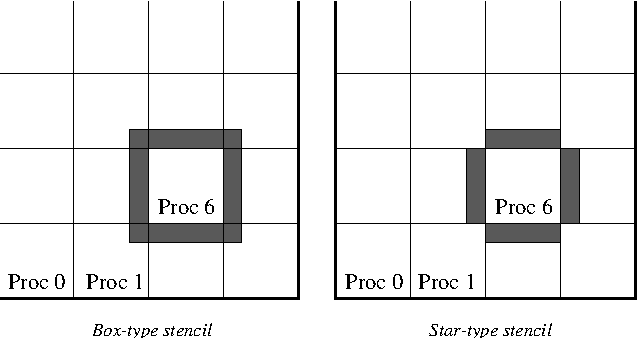
\includegraphics{ghost}}
%\centerline{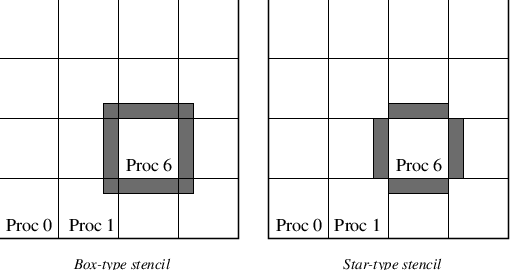
\psfig{file=ghost.eps,angle=0}}
\caption{Ghost Points for Two Stencil Types on the Seventh Process}
\label{fig_ghosts}
\end{figure}

\subsection{Creating Distributed Arrays}

The PETSc \lstinline{DMDA} object manages the parallel communication required
while working with data stored in regular arrays. The actual data
is stored in appropriately sized vector objects; the \lstinline{DMDA} object
only contains the parallel data layout information and communication
information, however it may be used to create vectors and matrices with the
proper layout.

One creates a distributed array communication data structure
in two dimensions with the command
\begin{lstlisting}
DMDACreate2d(MPI_Comm comm,DMBoundaryType xperiod,DMBoundaryType yperiod,DMDAStencilType st,PetscInt M, PetscInt N,PetscInt m,PetscInt n,PetscInt dof,PetscInt s,PetscInt *lx,PetscInt *ly,DM *da);
\end{lstlisting}
The  \sindex{array, distributed} arguments
\sindex{distributed array} \lstinline{M} and \lstinline{N} indicate the global
numbers of grid points in each direction, while \lstinline{m} and \lstinline{n}
denote the process partition in each direction; \lstinline{m*n} must equal
the number of processes in the MPI communicator, \lstinline{comm}.
Instead of specifying the process layout, one may use
\lstinline{PETSC_DECIDE} for \lstinline{m} and \lstinline{n}
so that PETSc will determine the partition using MPI. The type of
periodicity of the array is specified by \lstinline{xperiod} and \lstinline{yperiod}, which can be 
\lstinline{DM_BOUNDARY_NONE} \findex{DM_BOUNDARY_NONE} (no periodicity),
\lstinline{DM_BOUNDARY_PERIODIC} \findex{DM_BOUNDARY_PERIODIC} (periodic in that direction),
\lstinline{DM_BOUNDARY_TWIST} \findex{DM_BOUNDARY_TWIST} (periodic in that direction, but identified in reverse order),
\lstinline{DM_BOUNDARY_GHOSTED} \findex{DM_BOUNDARY_GHOSTED},
or \lstinline{DM_BOUNDARY_MIRROR}.\findex{DM_BOUNDARY_MIRROR}  The argument \lstinline{dof}
indicates the number of degrees of freedom at each array point,
and \lstinline{s} is the stencil width (i.e., the width of the ghost point region).
The optional arrays \lstinline{lx} and \lstinline{ly} may contain the number of nodes
along the x and y axis for each cell, i.e. the dimension of \lstinline{lx} is
\lstinline{m} and the dimension of \lstinline{ly} is \lstinline{n}; alternately, \lstinline{NULL} may be passed in.

Two types of distributed array communication data structures
can be created, as specified by \lstinline{st}.
Star-type stencils that radiate outward only in the coordinate
directions are indicated by \lstinline{DMDA_STENCIL_STAR},
while box-type stencils are specified by
\lstinline{DMDA_STENCIL_BOX}. For example, for the
two-dimensional case,
\lstinline{DMDA_STENCIL_STAR} with width 1 corresponds to the standard 5-point
stencil, while \lstinline{DMDA_STENCIL_BOX} with width 1 denotes the
standard 9-point stencil.  In both instances the ghost points are
identical, the only difference being that with star-type stencils
certain ghost points are ignored, decreasing substantially
the number of messages sent.  Note that the \lstinline{DMDA_STENCIL_STAR}
stencils can save interprocess communication in two and three
dimensions.

These DMDA stencils have nothing directly to do with any finite
difference stencils one might chose to use for a discretization; they
only ensure that the correct values are in place for application of a
user-defined finite difference stencil (or any other
discretization technique).

The commands for creating distributed array communication data structures
in one and three dimensions are analogous:
\begin{lstlisting}
DMDACreate1d(MPI_Comm comm,DMBoundaryType xperiod,PetscInt M,PetscInt w,PetscInt s,PetscInt *lc,DM *inra);
DMDACreate3d=(MPI_Comm comm,DMBoundaryType xperiod,DMBoundaryType yperiod,DMBoundaryType zperiod, DMDAStencilType stencil_type,PetscInt M,PetscInt N,PetscInt P,PetscInt m,PetscInt n,PetscInt p,PetscInt w,PetscInt s,PetscInt *lx,PetscInt *ly,PetscInt *lz,DM *inra);
\end{lstlisting}
The routines to create distributed arrays are collective, so that all
processes in the communicator \lstinline{comm} must call \lstinline{DACreateXXX()}.

%----------------------------------------------------------------------------------
\subsection{Local/Global Vectors and Scatters}

Each \lstinline{DMDA} object defines the layout of two vectors: a distributed
global vector and a local vector that includes room for the
appropriate ghost points.  The \lstinline{DMDA} object provides information
about the size and layout of these vectors, but does not internally
allocate any associated storage space for field values.  Instead, the
user can create vector objects that use the \lstinline{DMDA} layout
information with the routines
\begin{lstlisting}
DMCreateGlobalVector(DM da,Vec *g);
DMCreateLocalVector(DM da,Vec *l);
\end{lstlisting}
These vectors will generally serve as the building blocks for local
and global PDE solutions, etc.  If additional vectors with such
layout information are needed in a code, they can be obtained by
duplicating \lstinline{l} or \lstinline{g} via
\lstinline{VecDuplicate()} or \lstinline{VecDuplicateVecs()}.

We emphasize that a distributed array provides the information needed
to communicate the ghost value information between processes.  In most
cases, several different vectors can share the same communication
information (or, in other words, can share a given \lstinline{DMDA}).  The
design of the \lstinline{DMDA} object makes this easy, as each \lstinline{DMDA}
operation may operate on vectors of the appropriate size, as obtained
via \lstinline{DMCreateLocalVector()} and \lstinline{DMCreateGlobalVector()} or as
produced by \lstinline{VecDuplicate()}.  As such, the \lstinline{DMDA}
scatter/gather operations (e.g., \lstinline{DMGlobalToLocalBegin()}) require
vector input/output arguments, as discussed below.

PETSc currently provides no container for multiple arrays sharing the
same distributed array communication; note, however, that the \lstinline{dof}
parameter handles many cases of interest.

At certain stages of many applications, there is a need to work
on a local portion of the vector, including the ghost points.
This may be done by scattering a global vector into its
local parts by using the two-stage commands
\begin{lstlisting}
DMGlobalToLocalBegin(DM da,Vec g,InsertMode iora,Vec l);
DMGlobalToLocalEnd(DM da,Vec g,InsertMode iora,Vec l);
\end{lstlisting}
which allow the overlap of communication and computation.
Since the global and local vectors, given by \lstinline{g} and \lstinline{l}, respectively,
must be compatible with the distributed array, \lstinline{da}, they should be
generated by \lstinline{DMCreateGlobalVector()}
and \lstinline{DMCreateLocalVector()}
(or be duplicates of such a vector obtained via \lstinline{VecDuplicate()}).
The \lstinline{InsertMode} can be either \lstinline{ADD_VALUES} or \lstinline{INSERT_VALUES}.

One can scatter the local patches into the distributed vector
with the commands
\begin{lstlisting}
DMLocalToGlobalBegin(DM da,Vec l,InsertMode mode,Vec g);
DMLocalToGlobalEnd(DM da,Vec l,InsertMode mode,Vec g);
\end{lstlisting}
In general this is used with an \lstinline{InsertMode} of \lstinline{ADD_VALUES}, because if one wishes to insert values into the global vector they should
just access the global vector directly and put in the values.

A third type of distributed array scatter is from a local
vector (including ghost points that contain irrelevant values) to
a local vector with correct ghost point values.
This scatter may be done with the commands
\begin{lstlisting}
DMDALocalToLocalBegin(DM da,Vec l1,InsertMode iora,Vec l2);
DMDALocalToLocalEnd(DM da,Vec l1,InsertMode iora,Vec l2);
\end{lstlisting}
Since both local vectors, \lstinline{l1} and \lstinline{l2},
must be compatible with the distributed array, \lstinline{da}, they should be
generated by \lstinline{DMCreateLocalVector()}
(or be duplicates of such vectors obtained via \lstinline{VecDuplicate()}).
The \lstinline{InsertMode} can be either \lstinline{ADD_VALUES} or \lstinline{INSERT_VALUES}.

It is possible to directly access the vector scatter contexts (see below)
used in the local-to-global (\lstinline{ltog}), global-to-local
(\lstinline{gtol}), and local-to-local (\lstinline{ltol})
scatters with the command
\begin{lstlisting}
DMDAGetScatter(DM da,VecScatter *ltog,VecScatter *gtol,VecScatter *ltol);
\end{lstlisting}
Most users should not need to use these contexts.

\subsection{Local (Ghosted) Work Vectors}
In most applications the local ghosted vectors are only needed during user
``function evaluations''. PETSc provides an easy, light-weight (requiring
essentially no CPU time) way to obtain these work vectors and return them when
they are no longer needed. This is done with the routines
\begin{lstlisting}
DMGetLocalVector(DM da,Vec *l);
... use the local vector l ...
DMRestoreLocalVector(DM da,Vec *l);
\end{lstlisting}

\subsection{Accessing the Vector Entries for DMDA Vectors}
PETSc provides an easy way to set values into the DMDA Vectors and access them using
the natural grid indexing. This is done with the routines
\begin{lstlisting}
DMDAVecGetArray(DM da,Vec l,void *array);
... use the array indexing it with 1 or 2 or 3 dimensions ...
... depending on the dimension of the DMDA ...
DMDAVecRestoreArray(DM da,Vec l,void *array);
DMDAVecGetArrayRead(DM da,Vec l,void *array);
... use the array indexing it with 1 or 2 or 3 dimensions ...
... depending on the dimension of the DMDA ...
DMDAVecRestoreArrayRead(DM da,Vec l,void *array);
\end{lstlisting}
and
\begin{lstlisting}
DMDAVecGetArrayDOF(DM da,Vec l,void *array);
... use the array indexing it with 1 or 2 or 3 dimensions ...
... depending on the dimension of the DMDA ...
DMDAVecRestoreArrayDOF(DM da,Vec l,void *array);
DMDAVecGetArrayDOFRead(DM da,Vec l,void *array);
... use the array indexing it with 1 or 2 or 3 dimensions ...
... depending on the dimension of the DMDA ...
DMDAVecRestoreArrayDOFRead(DM da,Vec l,void *array);
\end{lstlisting}
where \lstinline{array} is a multidimensional C array with the same dimension as
\lstinline{da}. The vector \lstinline{l} can be either a global vector or a local vector.
The \lstinline{array} is accessed using the usual {\em global} indexing
on the entire grid, but the user may {\em only} refer to the local and ghost
entries of this array as all other entries are undefined. For example, for a
scalar problem in two dimensions one could use
\begin{lstlisting}
PetscScalar **f,**u;
...
DMDAVecGetArray(DM da,Vec local,&u);
DMDAVecGetArray(DM da,Vec global,&f);
...
  f[i][j] = u[i][j] - ...
...
DMDAVecRestoreArray(DM da,Vec local,&u);
DMDAVecRestoreArray(DM da,Vec global,&f);
\end{lstlisting}
The recommended approach for multi-component PDEs is to declare a \lstinline{struct} representing the fields defined at each node of the grid, e.g.
\begin{lstlisting}
typedef struct { 
  PetscScalar u,v,omega,temperature; 
} Node;
\end{lstlisting}
and write residual evaluation using
\begin{lstlisting}
Node **f,**u;
DMDAVecGetArray(DM da,Vec local,&u);
DMDAVecGetArray(DM da,Vec global,&f);
 ...
    f[i][j].omega = ...
 ...
DMDAVecRestoreArray(DM da,Vec local,&u);
DMDAVecRestoreArray(DM da,Vec global,&f);
\end{lstlisting}
See \href{http://www.mcs.anl.gov/petsc/petsc-current/src/snes/examples/tutorials/ex5.c.html}{\trl{$PETSC_DIR/src/snes/examples/tutorials/ex5.c}} for a 
complete example and see \href{http://www.mcs.anl.gov/petsc/petsc-current/src/snes/examples/tutorials/ex19.c.html}{\trl{$PETSC_DIR/src/snes/examples/tutorials/ex19.c}} for an
example for a multi-component PDE.

%---------------------------------------------------------------------------
\subsection{Grid Information}

The global indices of the lower left corner of the local portion of the array
as well as the local array size can be obtained with the commands
\begin{lstlisting}
DMDAGetCorners(DM da,PetscInt *x,PetscInt *y,PetscInt *z,PetscInt *m,PetscInt *n,PetscInt *p);
DMDAGetGhostCorners(DM da,PetscInt *x,PetscInt *y,PetscInt *z,PetscInt *m,PetscInt *n,PetscInt *p);
\end{lstlisting}
The first version excludes any ghost points, while the second version
includes them.
The routine \lstinline{DMDAGetGhostCorners()}
deals with the fact that subarrays along boundaries of the problem
domain have ghost points only on their interior edges, but not on
their boundary edges.

When either type of stencil is used, \lstinline{DMDA_STENCIL_STAR} or
\lstinline{DMDA_STENCIL_BOX}, the local vectors (with the ghost points)
represent rectangular arrays, including the extra corner elements in
the \lstinline{DMDA_STENCIL_STAR} case. This configuration provides simple
access to the elements by employing two- (or three-) dimensional indexing.
The only difference between the
two cases is that when \lstinline{DMDA_STENCIL_STAR} is used, the extra
corner components are {\em not} scattered between the processes and thus
contain undefined values that should {\em not} be used.

To assemble global stiffness matrices, one can use these global indices with \lstinline{MatSetValues()}
or \lstinline{MatSetValuesStencil()}.
Alternately, the global node number of each local node,
including the ghost nodes, can be obtained by calling
\begin{lstlisting}
DMGetLocalToGlobalMapping(DM da,ISLocalToGlobalMapping *map);
\end{lstlisting}
followed by
\begin{lstlisting}
VecSetLocalToGlobalMapping(Vec v,ISLocalToGlobalMapping map);
MatSetLocalToGlobalMapping(Mat A,ISLocalToGlobalMapping map);
\end{lstlisting}
Now entries may be added to the vector and matrix using the local numbering
and \break\lstinline{VecSetValuesLocal()} and \lstinline{MatSetValuesLocal()}.


Since the global ordering that PETSc uses to manage its parallel vectors
(and matrices) does not usually correspond to the ``natural'' ordering
of a two- or three-dimensional array, the \lstinline{DMDA} structure provides
an application ordering \lstinline{AO} (see Section \ref{sec_ao}) that maps
between the natural ordering on a rectangular grid and the ordering PETSc
uses to parallelize. This ordering context can be obtained with the command
\begin{lstlisting}
DMDAGetAO(DM da,AO *ao);
\end{lstlisting}
In Figure \ref{fig_daao} we indicate the orderings for a two-dimensional distributed
array, divided among four processes.

\begin{figure}[tb]
\centerline{ 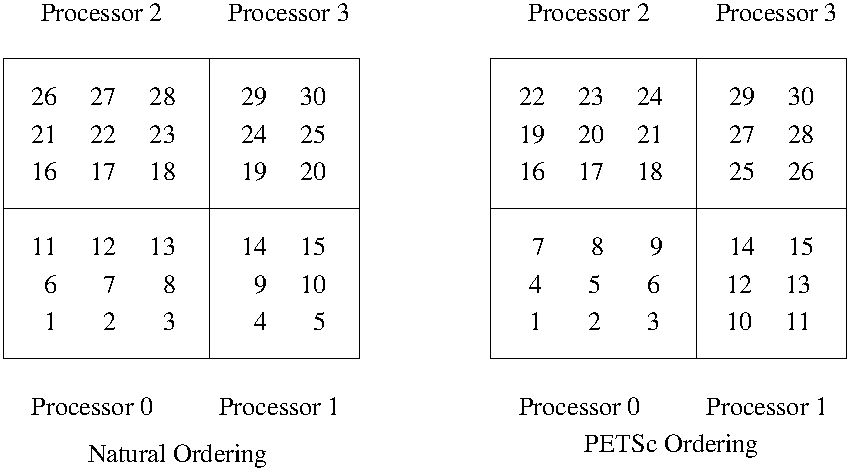
\includegraphics{danumbering}}
%\centerline{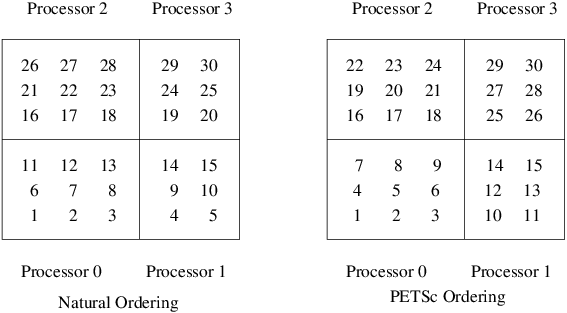
\psfig{file=danumbering.eps,angle=270,width=4.7in}}
\caption{Natural Ordering and PETSc Ordering for a 2D Distributed Array (Four Processes)}
\label{fig_daao}
\end{figure}

The example
\href{http://www.mcs.anl.gov/petsc/petsc-current/src/snes/examples/tutorials/ex5.c.html}{\trl{$PETSC_DIR/src/snes/examples/tutorials/ex5.c}}
illustrates the use of a distributed array in the solution of
a nonlinear problem.  The analogous Fortran program is
\href{http://www.mcs.anl.gov/petsc/petsc-current/src/snes/examples/tutorials/ex5.c.html}{\trl{$PETSC_DIR/src/snes/examples/tutorials/ex5.F}};
see Chapter \ref{chapter_snes} for a discussion of the nonlinear
solvers.

% --------------------------------------------------------------------------------------
\section{Vectors Related to Unstructured Grids}
\label{sec_unstruct}

% --------------------------------------------------------------------------------------
\subsection{Index Sets} \sindex{index sets}
\label{sec_indexset}

To facilitate general vector scatters and gathers used, for example, in updating
ghost points for problems defined on unstructured grids
\footnote{Also see Chapter \ref{ch_unstructured} which describes \lstinline{DMPlex}, an abstraction for working with unstructured grids.},
PETSc employs the concept of an {\em index set}, via the \lstinline{IS} class.  
An index set, which is a generalization of a
set of integer indices, is used to define scatters, gathers, and similar
operations on vectors and matrices.

The following command creates an index set based on a list
of integers:
\begin{lstlisting}
ISCreateGeneral(MPI_Comm comm,PetscInt n,PetscInt *indices,PetscCopyMode mode, IS *is);
\end{lstlisting}
When \lstinline{mode} is \lstinline{PETSC_COPY_VALUES}, this routine copies the \lstinline{n} indices passed
to it by the integer array \lstinline{indices}.
Thus, the user should be sure to free the integer array \lstinline{indices}
when it is no longer needed, perhaps directly after the call to
\lstinline{ISCreateGeneral()}. The communicator, \lstinline{comm}, should consist of all
processes that will be using the \lstinline{IS}.

Another standard index set is defined by a starting point (\lstinline{first}) and a
stride (\lstinline{step}), \sindex{stride} and can be created with the command
\begin{lstlisting}
ISCreateStride(MPI_Comm comm,PetscInt n,PetscInt first,PetscInt step,IS *is);
\end{lstlisting}

Index sets can be destroyed with the command
\begin{lstlisting}
ISDestroy(IS &is);
\end{lstlisting}

On rare occasions the user may need to access information directly from an index set.
Several commands assist in this process:
\begin{lstlisting}
ISGetSize(IS is,PetscInt *size);
ISStrideGetInfo(IS is,PetscInt *first,PetscInt *stride);
ISGetIndices(IS is,PetscInt **indices);
\end{lstlisting}
The function \lstinline{ISGetIndices()} returns a pointer to a list of the
indices in the index set.
For certain index sets, this may be a
temporary array of indices created specifically for a given routine.
Thus, once the user finishes using the array of indices,
the routine
\begin{lstlisting}
ISRestoreIndices(IS is, PetscInt **indices);
\end{lstlisting}
should be called to ensure that the system can free the space it
may have used to generate the list of indices.

A blocked version of the index sets can be created with the command
\begin{lstlisting}
ISCreateBlock(MPI_Comm comm,PetscInt bs,PetscInt n,PetscInt *indices,PetscCopyMode mode, IS *is);
\end{lstlisting}
This version is used for defining operations in which each element of the index
set refers to a block of \lstinline{bs} vector entries.  Related routines analogous
to those described above exist as well, including
\lstinline{ISBlockGetIndices()}, \lstinline{ISBlockGetSize()}, \lstinline{ISBlockGetLocalSize()}, \lstinline{ISGetBlockSize()}.
See the man pages for details.

% --------------------------------------------------------------------------------------
\subsection{Scatters and Gathers} \sindex{scatter} \sindex{gather}
\label{sec_scatter}

PETSc vectors have full support for general scatters and
gathers. One can select any subset of the components of a vector to
insert or add to any subset of the components of another vector.
We refer to these operations as {\em generalized scatters}, though they are
actually a combination of scatters and gathers. 

\findex{INSERT_VALUES} \findex{SCATTER_FORWARD}
To copy selected components from one vector
to another, one uses the following set of commands:
\begin{lstlisting}
VecScatterCreate(Vec x,IS ix,Vec y,IS iy,VecScatter *ctx);
VecScatterBegin(VecScatter ctx,Vec x,Vec y,INSERT_VALUES,SCATTER_FORWARD);
VecScatterEnd(VecScatter ctx,Vec x,Vec y,INSERT_VALUES,SCATTER_FORWARD);
VecScatterDestroy(VecScatter *ctx);
\end{lstlisting}
Here \lstinline{ix} denotes the index set of the first vector, while \lstinline{iy} 
indicates the index set of the destination vector.  The vectors
can be parallel or sequential. The only requirements are that the
number of entries in the index set of the first vector, \lstinline{ix},
equals the number in the destination index set, \lstinline{iy}, and that the
vectors be long enough to contain all the indices referred to in the
index sets.  The argument \lstinline{INSERT_VALUES} specifies that the
vector elements will be inserted into the specified locations of the
destination vector, overwriting any existing values.  To add the
components, rather than insert them, the user should select the option
\lstinline{ADD_VALUES} instead of \lstinline{INSERT_VALUES}.

To perform a conventional gather operation, the user simply makes
 the destination index set,
\lstinline{iy}, be a stride index set with a stride of one.  Similarly, a 
conventional scatter can be done with an initial (sending) index set
consisting of a stride.  The scatter routines are collective operations
(i.e. all processes that own
a parallel vector {\em must} call the scatter routines). When scattering from a
parallel vector to sequential vectors, each process has its own sequential
vector that receives values from locations as indicated in its own
index set. Similarly, in scattering
from sequential vectors to a parallel vector, each process has its
own sequential vector that makes contributions to the parallel vector.

{\em Caution}: When \lstinline{INSERT_VALUES} is used, if two different
processes contribute different values to the same component in a
parallel vector, either value may end up being inserted. When
\lstinline{ADD_VALUES} is used, the correct sum is added to the correct
location.

In some cases one may wish to ``undo'' a scatter, that is perform the
scatter backwards, switching the roles of the sender and receiver. This is
done by using
\begin{lstlisting}
VecScatterBegin(VecScatter ctx,Vec y,Vec x,INSERT_VALUES,SCATTER_REVERSE);
VecScatterEnd(VecScatter ctx,Vec y,Vec x,INSERT_VALUES,SCATTER_REVERSE);
\end{lstlisting}
Note that the roles of the first
two arguments to these routines must be swapped whenever the \lstinline{SCATTER_REVERSE}
option is used.

Once a \lstinline{VecScatter} object has been created it may be used with any vectors
that have the appropriate parallel data layout. That is, one can call
\lstinline{VecScatterBegin()} and \lstinline{VecScatterEnd()} with different vectors than
used in the call to \lstinline{VecScatterCreate()} so long as they have the same
parallel layout (number of elements on each process are the same). Usually,
these ``different'' vectors would have been obtained via calls to
\lstinline{VecDuplicate()} from the original vectors used in the call to
\lstinline{VecScatterCreate()}.

\sindex{vector values, getting}
There is a PETSc routine that is nearly the opposite of \lstinline{VecSetValues()}, that is, \lstinline{VecGetValues()}, but it can only get local values from the vector.
To get off-process values, the user should create a new vector where
the components are to be stored, and then perform the appropriate vector
scatter. For example, if one desires to obtain the values of the
100th and 200th entries of a parallel vector, \lstinline{p}, one could use
a code such as that within Figure~\ref{fig_vecscatter}.
In this example, the values of the 100th and 200th components are
placed in the array
values. In this example each process now has the 100th and
200th component, but obviously each process could gather any
elements it needed, or none by creating an index set with no entries.

\begin{figure}[tb]
\begin{lstlisting}
Vec         p, x;         /* initial vector, destination vector */
VecScatter  scatter;      /* scatter context */
IS          from, to;     /* index sets that define the scatter */
PetscScalar *values;
PetscInt    idx_from[] = {100,200}, idx_to[] = {0,1};

VecCreateSeq(PETSC_COMM_SELF,2,&x);
ISCreateGeneral(PETSC_COMM_SELF,2,idx_from,PETSC_COPY_VALUES,&from);
ISCreateGeneral(PETSC_COMM_SELF,2,idx_to,PETSC_COPY_VALUES,&to);
VecScatterCreate(p,from,x,to,&scatter);
VecScatterBegin(scatter,p,x,INSERT_VALUES,SCATTER_FORWARD);
VecScatterEnd(scatter,p,x,INSERT_VALUES,SCATTER_FORWARD);
VecGetArray(x,&values);
ISDestroy(&from);
ISDestroy(&to); 
VecScatterDestroy(&scatter);
\end{lstlisting}
\caption{Example Code for Vector Scatters}
\label{fig_vecscatter}
\end{figure}

The scatter comprises two stages, in order to allow overlap of
communication and computation. The introduction of the
\lstinline{VecScatter} context allows the communication patterns for the scatter
to be computed once and then reused repeatedly. Generally, even
setting up the communication for a scatter requires communication;
hence, it is best to reuse such information when possible.

% -------------------------------------------------------------------------------
\subsection{Scattering Ghost Values}

Generalized scatters provide a very general method for managing the communication of
required ghost values for unstructured grid computations. One scatters
the global vector into a local ``ghosted'' work vector, performs the computation
on the local work vectors, and then scatters back into the global solution
vector. In the simplest case this may be written as
\begin{lstlisting}
VecScatterBegin(VecScatter scatter,Vec globalin,Vec localin,InsertMode INSERT_VALUES, ScatterMode SCATTER_FORWARD);
VecScatterEnd(VecScatter scatter,Vec globalin,Vec localin,InsertMode INSERT_VALUES,ScatterMode SCATTER_FORWARD);
/* For example, do local calculations from localin to localout */
 ...
VecScatterBegin(VecScatter scatter,Vec localout,Vec globalout,InsertMode ADD_VALUES,ScatterMode SCATTER_REVERSE);
VecScatterEnd(VecScatter scatter,Vec localout,Vec globalout,InsertMode ADD_VALUES,ScatterMode SCATTER_REVERSE);
\end{lstlisting}

% -------------------------------------------------------------------------------
\subsection{Vectors with Locations for Ghost Values}
There are two minor drawbacks to the basic approach described above:
\begin{tightitemize}
\item the extra memory requirement for the local work vector, \lstinline{localin}, which
      duplicates the memory in \lstinline{globalin}, and
\item the extra time required to copy the local values from \lstinline{localin} to
      \lstinline{globalin}.
\end{tightitemize}

An alternative approach is to allocate global vectors with space preallocated for
the ghost values; this may be done with either
\begin{lstlisting}
VecCreateGhost(MPI_Comm comm,PetscInt n,PetscInt N,PetscInt nghost,PetscInt *ghosts,Vec *vv)
\end{lstlisting}
or
\begin{lstlisting}
VecCreateGhostWithArray(MPI_Comm comm,PetscInt n,PetscInt N,PetscInt nghost,PetscInt *ghosts,PetscScalar *array,Vec *vv)
\end{lstlisting}
Here  \lstinline{n} is the
number of local vector entries, \lstinline{N} is the number of \sindex{vectors, with ghost values}
global entries (or \lstinline{NULL}) and \lstinline{nghost} is the number of
ghost entries. The array \lstinline{ghosts} is of size \lstinline{nghost} and contains the
global vector location for each local ghost location. Using \lstinline{VecDuplicate()}
or \lstinline{VecDuplicateVecs()} on a ghosted vector will generate additional ghosted vectors.

In many ways, a ghosted vector behaves just like any other MPI vector created
by \lstinline{VecCreateMPI()}. The difference is that the ghosted vector has an additional
``local'' representation that allows one to access the ghost locations. This is done
through the call to
\begin{lstlisting}
VecGhostGetLocalForm(Vec g,Vec *l);
\end{lstlisting}
The vector \lstinline{l} is a
sequential representation of the parallel vector \lstinline{g}
that shares the same array space (and hence numerical values); but allows one to
access the ``ghost'' values past ``the end of the'' array. Note that one access the
entries in \lstinline{l} using the local numbering of elements and ghosts, while they
are accessed in \lstinline{g} using the global numbering.

A common usage of a ghosted vector is given by
\begin{lstlisting}
VecGhostUpdateBegin(Vec globalin,InsertMode INSERT_VALUES, ScatterMode SCATTER_FORWARD);
VecGhostUpdateEnd(Vec globalin,InsertMode INSERT_VALUES, ScatterMode SCATTER_FORWARD);
VecGhostGetLocalForm(Vec globalin,Vec *localin);
VecGhostGetLocalForm(Vec globalout,Vec *localout);
...  Do local calculations from localin to localout ...
VecGhostRestoreLocalForm(Vec globalin,Vec *localin);
VecGhostRestoreLocalForm(Vec globalout,Vec *localout);
VecGhostUpdateBegin(Vec globalout,InsertMode ADD_VALUES, ScatterMode SCATTER_REVERSE);
VecGhostUpdateEnd(Vec globalout,InsertMode ADD_VALUES, ScatterMode SCATTER_REVERSE);
\end{lstlisting}

The routines \lstinline{VecGhostUpdateBegin()} and \lstinline{VecGhostUpdateEnd()} are equivalent to the routines \lstinline{VecScatterBegin()} and \lstinline{VecScatterEnd()}
above except that since they are scattering into the ghost locations, they do not need
to copy the local vector values, which are already in place. In addition, the user does not
have to allocate the local work vector, since the ghosted vector already has allocated
slots to contain the ghost values.

The input arguments \lstinline{INSERT_VALUES} and \lstinline{SCATTER_FORWARD}
cause the ghost values to be correctly updated from the appropriate
process. The arguments \lstinline{ADD_VALUES} and \lstinline{SCATTER_REVERSE}
update the ``local'' portions of the vector from all the other
processes' ghost values.  This would be appropriate, for example,
when performing a finite element assembly of a load vector.

Section \ref{sec_partitioning} discusses the important topic of partitioning
an unstructured grid.

%-------------------------------------------------------------
%-------------------------------------------------------------
\cleardoublepage
\chapter{Matrices}
\label{chapter_matrices}
\sindex{matrices}

PETSc provides a variety of matrix implementations because no
single matrix format is appropriate for all problems.  Currently, we
support dense storage and compressed sparse row storage (both
sequential and parallel versions), as well as several specialized
formats.  Additional formats can be added.

This chapter describes the basics of using PETSc matrices in general
(regardless of the particular format chosen) and discusses tips for
efficient use of the several simple uniprocess and parallel matrix
types.  The use of PETSc matrices involves the following actions:
create a particular type of matrix, insert values into it, process the
matrix, use the matrix for various computations, and finally destroy
the matrix.  The application code does not need to know or care about
the particular storage formats of the matrices.

\section{Creating and Assembling Matrices}
\label{sec_matcreate}

The simplest routine for forming a PETSc matrix, \lstinline{A}, is
followed by
\begin{lstlisting}
MatCreate(MPI_Comm comm,Mat *A)
MatSetSizes(Mat A,PetscInt m,PetscInt n,PetscInt M,PetscInt N)
\end{lstlisting}
This routine generates a sequential matrix when running one
process and a parallel matrix for two or more processes; the
particular matrix format is set by the user via options database
commands.  The user specifies either the global matrix dimensions, given
by \lstinline{M} and \lstinline{N} or the local dimensions, given by \lstinline{m} and
\lstinline{n} while PETSc completely controls memory allocation.  This routine
facilitates switching among various matrix types, for example, to
determine the format that is most efficient for a certain
application.  By default, \lstinline{MatCreate()} employs the sparse AIJ
format, which is discussed in detail Section~\ref{sec_matsparse}.  See
the manual pages for further information about available matrix formats.

To insert or add entries to a matrix, one can call a variant of \lstinline{MatSetValues()}, either
\begin{lstlisting}
MatSetValues(Mat A,PetscInt m,const PetscInt idxm[],PetscInt n,const PetscInt idxn[],const PetscScalar values[],INSERT_VALUES);
\end{lstlisting}
or
\begin{lstlisting}
  MatSetValues(Mat A,PetscInt m,const PetscInt idxm[],PetscInt n,const PetscInt idxn[],const PetscScalar values[],ADD_VALUES);
\end{lstlisting}
This routine inserts or adds a logically dense subblock of dimension
\lstinline{m*n} into the
matrix. The integer indices \lstinline{idxm} and \lstinline{idxn}, respectively, indicate the
global row and column numbers to be inserted.  \lstinline{MatSetValues()} uses the
standard C convention, where the row and column matrix indices begin with
zero {\em regardless of the storage format employed}.   The array
\lstinline{values} is logically two-dimensional, containing the values that are
to be inserted. By default the values are given in row major order, which is the
opposite of the Fortran convention, meaning that the value to be put in row
\lstinline{idxm[i]} and column \lstinline{idxn[j]} is located in \lstinline{values[i*n+j]}. To
allow the insertion of values in column major order, one can call the command
\begin{lstlisting}
MatSetOption(Mat A,MAT_ROW_ORIENTED,PETSC_FALSE);
\end{lstlisting}
{\em Warning}: Several of the sparse implementations do {\em not} currently
support the column-oriented option.

This notation should not be a mystery to anyone. For example,
to insert one matrix into another when using MATLAB, one uses the command
\lstinline{A(im,in) = B;} where \lstinline{im} and \lstinline{in} contain the indices for the
rows and columns. This action is identical to the calls above to
\lstinline{MatSetValues()}.

When using the block compressed sparse row matrix format (\lstinline{MATSEQBAIJ} or
\lstinline{MATMPIBAIJ}), one can insert elements more efficiently using the block
variant, \lstinline{MatSetValuesBlocked()} or \break\lstinline{MatSetValuesBlockedLocal()}.

The function \lstinline{MatSetOption()} accepts several other inputs; see
the manual page for details.

After the matrix elements have been inserted or added into the matrix,
they must be processed (also called ``assembled'') before they can be used. The routines for matrix
processing are
\begin{lstlisting}
MatAssemblyBegin(Mat A,MAT_FINAL_ASSEMBLY);
MatAssemblyEnd(Mat A,MAT_FINAL_ASSEMBLY);
\end{lstlisting}
By placing other code between these two calls, the user can perform
computations while messages are in transit.
Calls to \lstinline{MatSetValues()} with the \lstinline{INSERT_VALUES} and
\lstinline{ADD_VALUES] options {\em cannot} be mixed without intervening calls to
the assembly routines.  For such intermediate assembly calls the
second routine argument  typically should be \lstinline{MAT_FLUSH_ASSEMBLY},
\findex{MAT_FLUSH_ASSEMBLY} which omits some of the work of the full
assembly process.  \lstinline{MAT_FINAL_ASSEMBLY} \findex{MAT_FINAL_ASSEMBLY} is
required only in the last matrix assembly before a matrix is used.

Even though one may insert values into PETSc matrices without regard
to which process eventually stores them, for efficiency
reasons we usually recommend generating most entries on the
process where they are destined to be stored.  To help the
application programmer with this task for matrices that are
distributed across the processes by ranges, the routine
\begin{lstlisting}
MatGetOwnershipRange(Mat A,PetscInt *first_row,PetscInt *last_row);
\end{lstlisting}
informs the user that all rows from \lstinline{first_row} to
\lstinline{last_row-1} (since the value returned in \lstinline{last_row} is one more
than the global index of the last local row) will be stored on the local process.

In the sparse matrix implementations, once the assembly routines have been called, the matrices are compressed and can be used for matrix-vector multiplication, etc.
Any space for preallocated nonzeros that was not filled by a call to \lstinline{MatSetValues()} or a related routine is compressed out by assembling with \lstinline{MAT_FINAL_ASSEMBLY}.
If you intend to use that extra space later, be sure to insert explicit zeros before assembling with \lstinline{MAT_FINAL_ASSEMBLY} so the space will not be compressed out.
Once the matrix has been assembled, inserting new values will be expensive since it will require copies and possible memory allocation.

If one wishes to repeatedly assemble matrices that retain the same
nonzero pattern (such as within a nonlinear or time-dependent
problem), the option
\begin{lstlisting}
MatSetOption(Mat A,MAT_NEW_NONZERO_LOCATIONS,PETSC_FALSE);
\end{lstlisting} \findex{MAT_NEW_NONZERO_LOCATIONS}
should be specified after the first matrix has been fully assembled.
This option ensures that certain data structures and communication
information will be reused (instead of regenerated) during successive
steps, thereby increasing efficiency.
See \href{http://www.mcs.anl.gov/petsc/petsc-current/src/ksp/ksp/examples/tutorials/ex5.c.html}{\trl{$PETSC_DIR/src/ksp/ksp/examples/tutorials/ex5.c}} for a simple example of
solving two linear systems that use the same matrix data structure.

\subsection{Sparse Matrices}
\label{sec_matsparse}

\sindex{AIJ matrix format} \sindex{CSR, compressed sparse row format}
The default matrix representation within PETSc is the general sparse
AIJ format (also called the Yale sparse matrix format or compressed
sparse row format, CSR).  This section discusses tips for {\em
efficiently} using this matrix format for large-scale
applications. Additional formats (such as block compressed row and
block diagonal storage, which are generally much more efficient for
problems with multiple degrees of freedom per node) are discussed
below.  Beginning users need not concern themselves initially with
such details and may wish to proceed directly to
Section~\ref{sec_matoptions}.  However, when an application code
progresses to the point of tuning for efficiency and/or generating
timing results, it is {\em crucial} to read this information.

\subsubsection{Sequential AIJ Sparse Matrices}

In the PETSc AIJ matrix formats, we store the nonzero elements
by rows, along with an array of corresponding column numbers and
an array of pointers to the beginning of each row.  Note that the
diagonal matrix entries are stored with the rest of the nonzeros (not
separately).

To create a sequential AIJ sparse matrix, \lstinline{A},
with \lstinline{m} rows and \lstinline{n} columns,
one uses the command
\begin{lstlisting}
MatCreateSeqAIJ(PETSC_COMM_SELF,PetscInt m,PetscInt n,PetscInt nz,PetscInt *nnz,Mat *A);
\end{lstlisting}
where \lstinline{nz} or \lstinline{nnz} can be used to preallocate matrix memory,
as discussed below. The user can set \lstinline{nz=0} and \lstinline{nnz=NULL} for PETSc to control all matrix memory allocation.

The sequential and parallel AIJ matrix storage formats by default
employ {\em i-nodes} (identical nodes) when possible.  We search for
consecutive rows with the same nonzero structure, thereby reusing
matrix information for increased efficiency.  Related options database
keys are \trl{-mat_no_inode} (do not use inodes) and \trl{
-mat_inode_limit <limit>} (set inode limit (max limit=5)).
Note that problems with a single degree of freedom per grid node
will automatically not use I-nodes.

By default, the internal data representation for the AIJ formats employs
zero-based indexing.  For compatibility with standard Fortran storage,
thus enabling use of external Fortran software packages such as
SPARSKIT, \sindex{SPARSKIT} the option \trl{-mat_aij_oneindex},
\findex{-mat_aij_oneindex} enables one-based indexing, where the stored
row and column indices begin at one, not zero.  All user calls to
PETSc routines, regardless of this option, use zero-based indexing.

\subsubsection{Preallocation of Memory for Sequential AIJ Sparse Matrices}

The dynamic process of allocating new memory and copying from the old
storage to the new is {\em intrinsically very expensive}.  Thus, to
obtain good performance when assembling an AIJ matrix, it is crucial
to preallocate the memory needed for the sparse matrix.  The user has
two choices for preallocating matrix memory via \lstinline{MatCreateSeqAIJ()}.

One can use the scalar \lstinline{nz} to specify the expected
number of nonzeros for each row.  This is generally fine if the number
of nonzeros per row is roughly the same throughout the matrix (or as a
quick and easy first step for preallocation).  If one underestimates
the actual number of nonzeros in a given row, then during the assembly
process PETSc will automatically allocate additional needed space.
However, this extra memory allocation can slow the computation,

If different rows have very different numbers of nonzeros, one
should attempt to indicate (nearly) the exact number of elements
intended for the various rows with the optional array, \lstinline{nnz} of
length \lstinline{m}, where \lstinline{m} is the number of rows, for example
\begin{lstlisting}
PetscInt nnz[m];
nnz[0] = <nonzeros in row 0>
nnz[1] = <nonzeros in row 1>
....
nnz[m-1] = <nonzeros in row m-1>
\end{lstlisting}
In this case, the assembly process will require no additional memory
allocations if the \lstinline{nnz} estimates are correct. If, however,
the \lstinline{nnz} estimates are incorrect, PETSc will automatically
obtain the additional needed space, at a slight loss of efficiency.

Using the array \lstinline{nnz} to preallocate memory is especially
important for efficient matrix assembly if the number of nonzeros
varies considerably among the rows.  One can generally set \lstinline{nnz}
either by knowing in advance the problem structure (e.g., the stencil
for finite difference problems on a structured grid) or by
precomputing the information by using a segment of code similar to
that for the regular matrix assembly.  The overhead of determining the
\lstinline{nnz} array will be quite small compared with the overhead of the
inherently expensive \lstinline{malloc}s and moves of data that are needed for
dynamic allocation during matrix assembly. Always guess high if an exact
value is not known (extra space is cheaper than too little).

Thus, when assembling a sparse matrix with very different
numbers of nonzeros in various rows, one could proceed
as follows for finite difference methods:
\begin{tightenumerate}
\item item Allocate integer array \lstinline{nnz}.
\item Loop over grid, counting the expected number of nonzeros for the row(s)
associated with the various grid points.
\item Create the sparse matrix via \lstinline{MatCreateSeqAIJ()} or alternative.
\item Loop over the grid, generating matrix entries and inserting
    in matrix via \lstinline{MatSetValues()}.
\end{tightenumerate}
For (vertex-based) finite element type calculations, an analogous procedure is as follows:
\begin{tightenumerate}
\item Allocate integer array \trl{nnz}.
\item Loop over vertices, computing the number of neighbor vertices, which determines the
 number of nonzeros for the corresponding matrix row(s).
\item Create the sparse matrix via \lstinline{MatCreateSeqAIJ()} or alternative.
\item Loop over elements, generating matrix entries and inserting
      in matrix via \lstinline{MatSetValues()}.
\end{tightenumerate}

The \trl{-info} \findex{-info} option causes the routines
\lstinline{MatAssemblyBegin()} and \lstinline{MatAssemblyEnd()} to print
information about the success of the preallocation.  Consider the
following example for the \lstinline{MATSEQAIJ} matrix format:
\begin{outputlisting}
MatAssemblyEnd_SeqAIJ:Matrix size 10 X 10; storage space:20 unneeded, 100 used
MatAssemblyEnd_SeqAIJ:Number of mallocs during MatSetValues is 0
\end{outputlisting}
The first line indicates that the user preallocated 120 spaces but only
100 were used. The second line indicates that the user preallocated
enough space so that PETSc did not have to internally allocate additional
space (an expensive operation).  In the next example the user did not
preallocate sufficient space, as indicated by the fact that the number
of mallocs is very large (bad for efficiency):
\begin{outputlisting}
MatAssemblyEnd_SeqAIJ:Matrix size 10 X 10; storage space:47 unneeded, 1000 used
MatAssemblyEnd_SeqAIJ:Number of mallocs during MatSetValues is 40000
\end{outputlisting}

Although at first glance such procedures for determining the matrix
structure in advance may seem unusual, they are actually very
efficient because they alleviate the need for dynamic
construction of the matrix data structure, which can be very
expensive.

\subsubsection{Parallel AIJ Sparse Matrices}

Parallel sparse matrices with the AIJ
format can be created with the command
\begin{lstlisting}
MatCreateAIJ=(MPI_Comm comm,PetscInt m,PetscInt n,PetscInt M,PetscInt N,PetscInt d_nz,PetscInt *d_nnz, PetscInt o_nz,PetscInt *o_nnz,Mat *A);
\end{lstlisting}
\lstinline{A} is the newly created matrix, while the arguments \lstinline{m},
\lstinline{M}, and \lstinline{N}, indicate the number of local rows and
the number of global rows and columns, respectively. In the PETSc partitioning scheme,
all the matrix columns are local and \lstinline{n} is the number of columns
corresponding to local part of a parallel vector.
Either the local or
global parameters can be replaced with \lstinline{PETSC_DECIDE}, so that
PETSc will determine \findex{PETSC_DECIDE} them.
The matrix is stored with a fixed number of rows on
each process, given by \lstinline{m}, or determined by PETSc if \lstinline{m} is
\lstinline{PETSC_DECIDE}.

If \lstinline{PETSC_DECIDE} is not used for the arguments
\lstinline{m} and \lstinline{n}, then the user must ensure that they are chosen to be
compatible with the vectors. To do this, one first considers the matrix-vector product
$y = A x$. The \lstinline{m} that is used in the matrix creation routine \lstinline{MatCreateAIJ()}
must match the local size used in the vector creation routine \lstinline{VecCreateMPI()} for \lstinline{y}.
Likewise, the \lstinline{n} used must match that used as the local size in
\lstinline{VecCreateMPI()} for \lstinline{x}.

The user must set \lstinline{d_nz=0}, \lstinline{o_nz=0}, \lstinline{d_nnz=}NULL, and
\lstinline{o_nnz=NULL} for PETSc to control dynamic allocation of matrix
memory space.  Analogous to \lstinline{nz} and \lstinline{nnz} for the routine
\break\lstinline{MatCreateSeqAIJ()}, these arguments optionally specify
nonzero information for the diagonal (\lstinline{d_nz} and \lstinline{d_nnz}) and
off-diagonal (\lstinline{o_nz} and \lstinline{o_nnz}) parts of the matrix.
For a square global matrix, we define each process's diagonal portion
to be its local rows and the corresponding columns (a square submatrix);
each process's off-diagonal portion encompasses the remainder of the
local matrix (a rectangular submatrix).
The rank in the MPI communicator determines the absolute ordering of the
blocks.  That is, the process with rank 0 in the communicator given to  \lstinline{MatCreateAIJ()} contains the top rows of the matrix; the i$^{th}$ process
in that communicator contains the i$^{th}$ block of the matrix.

\subsubsection{Preallocation of Memory for Parallel AIJ Sparse Matrices}

As discussed above, preallocation of memory is critical for achieving good
performance during matrix assembly, as this reduces the number of
allocations and copies required.  We present an example for
three processes to indicate how this may be done for the \lstinline{MATMPIAIJ}
matrix format.  Consider the 8 by
8 matrix, which is partitioned by default with three rows on the first
process, three on the second and two on the third.  {\small
\[
\left( \begin{array}{cccccccccc}
1  & 2  & 0  & | & 0  & 3  & 0  & |  & 0  & 4  \\
0  & 5  & 6  & | & 7  & 0  & 0  & |  & 8  & 0 \\
9  & 0  & 10 & | & 11 & 0  & 0  & |  & 12 & 0  \\
\hline \\
13 & 0  & 14 & | & 15 & 16 & 17 & |  & 0  & 0  \\
0  & 18 & 0  & | & 19 & 20 & 21 & |  & 0  & 0 \\
0  & 0  & 0  & | & 22 & 23 & 0  & |  & 24 & 0 \\
\hline \\
25 & 26 & 27 & | & 0  & 0  & 28 & |  & 29 & 0 \\
30 & 0  & 0  & | & 31 & 32 & 33 & |  & 0  &34
\end{array} \right)
\]
}

The ``diagonal'' submatrix, \lstinline{d}, on the first process is given by
{\small
\[
\left( \begin{array}{ccc}
1  & 2  & 0  \\
0  & 5  & 6  \\
9  & 0  & 10
\end{array} \right),
\]
}
while the ``off-diagonal'' submatrix, \lstinline{o}, matrix is given by
{\small
\[
\left( \begin{array}{ccccc}
 0  & 3  & 0   & 0  & 4  \\
 7  & 0  & 0   & 8  & 0  \\
 11 & 0  & 0   & 12 & 0  \\
\end{array} \right).
\]
}
For the first process one could set \lstinline{d_nz} to 2 (since each
row has 2 nonzeros) or, alternatively, set \lstinline{d_nnz} to $\{2,2,2\}.$
The \lstinline{o_nz} could be set to 2 since each row of the \lstinline{o} matrix
has 2 nonzeros, or \lstinline{o_nnz} could be set to $\{2,2,2\}$.

For the second process the \lstinline{d} submatrix is given by
{\small
\[
\left( \begin{array}{cccccccccc}
 15 & 16 & 17 \\
 19 & 20 & 21 \\
 22 & 23 & 0
\end{array} \right) .
\]
}
Thus, one could set \lstinline{d_nz} to 3, since the maximum number of
nonzeros in each row is 3, or alternatively one could set \lstinline{d_nnz} to
$\{3,3,2\}$, thereby indicating that the first two rows will have 3
nonzeros while the third has 2. The corresponding \lstinline{o} submatrix for the
second process is
{\small
\[
\left( \begin{array}{cccccccccc}
13 & 0  & 14 &  0  & 0  \\
0  & 18 & 0  &  0  & 0 \\
0  & 0  & 0  &  24 & 0 \\
\end{array} \right)
\]
}
so that one could set \lstinline{o_nz} to 2 or \lstinline{o_nnz} to \{2,1,1\}.

Note that the user never directly works with the \lstinline{d} and \lstinline{o}
submatrices, except when preallocating storage space as indicated above.
Also, the user need not preallocate exactly the correct amount of
space; as long as a sufficiently close estimate is given, the high
efficiency for matrix assembly will remain.

As described above, the option \trl{-info} \findex{-info}
will print information about the success of preallocation during
matrix assembly.  For the \lstinline{MATMPIAIJ} and \lstinline{MATMPIBAIJ} formats, PETSc will also list
the number of elements owned by on each process that were generated
on a different process.  For example, the statements
\begin{outputlisting}
MatAssemblyBegin_MPIAIJ:Stash has 10 entries, uses 0 mallocs 
MatAssemblyBegin_MPIAIJ:Stash has 3 entries, uses 0 mallocs 
MatAssemblyBegin_MPIAIJ:Stash has 5 entries, uses 0 mallocs
\end{outputlisting}
indicate that very few values have been generated on different processes.
On the other hand, the statements
\begin{outputlisting}
MatAssemblyBegin_MPIAIJ:Stash has 100000 entries, uses 100 mallocs 
MatAssemblyBegin_MPIAIJ:Stash has 77777 entries, uses 70 mallocs
\end{outputlisting}
indicate that many values have been generated on the ``wrong'' processes.
This situation can be very inefficient, since the transfer of values
to the ``correct'' process is generally expensive.  By using the command
\lstinline{MatGetOwnershipRange()} in application codes, the user should be able
to generate most entries on the owning process.

{\em Note}: It is fine to generate some entries on the ``wrong'' process. Often
this can lead to cleaner, simpler, less buggy codes.  One should never
make code overly complicated in order to generate all values locally. Rather,
one should organize the code in such a way that {\em most} values are generated locally.

\subsection{Dense Matrices}
\label{sec_matdense}

PETSc provides both sequential and parallel dense matrix formats,
where each process stores its entries in a column-major array in the
usual Fortran style.  To create a sequential, dense PETSc matrix,
\lstinline{A} of dimensions \lstinline{m} by \lstinline{n}, the user should
call
\begin{lstlisting}
MatCreateSeqDense(PETSC_COMM_SELF,PetscInt m,PetscInt n,PetscScalar *data,Mat *A);
\end{lstlisting}
The variable \lstinline{data} enables the user to optionally provide the
location of the data for matrix storage (intended for Fortran users who
wish to allocate their own storage space).  Most users should merely
set \lstinline{data} to \lstinline{NULL} for PETSc to control matrix memory allocation.
To create a parallel, dense matrix, \lstinline{A}, the user should call
\begin{lstlisting}
MatCreateDense(MPI_Comm comm,PetscInt m,PetscInt n,PetscInt M,PetscInt N,PetscScalar *data,Mat *A)
\end{lstlisting}
The arguments \lstinline{m}, \lstinline{n},
\lstinline{M}, and \lstinline{N}, indicate the number of local rows and columns and
the number of global rows and columns, respectively. Either the local or
global parameters can be replaced with \lstinline{PETSC_DECIDE}, so that
PETSc will determine them.
The matrix is stored with a fixed number of rows on
each process, given by \lstinline{m}, or determined by PETSc if \lstinline{m} is
\lstinline{PETSC_DECIDE}.

PETSc does not provide parallel dense direct solvers, instead interfacing to external packages that provide these solvers. Our focus is on sparse iterative solvers.

\subsection{Block Matrices}
\label{sec_matnest}
Block matrices arise when coupling variables with different meaning, especially when solving problems with constraints (e.g. incompressible flow) and ``multi-physics'' problems.
Usually the number of blocks is small and each block is partitioned in parallel.
We illustrate for a $3\times 3$ system with components labeled $a,b,c$.
With some numbering of unknowns, the matrix could be written as
\[
\left( \begin{array}{ccc}
    A_{aa} & A_{ab} & A_{ac} \\
    A_{ba} & A_{bb} & A_{bc} \\
    A_{ca} & A_{cb} & A_{cc}
  \end{array} \right) .
\]
There are two fundamentally different ways that this matrix could be stored, as a single assembled sparse matrix where entries from all blocks are merged together (``monolithic''), or as separate assembled matrices for each block (``nested'').
These formats have different performance characteristics depending on the operation being performed.
In particular, many preconditioners require a monolithic format, but some that are very effective for solving block systems (see Section~\ref{sec_block_matrices}) are more efficient when a nested format is used.
In order to stay flexible, we would like to be able to use the same code to assemble block matrices in both monolithic and nested formats.
Additionally, for software maintainability and testing, especially in a multi-physics context where different groups might be responsible for assembling each of the blocks, it is desirable to be able to use exactly the same code to assemble a single block independently as to assemble it as part of a larger system.
To do this, we introduce the four spaces shown in Figure~\ref{fig_localspaces}.
\begin{itemize}
\item The monolithic global space is the space in which the Krylov and Newton solvers operate, with collective semantics across the entire block system.
\item The split global space splits the blocks apart, but each split still has collective semantics.
\item The split local space adds ghost points and separates the blocks.
  Operations in this space can be performed with no parallel communication.
  This is often the most natural, and certainly the most powerful, space for matrix assembly code.
\item The monolithic local space can be thought of as adding ghost points to the monolithic global space, but it is often more natural to use it simply as a concatenation of split local spaces on each process.
  It is not common to explicitly manipulate vectors or matrices in this space (at least not during assembly), but it is a useful for declaring which part of a matrix is being assembled.
\end{itemize}

\begin{figure}
\centerline{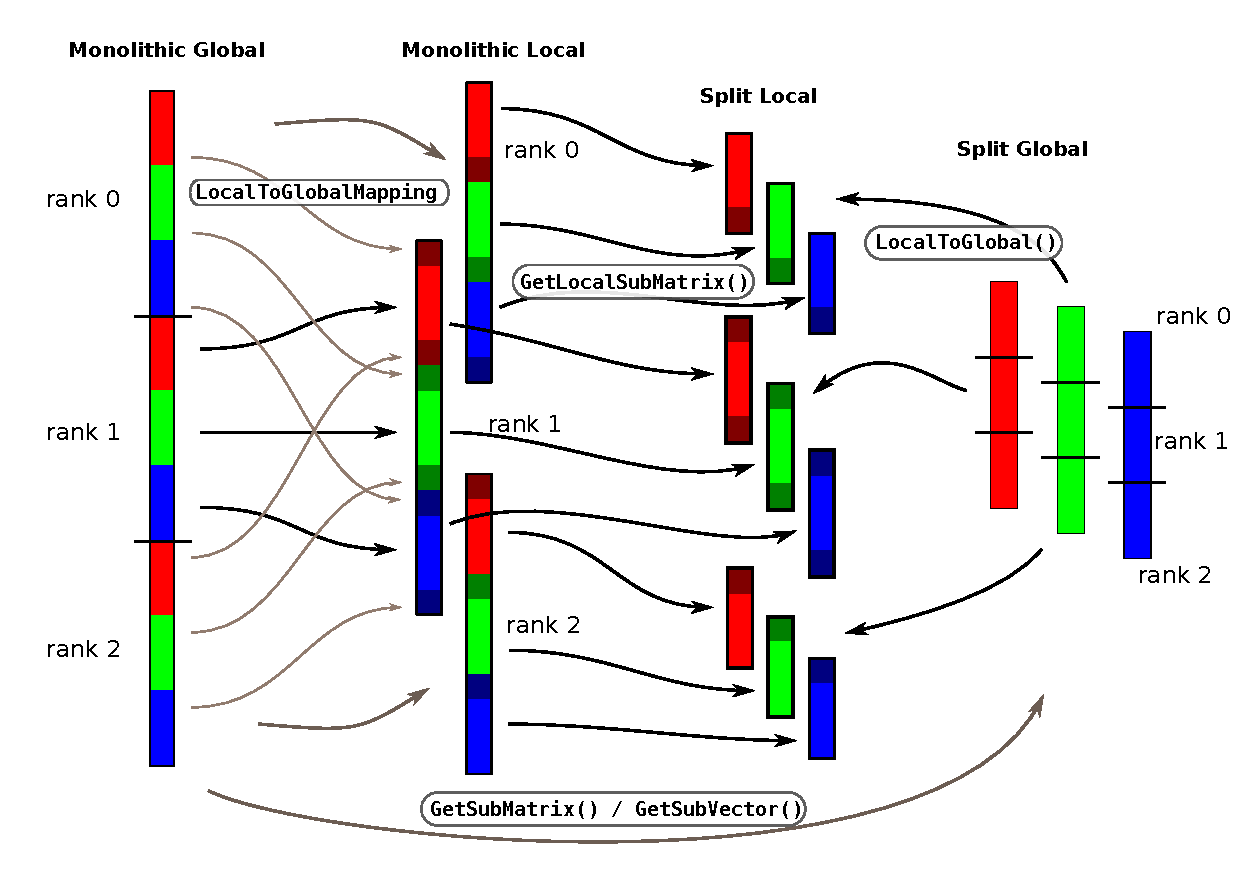
\includegraphics[width=\textwidth]{localspaces}}
\caption{The relationship between spaces used for coupled assembly.}
\label{fig_localspaces}
\end{figure}

The key to format-independent assembly is the function
\begin{lstlisting}
MatGetLocalSubMatrix(Mat A,IS isrow,IS iscol,Mat *submat);
\end{lstlisting}
which provides a ``view'' \lstinline{submat} into a matrix \lstinline{A} that operates in the monolithic global space.
The \lstinline{submat} transforms from the split local space defined by \lstinline{iscol} to the split local space defined by \lstinline{isrow}.
The index sets specify the parts of the monolithic local space that \lstinline{submat} should operate in.
If a nested matrix format is used, then \lstinline{MatGetLocalSubMatrix()} finds the nested block and returns it without making any copies.
In this case, \lstinline{submat} is fully functional and has a parallel communicator.
If a monolithic matrix format is used, then \lstinline{MatGetLocalSubMatrix()} returns a proxy matrix on \lstinline{PETSC_COMM_SELF} that does not provide values or implement \lstinline{MatMult()}, but does implement \lstinline{MatSetValuesLocal()} and, if \lstinline{isrow,iscol} have a constant block size, \lstinline{MatSetValuesBlockedLocal()}.
Note that although \lstinline{submat} may not be a fully functional matrix and the caller does not even know a priori which communicator it will reside on, it always implements the local assembly functions (which are not collective).
The index sets \lstinline{isrow,iscol} can be obtained using \break\lstinline{DMCompositeGetLocalISs()} if \lstinline{DMComposite} is being used.
DMComposite can also be used to create matrices, in which case the MATNEST format can be specified using \trl{-prefix_dm_mat_type nest} and MATAIJ can be specified using \trl{-prefix_dm_mat_type aij}.
See \href{http://www.mcs.anl.gov/petsc/petsc-current/src/snes/examples/tutorials/ex28.c.html}{\trl{$PETSC_DIR/src/snes/examples/tutorials/ex28.c}} for a simple example using this interface.

\section{Basic Matrix Operations}
\label{sec_matoptions}

Table \ref{fig_matrixops} summarizes basic PETSc matrix operations.
We briefly discuss a few of these routines in more detail below.

The parallel matrix can multiply a vector with \lstinline{n}
local entries, returning a vector with \lstinline{m} local entries. That is,
to form the product
\begin{lstlisting}
MatMult(Mat A,Vec x,Vec y);
\end{lstlisting}
the vectors \lstinline{x} and \lstinline{y} should be generated with
\begin{lstlisting}
VecCreateMPI(MPI_Comm comm,n,N,&x);
VecCreateMPI(MPI_Comm comm,m,M,&y);
\end{lstlisting}
By default, if the user lets PETSc decide the number of components to
be stored locally (by passing in \lstinline{PETSC_DECIDE} as the second
argument to \lstinline{VecCreateMPI()} or using \lstinline{VecCreate()}), vectors
and matrices of the same dimension are automatically compatible for
parallel matrix-vector operations.

Along with the matrix-vector multiplication routine, there is
a version for the transpose of the matrix,
\begin{lstlisting}
MatMultTranspose(Mat A,Vec x,Vec y);
\end{lstlisting}
There are also versions that add the result
to another vector:
\begin{lstlisting}
MatMultAdd(Mat A,Vec x,Vec y,Vec w);
MatMultTransposeAdd(Mat A,Vec x,Vec y,Vec w);
\end{lstlisting}
These routines, respectively, produce $ w = A*x + y $ and $ w = A^{T}*x + y$ .
In C it is legal for the vectors \lstinline{y} and \lstinline{w} to be identical.
In Fortran, this situation is forbidden by the language standard,
but we allow it anyway.

One can print a matrix (sequential or parallel) to the screen with the
command
\begin{lstlisting}
MatView(Mat mat,PETSC_VIEWER_STDOUT_WORLD);
\end{lstlisting}
Other viewers can be used as well. For instance, one can draw the
nonzero structure of the matrix into the default X-window with the
command
\begin{lstlisting}
MatView(Mat mat,PETSC_VIEWER_DRAW_WORLD);
\end{lstlisting}
Also one can use
\begin{lstlisting}
MatView(Mat mat,PetscViewer viewer);
\end{lstlisting}
where \lstinline{viewer} was obtained with \lstinline{PetscViewerDrawOpen()}.
Additional viewers and options are given in the \lstinline{MatView()} man
page and Section~\ref{sec_viewers}.

\begin{table}[tb]
\begin{center}
\begin{tabular}{ll}
{\bf Function Name} & {\bf Operation} \\
\hline
\lstinline|MatAXPY(Mat Y, PetscScalar a, Mat X, MatStructure s);| & $ Y = Y + a*X $ \\
\lstinline|MatMult(Mat A,Vec x, Vec y);| & $ y = A*x $ \\
\lstinline|MatMultAdd(Mat A,Vec x, Vec y,Vec z);| & $ z = y + A*x $ \\
\lstinline|MatMultTranspose(Mat A,Vec x, Vec y);| & $ y = A^{T}*x $ \\
\lstinline|MatMultTransposeAdd(Mat A, Vec x, Vec y, Vec z);| & $ z = y + A^{T}*x $ \\
\lstinline|MatNorm(Mat A,NormType type, PetscReal *r);| & $ r = ||A||_{type}$ \\
\lstinline|MatDiagonalScale(Mat A,Vec l,Vec r);| & $ A = \hbox{diag}(l)*A*\hbox{diag}(r) $ \\
\lstinline|MatScale(Mat A,PetscScalar a);| & $ A = a*A $ \\
\lstinline|MatConvert(Mat A, MatType type, Mat *B);| & $ B = A $ \\
\lstinline|MatCopy(Mat A, Mat B, MatStructure s);| &  $ B = A $ \\
\lstinline|MatGetDiagonal(Mat A, Vec x);| & $ x = \hbox{diag}(A)$ \\
\lstinline|MatTranspose(Mat A, MatReuse, Mat* B);| & $ B = A^{T} $ \\
\lstinline|MatZeroEntries(Mat A);| & $ A = 0 $ \\
\lstinline|MatShift(Mat Y, PetscScalar a);| & $ Y =  Y + a*I $ \\
\hline
\end{tabular}
\end{center}
\caption{\hbox{PETSc Matrix Operations}}
\label{fig_matrixops}
\end{table}
The \lstinline{NormType} argument to \lstinline{MatNorm()} is one of
\lstinline{NORM_1}, \lstinline{NORM_INFINITY}, and \lstinline{NORM_FROBENIUS}.

\sindex{1-norm} \sindex{infinity norm} \sindex {Frobenius norm}
\section{Matrix-Free Matrices} \sindex{matrix-free methods}
\label{sec_matrixfree}
Some people like to use matrix-free methods, which do not require
explicit storage of the matrix, for the numerical solution of partial
differential equations.  To support matrix-free methods in PETSc, one
can use the following command to create a \lstinline{Mat} structure without
ever actually generating the matrix:
\begin{lstlisting}
MatCreateShell(MPI_Comm comm,PetscInt m,PetscInt n,PetscInt M,PetscInt N,void *ctx,Mat *mat);
\end{lstlisting}
Here \lstinline{M} and \lstinline{N} are the global matrix dimensions (rows and
columns), \lstinline{m} and \lstinline{n} are the local matrix dimensions, and
\trl{ctx} is a pointer to data needed by any user-defined shell matrix
operations; the manual page has additional details about these
parameters.  Most matrix-free algorithms require only the application
of the linear operator to a vector. To provide this action, the user
must write a routine with the calling sequence
\begin{lstlisting}
UserMult(Mat mat,Vec x,Vec y);
\end{lstlisting}
and then associate it with the matrix, \lstinline{mat}, by using the
command
\begin{lstlisting}
MatShellSetOperation(Mat mat,MatOperation MATOP_MULT, (void(*)(void)) PetscErrorCode (*UserMult)(Mat,Vec,Vec));
\end{lstlisting}
Here \lstinline{MATOP_MULT} is the name of the operation for matrix-vector
multiplication. Within each user-defined routine (such as
\lstinline{UserMult()}), the user should call
\lstinline{MatShellGetContext()} to obtain the user-defined context, \lstinline{ctx},
that was set by \lstinline{MatCreateShell()}.
This shell matrix can be used with the iterative linear
equation solvers discussed in the following chapters.

The routine \lstinline{MatShellSetOperation()} can be used to set any other
matrix operations as well.  The file
\href{http://www.mcs.anl.gov/petsc/petsc-current/include/petscmat.h.html}{\trl{$PETSC_DIR/include/petscmat.h}} provides a complete list of matrix
operations, which have the form \lstinline{MATOP_<OPERATION>}, where \lstinline{<OPERATION>} is the name (in all capital letters) of the user
interface routine (for example, \lstinline{MatMult()} $ \to $ \lstinline{MATOP_MULT}).  All
user-provided functions have the same calling sequence as the
usual matrix interface routines, since the user-defined functions are
intended to be accessed through the same interface, e.g.,
\lstinline{MatMult(Mat,Vec,Vec)} $ \to$ \lstinline{UserMult(Mat,Vec,Vec)}.
The final argument for \lstinline{MatShellSetOperation()} needs to be cast
to a \lstinline{void *}, since the final argument could (depending on the
MatOperation) be a variety of different functions.

Note that \lstinline{MatShellSetOperation()} can also be used as a
``backdoor'' means of introducing user-defined changes in matrix
operations for other storage formats (for example, to override the
default LU factorization routine supplied within PETSc for the
\lstinline{MATSEQAIJ} format).  However, we urge anyone who introduces such
changes to use caution, since it would be very easy to
accidentally create a bug in the new routine that could affect
other routines as well.

See also Section~\ref{sec_nlmatrixfree} for details on one set of
helpful utilities for using the matrix-free approach for nonlinear
solvers.

\section{Other Matrix Operations}
\label{sec_othermat}

In many iterative calculations (for instance, in a nonlinear equations
solver), it is important for efficiency purposes to reuse the nonzero
structure of a matrix, rather than determining it anew every time
the matrix is generated.  To retain a given matrix but reinitialize
its contents, one can employ
\begin{lstlisting}
MatZeroEntries(Mat A);
\end{lstlisting}
This routine will zero the matrix entries in the
data structure but keep all the data that indicates where the nonzeros
are located.  In this way a new matrix assembly will be much less
expensive, since no memory allocations or copies will be needed.
Of course, one can also explicitly set selected matrix elements to zero
by calling \lstinline{MatSetValues()}.

By default, if new entries are made in locations where no nonzeros
previously existed, space will be allocated for the new entries.
To prevent the allocation of additional memory and simply discard those
new entries, one can use the option
\begin{lstlisting}
MatSetOption(Mat A,MAT_NEW_NONZERO_LOCATIONS,PETSC_FALSE);
\end{lstlisting}
Once the matrix has been assembled, one can factor it numerically
without repeating the ordering or the symbolic factorization.
This option can save some computational time, although it
does require that the factorization is not done in-place.

In the numerical solution of elliptic partial differential equations,
it can be cumbersome to deal with Dirichlet boundary
\sindex{boundary conditions} conditions. In
particular, one would like to assemble the matrix without regard to
boundary conditions and then at the end apply the Dirichlet boundary
conditions.
In numerical analysis classes this process is usually presented as moving the
known boundary conditions to the right-hand side and then solving a smaller
linear system for the interior unknowns. Unfortunately, implementing this
requires extracting a large submatrix from the original matrix and
creating its corresponding data structures. This process can be expensive
in terms of both time and memory.

One simple way to deal with this difficulty is to replace those rows in the
matrix associated with known boundary conditions, by rows of the
identity matrix (or some scaling of it). This action can be done with
the command
\begin{lstlisting}
MatZeroRows(Mat A,PetscInt numRows,PetscInt rows[],PetscScalar diag_value,Vec x,Vec b),
\end{lstlisting}
or equivalently,
\begin{lstlisting}
MatZeroRowsIS(Mat A,IS rows,PetscScalar diag_value,Vec x,Vec b);
\end{lstlisting}
For sparse matrices this removes the data structures for certain rows
of the matrix. If the pointer \lstinline{diag_value} is \lstinline{NULL}, it
even removes the diagonal entry. If the pointer is not null, it uses that
given value at the pointer location
in the diagonal entry of the eliminated rows.

One nice feature of this approach is that when solving a nonlinear problem
such that at each iteration the Dirichlet boundary conditions are in the
same positions and the matrix retains the same nonzero structure, the user
can call \lstinline{MatZeroRows()} in the first iteration. Then, before generating
the matrix in the second iteration the user should call
\begin{lstlisting}
MatSetOption(Mat A,MAT_NEW_NONZERO_LOCATIONS,PETSC_FALSE);
\end{lstlisting}
From that point,
no new values will be inserted into those (boundary) rows of
the matrix. \findex{MAT_NEW_NONZERO_LOCATIONS}

The functions \lstinline{MatZeroRowsLocal()} and \lstinline{MatZeroRowsLocalIS()} can also be used if for each process one provides the Dirichlet locations in the local numbering of the matrix.
A drawback of \lstinline{MatZeroRows()} is that it destroys the symmetry of a matrix. Thus one can use
\begin{lstlisting}
MatZeroRowsColumns(Mat A,PetscInt numRows,PetscInt rows[],PetscScalar diag_value,Vec x,Vec b),
\end{lstlisting}
or equivalently,
\begin{lstlisting}
MatZeroRowsColumnsIS(Mat A,IS rows,PetscScalar diag_value,Vec x,Vec b);
\end{lstlisting}
Note that with all of these for a given assembled matrix it can be
only called once to update the x and b vector. It cannot be used if
one wishes to solve multiple right hand side problems for the same
matrix since the matrix entries needed for updating the b vector are
removed in its first use.

Once the zeroed rows are removed the new matrix has possibly many rows
with only a diagonal entry affecting the parallel load balancing. The
\lstinline{PCREDISTRIBUTE} preconditioner removes all the zeroed rows (and
associated columns and adjusts the right hand side based on the
removed columns) and then rebalances the resulting rows of smaller
matrix across the processes. Thus one can use \lstinline{MatZeroRows()} to set the Dirichlet points and then solve with the preconditioner \lstinline{PCREDISTRIBUTE}. Note if the original matrix was symmetric the
smaller solved matrix will also be symmetric.

Another matrix routine of interest is
\begin{lstlisting}
MatConvert(Mat mat,MatType newtype,Mat *M)
\end{lstlisting}
which converts the matrix \lstinline{mat} to new matrix, \lstinline{M}, that has
either the same or different format.  Set \lstinline{newtype} to \lstinline{MATSAME}
to copy the matrix, keeping the same matrix format.  See
\href{http://www.mcs.anl.gov/petsc/petsc-current/include/petscmat.h.html}{\trl{$PETSC_DIR/include/petscmat.h}} for other available matrix types;
standard ones are \lstinline{MATSEQDENSE}, \lstinline{MATSEQAIJ}, \lstinline{MATMPIAIJ},
               \lstinline{MATSEQBAIJ} and \lstinline{MATMPIBAIJ}.

In certain applications it may be necessary for application codes
to directly access elements of a matrix. This may be done by using the
the command (for local rows only)
\begin{lstlisting}
MatGetRow(Mat A,PetscInt row, PetscInt *ncols,const PetscInt (*cols)[],const PetscScalar (*vals)[]);
\end{lstlisting}
The argument \lstinline{ncols} returns the number of nonzeros in that row,
while \lstinline{cols} and \lstinline{vals} returns the column indices (with indices
starting at zero) and values in the row. If only the column
indices are needed (and not the corresponding matrix elements), one
can use \lstinline{NULL} for the \lstinline{vals} argument. Similarly,
one can use \lstinline{NULL} for the \lstinline{cols} argument.
The user can only examine the values extracted with \lstinline{MatGetRow()};
the values {\em cannot} be altered.
To change the matrix entries, one must use \lstinline{MatSetValues()}.

Once the user has finished using a row, he or she {\em must} call
\begin{lstlisting}
MatRestoreRow(Mat A,PetscInt row,PetscInt *ncols,PetscInt **cols,PetscScalar **vals);
\end{lstlisting}
to free any space that was allocated during the call to \lstinline{MatGetRow()}.

% ------------------------------------------------------------------
\section{Partitioning}
\label{sec_partitioning} \sindex{partitioning} \sindex{grid partitioning}

For almost all unstructured grid computation, the distribution of portions of
the grid across the process's work load and memory can have a very large
impact on performance. In most PDE calculations the grid partitioning and
distribution across the processes can (and should) be done in a ``pre-processing'' step
before the numerical computations. However, this does not mean it need be done
in a separate, sequential program; rather, it should be done before one sets up the
parallel grid data structures in the actual program. PETSc provides an interface to
the ParMETIS (developed by George Karypis; see \href{https://www.mcs.anl.gov/petsc/documentation/installation.html}{\trl{$PETSC_DIR/docs/installation.html}}.
for directions on installing PETSc to use ParMETIS) to allow the partitioning to be done in
parallel. PETSc does not currently provide directly support for dynamic
repartitioning, load balancing by migrating matrix entries between processes, etc.
For problems that require mesh refinement, PETSc uses the ``rebuild the data structure''
approach, as opposed to the ``maintain dynamic data structures that support the
insertion/deletion of additional vector and matrix rows and columns entries'' approach.

Partitioning in PETSc is organized around the \lstinline{MatPartitioning} object.
One first creates a parallel matrix that contains the connectivity information about the
grid (or other graph-type object) that is to be partitioned. This is done with the
command
\begin{lstlisting}
MatCreateMPIAdj(MPI_Comm comm,int mlocal,PetscInt n,const PetscInt ia[],const PetscInt ja[],PetscInt *weights,Mat *Adj);
\end{lstlisting}
The argument \lstinline{mlocal} indicates the number of rows of the graph being provided
by the given process, \lstinline{n} is the total number of columns; equal to the
sum of all the \lstinline{mlocal}. The arguments \lstinline{ia} and \lstinline{ja} are the row pointers
and column pointers for the given rows; these are the usual format for parallel
compressed sparse row storage, using indices starting at 0, {\em not} 1.

\begin{figure}[H]
\centerline{ 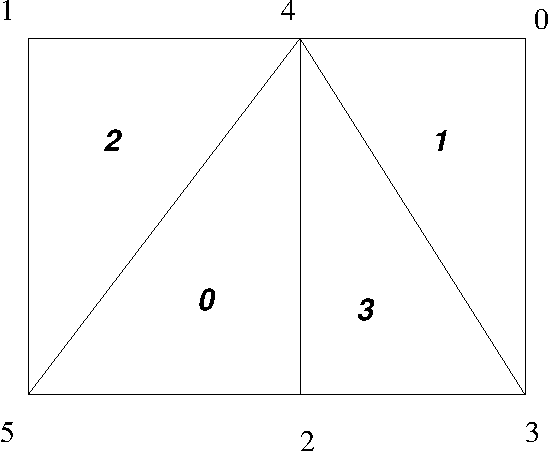
\includegraphics{usg.pdf}}
\caption{Numbering on Simple Unstructured Grid}
\label{fig_usg}
\end{figure}

This, of course, assumes that one has already distributed the grid (graph) information
among the processes. The details of this initial distribution is not important; it
could be simply determined by assigning to the first process the first $n_0$ nodes
from a file, the second process the next $ n_1$ nodes, etc.

For example, we demonstrate the form of the \lstinline{ia} and \lstinline{ja} for a triangular
grid where we

(1) partition by element (triangle)
\begin{itemize}
  \item Process 0: \lstinline{mlocal = 2}, \lstinline{n = 4}, \lstinline{ja = }\texttt{\{2,3, 3\}}, \lstinline{ia =} \texttt{\{0,2,3\}}
  \item Process 1: \lstinline{mlocal = 2}, \lstinline{n = 4}, \lstinline{ja = }\texttt{\{0,  0,1\}}, \lstinline{ia = }\texttt{\{0,1,3\}}
\end{itemize}
Note that elements are not connected to themselves and we only indicate edge connections
(in some contexts single vertex connections between elements may also be included). We use a
space above to denote the transition between rows in the matrix.

and (2) partition by vertex.
\begin{itemize}
  \item Process 0: \lstinline{mlocal = 3}, \lstinline{n = 6}, \lstinline{ja = }\texttt{\{3,4,  4,5, 3,4,5\}}, \lstinline{ia = }\texttt{\{0, 2, 4, 7\}}
  \item Process 1: \lstinline{mlocal = 3}, \lstinline{n = 6}, \lstinline{ja = }\texttt{\{0,2, 4, 0,1,2,3,5, 1,2,4\}}, \lstinline{ia = }\texttt{\{0, 3, 8, 11\}}.
\end{itemize}

Once the connectivity matrix has been created the following code will
generate the renumbering required for the new partition
\begin{lstlisting}
MatPartitioningCreate(MPI_Comm comm,MatPartitioning *part);
MatPartitioningSetAdjacency(MatPartitioning part,Mat Adj);
MatPartitioningSetFromOptions(MatPartitioning part);
MatPartitioningApply(MatPartitioning part,IS *is);
MatPartitioningDestroy(MatPartitioning *part); 
MatDestroy(Mat *Adj);
ISPartitioningToNumbering(IS is,IS *isg);
\end{lstlisting}
The resulting \lstinline{isg} contains for each local node the new global
number of that node. The resulting \lstinline{is} contains the new process number
that each local node has been assigned to.

Now that a new numbering of the nodes has been determined, one must
renumber all the nodes and migrate the grid information to the correct process.
The command
\begin{lstlisting}
AOCreateBasicIS(isg,NULL,&ao);
\end{lstlisting}
generates, see Section \ref{sec_ao}, an AO object that can be used in conjunction with the
\lstinline{is} and \lstinline{isg} to move the relevant grid information to the correct process
and renumber the nodes etc.
In this context, the new ordering is the ``application'' ordering so \lstinline{AOPetscToApplication()}
converts old global indices to new global indices and \lstinline{AOApplicationToPetsc()} converts new
global indices back to old global indices.

PETSc does not currently provide tools that completely manage the migration and
node renumbering, since it will be dependent on the particular data structure you
use to store the grid information and the type of grid information that you need
for your application. We do plan to include more support for this in the future,
but designing the appropriate general user interface and providing a scalable
implementation that can be used for a wide variety of different grids requires a
great deal of time.


% ------------------------------------------------------------------
\cleardoublepage
\chapter{KSP: Linear System Solvers} \sindex{linear system solvers}
\label{ch_ksp}

The object \lstinline{KSP} is the heart of PETSc, because it provides uniform and efficient access
to all of the package's linear system solvers, including parallel and sequential,
direct and iterative.
\lstinline{KSP} is intended for solving nonsingular systems of the form
\begin{equation}
 A x = b,
\label{eq_Ax=b}
\end{equation}
where $A$ denotes the matrix representation of a linear operator, $b$
is the right-hand-side vector, and $ x $ is the solution vector.  \lstinline{KSP}
uses the same calling sequence for both direct and iterative solution
of a linear system.  In addition, particular solution techniques and
their associated options can be selected at runtime.

The combination of a Krylov subspace method and a preconditioner is at
the center of most modern numerical codes for the iterative solution of
linear systems.  See, for example, \cite{fgn} for an overview of the theory
of such methods.  \lstinline{KSP} creates a simplified interface to the
lower-level \lstinline{KSP} and \lstinline{PC} modules within the PETSc package.  The \lstinline{KSP} package,
discussed in
Section~\ref{sec_ksp}, provides many popular Krylov
\sindex{Krylov subspace methods} subspace iterative methods;
the \lstinline{PC} module, described in Section~\ref{sec_pc}, includes a
variety of preconditioners.  Although both  \lstinline{KSP} and \lstinline{PC} can be used
directly, users should employ the interface of \lstinline{KSP}.

\section{Using KSP}
\label{sec_usingsles}

To solve a linear system with \lstinline{KSP}, one must first create a solver context
with the command
\begin{lstlisting}
KSPCreate(MPI_Comm comm,KSP *ksp);
\end{lstlisting}
Here \lstinline{comm} is the MPI communicator, and \lstinline{ksp} is the newly
formed solver context.
Before actually solving a linear system with \lstinline{KSP}, the user must call
the following routine to set the matrices associated with the linear
system:
\begin{lstlisting}
KSPSetOperators(KSP ksp,Mat Amat,Mat Pmat);
\end{lstlisting}
The argument \lstinline{Amat}, representing the matrix that defines the
linear system, is a symbolic place holder for any kind of matrix.
In particular, \lstinline{KSP} {\em does} support matrix-free methods.
\sindex{matrix-free methods}
The routine \lstinline{MatCreateShell()}
in Section~\ref{sec_matrixfree} provides further information regarding
matrix-free methods.
Typically, the matrix from which the
preconditioner is to be constructed, \lstinline{Pmat}, is the same as
the matrix that defines the linear system, \lstinline{Amat}; however,
occasionally these matrices differ (for instance, \sindex{preconditioning}
when a preconditioning matrix is obtained from a lower order method than
that employed to form the linear system matrix).

Much of the power of \lstinline{KSP} can be accessed through the single routine
\begin{lstlisting}
KSPSetFromOptions(KSP ksp);
\end{lstlisting}
This
routine accepts the options \trl{-h} and \trl{-help} as well as
any of the \lstinline{KSP} and \lstinline{PC} options discussed below.
To solve a linear system, one sets the rhs and solution vectors using
and executes the
command
\begin{lstlisting}
KSPSolve(KSP ksp,Vec b,Vec x);
\end{lstlisting}
where \lstinline{b} and \lstinline{x} respectively denote the right-hand-side and
solution vectors.  On return, the iteration number at which
the iterative process stopped
can be obtained using
\begin{lstlisting}
KSPGetIterationNumber(KSP ksp, PetscInt *its);
\end{lstlisting}
Note that this does not state that the method converged at this
iteration: it can also have reached the maximum number of iterations,
or have diverged.

Section~\ref{section_convergencetests} gives more details regarding
convergence testing. Note that multiple linear solves can be performed by
the same \lstinline{KSP} context. Once the \lstinline{KSP} context is no longer needed, it should be
destroyed with the command
\begin{lstlisting}
KSPDestroy(KSP *ksp);
\end{lstlisting}

The above procedure is sufficient for general use of the \lstinline{KSP} package.
One additional step is required for users who wish to customize certain
preconditioners (e.g., see Section~\ref{sec_bjacobi}) or to log certain
performance data using the PETSc profiling facilities (as discussed in
Chapter~\ref{ch_profiling}).
In this case, the user can optionally explicitly call
\begin{lstlisting}
KSPSetUp(KSP ksp)
\end{lstlisting}
before calling \lstinline{KSPSolve()} to perform any setup required for
the linear solvers.  The explicit call of this routine enables the
separate monitoring of any computations performed during the set up
phase, such as incomplete factorization for the ILU preconditioner.

The default solver within \lstinline{KSP} is restarted GMRES, preconditioned for
the uniprocess case with ILU(0), and for the multiprocess case
with the block Jacobi method (with one block per process, each of
which is solved with ILU(0)). A variety of other solvers
and options are also available.
To allow application programmers to set any of the preconditioner or
Krylov subspace options directly within the code, we provide routines
that extract the \lstinline{PC} and \lstinline{KSP} contexts,
\begin{lstlisting}
KSPGetPC(KSP ksp,PC *pc);
\end{lstlisting}
The application programmer can then directly call any of the \lstinline{PC} or \lstinline{KSP}
routines to modify the corresponding default options.

To solve a linear system with a direct solver (currently supported
by PETSc for sequential matrices, and by several external solvers through
PETSc interfaces (see Section~\ref{sec_externalsol})) one may use the options
\trl{-ksp_type} \trl{preonly} \trl{-pc_type} \trl{lu}
(see below).

By default, if a direct solver is used, the factorization is {\em not} done
in-place. This approach prevents the user from the unexpected surprise
of having a corrupted matrix after a linear solve. The routine
\lstinline{PCFactorSetUseInPlace()}, discussed below, causes factorization to
be done in-place.

\section{Solving Successive Linear Systems}

When solving multiple linear systems of the same size with the same
method, several options are available.  To solve successive linear
systems having the {\em same} preconditioner matrix (i.e., the same
data structure with exactly the same matrix elements) but different
right-hand-side vectors, the user should simply call \lstinline{KSPSolve()},
multiple times.  The preconditioner setup operations (e.g.,
factorization for ILU) will be done during the first call to \lstinline{KSPSolve()} only; such operations will {\em not} be repeated for
successive solves.

To solve successive linear systems that have {\em different}
preconditioner matrices (i.e., the matrix elements and/or the matrix
data structure change), the user {\em must} call
\lstinline{KSPSetOperators()} and \lstinline{KSPSolve()} for each solve.  See
Section~\ref{sec_usingsles} for a description of various flags for
\lstinline{KSPSetOperators()} that can save work for such cases.

\section{Krylov Methods}\sindex{Krylov subspace methods}
\label{sec_ksp}

The Krylov subspace methods accept a number of options, many of which
are discussed below.  First, to set the Krylov subspace method that is to
be used, one calls the command
\begin{lstlisting}
KSPSetType(KSP ksp,KSPType method);
\end{lstlisting}
The type can be one of \lstinline{KSPRICHARDSON}, \lstinline{KSPCHEBYSHEV}, \lstinline{KSPCG}, \lstinline{KSPGMRES},
\lstinline{KSPTCQMR}, \lstinline{KSPBCGS}, \lstinline{KSPCGS}, \lstinline{KSPTFQMR}, \lstinline{KSPCR}, \lstinline{KSPLSQR}, \lstinline{KSPBICG}, \lstinline{KSPPREONLY}. or others; see Table \ref{tab_kspdefaults} or the \lstinline{KSPType} man page for more. 
The \lstinline{KSP} method can also be set with the options database command
\trl{-ksp_type},
followed by one of the options \trl{richardson}, \trl{chebyshev}, \trl{cg}, \trl{gmres}, \trl{tcqmr},
\trl{bcgs}, \trl{cgs}, \trl{tfqmr}, \trl{cr}, \trl{lsqr}, \trl{bicg}, \trl{preonly.}, or others (see Table \ref{tab_kspdefaults} or the \lstinline{KSPType} man page) \findex{-ksp_type}
There are method-specific options:for instance, for the Richardson, Chebyshev,
and GMRES methods: \sindex{GMRES} \sindex{CG}
\begin{lstlisting}
KSPRichardsonSetScale(KSP ksp,PetscReal scale);
KSPChebyshevSetEigenvalues(KSP ksp,PetscReal emax,PetscReal emin);
KSPGMRESSetRestart(KSP ksp,PetscInt max_steps);
\end{lstlisting}
The default parameter values are \trl{damping_factor=1.0,
emax=0.01, emin=100.0}, and \trl{max_steps=30}. The GMRES
\sindex{restart} restart and Richardson damping factor
can also be set with the options \trl{-ksp_gmres_restart <n>}
and \trl{-ksp_richardson_scale <factor>}. \findex{-ksp_gmres_restart}
\findex{-ksp_richardson_scale}

The default technique for orthogonalization of the Hessenberg
matrix in GMRES is the
unmodified (classical) Gram-Schmidt method, which can be set \sindex{Gram-Schmidt}
with
\begin{lstlisting}
KSPGMRESSetOrthogonalization(KSP ksp,KSPGMRESClassicalGramSchmidtOrthogonalization);
\end{lstlisting}
or the options database \findex{-ksp_gmres_classicalgramschmidt}
command \trl{-ksp_gmres_classicalgramschmidt}.
By default this will {\em not} use iterative refinement to improve the
stability of the orthogonalization.
This can be changed with the option
\begin{lstlisting}
KSPGMRESSetCGSRefinementType(KSP ksp,KSPGMRESCGSRefinementType type)
\end{lstlisting}
or via the options database with
\begin{bashlisting}
-ksp_gmres_cgs_refinement_type none,ifneeded,always
\end{bashlisting}
\findex{-ksp_gmres_cgs_refinement_type}
The values for \lstinline{KSPGMRESCGSRefinementType()} are \lstinline{KSP_GMRES_CGS_REFINEMENT_NONE}, \findex{KSP_GMRES_CGS_REFINEMENT_NONE} \break
\lstinline{KSP_GMRES_CGS_REFINEMENT_IFNEEDED} and \lstinline{KSP_GMRES_CGS_REFINEMENT_ALWAYS}.
\findex{KSP_GMRES_CGS_REFINEMENT_IFNEEDED} \findex{KSP_GMRES_CGS_REFINEMENT_ALWAYS}

One can also use
modified Gram-Schmidt,
by using the orthogonalization routine \break
\lstinline{KSPGMRESModifiedGramSchmidtOrthogonalization()} or by using the command line option
\trl{-ksp_gmres_modifiedgramschmidt}. \findex{-ksp_gmres_modifiedgramschmidt}

For the conjugate gradient method with complex numbers, there are two
slightly different algorithms depending on whether the matrix is
Hermitian symmetric or truly symmetric (the default is to assume that
it is Hermitian symmetric). To indicate that it is symmetric, one uses the command
\findex{KSP_CG_SYMMETRIC}
\sindex{Hermitian matrix}
\begin{lstlisting}
KSPCGSetType(KSP ksp,KSPCGType KSP_CG_SYMMETRIC);
\end{lstlisting}
Note that this option is not valid for all matrices.

The LSQR algorithm does not involve a preconditioner; any preconditioner
set to work with the \lstinline{KSP} object is ignored if \lstinline{KSPLSQR} was selected.

By default, \lstinline{KSP} assumes an initial guess of zero by zeroing the initial
value for the solution vector that is given; this zeroing is done at the
call to \lstinline{KSPSolve()} (or \lstinline{KSPSolve()}). To use a nonzero
initial guess, the user {\em must} call
\begin{lstlisting}
KSPSetInitialGuessNonzero(KSP ksp,PetscBool flg);
\end{lstlisting}

\subsection{Preconditioning within KSP}
\label{sec_ksppc}
\sindex{preconditioning}

Since the rate of convergence of Krylov projection methods for a
particular linear system is strongly dependent on its spectrum,
preconditioning is typically used to alter the spectrum and hence
accelerate the convergence rate of iterative techniques.
Preconditioning can be applied to the system (\ref{eq_Ax=b}) by
\begin{equation}
(M_L^{-1} A M_R^{-1}) \, (M_R x) = M_L^{-1} b,
\label{eq_prec}
\end{equation}
where $ M_L$ and $ M_R $ indicate preconditioning matrices (or, matrices
from which the preconditioner is to be constructed).  If $ M_L = I $
in (\ref{eq_prec}), right preconditioning results, and the
residual of (\ref{eq_Ax=b}),
  \[ r \equiv b - Ax = b - A M_R^{-1} \, M_R x, \]
is preserved.  In contrast, the residual is altered for left
($ M_R = I $) and symmetric preconditioning, as given by
  \[ r_L \equiv M_L^{-1} b - M_L^{-1} A x = M_L^{-1} r. \]
By default, most KSP implementations use left preconditioning.
Some more naturally use other options, though. For instance, \lstinline{KSPQCG} defaults to use symmetric preconditioning and \lstinline{KSPFGMRES} uses right preconditioning by default. 
Right preconditioning can be activated for some methods by
using the options database command \trl{-ksp_pc_side right} or
calling the routine \findex{-ksp_pc_side}
\begin{lstlisting}
KSPSetPCSide(KSP ksp,PCSide PC_RIGHT);
\end{lstlisting}
Attempting to use right preconditioning for a method that
does not currently support it results in an error message of the form
\begin{outputlisting}
KSPSetUp_Richardson:No right preconditioning for KSPRICHARDSON
\end{outputlisting}

We summarize the defaults for the residuals used in KSP convergence
monitoring within Table~\ref{tab_kspdefaults}.  Details regarding 
specific convergence tests and monitoring routines are presented in
the following sections.  The preconditioned residual is used by
default for convergence testing of all left-preconditioned \lstinline{KSP}
methods. For the conjugate gradient, Richardson, and
Chebyshev methods the true residual can be used by
the options database command \trl{ksp_norm_type unpreconditioned } or by calling the routine
\begin{lstlisting}
KSPSetNormType(KSP ksp,KSP_NORM_UNPRECONDITIONED);
\end{lstlisting}

\begin{table}
\begin{center}
\begin{tabular}{lll}
& & {\bf Options}       \\
& & {\bf Database}      \\
{\bf Method}    &{\bf KSPType}  & {\bf Name}    \\
\hline
  Richardson                                                & \lstinline|KSPRICHARDSON| & \trl{richardson} \\
  Chebyshev                                                 & \lstinline|KSPCHEBYSHEV|  & \trl{chebyshev}  \\
  Conjugate Gradient \cite{hs:52}                           & \lstinline|KSPCG|         & \trl{cg}         \\
  \ Pipelined Conjugate Gradients                           & \lstinline|KSPPIPECG|     & \trl{pipecg}     \\
  \ Pipelined Conjugate Gradients (Gropp)                   & \lstinline|KSPGROPPCG|    & \trl{cgne}       \\
  \ Pipelined Conjugate Gradients with Residual Replacement & \lstinline|KSPPIPECGRR|   & \trl{pipecgrr}   \\
  \ Conjugate Gradients for the Normal Equations            & \lstinline|KSPCGNE|       & \trl{cgne}       \\
  \ Flexible Conjugate Gradients \cite{flexibleCG}          & \lstinline|KSPFCG|        & \trl{fcg}        \\
  \ Pipelined, Flexible Conjugate Gradient                  & \lstinline|KSPPIPEFCG|    & \trl{pipefcg}    \\
  \ Conjugate Gradients for Least Squares                   & \lstinline|KSPCGLS|       & \trl{cgls}       \\ 
  \ Conjugate Gradients with Constraint (1)                 & \lstinline|KSPNASH|       & \trl{nash}       \\
  \ Conjugate Gradients with Constraint (2)                 & \lstinline|KSPSTCG|       & \trl{stcg}       \\
  \ Conjugate Gradients with Constraint (3)                 & \lstinline|KSPGLTR|       & \trl{gltr}       \\
  \ Conjugate Gradients with Constraint (4)                 & \lstinline|KSPQCG|        & \trl{qcg}        \\
  BiConjugate Gradient                                      & \lstinline|KSPBICG|       & \trl{bicg}       \\
  BiCGSTAB \cite{v:92}                                      & \lstinline|KSPBCGS|       & \trl{bcgs}       \\
  \ Improved BiCGSTAB                                       & \lstinline|KSPIBCGS|      & \trl{ibcgs}      \\
  \ Flexible BiCGSTAB                                       & \lstinline|KSPFBCGS|      & \trl{fbcgs}      \\
  \ Flexible BiCGSTAB (variant)                             & \lstinline|KSPFBCGSR|     & \trl{fbcgsr}     \\
  \ Enhanced BiCGSTAB(L)                                    & \lstinline|KSPBCGSL|      & \trl{bcgsl}      \\
  Minimal Residual Method \cite{PaigeSaunders1975}          & \lstinline|KSPMINRES|     & \trl{minres}     \\
  Generalized Minimal Residual \cite{ss:86}                 & \lstinline|KSPGMRES|      & \trl{gmres}      \\
  \ Flexible Generalized Minimal Residual \cite{Saad1993}   & \lstinline|KSPFGMRES|     & \trl{fgmres}     \\
  \ Deflated Generalized Minimal Residual                   & \lstinline|KSPDGMRES|     & \trl{dgmres}     \\
  \ Pipelined Generalized Minimal Residual                  & \lstinline|KSPPGMRES|     & \trl{pgmres}     \\
  \ Pipelined, Flexible Generalized Minimal Residual        & \lstinline|KSPPIPEFGMRES| & \trl{pipefgmres} \\
  \ Generalized Minimal Residual with Accelerated Restart   & \lstinline|KSPLGMRES|     & \trl{lgmres}     \\
  Conjugate Residual \cite{eisenstat1983variational}        & \lstinline|KSPCR|         & \trl{cr}         \\
  \ Generalized Conjugate Residual                          & \lstinline|KSPGCR|        & \trl{gcr}        \\
  \ Pipelined Conjugate Residual                            & \lstinline|KSPPIPECR|     & \trl{pipecr}     \\
  \ Pipelined, Flexible Conjugate Residual                  & \lstinline|KSPPIPEGCR|    & \trl{pipegcr}    \\
  Conjugate Gradient Squared \cite{so:89}                   & \lstinline|KSPCGS|        & \trl{cgs}        \\
  Transpose-Free Quasi-Minimal Residual (1) \cite{f:93}     & \lstinline|KSPTFQMR|      & \trl{tfqmr}      \\
  Transpose-Free Quasi-Minimal Residual (2)                 & \lstinline|KSPTCQMR|      & \trl{tcqmr}      \\
  Least Squares Method                                      & \lstinline|KSPLSQR|       & \trl{lsqr}       \\
  Symmetric LQ Method \cite{PaigeSaunders1975}              & \lstinline|KSPSYMMLQ|     & \trl{symmlq}     \\
  TSIRM                                                     & \lstinline|KSPTSIRM|      & \trl{tsirm}      \\
  Python Shell                                              & \lstinline|KSPPYTHON|     & \trl{python}     \\
  Shell for no \lstinline|KSP| method                       & \lstinline|KSPPREONLY|    & \trl{preonly}    \\
\hline
\end{tabular}
\medskip \medskip
\end{center}
\caption{KSP Objects.}
\label{tab_kspdefaults}
\end{table}

Note: the bi-conjugate gradient method requires application of both the matrix and
its transpose plus the preconditioner and its transpose. Currently not all matrices
and preconditioners provide this support and thus the \lstinline{KSPBICG} cannot always
be used. \sindex{Bi-conjugate gradient}

\subsection{Convergence Tests}
\label{section_convergencetests}

The default convergence test, \lstinline{KSPConvergedDefault()}, is
based on the $l_2$-norm of the residual. Convergence
(or divergence) is decided by three quantities:
the decrease of the residual norm relative to the norm of the right hand side, \trl{rtol}, the absolute
size of the residual norm, \trl{atol}, and the relative increase in the
residual, \trl{dtol}.  Convergence is detected at iteration $ k $ if
\[  \| r_k \|_2 < {\rm max} ( \text{rtol} * \| b \|_2, \text{atol}), \]
where $r_k = b - A x_k$.  Divergence is detected if
\[  \| r_k \|_2 > \text{dtol} * \| b \|_2. \]
These parameters, as well as the maximum number of allowable iterations,
can be set with the routine
\begin{lstlisting}
KSPSetTolerances(KSP ksp,PetscReal rtol,PetscReal atol,PetscReal dtol,PetscInt maxits);
\end{lstlisting}
The user can retain the default value of any of these parameters by
specifying \lstinline{PETSC_DEFAULT} as the
corresponding tolerance; the
defaults are \lstinline{rtol=1e-5}, \lstinline{atol=1e-50},
\lstinline{dtol=1e5}, and \lstinline{maxits=1e4}.
These parameters can also be set from the options database with the 
commands \trl{-ksp_rtol} \trl{<rtol>}, \trl{-ksp_atol} \trl{<atol>}, \trl{-ksp_divtol} \trl{<dtol>},
\findex{-ksp_rtol} \findex{-ksp_atol} \findex{-ksp_divtol}
and \trl{-ksp_max_it} \trl{<its>}. \findex{-ksp_max_it}

In addition to providing an interface to a simple convergence test,
\lstinline{KSP} allows the application programmer the flexibility to provide
customized convergence-testing routines.  \sindex{convergence tests}
The user can specify a customized
routine with the command
\begin{lstlisting}
KSPSetConvergenceTest(KSP ksp,PetscErrorCode (*test)(KSP ksp,PetscInt it,PetscReal rnorm, KSPConvergedReason *reason,void *ctx),void *ctx,PetscErrorCode (*destroy)(void *ctx));
\end{lstlisting}
The final routine argument, \lstinline{ctx}, is an optional context for private
data for the user-defined convergence routine, \lstinline{test}.  Other
\lstinline{test} routine arguments are the iteration
number, \lstinline{it}, and the residual's $ l_2 $ norm, \lstinline{rnorm}.
The routine for detecting convergence, \lstinline{test}, should set \lstinline{reason} to
positive for convergence, 0 for no convergence, and negative for
failure to converge.  A full list of possible values for \lstinline{KSPConvergedReason} is given in \trl{include/petscksp.h}.
 You can use \lstinline{KSPGetConvergedReason()} after \lstinline{KSPSolve()} to see why
convergence/divergence was detected.

\subsection{Convergence Monitoring}
\label{sec_kspmonitor}

By default, the Krylov solvers run silently without displaying information
about the iterations. The user can indicate that the norms of the residuals
should be displayed by using \findex{-ksp_monitor}
\trl{-ksp_monitor} within the options database.
To display the residual norms in a graphical window (running under X Windows),
one should use \trl{-ksp_monitor_lg_residualnorm} \trl{[x,y,w,h]}, where either all or none of
the options must be specified. \findex{-ksp_monitor_lg_residualnorm}
Application programmers can also provide their own routines to perform
the monitoring by using the command
\begin{lstlisting}
KSPMonitorSet(KSP ksp,PetscErrorCode (*mon)(KSP ksp,PetscInt it,PetscReal rnorm,void *ctx),void *ctx,PetscErrorCode (*mondestroy)(void**));
\end{lstlisting}
The final routine argument, \lstinline{ctx}, is an optional context for private
data for the user-defined monitoring routine, \lstinline{mon}.  Other
\lstinline{mon} routine arguments are the iteration
number (\lstinline{it}) and the residual's $ l_2 $ norm (\lstinline{rnorm}).
A helpful routine within user-defined monitors is
\break\lstinline{PetscObjectGetComm((PetscObject)ksp,MPI_Comm *comm)}, which returns
in \lstinline{comm} \sindex{communicator} the
MPI communicator for the \lstinline{KSP} context.  See section ~\ref{sec_writing}
for more discussion of the use of MPI communicators within PETSc.

Several monitoring routines are supplied with PETSc,
including
\begin{lstlisting}
KSPMonitorDefault(KSP,PetscInt,PetscReal, void *);
KSPMonitorSingularValue(KSP,PetscInt,PetscReal,void *);
KSPMonitorTrueResidualNorm(KSP,PetscInt,PetscReal, void *);
\end{lstlisting}
The default monitor simply prints an estimate of the $l_2$-norm of the
residual at each iteration. The routine
\lstinline{KSPMonitorSingularValue()} is appropriate only for use with the conjugate
gradient method or GMRES, since it prints estimates of the extreme singular
values of the preconditioned operator at each iteration. Since
\lstinline{KSPMonitorTrueResidualNorm()} prints
the true residual at each iteration by
actually computing the residual using the formula $ r = b - Ax $, the routine
is slow and should be used only for testing or convergence studies,
not for timing. These monitors may be accessed with the command line options
\trl{-ksp_monitor}, \trl{-ksp_monitor_singular_value}, and \trl{-ksp_monitor_true_residual}.
\findex{-ksp_monitor} \findex{-ksp_monitor_singular_value} \findex{-ksp_monitor_true_residual}

To employ the default graphical monitor, one should use the
commands
\begin{lstlisting}
PetscDrawLG lg;
KSPMonitorLGResidualNormCreate(MPI_Comm comm,char *display,char *title,PetscInt x,PetscInt y,PetscInt w,PetscInt h,PetscDrawLG *lg);
KSPMonitorSet(KSP ksp,KSPMonitorLGResidualNorm,lg,0);
\end{lstlisting}
When no longer needed, the line graph should be destroyed
with the command
\begin{lstlisting}
PetscDrawLGDestroy(PetscDrawLG *lg);
\end{lstlisting}
The user can change aspects of the graphs with the \lstinline{PetscDrawLG*()} and
\lstinline{PetscDrawAxis*()} routines. \findex{PetscDrawAxis*()} \findex{PetscDrawLG*()}
One can also access this functionality from the options database
with the command \trl{-ksp_monitor_lg_residualnorm} \trl{[x,y,w,h]}. \findex{-ksp_monitor_lg_residualnorm},
where \trl{x, y, w, h} are the optional location and size of the window.

One can cancel hardwired monitoring routines for KSP at runtime with
\trl{-ksp_monitor_cancel}. \findex{-ksp_monitor_cancel}

Unless the Krylov method converges so that the residual norm is small,
say $10^{-10}$, many of the final digits printed with the \trl{-ksp_monitor}
option are meaningless. Worse, they are different on different
machines; due to different round-off rules used by, say, the IBM RS6000
and the Sun SPARC. This makes testing between different machines
difficult. The option \trl{-ksp_monitor_short} \findex{-ksp_monitor_short}
causes PETSc to print fewer of the digits of the residual norm
as it gets smaller; thus on most of the machines it will always
print the same numbers making cross system testing easier.

\subsection{Understanding the Operator's Spectrum}

Since the convergence of Krylov subspace methods depends strongly on
the spectrum (eigenvalues) of the preconditioned operator, PETSc has specific
routines for eigenvalue approximation via the Arnoldi or Lanczos iteration.
First, before the linear solve one must call
\begin{lstlisting}
KSPSetComputeEigenvalues(KSP ksp,PETSC_TRUE);
\end{lstlisting}
Then after the \lstinline{KSP} solve one calls
\begin{lstlisting}
KSPComputeEigenvalues(KSP ksp,PetscInt n,PetscReal *realpart,PetscReal *complexpart,PetscInt *neig);
\end{lstlisting}
Here, \lstinline{n} is the size of the two arrays and the eigenvalues are
inserted into those two arrays. \lstinline{neig} is the number of eigenvalues computed;
this number depends on the size of the Krylov space generated during the
linear system solution, for GMRES it is never larger than the restart parameter.
There is an additional routine
\begin{lstlisting}
KSPComputeEigenvaluesExplicitly(KSP ksp, PetscInt n,PetscReal *realpart,PetscReal *complexpart);
\end{lstlisting}
that is useful only for very small problems. It explicitly computes the
full representation of the preconditioned operator and calls LAPACK to
compute its eigenvalues. It should be only used for matrices of size up to
a couple hundred.  The \lstinline{PetscDrawSP*()} routines are very useful for
drawing scatter plots of the eigenvalues. \findex{PetscDrawSP*()}

The eigenvalues may also be computed and displayed graphically with the options
data base commands \trl{-ksp_plot_eigenvalues} and \trl{-ksp_plot_eigenvalues_explicitly}.  \findex{-ksp_plot_eigenvalues} \findex{-ksp_plot_eigenvalues_explicitly}
Or they can be dumped to the screen in ASCII text via
\trl{-ksp_compute_eigenvalues} and \trl{-ksp_compute_eigenvalues_explicitly}.
\findex{-ksp_compute_eigenvalues} \findex{-ksp_compute_eigenvalues_explicitly}
\sindex{eigenvalues} \sindex{spectrum} \sindex{Arnoldi} \sindex{Lanczos}

\subsection{Other KSP Options}

To obtain the solution vector and right hand side from a \lstinline{KSP}
context, one uses
\begin{lstlisting}
KSPGetSolution(KSP ksp,Vec *x);
KSPGetRhs(KSP ksp,Vec *rhs);
\end{lstlisting}
During the iterative process
the solution may not yet have been calculated or it may be stored in
a different location. To access the approximate solution during the
iterative process, one uses the command
\begin{lstlisting}
KSPBuildSolution(KSP ksp,Vec w,Vec *v);
\end{lstlisting}
where the solution is returned in \lstinline{v}. The user can optionally provide
a vector in \lstinline{w} as the location to store the vector; however, if
\lstinline{w} is \lstinline{NULL}, space allocated by PETSc in the \lstinline{KSP} context is
used. One should not destroy this vector. For certain \lstinline{KSP} methods,
(e.g., GMRES), the construction of the solution is expensive, while for many
others it doesn't evenrequire a vector copy.

Access to the residual is done in a similar way with the
command
\begin{lstlisting}
KSPBuildResidual(KSP ksp,Vec t,Vec w,Vec *v);
\end{lstlisting}
Again, for GMRES and certain other methods this is an expensive
operation.

\section{Preconditioners} \sindex{preconditioners}
\label{sec_pc}

As discussed in Section~\ref{sec_ksppc}, Krylov subspace methods are
typically used in conjunction with a preconditioner.
To employ a particular preconditioning method, the user can either select
it from the options database using input of the form
\trl{-pc_type <methodname>} or set the method with the
command \findex{-pc_type}
\begin{lstlisting}
PCSetType(PC pc,PCType method);
\end{lstlisting}
In Table~\ref{tab_pcdefaults} we summarize the basic
preconditioning methods supported in PETSc. See the \lstinline{PCType} manual page for a complete list. 
The \lstinline{PCSHELL} preconditioner uses a specific,
application-provided preconditioner.  The direct preconditioner, \lstinline{PCLU}~,
is, in fact, a direct solver for the linear system that uses LU
factorization. \lstinline{PCLU} is included as a preconditioner so that PETSc has a
consistent interface among direct and iterative linear solvers.

\begin{table}
\begin{center}
\begin{tabular}{lll}
{\bf Method}    &{\bf PCType}   & {\bf Options Database Name}\\
\hline
  Jacobi                                        & \lstinline|PCJACOBI|    & \trl{jacobi}\\
  Block Jacobi                                  & \lstinline|PCBJACOBI|   & \trl{bjacobi}\\
  SOR (and SSOR)                                & \lstinline|PCSOR|       & \trl{sor}\\
  SOR with Eisenstat trick                      & \lstinline|PCEISENSTAT| & \trl{eisenstat}\\
  Incomplete Cholesky                           & \lstinline|PCICC|       & \trl{icc}\\
  Incomplete LU                                 & \lstinline|PCILU|       & \trl{ilu}\\
  Additive Schwarz                              & \lstinline|PCASM|       & \trl{asm}\\
  Generalized Additive Schwarz                  & \lstinline|PCGASM|      & \trl{gasm}\\
  Algebraic Multigrid                           & \lstinline|PCGAMG|      & \trl{gamg}\\
  Balancing Domain Decomposition by Constraints & \lstinline|PCBDDC|      & \trl{bddc}\\
  Linear solver                                 & \lstinline|PCKSP|       & \trl{ksp} \\
  Combination of preconditioners                & \lstinline|PCCOMPOSITE| & \trl{composite} \\
\hline
  LU                                            & \lstinline|PCLU|        & \trl{lu}\\
  Cholesky                                      & \lstinline|PCCHOLESKY|  & \trl{cholesky}\\
  No preconditioning                            & \lstinline|PCNONE|      & \trl{none}\\
  Shell for user-defined \lstinline|PC|         & \lstinline|PCSHELL|     & \trl{shell}\\
\hline
\end{tabular}
\end{center}
  \caption{PETSc Preconditioners (partial list)}
\label{tab_pcdefaults}
\end{table}

Each preconditioner may have associated with it a set of options,
which can be set with routines and options database commands provided
for this purpose.  Such routine names and commands are all of the form
\trl{PC<TYPE><Option>} and \trl{-pc_<type>_<option> [value]}.  
A complete list can be found by consulting the \lstinline{PCType} manual page; we discuss
just a few in the sections below.

\subsection{ILU and ICC Preconditioners}
\label{sec_ilu_icc}

Some of the options for ILU preconditioner are
\begin{lstlisting}
PCFactorSetLevels(PC pc,PetscInt levels);
PCFactorSetReuseOrdering(PC pc,PetscBool  flag);
PCFactorSetDropTolerance(PC pc,PetscReal dt,PetscReal dtcol,PetscInt dtcount);
PCFactorSetReuseFill(PC pc,PetscBool  flag);
PCFactorSetUseInPlace(PC pc,PetscBool flg); 
PCFactorSetAllowDiagonalFill(PC pc,PetscBool flg);
\end{lstlisting}

When repeatedly solving linear systems with the same \lstinline{KSP}
context, one can reuse some information  computed
during the first linear solve.
In particular, \lstinline{PCFactorSetReuseOrdering()} causes the ordering  (for example, set with
\trl{-pc_factor_mat_ordering_type} \trl{order}) computed in the first factorization to be reused
for later factorizations. \sindex{orderings}
%\lstinline{ PCFactorDTSetReuseFill()} causes the
%fill computed during the first drop tolerance factorization to be reused
%in later factorizations.
\lstinline{PCFactorSetUseInPlace()} is often used with
\lstinline{PCASM} or \lstinline{PCBJACOBI} when zero fill is used, since it reuses the
matrix space to store the incomplete factorization it saves memory and
copying time. Note that in-place factorization is not appropriate with
any ordering besides natural and cannot be used with the drop tolerance
factorization. These options may be set in the database with
\begin{tightitemize}
\item \trl{-pc_factor_levels <levels>}
\item \trl{-pc_factor_reuse_ordering}
%   tr\l{-pc_factor_drop_tolerance <dt>,<dtcol>,<dtcount>}
\item \trl{-pc_factor_reuse_fill}
\item \trl{-pc_factor_in_place}
\item \trl{-pc_factor_nonzeros_along_diagonal}
\item \trl{-pc_factor_diagonal_fill
}
\end{tightitemize}
\findex{-pc_factor_levels} \findex{-pc_factor_reuse_ordering}
%\findex{-pc_factor_drop_tolerance}
\findex{-pc_factor_reuse_fill}
\findex{-pc_factor_in_place} \findex{-pc_factor_nonzeros_along_diagonal}
\findex{-pc_factor_diagonal_fill}

See Section~\ref{sec_symbolfactor} for information on preallocation
of memory for anticipated fill during factorization.
By alleviating the considerable overhead for dynamic memory allocation,
such tuning can significantly enhance performance.

% --------------------------------------------------------------------
\label{sec_pcfactor}
PETSc supports incomplete factorization preconditioners for several matrix
types for sequential matrices (for example \lstinline{MATSEQAIJ}, \lstinline{MATSEQBAIJ}, and \lstinline{MATSEQSBAIJ}).\sindex{ILU, parallel}\sindex{ICC, parallel}


% --------------------------------------------------------------------

\subsection{SOR and SSOR Preconditioners}

PETSc only provides only a sequential SOR preconditioner; it can only be used with sequential
matrices or as the subblock preconditioner when using block Jacobi or
ASM preconditioning (see below).

The options for SOR \sindex{SSOR} \sindex{SOR} \sindex{relaxation}
preconditioning with \lstinline{PCSOR} are
\begin{lstlisting}
PCSORSetOmega(PC pc,PetscReal omega);
PCSORSetIterations(PC pc,PetscInt its,PetscInt lits);
PCSORSetSymmetric(PC pc,MatSORType type);
\end{lstlisting}
The
first of these commands sets the relaxation factor for successive
over (under) relaxation.  The second command sets the number of inner
iterations \trl{its} and local iterations \trl{lits}
(the number of smoothing sweeps on a
process before doing a ghost point update from the other processes)
to use between steps of the
Krylov space method. The total number of SOR sweeps is given by \trl{its*lits}.
The third command sets the kind of SOR sweep,
where the argument \lstinline{type} can be one of \lstinline{SOR_FORWARD_SWEEP},
\lstinline{SOR_BACKWARD_SWEEP} or \lstinline{SOR_SYMMETRIC_SWEEP}, the default
being \lstinline{SOR_FORWARD_SWEEP}. Setting the type to be \lstinline{SOR_SYMMETRIC_SWEEP} produces the SSOR method.  In addition,
each process can locally and independently perform the specified
variant of SOR with the types \lstinline{SOR_LOCAL_FORWARD_SWEEP},
\lstinline{SOR_LOCAL_BACKWARD_SWEEP}, and \lstinline{SOR_LOCAL_SYMMETRIC_SWEEP}.
These \findex{SOR_FORWARD_SWEEP} \findex{SOR_BACKWARD_SWEEP}
variants \findex{SOR_SYMMETRIC_SWEEP} \findex{SOR_LOCAL_FORWARD_SWEEP}
can \findex{SOR_LOCAL_BACKWARD_SWEEP} \findex{SOR_LOCAL_SYMMETRIC_SWEEP}
also be set with the options \trl{-pc_sor_omega <omega>},
\trl{-pc_sor_its <its>},  \trl{-pc_sor_lits <lits>},
\trl{-pc_sor_backward},  \trl{-pc_sor_symmetric},
\trl{-pc_sor_local_forward},  \trl{-pc_sor_local_backward}, and
\trl{-pc_sor_local_symmetric}.
\findex{-pc_sor_omega} \findex{-pc_sor_its}
\findex{-pc_sor_backward} \findex{-pc_sor_symmetric}
\findex{-pc_sor_local_forward} \findex{-pc_sor_local_backward}
\findex{-pc_sor_local_symmetric}

The Eisenstat trick \cite{eisenstat81} \sindex{Eisenstat trick} for SSOR preconditioning
can be employed with the method \lstinline{PCEISENSTAT}
(\trl{-pc_type} \trl{eisenstat}).
By using both left and right preconditioning of the linear system,
this variant of SSOR requires about half of the floating-point operations
for conventional SSOR. The option
\trl{-pc_eisenstat_no_diagonal_scaling})
(or the routine \lstinline{PCEisenstatSetNoDiagonalScaling()})
turns off diagonal scaling in conjunction with Eisenstat SSOR method, while
the option \trl{-pc_eisenstat_omega <omega>} (or the routine
\lstinline{PCEisenstatSetOmega(PC pc,PetscReal omega)})
sets the SSOR relaxation coefficient, \trl{omega}, as discussed above.
\findex{-pc_eisenstat_omega}

%------------------------------------------------------------------
\subsection{LU Factorization}
\label{sec_factorization}

The LU preconditioner provides several options.  The first, given by
the \sindex{direct solver}
command  \sindex{in-place solvers}
\begin{lstlisting}
PCFactorSetUseInPlace(PC pc,PetscBool flg);
\end{lstlisting}
causes the factorization to be performed in-place and hence
destroys the original matrix.  The options database variant of
this command is \trl{-pc_factor_in_place}. \findex{-pc_factor_in_place}
Another direct preconditioner option is selecting the ordering
of equations with the command \findex{-pc_factor_mat_ordering_type} \sindex{orderings}
   \trl{-pc_factor_mat_ordering_type <ordering>}.
The possible orderings are
\begin{itemize}
\item \lstinline{MATORDERINGNATURAL} - Natural
\item \lstinline{MATORDERINGND} - Nested Dissection
\item \lstinline{MATORDERING1WD} - One-way Dissection
\item \lstinline{MATORDERINGRCM} - Reverse Cuthill-McKee
\item \lstinline{MATORDERINGQMD} - Quotient Minimum Degree
\end{itemize}
\findex{MATORDERINGNATURAL} \findex{MATORDERINGND} \findex{MATORDERING1WD}
\findex{MATORDERINGRCM} \findex{MATORDERINGQMD} \sindex{nested dissection}
\sindex{one-way dissection} \sindex{reverse Cuthill-McKee}
\sindex{quotient minimum degree} \findex{-pc_factor_mat_ordering_type}
These orderings can also be set through the options database by specifying
one of the following:  \trl{-pc_factor_mat_ordering_type} \trl{natural}, or \trl{nd}, or  \trl{1wd}, or \trl{rcm}, or \trl{qmd}.
In addition, see \lstinline{MatGetOrdering()}, discussed in Section~\ref{sec_matfactor}.

The sparse LU factorization provided in PETSc does not perform pivoting for
numerical stability (since they are designed to preserve nonzero
structure), and thus occasionally a LU factorization will fail with a zero
pivot when, in fact, the matrix is non-singular. The option
\trl{-pc_factor_nonzeros_along_diagonal <tol>} \findex{-pc_factor_nonzeros_along_diagonal}
will often help eliminate the zero pivot, by preprocessing the
column ordering to remove small values from the diagonal. Here, \trl{tol}
is an optional tolerance to decide if a value is nonzero; by default it
is~\trl{1.e-10}.

In addition, Section~\ref{sec_symbolfactor} provides information on
preallocation of memory for anticipated fill during factorization.
Such tuning can significantly enhance performance, since it
eliminates the considerable overhead for dynamic memory allocation.

%----------------------------------------------------------------------
\subsection{Block Jacobi and
            Overlapping Additive Schwarz Preconditioners}
\label{sec_bjacobi}

\sindex{Jacobi} \sindex{block Jacobi}
\sindex{block Gauss-Seidel} \sindex{ASM} \sindex{overlapping Schwarz}
The block Jacobi and overlapping additive Schwarz methods in PETSc are
supported in parallel; however, only the uniprocess
version of the block Gauss-Seidel method is currently in place.
By default, the PETSc implementations of these methods
employ ILU(0) factorization on each individual block (that is, the default solver on each
subblock is \lstinline{PCType=PCILU}, \lstinline{KSPType=KSPPREONLY}); 
the user can set alternative linear solvers via the options
\findex{-sub_ksp_type} \findex{-sub_pc_type}
\trl{-sub_ksp_type} and \trl{-sub_pc_type}. In fact, all of the \lstinline{KSP}
and \lstinline{PC} options can be applied to the subproblems by inserting the prefix
\trl{-sub_} at the beginning of the option name. \sindex{local linear solves}
These options database commands set the particular options for {\em all}
of the blocks within the global problem.  In addition, the routines
\begin{lstlisting}
PCBJacobiGetSubKSP(PC pc,PetscInt *n_local,PetscInt *first_local,KSP **subksp);
PCASMGetSubKSP(PC pc,PetscInt *n_local,PetscInt *first_local,KSP **subksp);
\end{lstlisting}
extract the \lstinline{KSP} context for each local
block.  The argument \lstinline{n_local} is the number of blocks on the
calling process, and \lstinline{first_local} indicates the global number
of the first block on the process. The blocks are numbered
successively by processes from zero through $b_g-1$,
where $b_g$ is the number of global blocks.
The array of \lstinline{KSP} contexts for the local blocks is given by \trl{subksp}.
This mechanism enables the user to set different solvers for the
various blocks.  To set the appropriate data structures, the
user {\em must} explicitly call \lstinline{KSPSetUp()}
before calling \lstinline{PCBJacobiGetSubKSP()} or
\lstinline{PCASMGetSubKSP(}).
For further details, see the
examples \href{http://www.mcs.anl.gov/petsc/petsc-current/src/ksp/ksp/examples/tutorials/ex7.c.html}{\trl{$PETSC_DIR/src/ksp/ksp/examples/tutorials/ex7.c}}
or \href{http://www.mcs.anl.gov/petsc/petsc-current/src/ksp/ksp/examples/tutorials/ex7.c.html}{\trl{$PETSC_DIR/src/ksp/ksp/examples/tutorials/ex8.c}}.

The block Jacobi, block Gauss-Seidel, and additive Schwarz
preconditioners allow the user
to set the number of blocks into which the problem is divided.  The
options database commands to set this value are \trl{-pc_bjacobi_blocks} \trl{n}
and \trl{-pc_bgs_blocks} \trl{n}, and, within a program, the corresponding routines
are \sindex{block Jacobi} \sindex{block Gauss-Seidel}
\findex{-pc_bjacobi_blocks} \findex{-pc_bgs_blocks}
\begin{lstlisting}
PCBJacobiSetTotalBlocks(PC pc,PetscInt blocks,PetscInt *size);
PCASMSetTotalSubdomains(PC pc,PetscInt n,IS *is,IS *islocal);
PCASMSetType(PC pc,PCASMType type);
\end{lstlisting}
The
optional argument \lstinline{size} is an array indicating the size of
each block. Currently, for certain parallel matrix formats, only a
single block per process is supported. However, the \lstinline{MATMPIAIJ} and
\lstinline{MATMPIBAIJ} formats
support the use of general blocks as long as no blocks are shared
among processes. The \lstinline{is} argument contains the index sets that
define the subdomains.

The object \lstinline{PCASMType} is one of \lstinline{PC_ASM_BASIC},
\lstinline{PC_ASM_INTERPOLATE}, \lstinline{PC_ASM_RESTRICT}, or\break \lstinline{PC_ASM_NONE}
and may also be set with the options database
\trl{-pc_asm_type} \trl{[basic}, \trl{interpolate}, \trl{restrict}, \trl{none]}.
\findex{-pc_asm_type}  \findex{PC_ASM_BASIC}
\findex{PC_ASM_RESTRICT} \findex{PC_ASM_INTERPOLATE} \findex{PC_ASM_NONE}
The type \lstinline{PC_ASM_BASIC} (or \trl{-pc_asm_type} \trl{basic}) corresponds to the
standard additive Schwarz method that uses the full restriction and
interpolation operators.
The type \lstinline{PC_ASM_RESTRICT} (or \trl{-pc_asm_type} \trl{restrict}) uses a full
restriction operator, but during the interpolation process ignores the off-process
values.
Similarly, \lstinline{PC_ASM_INTERPOLATE} (or \trl{-pc_asm_type} \trl{interpolate}) uses a limited
restriction process in conjunction with a full interpolation, while
\lstinline{PC_ASM_NONE} (or \trl{-pc_asm_type} \trl{none}) ignores off-process values
for both restriction and interpolation.
The ASM types with limited restriction or interpolation were suggested by
Xiao-Chuan Cai and Marcus Sarkis \cite{cs97a}.  \sindex{Cai, Xiao-Chuan}  \sindex{Sarkis, Marcus}
\lstinline{PC_ASM_RESTRICT} is the PETSc default, as it saves substantial communication
and for many problems has the added benefit of requiring fewer iterations for convergence
than the standard additive Schwarz method.

The user can also set the number of blocks and sizes on a per-process
basis with the commands
\begin{lstlisting}
PCBJacobiSetLocalBlocks(PC pc,PetscInt blocks,PetscInt *size);
PCASMSetLocalSubdomains(PC pc,PetscInt N,IS *is,IS *islocal);
\end{lstlisting}

For the ASM preconditioner one can use the following command to set
the overlap to compute in constructing the subdomains.
\begin{lstlisting}
PCASMSetOverlap(PC pc,PetscInt overlap);
\end{lstlisting}
The overlap defaults to 1, so if one desires that no additional
overlap be computed beyond what may have been set with a call to \lstinline{PCASMSetTotalSubdomains()} or \lstinline{PCASMSetLocalSubdomains()}, then
\trl{overlap} must be set to be 0.  In particular, if one does {\em
not} explicitly set the subdomains in an application code, then all
overlap would be computed internally by PETSc, and using an overlap of
0 would result in an ASM variant that is equivalent to the block
Jacobi preconditioner.  Note that one can define initial index sets
\trl{is} with {\em any} overlap via \lstinline{PCASMSetTotalSubdomains()} or
\lstinline{PCASMSetLocalSubdomains()}; the routine \lstinline{PCASMSetOverlap()}
merely allows PETSc to extend that overlap further if desired.

\lstinline{PCGASM} is an experimental generalization of \lstinline{PCASM} that allows the user to specify subdomains
that span multiple MPI ranks.  This can be useful for problems where small subdomains result
in poor convergence.  To be effective, the multirank subproblems must be solved using a sufficient
strong subsolver, such as LU, for which \trl{SuperLU_DIST} or a similar parallel
direct solver could be used; other choices may include a multigrid solver on the subdomains.

The interface for \lstinline{PCGASM} is similar to that of \lstinline{PCASM}. In particular,
\lstinline{PCGASMType} is one of \lstinline{PC_GASM_BASIC},
\lstinline{PC_GASM_INTERPOLATE}, \lstinline{PC_GASM_RESTRICT}, \lstinline{PC_GASM_NONE}.
These options have the same meaning as with \lstinline{PCASM}
and may also be set with the options database
\trl{-pc_gasm_type} \trl{[basic}, \trl{interpolate}, \trl{restrict}, \trl{none]}.
\findex{-pc_gasm_type}  \findex{PC_GASM_BASIC}
\findex{PC_GASM_RESTRICT} \findex{PC_GASM_INTERPOLATE} \findex{PC_GASM_NONE}

Unlike \lstinline{PCASM}, however, \lstinline{PCGASM} allows the user to define subdomains that span multiple MPI ranks.
The simplest way to do this is using a call to \lstinline{PCGASMSetTotalSubdomains(PC pc,PetscPetscInt N)} with the
total number of subdomains \lstinline{N} that is smaller than the MPI communicator \lstinline{size}. In this case
\lstinline{PCGASM} will coalesce \lstinline{size/N} concecutive single-rank subdomains into a single multi-rank subdomain.
The single-rank subdomains contain the degrees of freedom corresponding to the locally-owned rows of the
\lstinline{PCGASM} preconditioning matrix -- these are the subdomains \lstinline{PCASM} and \lstinline{PCGASM} use by default.

Each of the multirank subdomain subproblems is defined on the subcommunicator that contains the coalesced
\lstinline{PCGASM} ranks.  In general this might not result in a very good subproblem if the single-rank problems
corresponding to the coalesced ranks are not very strongly connected.  In the future this will be addressed
with a hierarchical partitioner that generates well-connected coarse subdomains first before subpartitioning
them into the single-rank subdomains.

In the meantime the user can provide his or her own multi-rank subdomains by calling\break \lstinline{PCGASMSetSubdomains(PC,IS[],IS[])}
where each of the \lstinline{IS} objects on the list defines the inner (without the overlap) or the outer (including the overlap)
subdomain on the subcommunicator of the \lstinline{IS} object.  A helper subroutine \lstinline{PCGASMCreateSubdomains2D()} is similar
to PCASM's but is capable of constructing multi-rank subdomains that can be then used with \lstinline{PCGASMSetSubdomains()}.
An alternative way of creating multi-rank subdomains is by using the underlying DM object, if it is capable of generating
such decompositions via \lstinline{DMCreateDomainDecomposition()}. Ordinarily the decomposition specified by the user via
\lstinline{PCGASMSetSubdomains()} takes precedence, unless \lstinline{PCGASMSetUseDMSubdomains()} instructs \lstinline{PCGASM} to prefer \lstinline{DM}-created
decompositions.

Currently there is no support for increasing the overlap of multi-rank subdomains via\break \lstinline{PCGASMSetOverlap()} -- this
functionality works only for subdomains that fit within a single MPI rank, exactly as in \lstinline{PCASM}.

Examples of the described PCGASM usage can be found in \href{http://www.mcs.anl.gov/petsc/petsc-current/docs/manualpages/PC/PCGASM.html}{\trl{${PETSC_DIR}/src/ksp/ksp/examples/tutorials/ex62.c}}.
In particular, \trl{runex62_superlu_dist}
illustrates the use of \trl{SuperLU_DIST} as the subdomain solver on
coalesced multi-rank subdomains. The \trl{runex62_2D_*} examples illustrate the use of \lstinline{PCGASMCreateSubdomains2D()}.


%----------------------------------------------------------------------
\subsection{Algebraic Multigrid (AMG) Preconditioners}
\label{sec_amg}

PETSc has a native algebraic multigrid preconditioner \lstinline{PCGAMG} -- {\it gamg} -- and interfaces to two
external AMG packages: {\it hypre} and {\it ML}.
{\it Hypre}  is relatively monolithic in that a PETSc matrix is into a hypre matrix and then {\it hypre} is called to do the entire solve.
{\it ML} is more modular in that PETSc only has {\it ML} generate the coarse grid spaces (columns of the prolongation operator), which is core of an AMG method, and then constructs a \lstinline{PCMG} with Galerkin coarse grid operator construction. 
GAMG is designed from the beginning to be modular, to allow for new components to be added easily and also populates a multigrid preconditioner \lstinline{PCMG} so generic multigrid parameters are used.
PETSc provides a fully supported (smoothed) aggregation AMG, (\trl{-pc_type gamg -pc_gamg_type agg} or  \lstinline{PCSetType(pc,PCGAMG)} and \lstinline{PCGAMGSetType(pc,PCGAMGAGG)}, as well as reference implementations of a classical AMG method (\trl{-pc_gamg_type classical}), a hybrid geometric AMG method (\trl{-pc_gamg_type geo}), and a 2.5D AMG method DofColumns \cite{IsaacStadlerGhattas2015}.
GAMG does require the use of (MPI)AIJ matrices.
For instance, BAIJ matrices are not supported.
One can use AIJ instead of BAIJ without changing any code other than the constructor (or the \trl{-mat_type} from the command line).
For instance, \lstinline{MatSetValuesBlocked} works with AIJ matrices.

GAMG provides unsmoothed aggregation (\trl{-pc_gamg_agg_nsmooths 0}) and smoothed aggregation (\trl{-pc_gamg_agg_nsmooths 1} or \lstinline{PCGAMGSetNSmooths(pc,1)}).
Smoothed aggregation is recommended for symmetric positive definite
systems.
Unsmoothed aggregation can be useful for asymmetric
problems and problems where highest eigen estimates are problematic. 
If poor convergence rates are observed using the smoothed version one can test unsmoothed aggregation.
AMG methods requires knowledge of the number of degrees of
freedom per vertex, the default is one (a scalar problem).
Vector problems like elasticity should set the block size of the matrix appropriately with \trl{-mat_block_size bs}  or \lstinline{MatSetBlockSize(mat,bs)}.
Equations must be ordered in ``vertex-major'' ordering (e.g., $x_1,y_1,z_1,x_2,y_2,...$).

Smoothed aggregation requires an explicit representation of the (near) null space of the operator for optimal performance.
One can provide an orthonormal set of null space vectors with \lstinline{MatSetNearNullSpace()}.
The vector of all ones is the default, for each variable given by the block size (e.g., the translational rigid  body modes).
For elasticity, where rotational rigid body modes are required to complete the near null space you can use \lstinline{MatNullSpaceCreateRigidBody()} to create the null space vectors and then \lstinline{MatSetNearNullSpace()}.

There are several options to provide parameters to the coarsening algorithm and parallel data layout.
Run a code that uses GAMG with \trl{-help} to get full listing of GAMG parameters with short parameter descriptions.

{\bf Trouble shooting algebraic multigrid methods:}  
If {\it GAMG}, {\it ML}, or {\it hypre} does not perform well the first thing to try is one of 
the other methods. Often the default parameters or just the strengths of different algorithms can fix performance problems or provide useful information to guide further debugging.

There are several sources of poor performance of
AMG solvers and often special purpose methods must be developed to
achieve the full potential of multigrid.
To name just a few sources of performance degradation that
may not be fixed with parameters in PETSc currently: non-elliptic
operators, curl/curl operators, highly stretched grids or highly anisotropic problems,
large jumps in material coefficients with complex geometry (AMG is
particularly well suited to jumps in coefficients but it is not a
perfect solution), highly incompressible elasticity, not to mention
ill-posed problems, and many others. For Grad-Div and Curl-Curl operators,
you may want to try the Auxilary Maxwell Space (AMS, \trl{-pc_type hypre -pc_hypre_set_type ams})
or the Auxilary Divergence Space (ADS, \trl{-pc_type hypre -pc_hypre_set_type ads}) solvers.
These solvers need some additional information on the underlying mesh;
specifically, AMS needs the discrete gradient operator, which can be specified via
\lstinline{PCHYPRESetDiscreteGradient()}. In addition to the discrete gradient, ADS also needs the
specification of the discrete curl operator, which can be set using \lstinline{PCHYPRESetDiscreteCurl()}.

{\bf I am converging slowly, what do I do?}
AMG methods are sensitive to coarsening rates and methods; for GAMG
use \trl{-pc_gamg_threshold <x>} to regulate coarsening rates and
PCGAMGSetThreshold, higher values decrease coarsening rate.
Squaring the graph is the second mechanism for increasing coarsening
rate.
Use \trl{-pc_gamg_square_graph <N>,}, or \lstinline{PCGAMGSetSquareGraph(pc,N)}, to square the graph on the
finest N levels.  A high threshold (e.g., $x=0.08$) will result in an
expensive but potentially powerful preconditioner, and a low threshold
(e.g., $x=0.0$) will result in faster coarsening, fewer levels,
cheaper solves, and generally worse convergence rates.

One can run with \trl{-info} and grep for ``GAMG'' to get some statistics on each
level, which can be used to see if you are coarsening at an
appropriate rate.  With smoothed aggregation you generally want to
coarse at about a rate of 3:1 in each dimension.  Coarsening too slow
will result in large numbers of non-zeros per row on coarse grids
(this is reported).  The number of non-zeros can go up very high, say
about 300 (times the degrees-of-freedom per vertex) on a 3D hex mesh.
One can also look at the grid complexity, which is also reported (the ration of the total number of matrix entries for all levels to the number of matrix entries on the fine level).  
Grid complexity should be well under 2.0 and preferably around $1.3$ or lower.  If
convergence is poor and the Galerkin coarse grid construction is much
smaller than the time for each solve then one can safely decrease the
coarsening rate.  \trl{-pc_gamg_threshold} $0.0$ is the simplest and most robust
option, and is recommended if poor
convergence rates are observed, at least until the source of the
problem is discovered.
In conclusion, if convergence is slow then decreasing the coarsening rate (increasing the threshold) should be tried.

{\bf A note on Chebyshev smoothers.} Chebyshev solvers are attractive as multigrid smoothers because they can target a specific interval of the spectrum which is the purpose of a smoother.
The spectral bounds for Chebyshev solvers are simple to compute because they rely on the highest eigenvalue of your (diagonally preconditioned) operator, which is conceptually simple to compute.
However, if this highest eigenvalue estimate is not accurate (too low) then the solvers can fail with and indefinite preconditioner message.
One can run with \trl{-info} and grep for ``GAMG'' to get these estimates or use \trl{-ksp_view}.
These highest eigenvalues are generally between 1.5-3.0.
For symmetric positive definite systems CG is a better eigenvalue estimator \trl{-mg_levels_esteig_ksp_type cg}.
Indefinite matrix messages are often caused by bad Eigen estimates.
Explicitly damped Jacobi or Krylov smoothers can provide an alternative to Chebyshev and {\it hypre} has alternative smoothers.

{\bf Now am I solving alright, can I expect better?}
If you find that you are getting nearly on digit in reduction
of the residual per iteration and are using a modest number of point
smoothing steps (e.g., 1-4 iterations of SOR), then you may be fairly
close to textbook multigrid efficiency.  Although you also need to
check the setup costs.  This can be determined by running with
\trl{-log_view} and check that the time for the Galerkin coarse grid
construction (\lstinline{MatPtAP}) is not (much) more than the time spent in each
solve (\lstinline{KSPSolve}).  If the \lstinline{MatPtAP} time is too large then one can increase the
coarsening rate by decreasing the threshold and squaring the coarsening
graph (\trl{-pc_gamg_square_graph <N>}, squares the graph on the finest N levels).
Likewise if your \lstinline{MatPtAP} time is small and your convergence rate is not ideal then you could decrease the coarsening rate.

PETSc's AMG solver is constructed as a framework for developers to
easily add AMG capabilities, like a new AMG methods or anAMG component like a matrix
triple product. Contact us directly if you are interested in contributing.

%----------------------------------------------------------------------
\subsection{Balancing Domain Decomposition by Constraints}

PETSc provides the Balancing Domain Decomposition by Constraints (BDDC) method for preconditioning
parallel finite element problems stored in unassembled format (see \lstinline{MATIS}). BDDC is a 2-level
non-overlapping domain decomposition method which can be easily adapted to different problems
and discretizations by means of few user customizations. The application of the preconditioner to a vector consists
in the static condensation of the residual at the interior of the subdomains by means of local Dirichet solves, followed by an
additive combination of Neumann local corrections and the solution of a global coupled coarse problem. 
Command line options for the underlying \lstinline{KSP} objects are prefixed by \trl{-pc_bddc_dirichlet}, \trl{-pc_bddc_neumann},
and \trl{-pc_bddc_coarse} respectively.

The current implementation supports any kind of linear system, and assumes a one-to-one mapping between subdomains and
MPI processes. Complex numbers are supported as well. For non-symmetric problems, use the runtime option \trl{-pc_bddc_symmetric 0}.

Unlike conventional non-overlapping methods that iterates just on the degrees of freedom at the interface between subdomain,
\lstinline{PCBDDC} iterates on the whole set of degrees of freedom, allowing the use of approximate subdomain solvers.
When using approximate solvers, the command line switches \trl{-pc_bddc_dirichlet_approximate} and/or \trl{-pc_bddc_neumann_approximate} should be used to inform \lstinline{PCBDDC}.
If any of the local problems is singular, the nullspace of the local operator should be attached to the local matrix via \lstinline{MatSetNullSpace()}.

At the basis of the method there's the analysis of the connected components of the interface for the detection of vertices,
edges and faces equivalence classes. Additional information on the degrees of freedom can be supplied to \lstinline{PCBDDC} by using
the following functions: 
\begin{tightitemize}
\item \lstinline{PCBDDCSetDofsSplitting()}
\item \lstinline{PCBDDCSetLocalAdjacencyGraph()}
\item \lstinline{PCBDDCSetPrimalVerticesLocalIS()}
\item \lstinline{PCBDDCSetNeumannBoundaries()}
\item \lstinline{PCBDDCSetDirichletBoundaries()}
\item \lstinline{PCBDDCSetNeumannBoundariesLocal()}
\item \lstinline{PCBDDCSetDirichletBoundariesLocal()}
\end{tightitemize}

Crucial for the convergence of the iterative process is the specification of the primal constraints to be imposed at the interface
between subdomains. \lstinline{PCBDDC} uses by default vertex continuities and edge arithmetic averages, which are enough for the three-dimensional
Poisson problem with constant coefficients. The user can switch on and off the usage of vertices, edges or face constraints by using the command line
switches \trl{-pc_bddc_use_vertices}, \trl{-pc_bddc_use_edges}, \trl{-pc_bddc_use_faces}. A customization of the constraints is available
by attaching a \lstinline{MatNullSpace} object to
the preconditioning matrix via \lstinline{MatSetNearNullSpace()}. The vectors of the \lstinline{MatNullSpace} object should represent the constraints
in the form of quadrature rules; quadrature rules for different classes of the interface can be listed in the same vector.
The number of vectors of the \lstinline{MatNullSpace} object corresponds to the maximum number of constraints that can be imposed for each class.
Once all the quadrature rules for a given interface class have been extracted, an SVD operation is performed to retain the non-singular modes.
As an example, the rigid body modes represent an effective choice for elasticity, even in the almost incompressible case. For particular problems,
e.g. edge-based discretization with Nedelec elements, a user defined change of basis of the degrees of
freedom can be beneficial for \lstinline{PCBDDC}; use \lstinline{PCBDDCSetChangeOfBasisMat()} to customize the change of basis.

The BDDC method is usually robust with respect to jumps in the material parameters aligned with the interface;
for PDEs with more than one material parameter you may also consider to use the so-called deluxe scaling,
available via the command line switch \trl{-pc_bddc_use_deluxe_scaling}. Other scalings are available,
see \lstinline{PCISSetSubdomainScalingFactor()}, \break\lstinline{PCISSetSubdomainDiagonalScaling()} or \lstinline{PCISSetUseStiffnessScaling()}.
However, the convergence properties of the BDDC method degrades in presence of large jumps in the material coefficients
not aligned with the interface; for such cases, PETSc has the capability of adaptively computing the primal constraints.
Adaptive selection of constraints could be requested by specifying a threshold value at command line by using
\trl{-pc_bddc_adaptive_threshold x}. Valid values for the threshold \trl{x} ranges from 1 to infinity,
with smaller values corresponding to more robust preconditioners. For SPD problems in 2D, or in 3D with only face degrees of freedom
(like in the case of Raviart-Thomas or Brezzi-Douglas-Marini elements), such a threshold is a very accurate estimator
of the condition number of the resulting preconditioned operator. Since the adaptive selection of constraints for BDDC methods is still
an active topic of research, its implementation is currently limited to SPD problems; moreover, because the technique requires the
explicit knowledge of the local Schur complements, it needs the external package MUMPS.

When solving problems decomposed in thousands of subdomains or more, the solution of the BDDC coarse problem could become a bottleneck;
in order to overcome this issue, the user could either consider to solve the parallel coarse problem on a subset of the communicator
associated with \lstinline{PCBDDC} by using the command line switch \trl{-pc_bddc_coarse_redistribute}, or instead use a multilevel approach.
The latter can be requested by specifying the number of requested level at command line (\trl{-pc_bddc_levels}) or by using \lstinline{PCBDDCSetLevels()}.
An additional parameter (see \lstinline{PCBDDCSetCoarseningRatio()}) controls the number of subdomains that will be generated at the next level;
the larger the coarsening ratio, the lower the number of coarser subdomains.

PETSc currently provides an experimental interface to the FETI-DP method, which is the dual method of BDDC. Users interested in 
experimenting with FETI-DP should use \break\lstinline{PCBDDCCreateFETIDPOperators()} in order access
the \lstinline{Mat} and \lstinline{PC} objects needed by the FETI-DP method. The latter call should be performed after having called \lstinline{PCSetUp()} on the \lstinline{PCBDDC} object.
\lstinline{PCBDDCMatFETIDPGetRHS()} maps the original right-hand side to a suitable right-hand side for the FETI-DP solver.
The physical solution can be recovered by using \lstinline{PCBDDCMatFETIDPGetSolution()}.
A stand-alone class for FETI-DP will be provided in future releases.

For further details, see the example \href{http://www.mcs.anl.gov/petsc/petsc-current/src/ksp/ksp/examples/tutorials/ex59.c}{\trl{${PETSC_DIR}/src/ksp/ksp/examples/tutorials/ex59.c}} and the online documentation for \lstinline{PCBDDC}.

%----------------------------------------------------------------------
\subsection{Shell Preconditioners}

The shell preconditioner simply uses an application-provided routine to
implement the preconditioner. To set this routine, one uses the
command
\begin{lstlisting}
PCShellSetApply(PC pc,PetscErrorCode (*apply)(PC,Vec,Vec));
\end{lstlisting}
Often a preconditioner needs access to an application-provided data
structured.  For this, one should use
\begin{lstlisting}
PCShellSetContext(PC pc,void *ctx);
\end{lstlisting}
to set this data structure and
\begin{lstlisting}
PCShellGetContext(PC pc,void **ctx);
\end{lstlisting}
to retrieve it in \lstinline{apply}.  The three routine arguments of
\lstinline{apply()} are the \lstinline{PC}, the input vector, and the output vector,
respectively.

For a preconditioner that requires some sort of ``setup'' before being used,
that requires a new setup every time the operator is changed, one can
provide a routine that is called every time the operator is
changed (usually via \lstinline{KSPSetOperators()}).
\begin{lstlisting}
PCShellSetSetUp(PC pc,PetscErrorCode (*setup)(PC));
\end{lstlisting}
The argument to the \lstinline{setup} routine is the same \lstinline{PC} object which
can be used to obtain the operators with \lstinline{PCGetOperators()} and the
application-provided data structure that was set with \lstinline{PCShellSetContext()}.

%----------------------------------------------------------------------
\subsection{Combining Preconditioners\label{sec:combining-pcs}} \sindex{combining preconditioners}

The \lstinline{PC} type \lstinline{PCCOMPOSITE} allows one to form
new preconditioners by combining already-defined preconditioners and
solvers. Combining preconditioners usually requires some experimentation
to find a combination of preconditioners that works better than any
single method. It is a tricky business and is not recommended until
your application code is complete and running and you are trying to
improve performance. In many cases using a single preconditioner is better
than a combination; an exception is the multigrid/multilevel preconditioners
(solvers) that are always combinations of some sort, see Section \ref{sec_mg}.

Let $B_1$ and $B_2$ represent the application of two
preconditioners of type \trl{type1} and \trl{type2}. The preconditioner
$ B = B_1 + B_2 $ can be obtained with
\begin{lstlisting}
PCSetType(pc,PCCOMPOSITE);
PCCompositeAddPC(pc,type1);
PCCompositeAddPC(pc,type2);
\end{lstlisting}
Any number of preconditioners may added in this way.

This way of combining preconditioners is called additive, since
the actions of the preconditioners are added together. This is the
default behavior. An alternative can be set with the option
\begin{lstlisting}
PCCompositeSetType(PC pc,PCCompositeType PC_COMPOSITE_MULTIPLICATIVE);
\end{lstlisting}
\findex{PC_COMPOSITE_MULTIPLICATIVE}
\findex{PC_COMPOSITE_ADDITIVE} \sindex{additive preconditioners}
\sindex{multiplicative preconditioners}
In this form the new residual is updated after the application of
each preconditioner and the next preconditioner applied to the next
residual. For example, with two composed preconditioners: $B_1$ and
$ B_2$; $ y = B x $ is obtained from
\begin{eqnarray*}
y    = B_1 x \\
w_1  = x - A y \\
y    = y + B_2 w_1
\end{eqnarray*}
Loosely, this corresponds to a Gauss-Seidel iteration, while
additive corresponds to a Jacobi iteration.

Under most circumstances, the multiplicative form requires one-half the number of
iterations as the additive form; however, the multiplicative form does require
the application of $ A $ inside the preconditioner.

In the multiplicative version, the calculation of the residual inside the
preconditioner can be done in two ways: using the original linear system matrix
or using the matrix used to build the preconditioners $B_1$, $B_2$, etc.
By default it uses the ``preconditioner matrix'', to use the \lstinline{Amat} matrix use the
option
\begin{lstlisting}
PCSetUseAmat(PC pc);
\end{lstlisting}

The individual
preconditioners can be accessed (in order to set options) via
\begin{lstlisting}
PCCompositeGetPC(PC pc,PetscInt count,PC *subpc);
\end{lstlisting}
For example, to set the first sub preconditioners to use ILU(1)
\begin{lstlisting}
PC subpc;
PCCompositeGetPC(pc,0,&subpc);
PCFactorSetFill(subpc,1);
\end{lstlisting}

These various options can also be set via the options database. For example,
\trl{-pc_type} \trl{composite} \findex{composite} \trl{-pc_composite_pcs} \trl{jacobi,ilu}
\findex{-pc_composite_pcs} causes the composite preconditioner to be used with
two preconditioners: Jacobi and ILU. The option \trl{-pc_composite_type} \trl{multiplicative}
\findex{-pc_composite_type} initiates the multiplicative version of the algorithm,
while \trl{-pc_composite_type} \trl{additive} the additive version. Using the \trl{Amat}
matrix is obtained with the option \trl{-pc_use_amat}.
\findex{-pc_use_amat} One sets options for the sub-preconditioners with the
extra prefix \trl{-sub_N_} where \trl{N} is the number of the sub-preconditioner.
For example, \trl{-sub_0_pc_ifactor_fill} \trl{0}.

PETSc also allows a preconditioner to be a complete linear solver. This is
achieved with the \lstinline{PCKSP} type.
\begin{lstlisting}
PCSetType(PC pc,PCKSP PCKSP);
PCKSPGetKSP(pc,&ksp);
 /* set any KSP/PC options */
\end{lstlisting}
From the command line one can use 5 iterations of
biCG-stab with ILU(0) preconditioning as the preconditioner with
\trl{-pc_type ksp -ksp_pc_type ilu -ksp_ksp_max_it 5 -ksp_ksp_type bcgs}.

By default the inner \lstinline{KSP} solver uses the outer preconditioner matrix, \lstinline{Pmat},
as the matrix to be solved in the linear system; to use the matrix that defines the linear system, \lstinline{Amat} use the
option
\begin{lstlisting}
PCSetUseAmat(PC pc);
\end{lstlisting}
or at the command line with \trl{-pc_use_amat}. \findex{-pc_use_amat}

Naturally, one can use a \lstinline{PCKSP} preconditioner inside a composite preconditioner. For example,
\trl{-pc_type composite -pc_composite_pcs ilu,ksp -sub_1_pc_type jacobi -sub_1_ksp_max_it 10}
uses two preconditioners: ILU(0) and 10 iterations of GMRES with Jacobi preconditioning. 
However, it is not clear whether one would ever wish to do such a thing.

%----------------------------------------------------------------------
\subsection{Multigrid Preconditioners} \sindex{multigrid} \label{sec_mg}

A large suite of routines is available for using geometric multigrid as a
preconditioner\footnote{See Section \ref{sec_amg} for information on using algebraic multigrid.}. 
In the \lstinline{PC} framework, the user is required to provide
the coarse grid solver, smoothers, restriction and interpolation operators,
and code to calculate residuals. The \lstinline{PC} package
allows these components to be encapuslated within a PETSc-compliant preconditioner.
We fully support both matrix-free and matrix-based multigrid solvers.

A multigrid preconditioner is created with the four commands
\begin{lstlisting}
KSPCreate(MPI_Comm comm,KSP *ksp);
KSPGetPC(KSP ksp,PC *pc);
PCSetType(PC pc,PCMG);
PCMGSetLevels(pc,PetscInt levels,MPI_Comm *comms);
\end{lstlisting}
A large number of parameters affect the multigrid behavior. The command
\begin{lstlisting}
PCMGSetType(PC pc,PCMGType mode);
\end{lstlisting}
indicates which form of multigrid to apply \cite{1sbg}.
\sindex{multigrid, multiplicative}
\sindex{multigrid, additive} \sindex{multigrid, full} \sindex{multigrid, Kaskade}

For standard V or W-cycle multigrids, one sets the \trl{
mode} to be \findex{PC_MG_MULTIPLICATIVE} \lstinline{PC_MG_MULTIPLICATIVE}; for the
additive form (which in certain cases reduces to the BPX method, or additive
multilevel Schwarz, or multilevel diagonal scaling), one uses
\findex{PC_MG_ADDITIVE} \trl{PC_MG_ADDITIVE} as the \lstinline{mode}.  For a variant
of full multigrid, one can
 use \findex{PC_MG_FULL} \lstinline{PC_MG_FULL}, and for the Kaskade
algorithm \findex{PC_MG_KASKADE} \lstinline{PC_MG_KASKADE}.
For the multiplicative and full multigrid options, one can use a
W-cycle by \sindex{W-cycle} \sindex{V-cycle} calling
\findex{PC_MG_CYCLE_W}
\begin{lstlisting}
PCMGSetCycleType(PC pc,PCMGCycleType ctype);
\end{lstlisting}
with a value of \lstinline{PC_MG_CYCLE_W} for \lstinline{ctype}.
The commands above can also be set from the options database. The option
names are \trl{-pc_mg_type [multiplicative, additive, full, kaskade]},
and \trl{-pc_mg_cycle_type} \trl{<ctype>}. \findex{-pc_mg_type} \findex{-pc_mg_cycle_type}

The user can control the amount of pre- and postsmoothing
\sindex{smoothing} \sindex{relaxation} by using
either the options \findex{-pc_mg_smoothup} \findex{-pc_mg_smoothdown}
\trl{-pc_mg_smoothup} \trl{m} and \trl{-pc_mg_smoothdown} \trl{n} or
the routines
\begin{lstlisting}
PCMGSetNumberSmoothUp(PC pc,PetscInt m);
PCMGSetNumberSmoothDown(PC pc,PetscInt n);
\end{lstlisting}

The multigrid routines, which determine
the solvers and interpolation/restriction operators that are used,
are mandatory.
To set the coarse grid solver, one must \sindex{coarse grid solve}
call
\begin{lstlisting}
PCMGGetCoarseSolve(PC pc,KSP *ksp);
\end{lstlisting}
and set the appropriate options in \lstinline{ksp}. Similarly, the
smoothers are setcontrolled by first calling
\begin{lstlisting}
PCMGGetSmoother(PC pc,PetscInt level,KSP *ksp);
\end{lstlisting}
and then setting the various options in the \lstinline{ksp.} For example,
\begin{lstlisting}
PCMGGetSmoother(pc,1,&ksp);
KSPSetOperators(ksp,A1,A1);
\end{lstlisting}
sets the matrix that defines the smoother on level 1 of the multigrid. While
\begin{lstlisting}
PCMGGetSmoother(pc,1,&ksp);
KSPGetPC(ksp,&pc);
PCSetType(pc,PCSOR);
\end{lstlisting}
sets SOR as the smoother to use on level 1.

To use a different pre- or postsmoother, one should call the following
routines instead.
\begin{lstlisting}
PCMGGetSmootherUp(PC pc,PetscInt level,KSP *upksp);
PCMGGetSmootherDown(PC pc,PetscInt level,KSP *downksp);
\end{lstlisting}

Use
\begin{lstlisting}
PCMGSetInterpolation(PC pc,PetscInt level,Mat P);
\end{lstlisting}
and
\begin{lstlisting}
PCMGSetRestriction(PC pc,PetscInt level,Mat R);
\end{lstlisting}
to define the intergrid transfer operations.  If only one of these is
set, its transpose will be used for the other.

It is possible for these interpolation operations to be matrix free
(see Section \ref{sec_matrixfree});
One should then make sure that these operations are defined for the (matrix-free) matrices
passed in.
Note that this system is arranged so that if the interpolation is
the transpose of the restriction, you can pass the same \lstinline{mat}
argument to both \lstinline{PCMGSetRestriction()} and \lstinline{PCMGSetInterpolation()}.

On each level except the coarsest, one must also set the routine to
compute the residual.  The following command suffices:
\begin{lstlisting}
PCMGSetResidual(PC pc,PetscInt level,PetscErrorCode (*residual)(Mat,Vec,Vec,Vec),Mat mat);
\end{lstlisting}
The \lstinline{residual()} function normally does not need to be set if
one's operator is stored in \lstinline{Mat} format.  In certain circumstances,
where it is much cheaper to calculate the residual directly, rather
than through the usual formula $b - Ax$,  the user may wish to provide
an alternative.

Finally, the user may provide three work vectors for each level
(except on the finest, where only the residual work vector is required).
The work vectors are set with the commands
\begin{lstlisting}
PCMGSetRhs(PC pc,PetscInt level,Vec b);
PCMGSetX(PC pc,PetscInt level,Vec x);
PCMGSetR(PC pc,PetscInt level,Vec r);
\end{lstlisting}
The \lstinline{PC} references these vectors, so you should call \lstinline{VecDestroy()}
when you are finished with them.  If any of these vectors are not
provided, the preconditioner will allocate them.

One can control the \lstinline{KSP} and \lstinline{PC} options used on the various levels
(as well as the coarse grid) using the prefix \trl{mg_levels_}
(\trl{mg_coarse_} for the coarse grid).
\findex{-mg_levels} For example, \trl{-mg_levels_ksp_type cg}
will cause the CG method to be used as the Krylov method for each level.
Or \trl{-mg_levels_pc_type ilu -mg_levels_pc_factor_levels 2}
will cause the ILU preconditioner to be used on each level with
two levels of fill in the incomplete factorization.

\section{Solving Block Matrices}
\label{sec_block_matrices}

Block matrices represent an important class of problems in numerical
linear algebra and offer the possibility of far more efficient
iterative solvers than just treating the entire matrix as black box. In
this section we use the common linear algebra definition of
block matrices where matrices are divided in a small, problem-size independent (two, three or
so) number of very large blocks. These blocks arise naturally from
the underlying physics or discretization of the problem, for example, the velocity and pressure. Under a
certain numbering of unknowns the matrix can be written as
\[
\left( \begin{array}{cccc}
A_{00}   & A_{01} & A_{02} & A_{03} \\
A_{10}   & A_{11} & A_{12} & A_{13} \\
A_{20}   & A_{21} & A_{22} & A_{23} \\
A_{30}   & A_{31} & A_{32} & A_{33} \\
\end{array} \right),
\]
where each $ A_{ij}$ is an entire block.
On a parallel computer the matrices are not explicitly stored this way.
Instead, each process will own some of the rows of $A_{0*}$, $A_{1*}$
etc. On a process, the blocks may be stored one block followed by another
\[
\left( \begin{array}{ccccccc}
A_{{00}_{00}}   & A_{{00}_{01}} & A_{{00}_{02}} & ... & A_{{01}_{00}} & A_{{01}_{02}} & ...  \\
A_{{00}_{10}}   & A_{{00}_{11}} & A_{{00}_{12}} & ... & A_{{01}_{10}} & A_{{01}_{12}} & ... \\
A_{{00}_{20}}   & A_{{00}_{21}} & A_{{00}_{22}} & ... & A_{{01}_{20}} & A_{{01}_{22}}  & ...\\
... \\
A_{{10}_{00}}   & A_{{10}_{01}} & A_{{10}_{02}} & ... & A_{{11}_{00}} & A_{{11}_{02}}  & ... \\
A_{{10}_{10}}   & A_{{10}_{11}} & A_{{10}_{12}} & ... & A_{{11}_{10}} & A_{{11}_{12}}  & ... \\
... \\
\end{array} \right)
\]
or interlaced, for example with two blocks
\[
\left( \begin{array}{ccccc}
A_{{00}_{00}}   & A_{{01}_{00}} &  A_{{00}_{01}} & A_{{01}_{01}} &  ... \\
A_{{10}_{00}}   & A_{{11}_{00}} &  A_{{10}_{01}} & A_{{11}_{01}} &  ... \\
... \\
A_{{00}_{10}}   & A_{{01}_{10}} & A_{{00}_{11}} & A_{{01}_{11}} & ...\\
A_{{10}_{10}}   & A_{{11}_{10}} & A_{{10}_{11}} & A_{{11}_{11}} & ...\\
...
\end{array} \right).
\]
Note that for interlaced storage the number of rows/columns of each
block must be the same size. Matrices obtained with \lstinline{DMCreateMatrix()}
where the \lstinline{DM} is a \lstinline{DMDA} are always stored interlaced.
Block matrices can also be stored using the \lstinline{MATNEST} format which holds separate assembled blocks.
Each of these nested matrices is itself distributed in parallel.
It is more efficient to use \lstinline{MATNEST} with the methods described in this section because there are fewer copies and better formats (e.g. \lstinline{BAIJ} or \lstinline{SBAIJ}) can be used for the components, but it is not possible to use many other methods with \lstinline{MATNEST}.
See Section~\ref{sec_matnest} for more on assembling block matrices without depending on a specific matrix format.

The PETSc \lstinline{PCFIELDSPLIT} preconditioner is used to implement the
``block'' solvers in PETSc. There are three ways to provide the
information that defines the blocks.  If the matrices are stored as
interlaced then \lstinline{PCFieldSplitSetFields()} can be called repeatedly to
indicate which fields belong to each block. More generally
\lstinline{PCFieldSplitSetIS()} can be used to indicate exactly which rows/columns
of the matrix belong to a particular block. You can provide names for each block with these routines, if you do not provide
names they are numbered from 0. With these two approaches
the blocks may overlap (though generally they will not). If only one
block is defined then the complement of the matrices is used to define
the other block. Finally the
option \trl{-pc_fieldsplit_detect_saddle_point}
\findex{-pc_fieldsplit_detect_saddle_point} causes two diagonal blocks to be found, one associated with all
rows/columns that have zeros on the diagonals and the rest.

For simplicity in the rest of the section we restrict our matrices to two by two blocks. So the matrix is
\[
\left( \begin{array}{cc}
A_{00}   & A_{01} \\
A_{10}   & A_{11} \\
\end{array} \right).
\]
On occasion the user may provide another matrix that is used to construct parts of the preconditioner
\[
\left( \begin{array}{cc}
Ap_{00}   & Ap_{01} \\
Ap_{10}   & Ap_{11} \\
\end{array} \right).
\]
For notational simplicity define $\text{ksp}(A,Ap) $ to mean approximately solving a linear system using \lstinline{KSP} with operator $ A$ and
preconditioner built from matrix $Ap$.

For matrices defined with any number of blocks there are three ``block'' algorithms available: block Jacobi,
\[
\left( \begin{array}{cc}
  \text{ksp}(A_{00},Ap_{00})   & 0 \\
  0   & \text{ksp}(A_{11},Ap_{11}) \\
\end{array} \right)
\]

block Gauss-Seidel,
\[
\left( \begin{array}{cc}
I   & 0 \\
0 & A^{-1}_{11} \\
\end{array} \right)
\left( \begin{array}{cc}
I   & 0 \\
-A_{10} & I \\
\end{array} \right)
\left( \begin{array}{cc}
A^{-1}_{00}   & 0 \\
0 & I \\
\end{array} \right)
\]
which is implemented\footnote{This may seem an odd way to implement since it involves the ``extra'' multiply by $ -A_{11}$. The reason is this is implemented this way is that this approach works for any number of blocks that may overlap.} as
\[
\left( \begin{array}{cc}
I   & 0 \\
  0 & \text{ksp}(A_{11},Ap_{11}) \\
\end{array} \right)
\left[
\left( \begin{array}{cc}
0   & 0 \\
0 & I \\
\end{array} \right)
+
\left( \begin{array}{cc}
I   & 0 \\
-A_{10} & -A_{11} \\
\end{array} \right)
\left( \begin{array}{cc}
I   & 0 \\
0 & 0 \\
\end{array} \right)
\right]
\left( \begin{array}{cc}
  \text{ksp}(A_{00},Ap_{00})   & 0 \\
0 & I \\
\end{array} \right)
\]
 and symmetric block Gauss-Seidel
\[
\left( \begin{array}{cc}
A_{00}^{-1}   & 0 \\
0 & I \\
\end{array} \right)
\left( \begin{array}{cc}
I   & -A_{01} \\
0 & I \\
\end{array} \right)
\left( \begin{array}{cc}
A_{00}   & 0 \\
0 & A_{11}^{-1} \\
\end{array} \right)
\left( \begin{array}{cc}
I   & 0 \\
-A_{10} & I \\
\end{array} \right)
\left( \begin{array}{cc}
A_{00}^{-1}   & 0 \\
0 & I \\
\end{array} \right).
\]
These can be accessed with \trl{-pc_fieldsplit_type<additive,multiplicative,}\break\trl{symmetric_multiplicative>} \findex{-pc_fieldsplit_type} or the function \lstinline{PCFieldSplitSetType()}. The option prefixes for the internal KSPs are given by \trl{-fieldsplit_name_}.

By default blocks $A_{00}, A_{01}$ and so on are extracted out of \trl{Pmat}, the matrix that the \lstinline{KSP} uses to build the preconditioner,
and not out of \trl{Amat} (i.e., $A$ itself). As discussed above in Sec.~\ref{sec:combining-pcs}, however, it is possible to use \lstinline{Amat}
instead of \trl{Pmat} by calling \lstinline{PCSetUseAmat(pc)} or using \trl{-pc_use_amat} on the command line.  Alternatively, you can have \lstinline{PCFieldSplit}
extract the diagonal blocks $A_{00}, A_{11}$ etc. out of \lstinline{Amat} by calling \lstinline{PCFieldSplitSetDiagUseAmat(pc,PETSC_TRUE}) or supplying
command-line argument \trl{-pc_fieldsplit_diag_use_amat}.  Similarly, \break\lstinline{PCFieldSplitSetOffDiagUseAmat(pc,{PETSC_TRUE}) or \trl{-pc_fieldsplit_off_diag_use_amat}
will cause the off-diagonal blocks $A_{01},A_{10}$ etc. to be extracted out of \lstinline{Amat}.

For two by two blocks only there are another family of solvers, based on Schur complements. The inverse of the Schur complement factorization is
\[
\left[
\left( \begin{array}{cc}
I   & 0 \\
A_{10}A_{00}^{-1} & I \\
\end{array} \right)
\left( \begin{array}{cc}
A_{00}  & 0 \\
0 & S \\
\end{array} \right)
\left( \begin{array}{cc}
I   & A_{00}^{-1} A_{01} \\
0 & I \\
\end{array} \right)
\right]^{-1}
\]


\[
\left( \begin{array}{cc}
I   & A_{00}^{-1} A_{01} \\
0 & I \\
\end{array} \right)^{-1}
\left( \begin{array}{cc}
A_{00}^{-1}  & 0 \\
0 & S^{-1} \\
\end{array} \right)
\left( \begin{array}{cc}
I   & 0 \\
A_{10}A_{00}^{-1} & I \\
\end{array} \right)^{-1}
\]

\[
\left( \begin{array}{cc}
I   & -A_{00}^{-1} A_{01} \\
0 & I \\
\end{array} \right)
\left( \begin{array}{cc}
A_{00}^{-1}  & 0 \\
0 & S^{-1} \\
\end{array} \right)
\left( \begin{array}{cc}
I   & 0 \\
-A_{10}A_{00}^{-1} & I \\
\end{array} \right)
\]

\[
\left( \begin{array}{cc}
A_{00}^{-1}   & 0 \\
0 & I \\
\end{array} \right)
\left( \begin{array}{cc}
I   & -A_{01} \\
0 & I \\
\end{array} \right)
\left( \begin{array}{cc}
A_{00}  & 0 \\
0 & S^{-1} \\
\end{array} \right)
\left( \begin{array}{cc}
I   & 0 \\
-A_{10} & I \\
\end{array} \right)
\left( \begin{array}{cc}
A_{00}^{-1}   & 0 \\
0 & I \\
\end{array} \right).
\]
The preconditioner is accessed with \trl{-pc_fieldsplit_type schur} and is implemented as
\[
\left( \begin{array}{cc}
  \text{ksp}(A_{00},Ap_{00})   & 0 \\
0 & I \\
\end{array} \right)
\left( \begin{array}{cc}
I   & -A_{01} \\
0 & I \\
\end{array} \right)
\left( \begin{array}{cc}
I  & 0 \\
  0 & \text{ksp}(\hat{S},\hat{S}p) \\
\end{array} \right)
\left( \begin{array}{cc}
I   & 0 \\
  -A_{10} \text{ksp}(A_{00},Ap_{00}) & I \\
\end{array} \right).
\]
Where $\hat{S} = A_{11} - A_{10} \text{ksp}(A_{00},Ap_{00}) A_{01}$ is the approximate Schur complement.

There are several variants of the Schur complement preconditioner obtained by dropping some of the terms, these can be obtained with \trl{-pc_fieldsplit_schur_fact_type <diag,lower,upper,full>} or the function \lstinline{PCFieldSplitSetSchurFactType()}. Note that the \trl{diag} form uses the preconditioner
\[
\left( \begin{array}{cc}
  \text{ksp}(A_{00},Ap_{00})   & 0 \\
  0 & -\text{ksp}(\hat{S},\hat{S}p) \\
\end{array} \right).
\]
This is done to ensure the preconditioner is positive definite for a common class of problems, saddle points with a positive definite $A_{00}$:
for these the Schur complement is negative definite. 

The effectiveness of the Schur complement preconditioner depends on the availability of a good preconditioner $\hat Sp$ for the Schur complement matrix.
In general, you are responsible for supplying $\hat Sp$ via
\lstinline{PCFieldSplitSchurPrecondition(pc,PC_FIELDSPLIT_SCHUR_PRE_USER,Sp)}.
In the absence of a good
problem-specific $\hat Sp$, you can use some of the built-in options.

Using \trl{-pc_fieldsplit_schur_precondition user} on the command line activates
the matrix supplied programmatically as explained above.

With \trl{-pc_fieldsplit_schur_precondition a11} (default) $\hat Sp = A_{11}$ is used to build a
preconditioner for $\hat S$.

Otherwise, \trl{-pc_fieldsplit_schur_precondition self} will set $\hat Sp = \hat S$ and use the Schur complement matrix itself to build the preconditioner.

The problem with the last approach is that $\hat S$ is used in unassembled, matrix-free form, and many preconditioners (e.g., ILU) cannot be built out of
such matrices. Instead, you can \emph{assemble}  an approximation to $\hat S$ by inverting $A_{00}$, but only approximately, so as to ensure the sparsity of $\hat Sp$ as much as possible.
Specifically, using \trl{-pc_fieldsplit_schur_precondition selfp} will assemble $\hat Sp = A_{11} - A_{10} \text{inv}(A_{00}) A_{01}$.

By default $\text{inv}(A_{00})$ is the inverse of the diagonal of $A_{00}$, but using \trl{-fieldsplit_1_mat_schur_complement_ainv_type lump} will lump $A_{00}$ first.  Option \trl{-mat_schur_complement_ainv_type}
applies to any matrix of \lstinline{MatSchurComplement} type and here it is used with the prefix \trl{-fieldsplit_1} of the linear system in the second split.

Finally, you can use the \lstinline{PCLSC} preconditioner for the Schur complement with \trl{-pc_fieldsplit_type schur -fieldsplit_1_pc_type lsc}. This uses for the preconditioner to $\hat{S}$ the operator
\[
  \text{ksp}(A_{10} A_{01},A_{10} A_{01}) A_{10} A_{00} A_{01} \text{ksp}(A_{10} A_{01},A_{10} A_{01})
\]
 which, of course, introduces two additional inner solves for each application of the Schur complement. The options prefix for this inner \lstinline{KSP} is \trl{-fieldsplit_1_lsc_}. Instead of constructing the matrix $A_{10} A_{01}$ the user can provide their own matrix. This is done by attaching the matrix/matrices to the $ Sp $ matrix they provide with
\begin{lstlisting}
PetscObjectCompose((PetscObject)Sp,"LSC_L",(PetscObject)L); 
PetscObjectCompose((PetscObject)Sp,"LSC_Lp",(PetscObject)Lp);
\end{lstlisting}

\section{Solving Singular Systems}
\label{sec_singular}

Sometimes one is required to solver singular linear systems. \sindex{singular systems}
In this case, the system matrix has a nontrivial null space. For example, the \sindex{null space}
discretization of the Laplacian operator with Neumann boundary conditions
has a null space of the constant functions. PETSc has tools to help
solve these systems.

First, one must know what the null space is and store it using an orthonormal basis
in an array of PETSc Vecs. The constant functions can be handled separately, since
they are such a common cas). Create a \lstinline{MatNullSpace} object with the command
\begin{lstlisting}
MatNullSpaceCreate(MPI_Comm,PetscBool hasconstants,PetscInt dim,Vec *basis,MatNullSpace *nsp);
\end{lstlisting}
Her, \lstinline{dim} is the number of vectors in \lstinline{basis} and \lstinline{hasconstants} indicates
if the null space contains the constant functions. If the null space contains the constant
functions you do not need to include it in the \lstinline{basis} vectors you provide, nor in the count \lstinline{dim}.

One then tells the \lstinline{KSP} object you are using what the null space is with the call
\begin{lstlisting}
MatSetNullSpace(Mat Amat,MatNullSpace nsp);
MatSetTransposeNullSpace(Mat Amat,MatNullSpace nsp);
\end{lstlisting}
The \lstinline{Amat} should be the \emph{first} matrix argument used with \lstinline{KSPSetOperators()}, \lstinline{SNESSetJacobian()}, or \lstinline{TSSetIJacobian()}. You can also use \lstinline{KSPSetNullspace()}.
The PETSc solvers will now handle the null space during the solution process.

If one chooses a direct solver (or an incomplete factorization)
it may still detect a zero pivot. \sindex{zero pivot}
You can run with the additional options
\findex{-pc_factor_shift_type} or
\trl{-pc_factor_shift_type NONZERO}  \trl{-pc_factor_shift_amount  <dampingfactor>} \findex{-pc_factor_shift_amount} to
prevent the zero pivot. A good choice for the \trl{dampingfactor} is 1.e-10.
\sindex{damping}

% ---------------------------------------------------------------
\section{Using External Linear Solvers}
\label{sec_externalsol}

PETSc interfaces to several external linear solvers (see Acknowledgment at the beginning of this manual).
To use these solvers, one may:

\begin{enumerate}
  \item Run \trl{./configure} with the additional options \trl{--download-packagename} e.g. \trl{--download-superlu_dist} \trl{--download-parmetis} (SuperLU\_DIST needs ParMetis) or
\trl{--download-mumps} \trl{--download-scalapack} (MUMPS requires ScaLAPACK).
\item Build the PETSc libraries.
\item Use the runtime option: \trl{-ksp_type preonly} \trl{-pc_type <pctype>}
\trl{-pc_factor_mat_solver_package <packagename>}.
For eg: \trl{-ksp_type preonly} \trl{-pc_type lu} \trl{-pc_factor_mat_solver_package superlu_dist}.
\end{enumerate}

\begin{table}[H]
\begin{center}
\begin{tabular}{llll}
{\bf MatType}  & {\bf PCType} & {\bf MatSolverPackage} & {\bf Package} \\
               &              &                        & (\trl{-pc_factor_mat_solver_package)}\\
\hline
  \trl{seqaij}       & \trl{lu}           &  \lstinline|MATSOLVERESSL|            & \trl{essl}          \\
  \trl{seqaij}       & \trl{lu}           &  \lstinline|MATSOLVERLUSOL|           & \trl{lusol}         \\
  \trl{seqaij}       & \trl{lu}           &  \lstinline|MATSOLVERMATLAB|          & \trl{matlab}        \\
  \trl{aij}          & \trl{lu}           &  \lstinline|MATSOLVERMUMPS|           & \trl{mumps}         \\
  \trl{aij}          & \trl{cholesky}     &                                       &                     \\ 
  \trl{sbaij}        & \trl{cholesky}     &                                       &                     \\ 
  \trl{seqaij}       & \trl{lu}           &  \lstinline|MATSOLVERSUPERLU|         & \trl{superlu}       \\
  \trl{aij}          & \trl{lu}           &  \lstinline|MATSOLVERSUPERLU_DIST|    & \trl{superlu_dist}  \\
  \trl{seqaij}       & \trl{lu}           &  \lstinline|MATSOLVERUMFPACK|         & \trl{umfpack}       \\ 
  \trl{seqaij}       & \trl{cholesky}     &  \lstinline|MATSOLVERCHOLMOD|         & \trl{cholmod}       \\
  \trl{aij}          & \trl{lu}           &  \lstinline|MATSOLVERCLIQUE|          & \trl{clique}        \\ 
  \trl{seqaij}       & \trl{lu}           &  \lstinline|MATSOLVERKLU|             & \trl{klu}           \\
  \trl{dense}        & \trl{lu}           &  \lstinline|MATSOLVERELEMENTAL|       & \trl{elemental}     \\ 
  \trl{dense}        & \trl{cholesky}     &                                       &                     \\ 
  \trl{seqaij}       & \trl{lu}           &  \lstinline|MATSOLVERMKL_PARDISO|     & \trl{mkl_pardiso}   \\
  \trl{aij}          & \trl{lu}           &  \lstinline|MATSOLVERMKL_CPARDISO|    & \trl{mkl_cpardiso}  \\ 
  \trl{aij}          & \trl{lu}           &  \lstinline|MATSOLVERPASTIX|          & \trl{pastix}        \\
  \trl{aij}          & \trl{cholesky}     &  \lstinline|MATSOLVERBAS|             & \trl{bas}           \\
  \trl{aijcusp}      & \trl{lu}           &  \lstinline|MATSOLVERCUSPARSE|        & \trl{cusparse}      \\
  \trl{aijcusparse}  & \trl{lu}           &                                       &                     \\
  \trl{aijcusp}      & \trl{cholesky}     &                                       &                     \\
  \trl{aijcusparse}  & \trl{cholesky}     &                                       &                     \\
  \trl{aij}          & \trl{lu}           &  \lstinline|MATSOLVERPETSC|           & \trl{petsc}         \\ 
  \trl{baij}         &                    &                                       &                     \\
  \trl{aijcrl}       &                    &                                       &                     \\
  \trl{aijperm}      &                    &                                       &                     \\
  \trl{seqdense}     &                    &                                       &                     \\
  \trl{aij}          & \trl{cholesky}     &                                       &                     \\
  \trl{baij}         &                    &                                       &                     \\
  \trl{aijcrl}       &                    &                                       &                     \\
  \trl{aijperm}      &                    &                                       &                     \\
  \trl{seqdense}     &                    &                                       &                     \\
\hline
\end{tabular}
\end{center}
\caption{Options for External Solvers}
\label{tab_externaloptions}
\end{table}

The default and available input options for each external software can be found
by specifying \trl{-help} (or \trl{-h}) at runtime.

As an alternative to using runtime flags to employ these external
packages,
procedural calls are provided for some packages. For example, the following procedural calls
are equivalent to runtime options
\trl{-ksp_type preonly} \trl{-pc_type lu} \trl{-pc_factor_mat_solver_package mumps} \trl{-mat_mumps_icntl_7 2}:
\begin{lstlisting}
KSPSetType(ksp,KSPPREONLY);
KSPGetPC(ksp,&pc);
PCSetType(pc,PCLU);
PCFactorSetMatSolverPackage(pc,MATSOLVERMUMPS);
PCFactorGetMatrix(pc,&F);
icntl=7; ival = 2;
MatMumpsSetIcntl(F,icntl,ival);
\end{lstlisting}

One can also create matrices with the appropriate
capabilities by calling \lstinline{MatCreate()} followed by \lstinline{MatSetType()}
specifying the desired matrix type from Table \ref{tab_externaloptions}.
These matrix types inherit capabilities from their PETSc matrix
parents: \lstinline{seqaij}, \lstinline{mpiaij}, etc.  As a result, the preallocation routines
\lstinline{MatSeqAIJSetPreallocation()}, \lstinline{MatMPIAIJSetPreallocation()}, etc. and any other type
specific routines of the base class are supported.  One can also
call \lstinline{MatConvert()} inplace to convert the matrix to and from its base
class without performing an expensive data copy.  \lstinline{MatConvert()} cannot be
called on matrices that have already been factored.

In Table \ref{tab_externaloptions}, the base class \lstinline{aij} refers to the fact
that inheritance is based on \lstinline{MATSEQAIJ} when constructed with a single
process communicator, and from \lstinline{MATMPIAIJ} otherwise.  The same holds
for \lstinline{baij} and \lstinline{sbaij}.  For codes that are intended to be run as both a
single process or with multiple processes, depending on the \lstinline{mpiexec}
command, it is recommended that both sets of preallocation routines
are called for these communicator morphing types.  The call for the
incorrect type will simply be ignored without any harm or message.

% ---------------------------------------------------------------
\cleardoublepage
\chapter{SNES: Nonlinear Solvers}
\sindex{nonlinear equation solvers}
\label{chapter_snes}

The solution of large-scale nonlinear problems pervades many facets of
computational science and demands robust and flexible solution
strategies. The \lstinline{SNES} library of PETSc provides a powerful suite of
data-structure-neutral numerical routines for such problems.  Built on
top of the linear solvers and data structures discussed in preceding
chapters, \lstinline{SNES} enables the user to easily customize the nonlinear
solvers according to the application at hand.  Also, the \lstinline{SNES}
interface is {\em identical} for the uniprocess and parallel cases;
the only difference in the parallel version is that each process
typically forms only its local contribution to various matrices and
vectors.

The \lstinline{SNES} class includes methods for solving systems of nonlinear equations of the form
\begin{equation}
\F(\x) = 0,
\label{eq_F=0}
\end{equation}
where $\F: \, \Re^n \to \Re^n$.
Newton-like methods provide the core of the package, including
\sindex{Newton-like methods} both line search \sindex{line search}
and trust region \sindex{trust region} techniques.  A suite of nonlinear Krylov
methods and methods based upon problem decomposition are also included.  The
solvers are discussed further in Section~\ref{sec_nlsolvers}. Following the
PETSc design philosophy, the interfaces to the various solvers are all virtually
identical. In addition, the \lstinline{SNES} software is completely flexible, so that the
user can at runtime change any facet of the solution process.

PETSc's default method for solving the nonlinear equation is Newton's method. The general form of the $n$-dimensional
Newton's method for solving (\ref{eq_F=0}) is

\begin{equation}
     \x_{k+1} = \x_k - \J(\x_k)^{-1} \F(\x_k), \;\; k=0,1, \ldots,
\label{eq_n1}
\end{equation}
where $ \x_0 $ is an initial approximation to the solution and
$ \J(\x_k) = \F'(\x_k) $, the Jacobian, is nonsingular at each iteration.
In practice, the Newton iteration (\ref{eq_n1}) is implemented by
the following two steps:
\begin{eqnarray}
  1. & {\rm (Approximately) \;solve\;\;\;} \J(\x_k) \Delta \x_k = -\F(\x_k).\\
  2. & {\rm Update\;\;\;} \x_{k+1} = \x_k + \Delta \x_k. \hspace{.225in}
\end{eqnarray}
Other defect-correction algorithms can be implemented by using different choices for $J(\x_k)$.

\section{Basic SNES Usage}
\label{sec_snesusage}

In the simplest usage of the nonlinear solvers, the user must merely
provide a C, C++, or Fortran routine to evaluate the nonlinear function
of Equation~(\ref{eq_F=0}).
The corresponding Jacobian \sindex{Jacobian} matrix
can be approximated with finite differences.
For codes that are typically more efficient and accurate, the
user can provide a routine to compute the Jacobian; details regarding these application-provided
routines are discussed below.
To provide an overview of the use of the nonlinear solvers,
we first introduce a complete and simple example in
Figure~\ref{fig_snesexample}, corresponding to
\href{https://www.mcs.anl.gov/petsc/petsc-current/src/snes/examples/tutorials/ex1.c.html}{\trl{$PETSC_DIR/src/snes/examples/tutorials/ex1.c}}.

\begin{figure}[H]
  \input{listing_snesex1tmp.tex}
\caption{Example of Uniprocess SNES Code}
\label{fig_snesexample}
\end{figure}

To create a \lstinline{SNES} solver, one must first call \lstinline{SNESCreate()} as follows:
\begin{lstlisting}
SNESCreate(MPI_Comm comm,SNES *snes);
\end{lstlisting}
The user must then set
routines for evaluating the function of equation~(\ref{eq_F=0}) and its
associated Jacobian matrix, as discussed in the following sections.

To choose a nonlinear solution method, the user can either
call
\begin{lstlisting}
SNESSetType(SNES snes,SNESType method);
\end{lstlisting}
or use the option \trl{-snes_type <method>}, \findex{-snes_type}
where details regarding the available methods are presented in
Section~\ref{sec_nlsolvers}.
The application code can take complete control of the linear and
nonlinear techniques used in the Newton-like method by calling
\begin{lstlisting}
SNESSetFromOptions(snes);
\end{lstlisting}
This routine provides an interface to the PETSc options database, so
that at runtime the user can select a particular nonlinear solver, set
various parameters and customized routines (e.g., specialized line
search variants), prescribe the convergence tolerance, and set
monitoring routines.  With this routine the user can also control all
linear solver options in the \lstinline{KSP}, and \lstinline{PC} modules, as discussed
in Chapter~\ref{ch_ksp}.

After having set these routines and options, the user
solves the problem by calling
\begin{lstlisting}
SNESSolve(SNES snes,Vec b,Vec x);
\end{lstlisting}
where \trl{x} indicates the solution vector. The user should
initialize this vector to the initial guess for the nonlinear solver
prior to calling \lstinline{SNESSolve()}.  In particular, to employ an
initial guess of zero, the user should explicitly set this vector to
zero by calling \lstinline{VecSet()}.  Finally, after solving the nonlinear
system (or several systems), the user should destroy the \lstinline{SNES} context
with
\begin{lstlisting}
SNESDestroy(SNES *snes);
\end{lstlisting}

%----------------------------------------------------------------------
\subsection{Nonlinear Function Evaluation}
\label{sec_snesfunction}

When solving a system of nonlinear equations, the user must provide
a vector, \trl{f}, for storing the function of
Equation~(\ref{eq_F=0}), as well as a routine that evaluates this
function at the vector \trl{x}.  This information should be set with
the command
\begin{lstlisting}
SNESSetFunction(SNES snes,Vec f,PetscErrorCode (*FormFunction)(SNES snes,Vec x,Vec f,void *ctx),void *ctx);
\end{lstlisting}
The argument \trl{ctx} is an optional user-defined context, which can
store any private, application-specific data required by the
function evaluation routine; \lstinline{NULL} should be used if such information
is not needed.  In C and C++, a user-defined context is merely a
structure in which various objects can be stashed; in Fortran a user
context can be an integer array that contains both parameters and
pointers to PETSc objects. \href{https://www.mcs.anl.gov/petsc/petsc-current/src/snes/examples/tutorials/ex5.c.html}{\trl{${PETSC_DIR}/src/snes/examples/tutorials/ex5.c}} and
\href{https://www.mcs.anl.gov/petsc/petsc-current/src/snes/examples/tutorials/ex5f.F.html}{\trl{${PETSC_DIR}/src/snes/examples/tutorials/ex5f.F}} give examples of user-defined
application contexts in C and Fortran, respectively.

\subsection{Jacobian Evaluation}
\label{sec_snesjacobian}

The user must also specify a routine to form some approximation of the
Jacobian matrix, \trl{A}, at the current iterate, \trl{x},
as is typically done with
\begin{lstlisting}
SNESSetJacobian(SNES snes,Mat Amat,Mat Pmat,PetscErrorCode (*FormJacobian)(SNES snes, Vec x,Mat A,Mat B,void *ctx),void *ctx);
\end{lstlisting}
The arguments of the routine \trl{
FormJacobian()} are the current iterate, \trl{x}; the (approximate) Jacobian matrix,
\trl{Amat}; the matrix from which the preconditioner is constructed, \trl{Pmat} (which is usually the same
as \trl{Amat}); a \trl{flag} indicating information about the
preconditioner matrix structure; and an optional user-defined Jacobian
context, \trl{ctx}, for application-specific data.  The options for
\trl{flag} are identical to those for the flag of \lstinline{KSPSetOperators()}, discussed in Section~\ref{sec_usingsles}.
Note that the \lstinline{SNES} solvers are all data-structure neutral, so the full
range of PETSc matrix formats (including ``matrix-free''
methods) can be used.  Chapter~\ref{chapter_matrices} discusses
information regarding available matrix formats and options, while
Section~\ref{sec_nlmatrixfree} focuses on matrix-free
methods in \lstinline{SNES}. We briefly touch on a few details of matrix usage that are
particularly important for efficient use of the nonlinear solvers.

A common usage paradigm is to assemble the problem Jacobian in the
preconditioner storage \lstinline{B}, rather than \lstinline{A}. In the case where they are
identical, as in many simulations, this makes no difference. However, it allows
us to check the analytic Jacobian we construct in \lstinline{FormJacobian()} by
passing the \trl{-snes_mf_operator} flag. This causes PETSc to approximate the
Jacobian using finite differencing of the function evaluation (discussed in
section~\ref{sec_fdmatrix}), and the analytic Jacobian becomes merely the
preconditioner. Even if the analytic Jacobian is incorrect, it is likely that
the finite difference approximation will converge, and thus this is an excellent
method to verify the analytic Jacobian. Moreover, if the analytic Jacobian is
incomplete (some terms are missing or approximate), \trl{-snes_mf_operator} may
be used to obtain the exact solution, where the Jacobian approximation has been
transferred to the preconditioner.

One such approximate Jacobian comes from ``Picard linearization'' which writes the nonlinear system as
\[ \F(\x) = \A(\x) \x - \bb = 0 \]
where $\A(\x)$ usually contains the lower-derivative parts of the equation.
For example, the nonlinear diffusion problem
\[ - \nabla\cdot(\kappa(u) \nabla u) = 0 \]
would be linearized as
\[ A(u) v \simeq -\nabla\cdot(\kappa(u) \nabla v). \]
Usually this linearization is simpler to implement than Newton and the linear problems are somewhat easier to solve.
In addition to using \trl{-snes_mf_operator} with this approximation to the Jacobian, the Picard iterative procedure can be performed by defining
$\J(\x)$ to be $\A(\x)$.
Sometimes this iteration exhibits better global convergence than Newton linearization.

During successive calls to \trl{FormJacobian()}, the user can either
insert new matrix contexts or reuse old ones, depending on the
application requirements. For many sparse matrix formats, reusing the
old space (and merely changing the matrix elements) is more efficient;
however, if the matrix structure completely changes, creating an
entirely new matrix context may be preferable.
Upon subsequent calls to the
\trl{FormJacobian()} routine, the user may wish to reinitialize the matrix
entries to zero by calling \lstinline{MatZeroEntries()}.  See
Section~\ref{sec_othermat} for details on the reuse of the matrix
context.

The directory \trl{${PETSC_DIR}/src/snes/examples/tutorials} provides
a variety of examples.


\section{The Nonlinear Solvers}
\label{sec_nlsolvers}

As summarized in Table~\ref{tab_snesdefaults}, \lstinline{SNES} includes several Newton-like nonlinear solvers based on line search
techniques and trust region methods.  Also provided are several nonlinear Krylov methods, as well as nonlinear
methods involving decompositions of the problem.

Each solver may have associated with it a set of options, which can be
set with routines and options database commands provided for this
purpose.  A complete list can be found by consulting the manual pages
or by running a program with the \trl{-help} option; we discuss just a
few in the sections below.

\begin{table}
\begin{center}
\begin{tabular}{lllll}
{\bf Method}    &{\bf SNESType}& {\bf Options Name}          & {\bf Default Line Search} \\
\hline
Line search Newton                               & \lstinline|SNESNEWTONLS|    & \trl{newtonls}    & \lstinline|SNESLINESEARCHBT|   \\
  Trust region Newton                            & \lstinline|SNESNEWTONTR|    & \trl{newtontr}    & --                             \\
  Test Jacobian                                  & \lstinline|SNESTEST|        & \trl{test}        & --                             \\
  Nonlinear Richardson                           & \lstinline|SNESNRICHARDSON| & \trl{nrichardson} & \lstinline|SNESLINESEARCHL2|   \\
  Nonlinear CG                                   & \lstinline|SNESNCG|         & \trl{ncg}         & \lstinline|SNESLINESEARCHCP|   \\
  Nonlinear GMRES                                & \lstinline|SNESNGMRES|      & \trl{ngmres}      & \lstinline|SNESLINESEARCHL2|   \\
  Quasi-Newton                                   & \lstinline|SNESQN|          & \trl{qn}          & see Table~\ref{tab_qndefaults} \\
  FAS                                            & \lstinline|SNESFAS|         & \trl{fas}         & --                             \\
  Nonlinear ASM                                  & \lstinline|SNESNASM|        & \trl{nasm}        & --                             \\
  ASPIN                                          & \lstinline|SNESASPIN|       & \trl{aspin}       & \lstinline|SNESLINESEARCHBT|   \\
  Nonlinear Gauss-Seidel                         & \lstinline|SNESGS|          & \trl{ngs}         & --                             \\
  Anderson Mixing                                & \lstinline|SNESANDERSON|    & \trl{anderson}    & --                             \\
  Newton with constraints (1)                    & \lstinline|SNESVINEWTONRSLS|& \trl{vinewtonrsls}& \lstinline|SNESLINESEARCHBT|   \\
  Newton with constraints (2)                    & \lstinline|SNESVINEWTONSSLS|& \trl{vinewtonssls}& \lstinline|SNESLINESEARCHBT|   \\
  Multi-stage Smoothers                          & \lstinline|SNESMS|          & \trl{ms}          & --                             \\
  Composite                                      & \lstinline|SNESCOMPOSITE|   & \trl{composite}   & --                             \\
  KSP only (linear solver)                       & \lstinline|SNESKSPONLY|     & \trl{ksponly}     & --                             \\
  Python Shell                                   & \lstinline|SNESPYTHON|      & \trl{python}      & --                             \\
  Shell                                          & \lstinline|SNESSHELL|       & \trl{shell}       & --                             \\
\hline
\end{tabular}
\end{center}
\caption{PETSc Nonlinear Solvers}
\label{tab_snesdefaults}
\end{table}

\subsection{Line Search Newton} \sindex{line search}

The method \lstinline{SNESNEWTONLS} (\trl{-snes_type} \trl{newtonls}) provides a line search Newton method for solving systems of
nonlinear equations.  By default, this technique employs cubic backtracking \cite{dennis:83}.  Alternative line search
techniques are listed in Table~\ref{tab_linesearches}.

\begin{table}
\begin{center}
\begin{tabular}{lll}
{\bf Line Search}      &{\bf SNESLineSearchType}& {\bf Options Name} \\
\hline
Backtracking           & \lstinline|SNESLINESEARCHBT|       & \trl{bt}                 \\
(damped) step          & \lstinline|SNESLINESEARCHBASIC|    & \trl{basic}              \\
L2-norm  Minimization  & \lstinline|SNESLINESEARCHL2|       & \trl{l2}                 \\
Critical point         & \lstinline|SNESLINESEARCHCP|       & \trl{cp}                 \\
Shell                  & \lstinline|SNESLINESEARCHSHELL|    & \trl{shell}              \\
\hline
\end{tabular}
\end{center}
\caption{PETSc Line Search Methods}
\label{tab_linesearches}
\end{table}

Every \lstinline{SNES} has a line search context of type \lstinline{SNESLineSearch} that may be retrieved using
\begin{lstlisting}
SNESGetLineSearch(SNES snes,SNESLineSearch *ls);.
\end{lstlisting}

There are several default options for the line searches.  The order of polynomial approximation may be set
with \trl{-snes_linesearch_order} or
\begin{lstlisting}
SNESLineSearchSetOrder(SNESLineSearch ls, PetscInt order);
\end{lstlisting}
for instance, 2 for quadratic or 3 for cubic. Sometimes, it may not be necessary to monitor the progress of the
nonlinear iteration.  In this case, \trl{-snes_linesearch_norms} or
\begin{lstlisting}
SNESLineSearchSetNorms(SNESLineSearch ls,PetscBool norms);
\end{lstlisting}
may be used to turn off function, step, and solution norm computation at the end of the linesearch.

The default line search for the line search Newton method, \lstinline{SNESLINESEARCHBT} involves several parameters, which are set
to defaults that are reasonable for many applications.  The user can override the defaults by using the options

\trl{-snes_linesearch_alpha <alpha>}, \findex{-snes_linesearch_alpha}
\trl{-snes_linesearch_maxstep <max>}, and \findex{-snes_linesearch_maxstep}
\break\trl{-snes_linesearch_minlambda <tol>}. \findex{-snes_linesearch_minlambda}

Besides the backtracking linesearch, there are \lstinline{SNESLINESEARCHL2}, which uses a polynomial secant minimization of
$||F(x)||_2$, and \lstinline{SNESLINESEARCHCP}, which minimizes $F(x) \cdot Y$ where $Y$ is the search direction.  These are both
potentially iterative line searches, which may be used to find a better-fitted steplength in the case where a single
secant search is not sufficient.  The number of iterations may be set with \trl{-snes_linesearch_max_it}.  In addition,
the convergence criteria of the iterative line searches may be set using function tolerances \trl{-snes_linesearch_rtol}
and \trl{-snes_linesearch_atol}, and steplength tolerance \trl{snes_linesearch_ltol}.

Custom line search types may either be defined using \lstinline{SNESLineSearchShell}, or by creating a custom user line search type
in the model of the preexisting ones and register it using
\begin{lstlisting}
SNESLineSearchRegister(const char sname[],PetscErrorCode (*function)(SNESLineSearch));.
\end{lstlisting}

\subsection{Trust Region Methods}\sindex{trust region}

The trust region method in \lstinline{SNES} for solving systems of nonlinear
equations, \lstinline{SNESNEWTONTR} \break(\trl{-snes_type newtontr}), is taken from
the MINPACK project \cite{more84}. Several parameters can be set to
control the variation of the trust region size during the solution
process.  In particular, the user can control the initial trust region
radius, computed by
\[
  \Delta = \Delta_0 \| F_0 \|_2,
\]
by setting $ \Delta_0 $ via the option
\trl{-snes_tr_delta0 <delta0>}.

\subsection{Nonlinear Krylov Methods}

A number of nonlinear Krylov methods are provided, including Nonlinear Richardson, conjugate gradient, GMRES, and
Anderson Mixing.  These methods are described individually below.  They are all instrumental to PETSc's nonlinear
preconditioning.

\textbf{Nonlinear Richardson.}
The nonlinear Richardson iteration merely takes the form of a line search-damped fixed-point iteration of the form
\begin{equation}
     \x_{k+1} = \x_k - \lambda \F(\x_k), \;\; k=0,1, \ldots,
\label{eq_nrich}
\end{equation}
\noindent where the default linesearch is \lstinline{SNESLINESEARCHL2}.  This simple solver is mostly useful as a nonlinear smoother, or to
provide line search stabilization to an inner method.

\textbf{Nonlinear Conjugate Gradients.}
Nonlinear CG is equivalent to linear CG, but with the steplength determined by line search (\lstinline{SNESLINESEARCHCP} by
default).  Five variants (Fletcher-Reed, Hestenes-Steifel, Polak-Ribiere-Polyak, Dai-Yuan, and Conjugate Descent) are
implemented in PETSc and may be chosen using
\begin{lstlisting}
SNESNCGSetType(SNES snes, SNESNCGType btype);
\end{lstlisting}

\textbf{Anderson Mixing and Nonlinear GMRES Methods.}
Nonlinear GMRES and Anderson Mixing methods combine the last $m$ iterates, plus a new fixed-point iteration iterate,
into a residual-minimizing new iterate.

\subsection{Quasi-Newton Methods}

Quasi-Newton methods store iterative rank-one updates to the Jacobian instead of computing it directly.  Three
limited-memory quasi-Newton methods are provided, L-BFGS, which are described in Table~\ref{tab_qndefaults}.  These all are
encapsulated under \trl{-snes_type qn} and may be changed with \trl{snes_qn_type}.  The default is L-BFGS, which
provides symmetric updates to an approximate Jacobian.  This iteration is similar to the line search Newton methods.

\begin{table}
\begin{center}
\begin{tabular}{llll}
{\bf QN Method}    &{\bf SNESQNType}& {\bf Options Name}    &{\bf Default Line Search}\\
\hline
  L-BFGS            & \trl{SNES_QN_LBFGS}       & \trl{lbfgs}             & \lstinline|SNESLINESEARCHCP|     \\
  ``Good'' Broyden  & \trl{SNES_QN_BROYDEN}     & \trl{broyden}           & \lstinline|SNESLINESEARCHBASIC|  \\
  ``Bad'' Broyden   & \trl{SNES_QN_BADBROYEN}   & \trl{badbroyden}        & \lstinline|SNESLINESEARCHL2|     \\
\hline
\end{tabular}
\end{center}
\caption{PETSc quasi-Newton solvers}
\label{tab_qndefaults}
\end{table}

One may also control the form of the initial Jacobian approximation with
\begin{lstlisting}
SNESQNSetScaleType(SNES snes, SNESQNScaleType stype);
\end{lstlisting}
and the restart type with
\begin{lstlisting}
SNESQNSetRestartType(SNES snes, SNESQNRestartType rtype);
\end{lstlisting}

\subsection{The Full Approximation Scheme}

The Full Approximation Scheme is a nonlinear multigrid correction.  At each
level, there is a recursive cycle control \lstinline{SNES} instance, and either one or two
nonlinear solvers as smoothers (up and down).  Problems set up using the \lstinline{SNES}
\lstinline{DMDA} interface are automatically coarsened.  FAS differs slightly from \lstinline{PCMG}, in
that the hierarchy is constructed recursively.  However, much of the interface
is a one-to-one map.  We describe the ``get'' operations here, and it can be
assumed that each has a corresponding ``set'' operation.  For instance, the
number of levels in the hierarchy may be retrieved using
\begin{lstlisting}
SNESFASGetLevels(SNES snes, PetscInt *levels);
\end{lstlisting}

There are four \lstinline{SNESFAS} cycle
types, \lstinline{SNES_FAS_MULTIPLICATIVE}, \lstinline{SNES_FAS_ADDITIVE}, \break\lstinline{SNES_FAS_FULL},
and \lstinline{SNES_FAS_KASKADE}. 
The type may be set with
\begin{lstlisting}
SNESFASSetType(SNES snes,SNESFASType fastype);.
\end{lstlisting}
\noindent and the cycle type, 1 for V, 2 for W, may be set with
\begin{lstlisting}
SNESFASSetCycles(SNES snes, PetscInt cycles);.
\end{lstlisting}
Much like the interface to \lstinline{PCMG} described in Section~\ref{sec_mg}, there are
interfaces to recover the various levels' cycles and smoothers. The level
smoothers may be accessed with
\begin{lstlisting}
SNESFASGetSmoother(SNES snes, PetscInt level, SNES *smooth);
SNESFASGetSmootherUp(SNES snes, PetscInt level, SNES *smooth);
SNESFASGetSmootherDown(SNES snes, PetscInt level, SNES *smooth);
\end{lstlisting}
\noindent and the level cycles with
\begin{lstlisting}
SNESFASGetCycleSNES(SNES snes,PetscInt level,SNES *lsnes);.
\end{lstlisting}
Also akin to \lstinline{PCMG}, the restriction and prolongation at a level may be acquired with
\begin{lstlisting}
SNESFASGetInterpolation(SNES snes, PetscInt level, Mat *mat);
SNESFASGetRestriction(SNES snes, PetscInt level, Mat *mat);
\end{lstlisting}
In addition, FAS requires special restriction for solution-like variables,
called injection.  This may be set with
\begin{lstlisting}
SNESFASGetInjection(SNES snes, PetscInt level, Mat *mat);.
\end{lstlisting}
The coarse solve context may be acquired with
\begin{lstlisting}
SNESFASGetCoarseSolve(SNES snes, SNES *smooth);
\end{lstlisting}

\subsection{Nonlinear Additive Schwarz}

Nonlinear Additive Schwarz methods (NASM) take a number of local nonlinear
subproblems, solves them independently in parallel, and combines those solutions
into a new approximate solution.
\begin{lstlisting}
SNESNASMSetSubdomains(SNES snes,PetscInt n,SNES subsnes[],VecScatter iscatter[],VecScatter oscatter[],VecScatter gscatter[]);
\end{lstlisting}
 allows for the user to create these local subdomains.  Problems set up using the \lstinline{SNES} \lstinline{DMDA} interface are automatically
decomposed.  To begin, the type of subdomain updates to the whole solution are limited to two types borrowed from
\lstinline{PCASM}: \lstinline{PC_ASM_BASIC}, in which the overlapping updates added.  \lstinline{PC_ASM_RESTRICT} updates in a nonoverlapping
fashion.  This may be set with
\begin{lstlisting}
SNESNASMSetType(SNES snes,PCASMType type);.
\end{lstlisting}
\lstinline{SNESASPIN} is a helper \lstinline{SNES} type that sets up a nonlinearly preconditioned Newton's
method using NASM as the preconditioner.

\section{General Options}

This section discusses options and routines that apply to all \lstinline{SNES}
solvers and problem classes.  In particular, we focus on convergence
tests, monitoring routines, and tools for checking derivative
computations.

\subsection{Convergence Tests}
\label{sec_snesconvergence}

Convergence of the nonlinear solvers can be detected in a variety of ways; the
user can even specify a customized test, as discussed below. \sindex{convergence
tests} Most of the nonlinear solvers use \lstinline{SNESConvergenceTestDefault()}, however,
\lstinline{SNESNEWTONTR} uses a method-specific additional convergence test as well.  The
 convergence tests involves several parameters, which are set by default
to values that should be reasonable for a wide range of problems.  The user can
customize the parameters to the problem at hand by using some of the following
routines and options.

One method of convergence testing is
to declare convergence when the norm of the change in the solution
between successive iterations is less than some tolerance, \lstinline{stol}.
Convergence can also be determined based on the norm of the function.
Such a test can use either the absolute size of the
norm, \lstinline{atol}, or its relative decrease, \lstinline{rtol}, from an initial
guess.  The following routine sets these parameters, which are used
in many of the default \lstinline{SNES} convergence tests:
\begin{lstlisting}
SNESSetTolerances(SNES snes,PetscReal atol,PetscReal rtol,PetscReal stol, PetscInt its,PetscInt fcts);
\end{lstlisting}
This routine also sets the maximum numbers of allowable
nonlinear iterations, \lstinline{its}, and function evaluations, \lstinline{fcts}.
The corresponding options database commands for setting these parameters
are \trl{-snes_atol <atol>}, \trl{-snes_rtol <rtol>}, \trl{-snes_stol <stol>},
\findex{-snes_atol} \findex{-snes_rtol}  \findex{-snes_stol}
\findex{-snes_max_it} \findex{-snes_max_funcs}
\trl{-snes_max_it <its>}, and \trl{-snes_max_funcs <fcts>}.
A related routine is \lstinline{SNESGetTolerances()}.

Convergence tests for trust regions methods often use an additional
parameter that indicates the minimum allowable trust region radius.
The user can set this parameter with the option \trl{-snes_trtol <trtol>}
\findex{-snes_trtol} or with the routine
\begin{lstlisting}
SNESSetTrustRegionTolerance(SNES snes,PetscReal trtol);
\end{lstlisting}

Users can set their own customized convergence tests in \lstinline{SNES} by using
the command
\begin{lstlisting}
SNESSetConvergenceTest(SNES snes,PetscErrorCode (*test)(SNES snes,PetscInt it,PetscReal xnorm, PetscReal gnorm,PetscReal f,SNESConvergedReason reason, void *cctx),void *cctx,PetscErrorCode (*destroy)(void *cctx));
\end{lstlisting}
The final argument of the convergence test routine, \lstinline{cctx},
denotes an optional user-defined context for private data.  When
solving systems of nonlinear equations, the arguments \trl{xnorm},
\lstinline{gnorm}, and \lstinline{f} are the current iterate norm, current step
norm, and function norm, respectively.
\break\lstinline{SNESConvergedReason} should be set positive
for convergence and negative for divergence. See \trl{include/petscsnes.h}
for a list of values for \lstinline{SNESConvergedReason}.

\subsection{Convergence Monitoring}
\label{sec_snesmonitor}

By default the \lstinline{SNES} solvers run silently without displaying information
about the iterations. The user can initiate monitoring with the
command
\begin{lstlisting}
SNESMonitorSet(SNES snes,PetscErrorCode (*mon)(SNES,PetscInt its,PetscReal norm,void* mctx),void *mctx,PetscErrorCode (*monitordestroy)(void**));
\end{lstlisting}
The routine, \lstinline{mon}, indicates a user-defined monitoring routine,
where \lstinline{its} and \lstinline{mctx} respectively denote the iteration
number and an optional user-defined context for private data for the
monitor routine.  The argument \lstinline{norm} is the function norm.

The routine set by \lstinline{SNESMonitorSet()} is called once after every
successful step computation within the nonlinear solver.  Hence, the
user can employ this routine for any application-specific computations
that should be done after the solution update. The option
\trl{-snes_monitor} \findex{-snes_monitor} activates the default
\lstinline{SNES} monitor routine, \lstinline{SNESMonitorDefault()},
while \trl{-snes_monitor_lg_residualnorm} \findex{-snes_monitor_lg_residualnorm} draws
a simple line graph of the residual norm's convergence.

One can cancel hardwired monitoring routines for \lstinline{SNES} at runtime with
\trl{-snes_monitor_cancel}. \findex{-snes_monitor_cancel}

As the Newton method converges so that the residual norm is small,
say $ 10^{-10} $, many of the final digits printed with the \trl{-snes_monitor}
option are meaningless. Worse, they are different on different
machines; due to different round-off rules used by, say, the IBM RS6000
and the Sun SPARC. This makes testing between different machines
difficult. The option \trl{-snes_monitor_short} \findex{-snes_monitor_short}
causes PETSc to print fewer of the digits of the residual norm
as it gets smaller; thus on most of the machines it will always
print the same numbers making cross-process testing easier.

The routines
\begin{lstlisting}
SNESGetSolution(SNES snes,Vec *x);
SNESGetFunction(SNES snes,Vec *r,void *ctx,int(**func)(SNES,Vec,Vec,void*));
\end{lstlisting}
return the solution vector and function vector from a \lstinline{SNES} context.
These routines are useful, for instance, if the convergence test requires
some property of the solution or function other than those passed with
routine arguments.

\subsection{Checking Accuracy of Derivatives}
\label{sec_snesderivs}

Since hand-coding routines for Jacobian matrix evaluation
can be error prone, \lstinline{SNES} provides easy-to-use support for checking
these matrices against finite difference versions.  In the simplest
form of comparison, users can employ the option \trl{-snes_type} \trl{test}
to compare the matrices at several points.  Although not exhaustive,
this test will generally catch obvious problems.  One can compare the
elements of the two matrices by using the option \trl{
-snes_test_display} \findex{-snes_test_display}, which causes the two
matrices to be printed to the screen.  \sindex{Jacobian, testing}

Another means for verifying the correctness of a code for Jacobian
computation is running the problem with either the finite
difference or matrix-free variant, \trl{-snes_fd} or \trl{-snes_mf}.
see Section \ref{sec_fdmatrix} or Section \ref{sec_nlmatrixfree}).
If a problem converges well
with these matrix approximations but not with a user-provided routine,
the problem probably lies with the hand-coded
matrix. \sindex{Jacobian, debugging}
See the note in Section \ref{sec_snesjacobian} about assembling your Jabobian
in the ``preconditioner'' slot \lstinline{B}.

\section{Inexact Newton-like Methods}

\sindex{inexact Newton methods}
Since exact solution of the linear Newton systems within (\ref{eq_n1})
at each iteration can be costly, modifications
are often introduced that significantly reduce these expenses and
yet retain the rapid convergence of Newton's method.  Inexact or
truncated Newton techniques approximately solve the linear systems
using an iterative scheme.  In comparison with using direct methods
for solving the Newton systems, iterative methods have the virtue
of requiring little space for matrix storage and potentially saving
significant computational work.  Within the class of inexact Newton
methods, of particular interest are Newton-Krylov methods, where the
subsidiary iterative technique for solving the Newton system is
chosen from the class of Krylov subspace projection methods.
Note that at runtime the user can set any of the linear solver
options discussed in Chapter~\ref{ch_ksp}, such as
\trl{-ksp_type <ksp_method>} and \trl{-pc_type <pc_method>},
to set the Krylov subspace and preconditioner methods.

Two levels of iterations occur for the inexact techniques, where
during each global or outer Newton iteration a sequence of
subsidiary inner iterations of a linear solver is performed.
Appropriate control of the accuracy to which the subsidiary
iterative method solves the Newton system
at each global iteration is critical, since these
inner iterations determine the asymptotic convergence rate for
inexact Newton techniques.
While the Newton systems must be solved well enough to retain
fast local convergence of the Newton's iterates, use of excessive
inner iterations, particularly when $ \| \x_k - \x_* \| $ is large,
is neither necessary nor economical.
Thus, the number of required inner iterations typically increases
as the Newton process progresses, so that the truncated iterates
approach the true Newton iterates.

A sequence of nonnegative numbers $ \{\eta_k\} $ can be used to
indicate the variable convergence criterion.
In this case, when solving a system of nonlinear equations, the
update step of the Newton process remains unchanged, and direct
solution of the linear system is replaced by iteration on the
system until the residuals
\[  \rr_k^{(i)} =  \F'(\x_k) \Delta \x_k + \F(\x_k) \]
satisfy
\[  \frac{ \| \rr_k^{(i)} \| }{ \| \F(\x_k) \| } \leq \eta_k \leq \eta < 1. \]
Here $ \x_0 $ is an initial approximation of the solution, and
$ \| \cdot \| $ denotes an arbitrary norm in $ \Re^n $ .

By default a constant relative convergence tolerance is used for
solving the subsidiary linear systems within the Newton-like methods
of \lstinline{SNES}.  When solving a system of nonlinear equations, one can
instead employ the techniques of Eisenstat and Walker \cite{EW96}
to compute $ \eta_k $ at each step of the nonlinear solver by using the
option \trl{-snes_ksp_ew_conv} \findex{-snes_ksp_ew_conv}. In addition,
by adding one's own \lstinline{KSP} convergence test (see Section
\ref{section_convergencetests}), one can easily create one's own,
problem-dependent, inner convergence tests.

% ---------------------------------------------------------------
\section{Matrix-Free Methods}
\label{sec_nlmatrixfree}

The \lstinline{SNES} class fully supports matrix-free methods. The matrices specified in the
Jacobian evaluation routine need not be conventional
matrices; instead, they can point to the data required to implement a
particular matrix-free method.  The matrix-free variant is allowed
{\em only} when the linear systems are solved by an iterative method
in combination with no preconditioning (\lstinline{PCNONE} or \trl{-pc_type} \trl{none}),
a user-provided preconditioner matrix, or a user-provided preconditioner
shell (\lstinline{PCSHELL}, discussed in Section~\ref{sec_pc}); that is,
obviously matrix-free methods cannot be used with a direct solver, approximate factorization, or other preconditioner
which requires access to explicit matrix entries.\sindex{matrix-free Jacobians}

The user can create a matrix-free context for use within \lstinline{SNES} with
the routine
\begin{lstlisting}
MatCreateSNESMF(SNES snes,Mat *mat);
\end{lstlisting}
This routine creates the data structures needed for the matrix-vector
products that arise within Krylov space iterative methods~\cite{brownsaad:90}
by employing the matrix type \lstinline{MATSHELL},
discussed in Section~\ref{sec_matrixfree}.  The default \lstinline{SNES} matrix-free
approximations can also be invoked with the command \trl{-snes_mf}. \findex{-snes_mf}
Or, one can retain the user-provided Jacobian preconditioner, but replace the
user-provided Jacobian matrix with the default matrix free variant with the
option \trl{-snes_mf_operator}. \findex{-snes_mf_operator}

See also
\begin{lstlisting}
MatCreateMFFD(Vec x, Mat *mat);
\end{lstlisting}
for users who need a matrix-free matrix but are not using \lstinline{SNES}.

The user can set one parameter to control the Jacobian-vector
product approximation with the command
\begin{lstlisting}
MatMFFDSetFunctionError(Mat mat,PetscReal rerror);
\end{lstlisting}
The parameter \lstinline{rerror} should be set to the square root of the
relative error in the function evaluations, $e_{rel}$; the default is the square root of machine epsilon (about $10^{-8}$ in double precision),
which assumes that the functions are evaluated to full floating-point precision accuracy.
This parameter can also be set from the options database with
\trl{-snes_mf_err <err>}
\findex{-snes_mf_err}

In addition, \lstinline{SNES} provides a way to register new routines to compute the differencing parameter ($h$);
see the manual page for \lstinline{MatMFFDSetType()} and \lstinline{MatMFFDRegister()}. We currently provide two default routines accessible via
\trl{-snes_mf_type <default or wp>}.
For the default approach there is one ``tuning'' parameter, set with
\begin{lstlisting}
MatMFFDDSSetUmin(Mat mat,PetscReal umin);
\end{lstlisting}
This parameter, \lstinline{umin} (or $u_{min}$), is a bit involved; its default is
$ 10^{-6} $ . The Jacobian-vector product is approximated via the formula
\[
    F'(u) a \approx \frac{F(u + h*a) - F(u)}{h}
\]
where $ h $ is computed via
\begin{eqnarray*}
h = e_{rel}*u^{T}a/||a||^2_2                                 & \hbox{if}  |u'a| > u_{min}*||a||_{1} \\
  = e_{rel}*u_{min}*\text{sign}(u^{T}a)*||a||_{1}/||a||^2_2  & \hbox{otherwise}.
\end{eqnarray*}
This approach is taken from Brown and Saad \cite{brownsaad:90}.
The parameter can also be set from the options database with
\trl{-snes_mf_umin <umin>}
\findex{-snes_mf_umin}

The second approach, taken from Walker and Pernice, \cite{pw98}, computes $ h $ via
\begin{eqnarray*}
        h = \frac{\sqrt{1 + ||u||}e_{rel}}{||a||}
\end{eqnarray*}
This has no tunable parameters, but note that inside the nonlinear solve for
the entire {\bf linear} iterative process $ u $ does not change hence
$\sqrt{1 + ||u||} $ need be computed only once. This information may be set with the
options
\begin{lstlisting}
MatMFFDWPSetComputeNormU(Mat mat,PetscBool );
\end{lstlisting}
or \trl{-mat_mffd_compute_normu <true or false>}.
This information is used to eliminate the redundant computation of these parameters,
therefor reducing the number of collective operations and improving the efficiency of the
         application code.

It is also possible to monitor the differencing parameters h that are computed
via the routines
\begin{lstlisting}
MatMFFDSetHHistory(Mat,PetscScalar *,int);
MatMFFDResetHHistory(Mat,PetscScalar *,int);
MatMFFDGetH(Mat,PetscScalar *);
\end{lstlisting}

We include an example in Figure~\ref{fig_snesexample2} that explicitly
uses a matrix-free approach.  Note that by using the option
\trl{-snes_mf} one can easily convert any \lstinline{SNES} code to use a matrix-free
Newton-Krylov method without a preconditioner.  As shown in this
example, \lstinline{SNESSetFromOptions()} must be called {\em after}
\lstinline{SNESSetJacobian()} to enable runtime switching between the
user-specified Jacobian and the default \lstinline{SNES} matrix-free form.

Table~\ref{tab_jacobians} summarizes the various matrix situations
that \lstinline{SNES} supports.  In particular, different linear system matrices
and preconditioning matrices are allowed, as well as both matrix-free
and application-provided preconditioners.  If
\href{https://www.mcs.anl.gov/petsc/petsc-current/src/snes/examples/tutorials/ex3.c.html}{\trl{${PETSC_DIR}/src/snes/examples/tutorials/ex3.c}},
 listed in Figure~\ref{fig_snesexample2}, is run with the options \trl{-snes_mf} and \trl{-user_precond} then it uses a matrix-free application of the matrix-vector multiple and a user provided matrix free Jacobian.

\begin{center}
\begin{table}[H]
\begin{tabular}{|c|l|l|} \hline
& & \\
{\bf Matrix Use} & {\bf Conventional Matrix Formats}                & {\bf Matrix-Free Versions}\\
& & \\ \hline
& & \\
Jacobian         & Create matrix with \lstinline|MatCreate()|. $^*$ & Create matrix with \lstinline|MatCreateShell()|.\\
                 & Assemble matrix with user-defined                & Use \lstinline|MatShellSetOperation()| to set\\
Matrix           & routine. $ ^\dagger $                            & various matrix actions.\\
                 &                                                  & Or use \lstinline|MatCreateMFFD()| or \lstinline|MatCreateSNESMF()|.\\
& & \\ \hline
& & \\
Preconditioning  & Create matrix with \lstinline|MatCreate()|. $^*$ & Use \lstinline|SNESGetKSP()| and \lstinline|KSPGetPC()| \\
Matrix           & Assemble matrix with user-defined                & to access the \lstinline|PC|, then use\\
                 & routine. $ ^\dagger $                            & \lstinline|PCSetType(pc,PCSHELL)|;\\
                 &                                                  & followed by \lstinline|PCShellSetApply()|. \\

& & \\ \hline
\end{tabular}

\medskip
$^*$ Use either the generic \lstinline|MatCreate()| or a format-specific variant
   such as \lstinline|MatCreateAIJ()|.\\
$^\dagger$ Set user-defined matrix formation routine with \lstinline{SNESSetJacobian()}.
\medskip
\caption{Jacobian Options}
\label{tab_jacobians}
\end{table}
\end{center}

\begin{figure}[H]
\input{listing_snesex3tmp.tex}
\caption{Example of Uniprocess SNES Code - Both Conventional and Matrix-Free Jacobians}
\label{fig_snesexample2}
\end{figure}

% ---------------------------------------------------------------
\section{Finite Difference Jacobian Approximations}
\label{sec_fdmatrix}

PETSc provides some tools to help approximate the Jacobian matrices efficiently via
finite differences.  These tools are intended for use in certain situations where
one is unable to compute Jacobian matrices analytically, and matrix-free methods
do not work well without a preconditioner, due to very poor conditioning.
The approximation requires several steps:\sindex{coloring with SNES}
\begin{itemize}
\item First, one colors the columns of the (not yet built) Jacobian matrix, so that
      columns of the same color do not share any common rows.
\item Next, one creates a \lstinline{MatFDColoring} data structure that will be used later in
      actually computing the Jacobian.
\item Finally, one tells the nonlinear solvers of \lstinline{SNES} to use the
      \lstinline{SNESComputeJacobianDefaultColor()}
      routine to compute the Jacobians.
\end{itemize}
A code fragment that demonstrates this process is given below.
\begin{lstlisting}
ISColoring    iscoloring;
MatFDColoring fdcoloring;
MatColoring   coloring;

/*
  This initializes the nonzero structure of the Jacobian. This is artificial
  because clearly if we had a routine to compute the Jacobian we wouldn't
  need to use finite differences.
*/
FormJacobian(snes,x, &J, &J, &user);

/*
   Color the matrix, i.e. determine groups of columns that share no common 
  rows. These columns in the Jacobian can all be computed simultaneously.
*/
MatColoringCreate(J, &coloring);
MatColoringSetType(coloring,MATCOLORINGSL);
MatColoringSetFromOptions(coloring);
MatColoringApply(coloring, &iscoloring);
MatColoringDestroy( &coloring);
/*
   Create the data structure that SNESComputeJacobianDefaultColor() uses
   to compute the actual Jacobians via finite differences.
*/
MatFDColoringCreate(J,iscoloring, &fdcoloring);
ISColoringDestroy( &iscoloring);
MatFDColoringSetFunction(fdcoloring,(PetscErrorCode (*)(void))FormFunction, &user);
MatFDColoringSetFromOptions(fdcoloring);

/*
  Tell SNES to use the routine SNESComputeJacobianDefaultColor()
  to compute Jacobians.
*/
SNESSetJacobian(snes,J,J,SNESComputeJacobianDefaultColor,fdcoloring);

\end{lstlisting}

Of course, we are cheating a bit. If we do not have an analytic
formula for computing the Jacobian, then how do we know what its
nonzero structure is so that it may be colored?  Determining the
structure is problem dependent, but fortunately, for most structured grid
problems (the class of problems for which PETSc was originally designed) if one
knows the stencil used for the nonlinear function one can usually
fairly easily obtain an estimate of the location of nonzeros in
the matrix. This is harder in the unstructured case, and has not yet
been implemented in general.

One need not necessarily use a \lstinline{MatColoring} object to
determine a coloring.  For example, if a grid can be colored directly
(without using the associated matrix), then that coloring can be provided
to \lstinline{MatFDColoringCreate()}.  Note that the user must always
preset the nonzero structure in the matrix regardless of which
coloring routine is used.

For sequential matrices PETSc provides three matrix coloring routines on from the MINPACK package \cite{more84}:
smallest-last (\trl{sl}), largest-first (\trl{lf}), and incidence-degree (\trl{id}).  In addition, two implementations
of parallel colorings are in PETSc, greedy (\trl{greedy}) and Jones-Plassmann (\trl{jp}). These colorings, as well as the
``natural'' coloring for which each column has its own unique color, may be accessed with the command line options
\begin{lstlisting}
-mat_coloring_type <l,id,lf,natural,greedy,jp>
\end{lstlisting}
Alternatively, one can set a coloring type of \lstinline{MATCOLORINGGREEDY} or \lstinline{MATCOLORINGJP} for parallel algorithms,
or \lstinline{MATCOLORINGSL}, \lstinline{ MATCOLORINGID}, \lstinline{MATCOLORINGLF}, \lstinline{MATCOLORINGNATURAL} for sequential algorithms
when calling \lstinline{MatColoringSetType()}. \findex{-mat_coloring_type} \findex{MATCOLORINGSL} \findex{MATCOLORINGID}
\findex{MATCOLORINGLF} \findex{MATCOLORINGNATURAL} \findex{MATCOLORINGGREEDY} \findex{MATCOLORINGJP}

As for the matrix-free computation of Jacobians (see Section
\ref{sec_nlmatrixfree}), two parameters affect the accuracy of the
finite difference Jacobian approximation.  These are set with the command
\begin{lstlisting}
MatFDColoringSetParameters(MatFDColoring fdcoloring,PetscReal rerror,PetscReal umin);
\end{lstlisting}
The parameter \lstinline{rerror} is the square root of
the relative error in the function evaluations, $e_{rel}$; the default is the square root of machine epsilon (about $10^{-8}$ in double precision), which assumes 
that the functions are evaluated to full floating-point precision accuracy. The
second parameter, \lstinline{umin}, is a bit more involved; its default is
$ 10e^{-8} $ .  Column $i$ of the Jacobian matrix (denoted by $F_{:i}$) is
approximated by the formula
\[
    F'_{:i} \approx \frac{F(u + h*dx_{i}) - F(u)}{h}
\]
where $ h $ is computed via
\begin{eqnarray*}
        h = e_{rel}*u_{i}             &    \hbox{if }  |u_{i}| > u_{min} \\
        h = e_{rel}*u_{min}*sign(u_{i})  &    \hbox{otherwise}.
\end{eqnarray*}
These parameters may be set from the options database with
\begin{lstlisting}
-mat_fd_coloring_err <err>
-mat_fd_coloring_umin <umin>
\end{lstlisting}
\findex{-mat_fd_coloring_err} \findex{-mat_fd_coloring_umin}

Note that \lstinline{MatColoring} type \lstinline{MATCOLORINGSL}, \lstinline{MATCOLORINGLF}, and \lstinline{MATCOLORINGID} are sequential algorithms.  \lstinline{MATCOLORINGJP} and
\lstinline{MATCOLORINGGREEDY} are parallel algorithms, although in practice they may create more colors than the sequential
algorithms.  If one computes the coloring \lstinline{iscoloring} reasonably with a parallel algorithm or by knowledge of the
discretization, the routine \lstinline{MatFDColoringCreate()} is scalable.  An example of this for 2D distributed arrays is given
below that uses the utility routine \lstinline{DMCreateColoring()}.

\begin{lstlisting}
DMCreateColoring(da,IS_COLORING_GHOSTED, &iscoloring);
MatFDColoringCreate(J,iscoloring, &fdcoloring); 
MatFDColoringSetFromOptions(fdcoloring);
ISColoringDestroy( &iscoloring);
\end{lstlisting}

Note that the routine \lstinline{MatFDColoringCreate()} currently is only supported for the AIJ and BAIJ matrix formats.

\section{Variational Inequalities}
\label{sec_vi}

\lstinline{SNES} can also solve variational inequalities with box constraints. 
That are nonlinear algebraic systems with additional inequality constraints on some or all of the variables: $ Lu_i \le u_i \le Hu_i $.
Some or all of the lower bounds may be negative infinity (indicated to PETSc with \lstinline{SNES_VI_NINF}) and some or all of the upper bounds may be infinity (indicated by \lstinline{SNES_VI_INF}). The command
\begin{lstlisting}
SNESVISetVariableBounds(SNES,Vec Lu,Vec Hu);
\end{lstlisting}
is \findex{SNESVISetVariableBounds} used to indicate that one is solving a variational inequality. The option \trl{-snes_vi_monitor} \findex{-snes_vi_monitor} turns on extra monitoring of the active set associated with the bounds and \trl{-snes_vi_type} \findex{-snes_vi_type} allows selecting from several VI solvers, the default is preferred.

\section{Nonlinear Preconditioning}

Nonlinear preconditioning in PETSc involves the use of an inner \lstinline{SNES} instance to define the step for an outer \lstinline{SNES}
instance.  The inner instance may be extracted using
\begin{lstlisting}
SNESGetNPC(SNES snes,SNES *npc);
\end{lstlisting}
and passed run-time options using the \trl{-npc_}
prefix. Nonlinear preconditioning comes in two flavors: left and right.  The side may be changed
using \trl{-snes_npc_side} or \lstinline{SNESSetNPCSide()}. Left nonlinear preconditioning redefines the nonlinear function as the action of the
nonlinear preconditioner $\mathbf{M}$;
\begin{equation}
        \F_{M}(x) = \mathbf{M}(\x,\mathbf{b}) - \x.
\end{equation}
\noindent Right nonlinear preconditioning redefines the nonlinear function as the function on the action of the
nonlinear preconditioner;
\begin{equation}
        \F(\mathbf{M}(\x,\mathbf{b})) = \mathbf{b},
\end{equation}
\noindent  which can be interpreted as putting the preconditioner into ``striking distance'' of the solution by outer acceleration.

In addition, basic patterns of solver composition are available with the \lstinline{SNESType} \lstinline{SNESCOMPOSITE}.  This allows for two or
more \lstinline{SNES} instances to be combined additively or multiplicatively.  By command line, a set of \lstinline{SNES} types may be given by
comma separated list argument to \break\lstinline{-snes_composite_sneses}.  There are additive (\lstinline{SNES_COMPOSITE_ADDITIVE}),
additive with optimal damping \break(\lstinline{SNES_COMPOSITE_ADDITIVEOPTIMAL}), and multiplicative
(\lstinline{SNES_COMPOSITE_MULTIPLICATIVE}) variants which may be set with
\begin{lstlisting}
SNESCompositeSetType(SNES,SNESCompositeType);
\end{lstlisting}
New subsolvers may be added to the composite solver with
\begin{lstlisting}
SNESCompositeAddSNES(SNES,SNESType);
\end{lstlisting}
and accessed with
\begin{lstlisting}
SNESCompositeGetSNES(SNES,PetscInt,SNES *);
\end{lstlisting}

% ---------------------------------------------------------------
\cleardoublepage
\chapter{TS: Scalable ODE and DAE Solvers}
\label{chapter_ts}
\sindex{ODE solvers}

The \lstinline{TS} library provides a framework for the scalable solution of ODEs and DAEs
arising from the discretization of time-dependent PDEs.

\vspace{.2cm}

\noindent

{\bf Simple Example:} Consider the PDE
\[
          u_t = u_{xx}
\]
discretized with centered finite differences in space yielding  the  semi-discrete equation
\begin{eqnarray*}
          (u_i)_t & =  & \frac{u_{i+1} - 2 u_{i} + u_{i-1}}{h^2}, \\
           u_t      &  = & \tilde{A} u;
\end{eqnarray*}
or with piecewise linear finite elements approximation in space
$ u(x,t) \doteq \sum_i \xi_i(t) \phi_i(x)$ yielding the  semi-discrete equation
\[
          B {\xi}'(t) = A \xi(t)
\]
Now applying the backward Euler method results in
\[
        ( B - dt^n A  ) u^{n+1} = B u^n,
\]
in which
\[
         {u^n}_i = \xi_i(t_n) \doteq u(x_i,t_n),
\]
\[
         {\xi}'(t_{n+1}) \doteq \frac{{u^{n+1}}_i - {u^{n}}_i }{dt^{n}},
\]
$A$ is the stiffness matrix, and $B$ is the identity for finite differences or the mass matrix for the finite element method.

\vspace{.2cm}

The PETSc interface for solving time dependent problems assumes the problem is written in the form
\[
        F(t,u,\dot{u}) = G(t,u), \quad u(t_0) = u_0.
\]
In general, this is a differential algebraic
equation (DAE) \footnote{If the matrix $F_{\dot{u}}(t) = \partial F
/ \partial \dot{u}$ is nonsingular then it is an ODE and can be
transformed to the standard explicit form, although this transformation
may not lead to efficient algorithms.}. 
For ODE with nontrivial mass matrices such as arise in FEM, the implicit/DAE interface significantly
reduces overhead to prepare the system for algebraic solvers (\lstinline{SNES}/\lstinline{KSP})
by having the user assemble the correctly shifted matrix.  Therefore
this interface is also useful for ODE systems.

To solve an ODE or DAE one uses:
\begin{itemize}
\item Function $F(t,u,\dot{u})$
\begin{lstlisting}
TSSetIFunction(TS ts,Vec R,PetscErrorCode (*f)(TS,PetscReal,Vec,Vec,Vec,void*),void *funP);
\end{lstlisting}
  The vector \lstinline{R} is an optional location to store the residual.
  The arguments to the function \lstinline{f()} are the
  timestep context, current time, input state $u$, input time derivative
  $\dot{u}$, and the (optional) user-provided context \lstinline{funP}. If    $F(t,u,\dot{u}) = \dot{u} $ then
  one need not call this function.

\item Function $ G(t,u)$, if it is nonzero, is provided with the function
\begin{lstlisting}
TSSetRHSFunction(TS ts,Vec R,PetscErrorCode (*f)(TS,PetscReal,Vec,Vec,void*),void *funP);
\end{lstlisting}

\item Jacobian $ \sigma F_{\dot{u}}(t^n,u^n,\dot{u}^n) + F_u(t^n,u^n,\dot{u}^n) $ \\
  If using a fully implicit or semi-implicit (IMEX) method one also can provide an appropriate (approximate) Jacobian matrix of $F()$.
\begin{lstlisting}
TSSetIJacobian(TS ts,Mat A,Mat B,PetscErrorCode (*fjac)(TS,PetscReal,Vec,Vec,PetscReal,Mat,Mat,void*),void *jacP);
\end{lstlisting}
  The arguments for the function \lstinline{fjac()}
  are the timestep context, current time, input state $u$, input
  derivative $\dot{u}$, input shift $\sigma$, matrix $A$, preconditioning matrix
  $B$, and the (optional) user-provided context \lstinline{jacP}.

  The Jacobian needed for the nonlinear system is, by the chain rule,
\begin{eqnarray*}
    \frac{d F}{d u^n} &  = &  \frac{\partial F}{\partial \dot{u}}|_{u^n} \frac{\partial \dot{u}}{\partial u}|_{u^n} + \frac{\partial F}{\partial u}|_{u^n}.
\end{eqnarray*}
For any ODE integration method the approximation of $ \dot{u} $ is linear in $ u^n$ hence $ \frac{\partial \dot{u}}{\partial u}|_{u^n} = \sigma $, where the shift $\sigma$ depends on the
ODE integrator and time step but not on the function being integrated. Thus
\begin{eqnarray*}
    \frac{d F}{d u^n} &  = &    \sigma F_{\dot{u}}(t^n,u^n,\dot{u}^n) + F_u(t^n,u^n,\dot{u}^n).
\end{eqnarray*}
This explains why the user provide Jacobian is in the given form for all integration methods. An equivalent way to derive the formula is to note that
\[
   F(t^n,u^n,\dot{u}^n) = F(t^n,u^n,w+\sigma*u^n)
\]
where $ w $ is some linear combination of previous time solutions of $u$ so that
\[
\frac{d F}{d u^n} = \sigma F_{\dot{u}}(t^n,u^n,\dot{u}^n) + F_u(t^n,u^n,\dot{u}^n)
\]
again by the chain rule.

  For example, consider backward Euler's method applied to the ODE $ F(t, u, \dot{u}) = \dot{u} - f(t, u) $ with $ \dot{u} = (u^n - u^{n-1})/\delta t$ and
$ \frac{\partial \dot{u}}{\partial u}|_{u^n} = 1/\delta t $ resulting in
\begin{eqnarray*}
    \frac{d F}{d u^n} & = &   (1/\delta t)F_{\dot{u}} + F_u(t^n,u^n,\dot{u}^n).
\end{eqnarray*}
But $ F_{\dot{u}} = 1 $, in this special case, resulting in the expected Jacobian $ I/\delta t - f_u(t,u^n)$.

\item Jacobian $G_u$ \\
  If using a fully implicit method and the function $G()$ is provided, one also can provide an appropriate (approximate) Jacobian matrix of $G()$.
\begin{lstlisting}
TSSetRHSJacobian(TS ts,Mat A,Mat B,
PetscErrorCode (*fjac)(TS,PetscReal,Vec,Mat,Mat,void*),void *jacP);
\end{lstlisting}
  The arguments for the function \lstinline{fjac()}
  are the timestep context, current time, input state $u$, matrix $A$, preconditioning matrix
  $B$, and the (optional) user-provided context \lstinline{jacP}.
\end{itemize}

Providing appropriate $F()$ and $G()$ for your problem allows for the easy runtime switching between explicit, semi-implicit (IMEX), and fully implicit method.

\section{Basic TS Options}

The user first creates a \lstinline{TS} object with the command
\begin{lstlisting}
int TSCreate(MPI_Comm comm,TS *ts);
\end{lstlisting}

\begin{lstlisting}
int TSSetProblemType(TS ts,TSProblemType problemtype);
\end{lstlisting}
The \lstinline{TSProblemType}
is one of \lstinline{TS_LINEAR} or \lstinline{TS_NONLINEAR}.

\noindent To set up \lstinline{TS} for solving an ODE, one must set the ``initial conditions'' for the ODE with
\begin{lstlisting}
TSSetSolution(TS ts, Vec initialsolution);
\end{lstlisting}

\noindent One can set the solution method with the routine
\begin{lstlisting}
TSSetType(TS ts,TSType type);
\end{lstlisting}
Currently supported types are \lstinline{TSEULER}, \lstinline{TSRK} (Runge-Kutta), \sindex{generalized linear}
\lstinline{TSBEULER}, \lstinline{TSCN} (Crank-Nicolson), \lstinline{TSTHETA}, \lstinline{TSGLLE} (generalized linear), \lstinline{TSPSEUDO}, and \sindex{Crank-Nicolson} \sindex{Runge-Kutta}
\lstinline{TSSUNDIALS} (only if the Sundials package is installed), \sindex{backward Euler} \sindex{Euler, backward}
or the command line option \\
\trl{-ts_type euler,rk,beuler,cn,theta,gl,pseudo,sundials,eimex,arkimex,rosw}.
\findex{-ts_type} \sindex{Euler}
\sindex{backward Euler}

A list of available methods is given in Table \ref{tab:TSPET}.

%
\begin{table}
\caption{Time integration schemes.}
\centering
%{   \scriptsize
%\tiny
\begin{tabular}{|c|c|c|c|c|c|c|c|c|c|c|c|}
\hline
{\bf TS Name}&{\bf Reference}&{\bf Class}& {\bf Type}&{\bf Order}\\
\hline
euler&forward Euler&one-step&explicit&1\\
\hline
ssp&multistage SSP \cite{Ketcheson_2008}&Runge-Kutta&explicit&$\le$ 4\\
\hline
rk*&multistage&Runge-Kutta&explicit&$\ge$ 1\\
\hline
beuler&backward Euler&one-step&implicit&1\\
\hline
cn&Crank-Nicolson&one-step&implicit&2\\
\hline
theta*&theta-method&one-step&implicit&$\le$2\\
\hline
alpha&alpha-method \cite{Jansen_2000}&one-step&implicit&2\\
\hline
gl&general linear
\cite{Butcher_2007}&multistep-multistage&implicit& $\le$ 3\\
\hline
eimex&extrapolated IMEX \cite{Constantinescu_A2010a}&one-step&$\ge
1$, adaptive&\\
\hline
arkimex&  see Tab.\ \ref{tab:IMEX:RK:PETSc}& IMEX Runge-Kutta & IMEX& $1-5$\\
\hline
rosw& see Tab.\ \ref{tab:IMEX:RosW:PETSc} &Rosenbrock-W &linearly
implicit&$1-4$\\ \hline
glee& see Tab.\ \ref{tab:IMEX:GLEE:PETSc} &GL with global
error&explicit and implicit&$1-3$\\
\hline
\end{tabular}%}
\label{tab:TSPET}
\end{table}
%




\noindent Set the initial time and timestep with the command
\begin{lstlisting}
TSSetInitialTimeStep(TS ts,PetscReal time,PetscReal dt);
\end{lstlisting}
One can change the timestep with the command
\begin{lstlisting}
TSSetTimeStep(TS ts,PetscReal dt);
\end{lstlisting}
can determine the current timestep with the routine
\begin{lstlisting}
TSGetTimeStep(TS ts,PetscReal* dt);
\end{lstlisting}
Here, ``current'' refers to the timestep being used to attempt to
promote the solution form $ u^n $ to $ u^{n+1}. $

\noindent One sets the total number of timesteps to run or the total time to run
(whatever is first) with the command
\begin{lstlisting}
TSSetDuration(TS ts,PetscInt maxsteps,PetscReal maxtime);
\end{lstlisting}
and determines the behavior near the final time with
\begin{lstlisting}
TSSetExactFinalTime(TS ts,TSExactFinalTimeOption eftopt);
\end{lstlisting}
where \lstinline{eftopt} is one of \lstinline{TS_EXACTFINALTIME_STEPOVER},\lstinline{TS_EXACTFINALTIME_INTERPOLATE},or \lstinline{TS_EXACTFINALTIME_MATCHSTEP}.
One performs the requested number of time steps with
\begin{lstlisting}
TSSolve(TS ts,Vec U);
\end{lstlisting}
The solve call implicitly sets up the timestep context;
this can be done explicitly with
\begin{lstlisting}
TSSetUp(TS ts);
\end{lstlisting}
One destroys the context with
\begin{lstlisting}
TSDestroy(TS *ts);
\end{lstlisting}
and views it with
\begin{lstlisting}
TSView(TS ts,PetscViewer viewer);
\end{lstlisting}
In place of \lstinline{TSSolve()}, a single step can be taken using
\begin{lstlisting}
TSStep(TS ts);
\end{lstlisting}

\section{Using Implicit-Explicit (IMEX) Methods}
\label{sec_imex}
For ``stiff'' problems or those with multiple time scales
$F()$ will be treated implicitly using a method suitable for stiff problems and $G()$ will be treated explicitly when using an IMEX method like TSARKIMEX.
$F()$ is typically linear or weakly nonlinear while $G()$ may have very strong nonlinearities such as arise in non-oscillatory methods for hyperbolic PDE.
The user provides three pieces of information, the APIs for which have been described above.
\begin{itemize}
\item ``Slow'' part $G(t,u)$ using \lstinline{TSSetRHSFunction()}.
\item ``Stiff'' part $F(t,u,\dot u)$ using \lstinline{TSSetIFunction()}.
\item Jacobian $F_u + \sigma F_{\dot u}$ using \lstinline{TSSetIJacobian()}.
\end{itemize}

The user needs to set \lstinline{TSSetEquationType()} to
\lstinline{TS_EQ_IMPLICIT} or higher if the problem is implicit; e.g.,
$F(t,u,\dot u) = M \dot u - f(t,u)$, where $M$ is not the identity matrix:
\begin{itemize}
\item the problem is an implicit ODE (defined implicitly through \lstinline{TSSetIFunction()})
or
\item a DAE is being solved.
\end{itemize}
An IMEX problem representation can be made
implicit by setting \lstinline{TSARKIMEXSetFullyImplicit()}.

Some use-case examples for \lstinline{TSARKIMEX} are listed in Table \ref{tab:DE:forms} and a
list of methods with a summary of their properties is given in
Table \ref{tab:IMEX:RK:PETSc}.

%
\begin{table}
\centering
\caption{\label{tab:DE:forms}In PETSc the DAEs and ODEs are formulated
as $F(t,y,\dot{y})=G(t,y)$, where $F()$ is meant to be integrated
implicitly and $G()$ explicitly. An IMEX formulation such as
$M\dot{y}=g(t,y)+f(t,y)$ requires the user to provide $M^{-1} g(t,y)$ or
solve  $g(t,y) - M x=0$ in place of $G(t,u)$. General cases such as
$F(t,y,\dot{y})=G(t,y)$ are
not amenable to IMEX Runge-Kutta, but can be solved by using fully implicit methods.}

\begin{tabular}{|l|p{1.7in}|p{2.8in}|}
\hline
$\dot{y}=g(t,y)$ & nonstiff ODE & $F(t,y,\dot{y}) = \dot{y}$,
$G(t,y)=g(t,y)$\\
\hline
$\dot{y}=f(t,y)$ & stiff ODE & $F(t,y,\dot{y}) =  \dot{y}-f(t,y)$,
$G(t,y)=0$\\
\hline
$M \dot{y}=f(t,y)$ & stiff ODE w/ mass matrix& $F(t,y,\dot{y}) = M \dot{y}-f(t,y)$,
$G(t,y)=0$\\
\hline
$M \dot{y} = g(t,y)$& nonstiff ODE w/ mass matrix&$F(t,y,\dot{y}) = \dot{y}, G(t,y) = M^{-1} g(t,y)$\\
\hline
$\dot{y}=g(t,y)+f(t,y)$ & stiff-nonstiff ODE & $F(t,y,\dot{y}) = \dot{y}-f(t,y)$, $G(t,y)=g(t,y)$\\
\hline
$M\dot{y}=g(t,y)+f(t,y)$ & stiff-nonstiff ODE w/ mass matrix & $F(t,y,\dot{y}) = M \dot{y}-f(t,y)$, $G(t,y)=M^{-1}g(t,y)$\\
\hline
  $f(t,y,\dot{y})=0$       & implicit ODE/DAE                  & $F(t,y,\dot{y}) = f(t,y,\dot{y})$, $G(t,y) = 0$; the user needs to set \lstinline|TSSetEquationType()| to \lstinline|TS_EQ_IMPLICIT| or higher\\
\hline
\end{tabular}
\end{table}

\begin{table}
\centering
\caption{\label{tab:IMEX:RK:PETSc} List of the  currently available
IMEX Runge-Kutta schemes.  For each method we listed the \texttt{-ts\_arkimex\_type}
  name, the reference, the
  total number
  of stages/implicit stages, the order/stage-order,
  the implicit stability properties, stiff accuracy (SA), the
  existence of an embedded scheme, and dense output.}
\begin{tabular}{|c|c|c|c|c|c|c|c|c|c|c|c|}
\hline
{\bf Name}&{\bf Reference} &{\bf Stages} &{\bf Order}&{\bf IM}     &{\bf SA}&{\bf Embed.}&{\bf Dense}& {\bf Remarks}\\
 &  &{\bf (IM)}   &{\bf (stage)}& {\bf Stab.}&&      &{\bf Output}&\\
\hline
a2&based on CN&2(1)&2(2)&A-Stable&yes&yes(1)&yes(2)&\\
\hline
l2&SSP2(2,2,2)\cite{Pareschi_2005}
&2(2)&2(1)&L-Stable&yes&yes(1)&yes(2)&SSP, SDIRK\\
\hline
ars122&ARS122,
\cite{Ascher_1997}&2(1)&3(1)&A-Stable&yes&yes(1)&yes(2)&\\
\hline
2c&\cite{Giraldo_2013}&3(2)&2(2)&L-Stable&yes&yes(1)&yes(2)&SDIRK\\
\hline
2d&\cite{Giraldo_2013}&3(2)&2(2)&L-Stable&yes&yes(1)&yes(2)&SDIRK\\
\hline
2e&\cite{Giraldo_2013}&3(2)&2(2)&L-Stable&yes&yes(1)&yes(2)&SDIRK\\
\hline
prssp2&PRS(3,3,2)
\cite{Pareschi_2005}&3(3)&3(1)&L-Stable&yes&no&no&SSP, nonSDIRK\\
\hline
3&\cite{Kennedy_2003}&4(3)&3(2)&L-Stable&yes&yes(2)&yes(2)&SDIRK\\
\hline
bpr3&\cite{Boscarino_TR2011}&5(4)&3(2)&L-Stable&yes&no&no&SDIRK, DAE-1\\
\hline
ars443&\cite{Ascher_1997}&5(4)&3(1)&L-Stable&yes&no&no&SDIRK\\
\hline
4&\cite{Kennedy_2003}&6(5)&4(2)&L-Stable&yes&yes(3)&yes(2,3)&SDIRK\\
\hline
5&\cite{Kennedy_2003}&8(7)&5(2)&L-Stable&yes&yes(4)&yes(3)&SDIRK\\
\hline
\end{tabular}
\end{table}
%

ROSW are linearized implicit Runge-Kutta methods known as Rosenbrock
W-methods. They can accommodate inexact Jacobian matrices in their
formulation. A series of methods are available in PETSc listed in
Table \ref{tab:IMEX:RosW:PETSc}.

%
\begin{table}
\centering
\caption{\label{tab:IMEX:RosW:PETSc}List
of the currently available Rosenbrock W-schemes. For each method we listed the reference, the total number
  of stages and implicit stages, the scheme order and stage-order,
  the implicit stability properties, stiff accuracy (SA), the
  existence of an embedded scheme, dense output, the capacity to use
  inexact Jacobian matrices (-W), and high order integration of differential
  algebraic equations (PDAE).}
{\scriptsize
\begin{tabular}{|c|c|c|c|c|c|c|c|c|c|c|c|c|c|c|}
\hline
{\bf TS} &{\bf Reference}& {\bf Stages} &{\bf Order}&{\bf IM}     &{\bf SA}&{\bf Embed.}&{\bf Dense}&{\bf -W}&{\bf PDAE} &{\bf Remarks}\\
Name &  &(IM)   &(stage)&Stab.&&      &Output&&&\\
\hline
theta1& classical&
1(1)&1(1)&L-Stable&-&-&-&-&-&-\\
\hline
theta2& classical&
1(1)&2(2)&A-Stable&-&-&-&-&-&-\\
\hline
2m             &Zoltan&
2(2)&2(1)&L-Stable&No&Yes(1)&Yes(2)&Yes&No&SSP\\
\hline
2p             &Zoltan&
2(2)&2(1)&L-Stable&No&Yes(1)&Yes(2)&Yes&No&SSP\\
\hline
ra3pw          &\cite{Rang_2005}&
3(3)&3(1)&A-Stable&No&Yes&Yes(2)&No&Yes(3)&-\\
\hline
ra34pw2        &\cite{Rang_2005}&
4(4)&3(1)&L-Stable&Yes&Yes&Yes(3)&Yes&Yes(3)&-\\
\hline
rodas3         &\cite{Sandu_1997}&
4(4)&3(1)&L-Stable&Yes&Yes&No&No&Yes&-\\
\hline
sandu3         &\cite{Sandu_1997}&
3(3)&3(1)&L-Stable&Yes&Yes&Yes(2)&No&No&-\\
\hline
assp3p3s1c &unpublished&
3(2)&3(1)&A-Stable&No&Yes&Yes(2)&Yes&No&SSP\\
\hline
lassp3p4s2c&unpublished&
4(3)&3(1)&L-Stable&No&Yes&Yes(3)&Yes&No&SSP\\
\hline
lassp3p4s2c&unpublished&
4(3)&3(1)&L-Stable&No&Yes&Yes(3)&Yes&No&SSP\\
\hline
ark3       &unpublished&
4(3)&3(1)&L-Stable&No&Yes&Yes(3)&Yes&No&IMEX-RK\\
\hline
\end{tabular}}
\end{table}
%
\subsubsection{GLEE methods} In this section, we describe explicit and
implicit time stepping methods with global error estimation that are
introduced in \cite{Constantinescu_TR2016b}.
The solution vector for a GLEE method is either [$y$, $\tilde{y}$] or
[$y$,$\varepsilon$], where $y$ is the solution, $\tilde{y}$ is the
``auxiliary solution,'' and $\varepsilon$ is the error. The working
vector that \lstinline{TSGLEE} uses is $Y$ = [$y$,$\tilde{y}$], or
[$y$,$\varepsilon$]. A GLEE method is defined by 
%%%%%
\begin{itemize}
\item $(p,r,s)$: (order, steps, and stages),
\item $\gamma$: factor representing the global error ratio,
\item $A, U, B, V$: method coefficients,
\item $S$: starting method to compute the working vector from the
solution (say at the beginning of time integration) so that $Y = Sy$,
\item $F$: finalizing method to compute the solution from the working
vector,$y = FY$.
\item $F_\text{embed}$: coefficients for computing the auxiliary solution
$\tilde{y}$ from the working vector ($\tilde{y} = F_\text{embed} Y$),
\item $F_\text{error}$: coefficients to compute the estimated error vector
from the working vector ($\varepsilon = F_\text{error} Y$).
\item $S_\text{error}$: coefficients to initialize the auxiliary solution
($\tilde{y}$ or $\varepsilon$) from a specified error vector
($\varepsilon$). It is currently implemented only for $r = 2$. We have $y_\text{aux} =
S_{error}[0]*\varepsilon + S_\text{error}[1]*y$, where $y_\text{aux}$ is the 2nd
component of the working vector $Y$. 
\end{itemize}
%%%%%%%
The methods can be described in two mathematically equivalentl forms:
propagate two components (``$y\tilde{y}$ form'') and propagating the
solution and its estimated error (``$y\varepsilon$ form''). The
two forms are not explicitly specified in \lstinline{TSGLEE}; rather, the specific values
of $B, U, S, F, F_{embed}$, and $F_{error}$ characterize whether the method is
in $y\tilde{y}$ or $y\varepsilon$ form.

The API used by this \lstinline{TS} method includes:
\begin{itemize}
  \item \lstinline{TSGetSolutionComponents}: Get all the solution components of the working vector
    \begin{lstlisting}
    ierr = TSGetSolutionComponents(TS,int*,Vec*)
    \end{lstlisting}
    Call with \lstinline{NULL} as the last argument to get the total number of
    components in the working vector $Y$ (this is $r$ (not $r-1$)),
    then call to get the $i$-th solution component. 
  \item \lstinline{TSGetAuxSolution}: Returns the auxiliary solution $\tilde{y}$ (computed as $F_\text{embed} Y$)
    \begin{lstlisting}
    ierr = TSGetAuxSolution(TS,Vec*)
    \end{lstlisting}
  \item \lstinline{TSGetTimeError}: Returns the estimated error vector $\varepsilon$
(computed as $F_\text{error} Y$ if $n=0$ or restores the error estimate at
    the end of the previous step if $n=-1$)
    \begin{lstlisting}
    ierr = TSGetTimeError(TS,PetscInt n,Vec*)
    \end{lstlisting}
  \item \lstinline{TSSetTimeError}: Initializes the auxiliary solution ($\tilde{y}$
or $\varepsilon$) for a specified initial error. 
    \begin{lstlisting}
    ierr = TSSetTimeError(TS,Vec)
    \end{lstlisting}
\end{itemize}

The local error is estimated as $\varepsilon(n+1)-\varepsilon(n)$.
This is to be used in the error control. The error in $y\tilde{y}$
GLEE is $\varepsilon(n) = \frac{1}{1-\gamma} * (\tilde{y}(n) - y(n))$. 

Note that $y$ and $\tilde{y}$ are reported to \lstinline{TSAdapt} \trl{basic} (\trl{TSADAPTBASIC}), and thus it
computes the local error as $\varepsilon_{loc} = (\tilde{y} -
y)$. However, the actual local error is  $\varepsilon_{loc}
= \varepsilon_{n+1} - \varepsilon_n = \frac{1}{1-\gamma} * [(\tilde{y} -
y)_{n+1} - (\tilde{y} - y)_n]$. 

%
\begin{table}
\centering
\caption{
\label{tab:IMEX:GLEE:PETSc}
List
of the currently available GL schemes with global error estimation
introduced in \cite{Constantinescu_TR2016b}.}
\begin{tabular}{|c|c|c|c|c|c|c|}
\hline
{\bf TS} &{\bf Reference}& {\bf IM/EX} &{\bf (p,r,s)}&{\bf $\gamma$}
&{\bf Form}&{\bf Notes}\\
\hline
  \lstinline|TSGLEEi1|     &\trl{BE1}    &IM&1,3,2& 0.5&$y\varepsilon$&Based on backward Euler\\
\hline
  \lstinline|TSGLEE23|     &\trl{23}     &EX&2,3,2&   0&$y\varepsilon$&\\
\hline
  \lstinline|TSGLEE24|     &\trl{24}     &EX&2,4,2&   0&  $y\tilde{y}$&\\
\hline
  \lstinline|TSGLEE25I|    &\trl{25i}    &EX&2,5,2&   0&  $y\tilde{y}$&\\
\hline
  \lstinline|TSGLEE35|     &\trl{35}     &EX&3,5,2&	  0&  $y\tilde{y}$&\\
\hline
  \lstinline|TSGLEEEXRK2A| &\trl{exrk2a} &EX&2,6,2&0.25&$y\varepsilon$&\\
\hline
  \lstinline|TSGLEERK32G1| &\trl{rk32g1} &EX&3,8,2&	 0 &$y\varepsilon$&\\
\hline
  \lstinline|TSGLEERK285EX|  &\trl{rk285ex}&EX&2,9,2&0.25&$y\varepsilon$&\\
\hline
\end{tabular}
\end{table}
%

\section{Using fully implicit methods}
Either provide the Jacobian of $F() $ (and $G()$ if $G()$ is provided) or use a \lstinline{DM} that provides a coloring so the Jacobian can be computed efficiently via finite differences.

{\bf Theta methods}

{\bf GL methods}

\section{Using the Explicit Runge-Kutta timestepper with variable timesteps}
The explicit Euler and Runge-Kutta methods require the ODE be in the form
\[
    \dot{u} = G(u,t).
\]
The user can either call \lstinline{TSSetRHSFunction()} and/or they can call \lstinline{TSSetIFunction()} (so long as the function provided to \lstinline{TSSetIFunction()} is equivalent to
$ \dot{u} + \tilde{F}(t,u) $) but
the Jacobians need not be provided.\footnote{PETSc will automatically translate the function provided to the appropriate form.}

The Explicit Runge-Kutta timestepper with variable timesteps is an \sindex{Runge-Kutta}
implementation of the standard Runge-Kutta with an embedded method. The error in each
timestep is calculated using the solutions from the Runge-Kutta method and its embedded
method (the 2-norm of the difference is used). The default method is the \sindex{Bogacki-Shampine}
$3$rd-order Bogacki-Shampine method with a $2$nd-order embedded method (\lstinline{TSRK3BS}).
Other available methods are the \sindex{Fehlberg} $5$th-order Fehlberg RK scheme with a $4$th-order embedded
method (\lstinline{TSRK5F}), and the \sindex{Dormand-Prince} $5$th-order Dormand-Prince RK scheme with a $4$th-order embedded method
(\lstinline{TSRK5DP}). Variable timesteps cannot be used with RK schemes that do not have an embedded
method (\lstinline{TSRK1} - $1$st-order, $1$-stage forward Euler, \lstinline{TSRK2A} - $2$nd-order, $2$-stage RK scheme,
\lstinline{TSRK3} - $3$rd-order, $3$-stage RK scheme, \lstinline{TSRK4} - $4$-th order, $4$-stage RK scheme).

\section{Special Cases}

\begin{itemize}
\item $ \dot{u} = A u.$ First compute the matrix $ A$ then call
\begin{lstlisting}
TSSetProblemType(ts,TS_LINEAR);
TSSetRHSFunction(ts,NULL,TSComputeRHSFunctionLinear,NULL); 
TSSetRHSJacobian(ts,A,A,TSComputeRHSJacobianConstant,NULL);
\end{lstlisting}
or
\begin{lstlisting}
TSSetProblemType(ts,TS_LINEAR);
TSSetIFunction(ts,NULL,TSComputeIFunctionLinear,NULL); 
TSSetIJacobian(ts,A,A,TSComputeIJacobianConstant,NULL);
\end{lstlisting}

\item $ \dot{u} = A(t) u.$ Use
\begin{lstlisting}
TSSetProblemType(ts,TS_LINEAR);
TSSetRHSFunction(ts,NULL,TSComputeRHSFunctionLinear,NULL); 
TSSetRHSJacobian(ts,A,A,YourComputeRHSJacobian, &appctx);
\end{lstlisting}
where {\tt YourComputeRHSJacobian()} is a function you provide that computes $A$ as a function of time. Or use
\begin{lstlisting}
TSSetProblemType(ts,TS_LINEAR);
TSSetIFunction(ts,NULL,TSComputeIFunctionLinear,NULL); 
TSSetIJacobian(ts,A,A,YourComputeIJacobian, &appctx);
\end{lstlisting}

\end{itemize}

\section{Monitoring and visualizing solutions}

\begin{itemize}
\item  \trl{-ts_monitor} - prints the time and timestep at each iteration.
\item  \trl{-ts_adapt_monitor} - prints information about the timestep adaption calculation at each iteration.
\item  \trl{-ts_monitor_lg_timestep} - plots the size of each timestep, \lstinline{TSMonitorLGTimeStep()}.
\item  \trl{-ts_monitor_lg_solution} - for ODEs with only a few components (not arising from the discretization of a PDE) plots the solution as a function of time, \lstinline{TSMonitorLGSolution()}.
\item  \trl{-ts_monitor_lg_error} - for ODEs with only a few components plots the error as a function of time, only if \lstinline{TSSetSolutionFunction()} is provided, \lstinline{TSMonitorLGError()}.
\item  \trl{-ts_monitor_draw_solution} - plots the solution at each iteration, \lstinline{TSMonitorDrawSolution()}.
\item  \trl{-ts_monitor_draw_error} - plots the error at each iteration only if \lstinline{TSSetSolutionFunction()} is provided, \lstinline{TSMonitorDrawSolution()}.
\item  \trl-ts_monitor_solution binary[:filename]} - saves the solution at each iteration to a binary file, \lstinline{TSMonitorSolution()}.
\item  \trl{-ts_monitor_solution_vtk < filename-%%03D.vts>} - saves the solution at each iteration to a file in vtk format, \lstinline{TSMonitorSolutionVTK()}.
\end{itemize}

\section{Error control via variable time-stepping}
\newcommand{\SErr}{\rm wlte}
\newcommand{\TolA}{{\rm Tol}_{\rm A}}
\newcommand{\TolR}{{\rm Tol}_{\rm R}}
Most of the time stepping methods avaialable in PETSc have an error
estimation and error control mechanism. This mechanism is implemented by changing the
step size in order to maintain user specified absolute and relative
tolerances. The PETSc object responsible with error control is
\lstinline{TSAdapt}. The available \lstinline{TSAdapt} types are listed in Table \ref{tab:adaptors}.
\begin{table}[tb]
\centering
  \caption{\texttt{TSAdapt}: available adaptors.\label{tab:adaptors}}
\begin{tabular}{|l|c|p{5cm}|}
\hline
ID & Name & Notes\\
\hline
\lstinline|TSADAPTNONE| & \trl{none}    & no adaptivity\\
\hline
\lstinline|TSADAPTBASIC|& \trl{basic}   & the default
adaptor \\
\hline
\lstinline|TSADAPTGLEE| & \trl{glee}   & extension of the basic adaptor to treat $\TolA$
and $\TolR$ as separate criteria. It can also control global erorrs
if the integrator (e.g., \lstinline|TSGLEE|) provides this information \\
%\hline
%  \lstinline|TSADAPTCFL|  & \trl{cfl}&\\
\hline
\end{tabular}
\end{table}

When using \lstinline{TSADAPTBASIC} (the default), the user typically provides a
desired absolute $\TolA$ or a relative $\TolR$ error
tolerance by invoking \lstinline{TSSetTolerances()} or at the command line with
options \trl{-ts_atol} and \trl{-ts_rtol}. The error estimate is based on the local truncation error, so for
every step the algorithm verifies that the estimated local truncation
error satisfies the tolerances provided by the user and computes a new
step size to be taken. For multistage methods, the local truncation is
obtained by comparing the solution $y$ to a lower order
$\widehat{p}=p-1$ approximation, $\widehat{y}$, where $p$ 
is the order of the method and $\widehat{p}$ the order of $\widehat{y}$.

The adaptive controller at step $n$ computes a tolerance level
%%%
\begin{eqnarray*}
Tol_n(i)&=&\TolA(i) +  \max(y_n(i),\widehat{y}_n(i)) \TolR(i)\,,
\end{eqnarray*}
%%%
and forms the acceptable error level 
%%%
\begin{eqnarray*}
\SErr_n&=& \frac{1}{m} \sum_{i=1}^{m}\sqrt{\frac{\left\|y_n(i)
  -\widehat{y}_n(i)\right\|}{Tol(i)}}\,,
\end{eqnarray*}
%%%
where the errors are computed componentwise, $m$ is the dimension of
$y$ and \trl{-ts_adapt_wnormtype} is \trl{2} (default).
If \trl{-ts_adapt_wnormtype} is \trl{infinity} (max norm), then 
%%%
\begin{eqnarray*}
\SErr_n&=& \max_{1\dots m}\frac{\left\|y_n(i)
  -\widehat{y}_n(i)\right\|}{Tol(i)}\,.
\end{eqnarray*}
%%%
The error tolerances are satisfied when $\SErr \le 1.0$. 

The next step size is based on this error estimate, and determined by
%%%
\begin{eqnarray}
  \label{eq:hnew}
 \Delta t_{\rm new}(t)&=&\Delta t_{\rm{old}} \min(\alpha_{\max},
 \max(\alpha_{\min}, \beta (1/\SErr)^\frac{1}{\widehat{p}+1}))\,,
\end{eqnarray}
%%%
where $\alpha_{\min}=$\trl{-ts_adapt_basic_clip}[0] and
$\alpha_{\max}$=\trl{-ts_adapt_basic_clip}[1] keep the change in
$\Delta t$
to within a certain factor, and $\beta<1$ is chosen
through \trl{-ts_adapt_basic_safety} so that there is 
some margin to which the tolerances are satisfied and so that the
probability of rejection is decreased.

This adaptive controller works in the following way. After completing
step $k$, if $\SErr_{k+1} \le 1.0$, then the step is accepted and the
next step is modified according to (\ref{eq:hnew}); otherwise, the step
is rejected and retaken with the step length computed in (\ref{eq:hnew}).

\noindent\textbf{\trl{TSAdapt} glee.} \lstinline{TSADAPTGLEE} is an extension of
the basic adaptor to treat $\TolA$ and $\TolR$ as separate criteria.
it can also control global errors if the integrator (e.g., \lstinline{TSGLEE})
provides this information.

\section{Handling of discontinuities}

For problems that involve discontinuous right hand sides, one can set an ``event'' function
$ g(t,u) $ for PETSc to detect and locate the times of discontinuities (zeros of $g(t,u)$). Events can be defined through the
event monitoring routine
\begin{lstlisting}
TSSetEventHandler(TS ts,PetscInt nevents,PetscInt *direction,PetscBool *terminate,PetscErrorCode (*eventhandler)(TS,PetscReal,Vec,PetscScalar*,void* eventP),PetscErrorCode (*postevent)(TS,PetscInt,PetscInt[],PetscReal,Vec,PetscBool,void* eventP),void *eventP);
\end{lstlisting}
Here, \lstinline{nevents} denotes the number of events, \lstinline{direction} sets the type of zero crossing to be detected for
an event (+1 for positive zero-crossing, -1 for negative zero-crossing, and 0 for both), \lstinline{terminate} conveys whether
the time-stepping should continue or halt when an event is located, \lstinline{eventmonitor} is a user-
defined routine that specifies the event description, \lstinline{postevent} is an optional user-defined routine to take
specific actions following an event.

The arguments to \lstinline{eventhandler()} are the timestep context, current time, input state $u$, array of event function
value, and the (optional) user-provided context \lstinline{eventP}.

The arguments to \lstinline{postevent()} routine are
the timestep context, number of events occured, indices of events occured, current time, input state $u$, a boolean flag indicating forward solve (1) or adjoint solve (0), and the (optional)
user-provided context \lstinline{eventP}.

The event monitoring functionality is only available with PETSc's implicit time-stepping solvers \lstinline{TSTHETA}, \lstinline{TSARKIMEX}, and \lstinline{TSROSW}.

%\section{Debugging ODE solvers}

\section{Using Sundials from PETSc}
\label{sec_sundials}

Sundials is a parallel ODE solver developed by Hindmarsh et al. at LLNL.
The \lstinline{TS} library provides an interface to use the CVODE component of
Sundials directly from PETSc.  (To configure PETSc to use Sundials, see
the installation guide, \trl{docs/installation/index.htm}.)

To use the Sundials integrators, call
\begin{lstlisting}
TSSetType(TS ts,TSType TSSUNDIALS);
\end{lstlisting}
or use the command line option \trl{-ts_type} \trl{sundials}.
\sindex{Sundials} \sindex{Hindmarsh} \sindex{ODE solvers}

Sundials' CVODE solver comes with two main integrator families, Adams
and BDF (backward differentiation formula). One can select these with
\begin{lstlisting}
TSSundialsSetType(TS ts,TSSundialsLmmType [SUNDIALS_ADAMS,SUNDIALS_BDF]);
\end{lstlisting}
or the command line option \trl{-ts_sundials_type <adams,bdf>}. BDF is
the default. \findex{-ts_sundials_type}
\sindex{Adams} \sindex{BDF}

Sundials does not use the \lstinline{SNES} library within PETSc for its nonlinear
solvers, so one cannot change the nonlinear solver options via
\lstinline{SNES}. Rather, Sundials uses the preconditioners within the \lstinline{PC} package
of PETSc, which can be accessed via
\begin{lstlisting}
TSSundialsGetPC(TS ts,PC *pc);
\end{lstlisting}
The user can then directly set preconditioner options;
alternatively, the usual runtime options can be employed
via \trl{-pc_xxx}.

Finally, one can set the Sundials tolerances via
\begin{lstlisting}
TSSundialsSetTolerance(TS ts,double abs,double rel);
\end{lstlisting}
where \lstinline{abs} denotes the absolute tolerance and \lstinline{rel}
the relative tolerance.

Other PETSc-Sundials options include
\begin{lstlisting}
TSSundialsSetGramSchmidtType(TS ts,TSSundialsGramSchmidtType type);
\end{lstlisting}
where \lstinline{type} is either \lstinline{SUNDIALS_MODIFIED_GS} or
\lstinline{SUNDIALS_UNMODIFIED_GS}.
\findex{SUNDIALS_MODIFIED_GS}
\findex{SUNDIALS_UNMODIFIED_GS} This may be set via the options data base
with \trl{-ts_sundials_gramschmidt_type <modifed,unmodified>}.
\findex{-ts_sundials_gramschmidt_type}

The routine
\begin{lstlisting}
TSSundialsSetMaxl(TS ts,PetscInt restart);
\end{lstlisting}
sets the number of vectors in the Krylov subpspace used by GMRES.
This may be set in the options
database with \trl{-ts_sundials_maxl} \trl{maxl}. \findex{-ts_sundials_gmres_restart}

% ---------------------------------------------------------------
\cleardoublepage
\chapter{Performing sensitivity analysis}
\label{chapter_sa}
The \lstinline{TS} library provides a framework based on discrete adjoint models
for sensitivity analysis for ODEs and DAEs.  The ODE/DAE solution
process (henceforth called the forward run) can be obtained by using
either explicit or implicit solvers in \lstinline{TS}, depending on the problem
properties. Currently supported method types are \lstinline{TSRK} (Runge-Kutta) explicit
methods and \lstinline{TSTHETA} implicit methods, which include \lstinline{TSBEULER} and \lstinline{TSCN}.

\section{Using the discrete adjoint methods}

Consider the ODE/DAE
\[
    F(t,y,\dot{y},p) = 0, \quad y(t_0)=y_0(p) \quad t_0 \le t \le t_F
\]
and the cost function(s)
\[
  \Psi_i(y_0,p) = \Phi_i(y_F,p) + \int_{t_0}^{t_F} r_i(y(t),p,t)dt \quad i=1,...,n_\text{cost}.
\]
The \lstinline{TSAdjoint} routines of PETSc provide
\[
 \frac{\partial \Psi_i}{\partial y_0} = \lambda_i
\]
and
\[
 \frac{\partial \Psi_i}{\partial p} = \mu_i + \lambda_i (\frac{\partial y_0}{\partial p}).
\]

To perform the discrete adjoint sensitivity analysis one first sets up the \lstinline{TS} object for a regular forward run but with one extra function call
\begin{lstlisting}
TSSetSaveTrajectory(TS ts),
\end{lstlisting}
then calls \lstinline{TSSolve()} in the usual manner.

One must create two arrays of $n_\text{cost}$ vectors $\lambda$ and$\mu$ (if there are no parameters $p$ then one can use \lstinline{NULL} for the $\mu$ array.) The $\lambda$ vectors are the same dimension and parallel layout as the solution vector for the ODE, the $mu$ vectors are of dimension $p$; when $p$ is small usually all its elements are on the first MPI process, while the vectors have no entries on the other processes. $\lambda_i$ and $mu_i$ should be initialized with the values $d\Phi_i/dy|_{t=t_F}$ and $d\Phi_i/dp|_{t=t_F}$ respectively. Then one calls
\begin{lstlisting}
TSSetCostGradients(TS ts,PetscInt numcost, Vec *lambda,Vec *mu);
\end{lstlisting}

If $F()$ is a function of $p$ one needs to also provide the Jacobian $-F_p$ with
\begin{lstlisting}
TSAdjointSetRHSJacobian(TS ts,Mat Amat,PetscErrorCode (*fp)(TS,PetscReal,Vec,Mat,void*),void *ctx)
\end{lstlisting}
The arguments for the function \lstinline{fp()}
are the timestep context, current time, $y$, and the (optional) user-provided context.

If there is an integral term in the cost function, i.e. $r()$ is nonzero, one must also call
\begin{lstlisting}
TSSetCostIntegrand(TS ts,PetscInt numcost,
                   PetscErrorCode (*rf)(TS,PetscReal,Vec,Vec,void*),
                   PetscErrorCode (*drdyf)(TS,PetscReal,Vec,Vec*,void*),
                   PetscErrorCode (*drdpf)(TS,PetscReal,Vec,Vec*,void*),void *ctx)
\end{lstlisting}
where $\mathrm{drdyf}= dr /dy$, $\mathrm{drdpf} = dr /dp$.

Lastly, one starts the backward run by calling
\begin{lstlisting}
TSAdjointSolve(TS ts).
\end{lstlisting}

One can get the value of the integral term by calling
\begin{lstlisting}
TSGetCostIntegral(TS ts,Vec *q).
\end{lstlisting}
If \lstinline{TSSetCostGradients()} and \lstinline{TSSetCostIntegrand()} are called before \lstinline{TSSolve()}, the integral term will be evaluated in the forward run.
Otherwise, the computation will take place in the backward run (inside \lstinline{TSAdjointSolve()}).
Note that this allows the evaluation of the integral term in the cost function without having to run the adjoint solvers.

To provide a better understanding of the use of the adjoint solvers, we introduce a simple example, corresponding to \href{http://www.mcs.anl.gov/petsc/petsc-current/src/ts/examples/tutorials/power_grid/ex3adj.c.html}{\trl{${PETSC_DIR}/src/ts/examples/tutorials/power_grid/ex3adj.c}}.
The problem is to study dynamic security of power system when there are credible contingencies such as short-circuits or loss of generators, transmission lines, or loads.
The dynamic security constraints are incorporated as equality constraints in the form of discretized differential equations and inequality constraints for bounds on the trajectory.
The governing ODE system is
\begin{eqnarray*}
    \phi' &= &\omega_B (\omega - \omega_S)  \\
    2H/\omega_S \, \omega' & =& p_m - p_{max} sin(\phi) -D (\omega - \omega_S), \quad t_0 \leq t \leq t_F,
\end{eqnarray*}
where $\phi$ is the phase angle and $\omega$ is the frequency.

The initial conditions at time $t_0$ are
%
\begin{eqnarray*}
\phi(t_0) &=& \arcsin \left( p_m / p_{max} \right), \\
w(t_0) & =& 1.
\end{eqnarray*}
%
$p_{max}$ is a positive number when the system operates normally. At an event such as fault incidence/removal, $p_{max}$ will change to $0$ temporarily and back to the original value after the fault is fixed.
The objective is to maximize $p_m$ subject to the above ODE constraints and $\phi<\phi_S$ during all times.
To accommodate the inequality constraint, we want to compute the sensitivity of the cost function
%
\[
\Psi(p_m,\phi) = -p_m + c \int_{t_0}^{t_F} \left( \max(0, \phi - \phi_S ) \right)^2 dt
\]
%
with respect to the parameter $p_m$. $numcost$ is $1$ since it is a scalar function.

For ODE solution, PETSc requires user-provided functions to evaluate the system $F(t,y,\dot{y},p)$ (set by \lstinline{TSSetIFunction()} )
and its corresponding Jacobian $F_y + \sigma F_{\dot y}$ (set by \lstinline{TSSetIJacobian()}).
Note that the solution state $y$ is $[ \phi \;  \omega ]^T$ here.
For sensitivity analysis, we need to provide a routine to compute $\mathrm{f}_p=[0 \; 1]^T$ using \lstinline{TSAdjointSetRHSJacobian()},
and three routines corresponding to the integrand $r=c \left( \max(0, \phi - \phi_S ) \right)^2$, $r_p = [0 \; 0]^T$ and $r_y= [ 2 c \left( \max(0, \phi - \phi_S ) \right) \; 0]^T$ using \lstinline{TSSetCostIntegrand()}.

In the adjoint run, $\lambda$ and $\mu$ are initialized as $[ 0 \;  0 ]^T$ and $[-1]$ at the final time $t_F$.
After \lstinline{TSAdjointSolve()}, the sensitivity of the cost function w.r.t. to initial conditions is given by the sensitivity variable $\lambda$ (at time $t_0$) directly.
And the sensitivity of the cost function w.r.t. to the parameter $p_m$ can be computed (by users) as
%
\[
\frac{\mathrm{d} \Psi}{\mathrm{d} p_m} = \mu(t_0) + \lambda(t_0)  \frac{\mathrm{d} \left[ \phi(t_0) \; \omega(t_0) \right]^T}{\mathrm{d} p_m}  .
\]

For explicit methods where one does not need to provide the
Jacobian $F_u$ for the forward solve one still does need it for the
backward solve and thus must call
\begin{lstlisting}
TSSetRHSJacobian(TS ts,Mat Amat, Mat Pmat,PetscErrorCode (*f)(TS,PetscReal,Vec,Mat,Mat,void*),void *fP);
\end{lstlisting}

Examples
include:
\begin{itemize}
\item a discrete adjoint sensitivity using explicit time stepping
  methods \href{http://www.mcs.anl.gov/petsc/petsc-current/src/ts/examples/tutorials/ex16adj.c.html}{\trl{${PETSC_DIR}/src/ts/examples/tutorials/ex16adj.c}},
\item a discrete adjoint sensitivity using implicit time stepping
  methods \href{http://www.mcs.anl.gov/petsc/petsc-current/src/ts/examples/tutorials/ex20adj.c.html}{\trl{${PETSC_DIR}/src/ts/examples/tutorials/ex20adj.c}},
\item an optimization using the discrete adjoint models of ERK
  \href{http://www.mcs.anl.gov/petsc/petsc-current/src/ts/examples/tutorials/ex16opt_ic.c.html}{\trl{${PETSC_DIR}/src/ts/examples/tutorials/ex16opt_ic.c}} and \href{http://www.mcs.anl.gov/petsc/petsc-current/src/ts/examples/tutorials/ex16opt_p.c.html}{\trl{${PETSC_DIR}/src/ts/examples/tutorials/ex16opt_p.c}},
\item an optimization using the discrete adjoint models of Theta
methods for stiff DAEs
    \href{http://www.mcs.anl.gov/petsc/petsc-current/src/ts/examples/tutorials/ex20opt_ic.c.html}{\trl{${PETSC_DIR}/src/ts/examples/tutorials/ex20opt_ic.c}} and \href{http://www.mcs.anl.gov/petsc/petsc-current/src/ts/examples/tutorials/ex20opt_p.c.html}{\trl{${PETSC_DIR}/src/ts/examples/tutorials/ex20opt_p.c}},
\item an ODE-constrained optimization using the discrete adjoint
  models of Theta methods for cost function with an integral term \href{http://www.mcs.anl.gov/petsc/petsc-current/src/ts/examples/tutorials/power_grid/ex3opt.c.html}{\trl{${PETSC_DIR}/src/ts/examples/tutorials/power_grid/ex3opt.c}},
\item a discrete adjoint sensitivity using \lstinline{TSCN} (Crank-Nicolson)
  methods for DAEs with discontinuities \href{http://www.mcs.anl.gov/petsc/petsc-current/src/ts/examples/tutorials/power_grid/stability/stability_9bus/ex9busadj.c.html}{\trl{${PETSC_DIR}/src/ts/examples/tutorials/power_grid/stability_9bus/ex9busadj.c}},
\item a DAE-constrained optimization using the discrete adjoint
models of \lstinline{TSCN} (Crank-Nicolson) methods for cost function with an
    integral term \href{http://www.mcs.anl.gov/petsc/petsc-current/src/ts/examples/tutorials/power_grid/stability/stability_9bus/ex9busopt.c.html}{\trl{${PETSC_DIR}/src/ts/examples/tutorials/power_grid/stability_9bus/ex9busopt.c}},
\item a discrete adjoint sensitivity using TSCN methods for a
  PDE problem \href{http://www.mcs.anl.gov/petsc/petsc-current/src/ts/examples/tutorials/advection-diffusion-reaction/ex5adj.c.html}{\trl{${PETSC_DIR}/src/ts/examples/tutorials/advection-diffusion-reaction/ex5adj.c}}.
\end{itemize}

\section{Checkpointing}

The discrete adjoint model requires the states (and stage values
in the context of multistage timestepping methods) to evaluate the
Jacobian matrices during the adjoint (backward) run. By default,
PETSc stores the whole trajectory to disk as binary files, each of
which contains the information for a single time step including
state, time, and stage values (optional). One can also make PETSc
store the trajectory to memory with the option \trl{-ts_trajectory_type memory}.
However, there might not be sufficient memory capacity especially
for large-scale problems and long-time integration.

A so-called checkpointing scheme is needed to solve this problem.
The scheme stores checkpoints at selective time steps and recomputes
the missing information. The \lstinline{revolve} library is used by PETSc
\lstinline{TSTrajectory} to generate an optimal checkpointing schedule that
minimizes the recomputations given a limited number of available
checkpoints. One can specify the number of available checkpoints
with the option \trl{-ts_trajectory_max_cps_ram [maximum number of checkpoints in RAM]}.
Note that one checkpoint corresponds to one time step.

The \trl{revolve} library also provides an optimal multistage
checkpointing scheme that uses both RAM and disk for storage.
This scheme is automatically chosen if one uses both the option \trl{-ts_trajectory_max_cps_ram [maximum number of checkpoints in RAM]}
and the option \trl{-ts_trajectory_max_cps_disk [maximum number of checkpoints on disk]}.

Some other useful options are listed below.
\begin{itemize}
\item \trl{-ts_trajectory_view} prints the total number of recomputations,
\item \trl{-ts_monitor} and \trl{-ts_adjoint_monitor} allow users to monitor the progress of the adjoint work flow,
\item \trl{-ts_trajectory_type visualization} may be used to save the whole trajectory for visualization. It stores the solution and the time, but no stage values. The binary files generated can be read into MATLAB via the script \trl{${PETSC_DIR}/share/petsc/matlab/PetscReadBinaryTrajectory.m}.
\end{itemize}

\vspace{.2cm}

% ---------------------------------------------------------------
\cleardoublepage
\chapter{Solving Steady-State Problems with Pseudo-Timestepping}

\vspace{.2cm}

\noindent
{\bf Simple Example:}
\lstinline{TS} provides a general code for performing pseudo timestepping
with a variable timestep at each physical node point. For example, instead of
directly attacking the steady-state problem
\[
           G(u) = 0,
\]
we can use pseudo-transient continuation by solving
\[
           u_t = G(u).
\]
Using time differencing
\[
   u_t \doteq \frac{{u^{n+1}} - {u^{n}} }{dt^{n}}
\]
with the backward Euler method, we obtain
nonlinear equations at a series of pseudo-timesteps
\[
           \frac{1}{dt^n} B (u^{n+1} - u^{n} ) = G(u^{n+1}).
\]
For this problem the user must provide $G(u)$,
the time steps $dt^{n}$ and the left-hand-side matrix $B$
(or optionally, if the timestep is position independent and $B$ is the
identity matrix,
a scalar timestep), as well as optionally the Jacobian of $G(u)$.

More generally, this can be applied to implicit ODE and DAE for which
the transient form is
\[
  F(u,\dot{u}) = 0.
\]

For solving steady-state problems with pseudo-timestepping one proceeds
as follows.
\begin{itemize}
\item Provide the function \lstinline{G(u)} with the routine
\begin{lstlisting}
 TSSetRHSFunction(TS ts,PetscErrorCode (*f)(TS,PetscReal,Vec,Vec,void*),void *fP);
\end{lstlisting}
The  arguments to the function \lstinline{f()} are
the timestep context, the current time, the input for the function,
the output for the function and the (optional) user-provided context
variable \lstinline{fP}.

\item Provide the (approximate) Jacobian matrix of \lstinline{G(u)} and a
function to compute it at each Newton iteration. This is done with the command
\begin{lstlisting}
TSSetRHSJacobian(TS ts,Mat Amat, Mat Pmat,PetscErrorCode (*f)(TS,PetscReal,Vec,Mat,Mat,void*),void *fP);
\end{lstlisting}
The  arguments for the function \lstinline{f()} are
the timestep context, the current time, the location where the
Jacobian is to be computed, the (approximate) Jacobian matrix, an alternative
approximate Jacobian matrix used to construct the preconditioner, and the optional
user-provided context, passed in as \lstinline{fP}. The user must provide the
Jacobian as a matrix; thus, if using a matrix-free approach, one
must create a \lstinline{MATSHELL} matrix.
\end{itemize}

In addition, the user must provide a routine that computes the
pseudo-timestep. This is slightly different depending on if
one is using a constant timestep over the entire grid, or it varies
with location.
\begin{itemize}
\item For location-independent pseudo-timestepping, one uses the routine
\begin{lstlisting}
TSPseudoSetTimeStep(TS ts,PetscInt(*dt)(TS,PetscReal*,void*),void* dtctx);
\end{lstlisting}
The function \trl{dt} is a user-provided function that computes the next
pseudo-timestep. As a default one can use
\lstinline{TSPseudoTimeStepDefault(TS,PetscReal*,void*)} for \lstinline{dt}. This routine
updates the pseudo-timestep with one of two strategies: the default
\[
   dt^{n} = dt_{\mathrm{increment}}*dt^{n-1}*\frac{|| F(u^{n-1}) ||}{|| F(u^{n})||}
\]
or, the alternative,
\[
   dt^{n} = dt_{\mathrm{increment}}*dt^{0}*\frac{|| F(u^{0}) ||}{|| F(u^{n})||}
\]
which can be set with the call
\begin{lstlisting}
TSPseudoIncrementDtFromInitialDt(TS ts);
\end{lstlisting}
or
the option \trl{-ts_pseudo_increment_dt_from_initial_dt}.
\findex{-ts_pseudo_increment_dt_from_initial_dt}
The value $ dt_{\mathrm{increment}} $ is by default $ 1.1$, but can be reset with the
call
\begin{lstlisting}
TSPseudoSetTimeStepIncrement(TS ts,PetscReal inc);
\end{lstlisting}
or  the option
\trl{ -ts_pseudo_increment <inc>}. \findex{-ts_pseudo_increment}


\item For location-dependent pseudo-timestepping, the interface function
      has not yet been created.
\end{itemize}

%------------------------------------------------------------------
\cleardoublepage
\chapter{High Level Support for Multigrid with KSPSetDM() and SNESSetDM()}
\label{chapter_kspdm}

This chapter needs to be written. For now, see the manual pages (and linked examples) for \lstinline{KSPSetDM()} and \lstinline{SNESSetDM()}.

%------------------------------------------------------------------
\cleardoublepage
\chapter{DMPlex: Unstructured Grids in PETSc}
\label{ch_unstructured}

This chapter introduces the \lstinline{DMPlex} subclass of \lstinline{DM}, which allows the user to handle unstructured grids using the generic
\lstinline{DM} interface for hierarchy and multi-physics. \lstinline{DMPlex} was created to remedy a huge problem in all current PDE
simulation codes, namely that the discretization was so closely tied to the data layout and solver that switching
discretizations in the same code was not possible. Not only does this preclude the kind of comparison that is necessary
for scientific investigation, but it makes library development (as opposed to monolithic applications) impossible.

\medskip \medskip

\section{Representing Unstructured Grids} \sindex{DMPlex}

The main advantage of \lstinline{DMPlex} in representing topology is that it treats all the different pieces of a mesh,
e.g. cells, faces, edges, vertices in exactly the same way. This allows the interface to be very small and simple, while
remaining flexible and general. This also allows ``dimension independent programming'', which means that the same
algorithm can be used unchanged for meshes of different shapes and dimensions.

All pieces of the mesh are treated as \textit{points}, which are identified by \lstinline{PetscInt}s. A mesh is built by relating
points to other points, in particular specifying a ``covering'' relation among the points. For example, an edge is
defined by being covered by two vertices, and a triangle can be defined by begin covered by three edges (or even by
three vertices). In fact, this structure has been known for a long time. It is a Hasse Diagram~\cite{HasseDiagram},
which is a Directed Acyclic Graph (DAG) representing a cell complex using the covering relation. The graph edges
represent the relation, which also encodes a poset.

For example, we can encode the doublet mesh below
\begin{figure}
\centering
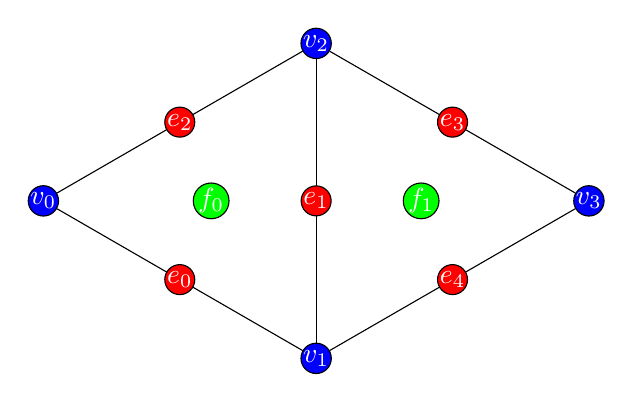
\begin{tikzpicture}[scale=2.0]
  \tikzstyle{vertex}  = [text=blue]
  \tikzstyle{vertexV} = [circle,inner sep=0pt,draw=black,fill=blue,text=white]
  \tikzstyle{edge}    = [text=red]
  \tikzstyle{edgeV}   = [circle,inner sep=0pt,draw=black,fill=red,text=white]
  \tikzstyle{face}    = [text=green]
  \tikzstyle{faceV}   = [circle,inner sep=0pt,draw=black,fill=green,text=white]
  \tikzstyle{sec}     = [->]
  % Doublet mesh with values for P_3
  \path (-1.732, 0.0) node[vertexV](dv0) {$v_0$};
  \path ( 0.0,  -1.0) node[vertexV](dv1) {$v_1$};
  \path ( 0.0,   1.0) node[vertexV](dv2) {$v_2$};
  \path ( 1.732, 0.0) node[vertexV](dv3) {$v_3$};
  \draw (dv0) -- (dv1) node[edgeV,pos=0.5] {$e_0$};
  \draw (dv1) -- (dv2) node[edgeV,pos=0.5] {$e_1$};
  \draw (dv2) -- (dv0) node[edgeV,pos=0.5] {$e_2$};
  \draw (dv2) -- (dv3) node[edgeV,pos=0.5] {$e_3$};
  \draw (dv3) -- (dv1) node[edgeV,pos=0.5] {$e_4$};
  \path (-0.6667, 0.0) node[faceV](f0) {$f_0$};
  \path ( 0.6667, 0.0) node[faceV](f1) {$f_1$};
\end{tikzpicture}
\caption{A 2D doublet mesh, two triangles sharing an edge.}
\label{fig:doubletMesh}
\end{figure}
which can also be represented as the DAG
\begin{figure}
\centering
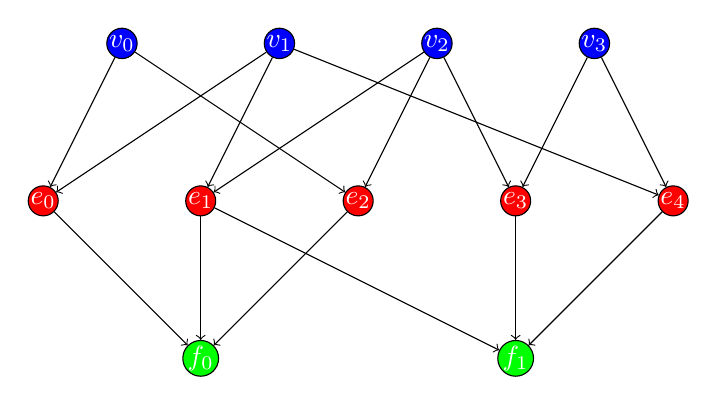
\begin{tikzpicture}[scale=2.0]
  \tikzstyle{vertex}  = [text=blue]
  \tikzstyle{vertexV} = [circle,inner sep=0pt,draw=black,fill=blue,text=white]
  \tikzstyle{edge}    = [text=red]
  \tikzstyle{edgeV}   = [circle,inner sep=0pt,draw=black,fill=red,text=white]
  \tikzstyle{face}    = [text=green]
  \tikzstyle{faceV}   = [circle,inner sep=0pt,draw=black,fill=green,text=white]
  \tikzstyle{sec}     = [->]
  % DAG for doublet
  \path (-1.5, 2.0) node[vertexV](dv0) {$v_0$};
  \path (-0.5, 2.0) node[vertexV](dv1) {$v_1$};
  \path ( 0.5, 2.0) node[vertexV](dv2) {$v_2$};
  \path ( 1.5, 2.0) node[vertexV](dv3) {$v_3$};
  \draw (-2.0, 1.0) node[edgeV](e0) {$e_0$};
  \draw (-1.0, 1.0) node[edgeV](e1) {$e_1$};
  \draw ( 0.0, 1.0) node[edgeV](e2) {$e_2$};
  \draw ( 1.0, 1.0) node[edgeV](e3) {$e_3$};
  \draw ( 2.0, 1.0) node[edgeV](e4) {$e_4$};
  \path (-1.0, 0.0) node[faceV](f0) {$f_0$};
  \path ( 1.0, 0.0) node[faceV](f1) {$f_1$};
  \draw[sec] (dv0) -- (e0);
  \draw[sec] (dv1) -- (e0);
  \draw[sec] (dv1) -- (e1);
  \draw[sec] (dv2) -- (e1);
  \draw[sec] (dv2) -- (e2);
  \draw[sec] (dv0) -- (e2);
  \draw[sec] (dv2) -- (e3);
  \draw[sec] (dv3) -- (e3);
  \draw[sec] (dv3) -- (e4);
  \draw[sec] (dv1) -- (e4);
  \draw[sec] (e0)  -- (f0);
  \draw[sec] (e1)  -- (f0);
  \draw[sec] (e2)  -- (f0);
  \draw[sec] (e1)  -- (f1);
  \draw[sec] (e3)  -- (f1);
  \draw[sec] (e4)  -- (f1);
\end{tikzpicture}
\caption{The Hasse diagram for our 2D doublet mesh, expressed as a DAG.}
\label{fig:doubletSieve}
\end{figure}
To use the PETSc API, we first consecutively number the mesh pieces. The PETSc convention is to number first cells,
then vertices, then faces, and then edges, but the user is free to violate this convention. First, we declare the set of
points present in a mesh,
\begin{lstlisting}
DMPlexSetChart(dm, 0, 11);
\end{lstlisting}
We then define the covering relation, which we call the \textit{cone}, which are also the in-edges in the DAG. In order
to preallocate correctly, we first setup sizes,
\begin{lstlisting}
DMPlexSetConeSize(dm, 0, 3);
DMPlexSetConeSize(dm, 1, 3);
DMPlexSetConeSize(dm, 6, 2);
DMPlexSetConeSize(dm, 7, 2);
DMPlexSetConeSize(dm, 8, 2);
DMPlexSetConeSize(dm, 9, 2);
DMPlexSetConeSize(dm, 10, 2);
DMSetUp(dm);
\end{lstlisting}
and then point values,
\begin{lstlisting}
DMPlexSetCone(dm, 0, [6, 7, 8]);
DMPlexSetCone(dm, 1, [7, 9, 10]);
DMPlexSetCone(dm, 6, [2, 3]);
DMPlexSetCone(dm, 7, [3, 4]);
DMPlexSetCone(dm, 8, [4, 2]);
DMPlexSetCone(dm, 9, [4, 5]);
DMPlexSetCone(dm, 10, [5, 3]);
\end{lstlisting}

There is also an API for the dual relation, using \lstinline{DMPlexSetSupportSize()} and \break\lstinline{DMPlexSetSupport()}, but this can be
calculated automatically by calling
\begin{lstlisting}
DMPlexSymmetrize(dm);
\end{lstlisting}
In order to support efficient queries, we also want to construct fast search structures, indices, for the different
types of points, which is done using
\begin{lstlisting}
DMPlexStratify(dm);
\end{lstlisting}

\section{Data on Unstructured Grids} \sindex{PetscSection}

The strongest links between solvers and discretizations are,
\begin{itemize}
  \item the layout of data over the mesh,
  \item problem partitioning, and
  \item ordering of unknowns.
\end{itemize}
To enable modularity, we encode the operations above in simple data structures that can be understood by the linear
algebra engine in PETSc without any reference to the mesh (topology) or discretization (analysis).

\subsection{Data Layout}

Data is associated to a mesh using the \lstinline{PetscSection} object. A \lstinline{PetscSection} can be thought of as a generalization of
\lstinline{PetscLayout}, in the same way that a fiber bundle is a generalization of the normal Euclidean basis used in linear
algebra. With \lstinline{PetscLayout}, we associate a unit vector ($e_i$) with every point in the space, and just divide up points
between processes. Using \lstinline{PetscSection}, we can associate a set of dofs, a small space $\{e_k\}$, with every point, and
though our points must be contiguous like \lstinline{PetscLayout}, they can be in any range $[\mathrm{pStart}, \mathrm{pEnd})$.

The sequence for setting up any \lstinline{PetscSection} is the following:
\begin{enumerate}
  \item Specify the chart,
  \item Specify the number of dofs per point, and
  \item Set up the \lstinline{PetscSection}.
\end{enumerate}
For example, using the mesh from Fig.~\ref{fig:doubletMesh}, we can layout data for a continuous Galerkin $P_3$ finite
element method,
\begin{lstlisting}
PetscInt pStart, pEnd, cStart, cEnd, c, vStart, vEnd, v, eStart, eEnd, e;

DMPlexGetChart(dm,  &pStart,  &pEnd);
DMPlexGetHeightStratum(dm, 0,  &cStart,  &cEnd);
DMPlexGetHeightStratum(dm, 1,  &eStart,  &eEnd);
DMPlexGetDepthStratum(dm, 0,  &vStart, &vEnd);
PetscSectionSetChart(s, pStart, pEnd);
for(c = cStart; c < cEnd; ++c)
    PetscSectionSetDof(s, c, 1);
for(v = vStart; v < vEnd; ++v)
    PetscSectionSetDof(s, v, 1);
for(e = eStart; e < eEnd; ++e)
    PetscSectionSetDof(s, e, 2);
PetscSectionSetUp(s);
\end{lstlisting}
Now a PETSc local vector can be created manually using this layout,
\begin{lstlisting}
PetscSectionGetStorageSize(s, &n);
VecSetSizes(localVec, n, PETSC_DETERMINE);
VecSetFromOptions(localVec);
\end{lstlisting}
however it is usually easier to use the \lstinline{DM} directly, which also provides global vectors,
\begin{lstlisting}
DMSetDefaultSection(dm, s);
DMGetLocalVector(dm, &localVec);
DMGetGlobalVector(dm, &globalVec);
\end{lstlisting}

\subsection{Partitioning and Ordering}

In exactly the same way as \lstinline{MatPartitioning} and \lstinline{MatOrdering}, we encode the results of a partition or order in an
IS. However, the graph we are dealing with now is not the adjacency graph of the problem Jacobian, but the mesh
itself. Once the mesh is partitioned and reordered, we used the data layout from a \lstinline{PetscSection} to automatically derive
a problem partitioning/ordering.

\section{Evaluating Residuals} \sindex{Residual Evaluation}

The evaluation of a residual, or Jacobian, for most discretizations has the following general form:
\begin{itemize}
  \item Traverse the mesh, picking out pieces which in general overlap,

  \item Extract some values from the solution vector, associated with this piece,

  \item Calculate some values for the piece, and

  \item Insert these values into the residual vector
\end{itemize}
\lstinline{DMPlex} separates these different concerns by passing sets of points, which are just integers, from mesh traversal
routines to data extraction routines and back. In this way, the \lstinline{PetscSection} which structures the data inside a \lstinline{Vec} does
not need to know anything about the mesh inside a \lstinline{DMPlex}.

The most common mesh traversal is the transitive closure of a point, which is exactly the transitive closure of a point
in the DAG using the covering relation. Note that this closure can be calculated orienting the arrows in either
direction. For example, in a finite element calculation, we calculate an integral over the closure of each element, and
then sum up the contributions to the basis function coefficients. The closure of the element can be expressed discretely
as the transitive closure of the element point in the mesh DAG, where each point also has an orientation. Then we can
retrieve the data using \lstinline{PetscSection} methods,
\begin{lstlisting}
PetscScalar *a;
PetscInt     numPoints, *points = NULL, p;

VecGetArray(u,&a);
DMPlexGetTransitiveClosure(dm,cell,PETSC_TRUE,&numPoints,&points);
for (p = 0; p <= numPoints*2; p += 2) {
  PetscInt dof, off, d;

  PetscSectionGetDof(section, points[p], &dof);
  PetscSectionGetOffset(section, points[p], &off);
  for=(d = 0; d <= dof; ++d) {
    myfunc(a[off+d]);
  }
}
DMPlexRestoreTransitiveClosure(dm, cell, PETSC_TRUE, &numPoints, &points);
VecRestoreArray(u, &a);
\end{lstlisting}
This operation is so common, that we have built a convenience method around it which returns the values in a contiguous
array, correctly taking into account the orientations of various mesh points,
\begin{lstlisting}
const PetscScalar *values;
PetscInt           csize;

DMPlexVecGetClosure(dm, section, u, cell, &csize, &values);
/* Do integral in quadrature loop */
DMPlexVecRestoreClosure(dm, section, u, cell, &csize, &values);
DMPlexVecSetClosure(dm, section, residual, cell, &r, ADD_VALUES);
\end{lstlisting}
A simple example of this kind of calculation is in \lstinline{DMPlexComputeL2Diff()}. Note that there is no restriction on the
type of cell or dimension of the mesh in the code above, so it will work for polyhedral cells, hybrid meshes, and meshes
of any dimension, without change. We can also reverse the covering relation, so that the code works for finite volume
methods where we want the data from neighboring cells for each face
\begin{lstlisting}
PetscScalar *a;
PetscInt     points[2*2], numPoints, p, dofA, offA, dofB, offB;

VecGetArray(u,  &a);
DMPlexGetTransitiveClosure(dm, cell, PETSC_FALSE, &numPoints, &points);
assert(numPoints == 2);
PetscSectionGetDof(section, points[0*2], &dofA);
PetscSectionGetDof(section, points[1*2], &dofB);
assert(dofA == dofB);
PetscSectionGetOffset(section, points[0*2], &offA);
PetscSectionGetOffset(section, points[1*2], &offB);
myfunc(a[offA], a[offB]);
VecRestoreArray(u, &a);
\end{lstlisting}
This kind of calculation is used in \lstinline{TS} \href{http://www.mcs.anl.gov/petsc/petsc-current/src/ts/examples/tutorials/ex11.c.html}{\trl{$PETSC_DIR/src/ts/examples/tutorials/ex11.c}}.

\section{Networks}
Built on top of \lstinline{DMPlex}, the \lstinline{DMNetwork} subclass provides abstractions for representing general unstructured
networks such as communication networks, power grid, computer networks, transportation networks, electrical circuits, graphs, and others.

\subsection{Application flow}
The general flow of an application code using \lstinline{DMNetwork} is as follows:

\begin{enumerate}
  \item Create a network object and a ``component'' library:
\begin{lstlisting}
DMNetworkCreate(MPI_Comm, DM*);
\end{lstlisting}
  creates an empty network object. A ``component'' is specific application data at a node/edge of the network required for its residual evaluation. For example, components could be resistor, inductor data for circuit applications, edge weights for graph problems, generator/transmission line data for power grids. Components are registered by calling
\begin{lstlisting}
DMNetworkRegisterComponent(DM,const char* name, PetscInt size, PetscInt* compkey);
\end{lstlisting}
  Here, \lstinline{name} is the component name,\lstinline{size} is the size of component data type, and \lstinline{compkey} is an integer key that can be used for
  setting/getting the component at a node or an edge.
  \item Set network size (number of nodes, edges), edge connectivity.
  \item Set the bare layout (graph) of the network
\begin{lstlisting}
DMNetworkLayoutSetUp(DM dm);
\end{lstlisting}
\begin{lstlisting}
DMNetworkSetSizes(DM dm, PetscInt nnodes, PetscInt nedges, PetscInt Nnodes, PetscInt Nedges);
\end{lstlisting}
\begin{lstlisting}
DMNetworkSetEdgeList(DM dm, int edgeconns[]);
\end{lstlisting}
  \item Set components and number of variables for nodes/edges.
\begin{lstlisting}
DMNetworkAddComponent(DM dm, PetscInt p,PetscInt component,void* component);
\end{lstlisting}
  Multiple components can be added at a node/edge.
\begin{lstlisting}
DMNetworkSetNumVariables(DM dm,PetscInt p,PetscInt nvar);
\end{lstlisting}
\begin{lstlisting}
DMNetworkAddNumVariables(DM dm,PetscInt p,PetscInt nvar);
\end{lstlisting}
  \item Signal network ready to be distributed.
\begin{lstlisting}
DMSetUp(DM dm);
\end{lstlisting}
  \item Distribute the network (also moves components attached with nodes/edges)
\begin{lstlisting}
DMNetworkDistribute(DM oldDM, const char partitioner[], PetscInt overlap,DM *distDM);
\end{lstlisting}
\item Hook up the \lstinline{DM} with the solver: \lstinline{KSPSetDM()}, \lstinline{SNESSetDM()}, \lstinline{TSSetDM()}
\end{enumerate}

\subsection{Utility functions}
  \lstinline{DMNetwork} provides functions for obtaining iterators for nodes/edges, checking the ``ghost''
  status of a node (vertex), and retrieving local/global indices of node/edge variables for inserting
  elements in vectors/matrices.
\begin{lstlisting}
DMNetworkGetEdgeRange(DM dm,PetscInt *eStart,PetscInt *eEnd);
\end{lstlisting}
\begin{lstlisting}
DMNetworkGetVertexRange(DM dm,PetscInt *vStart, PetscInt *vEnd);
\end{lstlisting}
\begin{lstlisting}
DMNetworkIsGhostVertex(DM dm,PetscInt p,PetscBool *isghost);
\end{lstlisting}
\begin{lstlisting}
DMNetworkGetVariableOffset(DM dm,PetscInt p,PetscInt *offset);
\end{lstlisting}
\begin{lstlisting}
DMNetworkGetVariableGlobalOffset(DM dm,PetscInt p,PetscInt *offsetg);
\end{lstlisting}
In network applications, one frequently needs to find the supporting edges for a node or
the connecting nodes covering an edge. These can be obtained by the following two routines.
\begin{lstlisting}
DMNetworkGetConnectedNodes(DM dm,PetscInt edge,const PetscInt *vertices[]);
\end{lstlisting}
\begin{lstlisting}
DMNetworkGetSupportingEdges(DM dm,PetscInt vertex,PetscInt *nedges,const PetscInt *edges[]) ;
\end{lstlisting}

\subsection{Retrieving components}
The components set at nodes/edges are stored in a container that can be accessed by
\begin{lstlisting}
DMNetworkGetComponentDataArray(DM dm,DMNetworkComponentGenericDataType **componentdataarray);
\end{lstlisting}
  Using \lstinline{componentdataarray}, individual components set at a node/edge can be retrieved by
\begin{lstlisting}
DMNetworkGetComponentTypeOffset(DM dm,PetscInt p, PetscInt compnum, PetscInt *compkey, PetscInt *offset);
\end{lstlisting}
\lstinline{compkey} is the key set by \lstinline{DMNetworkRegisterComponent}. An example of accessing and retrieving the components at nodes is:

\begin{lstlisting}
DMNetworkComponentGenericDataType *arr; 
PetscInt Start, End, numcomps,offset,key,v,compnum; 

DMNetworkGetComponentDataArray(dm,  &arr); 
DMNetworkGetVertexRange(dm, &Start, &End); 
for(v=Start; v  < End; v++) { 
  DMNetworkGetNumComponents(dm,v, &numcomps); 
  for(compnum=0; compnum < numcomps;compnum++) {
    DMNetworkGetComponentTypeOffset(dm,v,compnum, &key, &offset); 
    compdata = (UserCompDataType)(arr+offset); 
  }
}
\end{lstlisting}

% --------------------------------------------------------------------
%                            PART 3
% --------------------------------------------------------------------
\cleardoublepage
\part{Additional Information}
\label{part_usefulstuff}

%------------------------------------------------------------------
\cleardoublepage
\chapter{PETSc for Fortran Users}
\label{ch_fortran}

Most of the functionality of PETSc can be obtained by people who
program purely in Fortran 77 or Fortran 90.
The PETSc Fortran interface works with both F77 and F90 compilers.

Since Fortran77 does not provide type checking of routine input/output
parameters, we find that many errors encountered within PETSc Fortran
programs result from accidentally using incorrect calling sequences.
Such mistakes are immediately detected during compilation when using
C/C++.  Thus, using a mixture of C/C++ and Fortran often works well
for programmers who wish to employ Fortran for the core numerical
routines within their applications.  In particular, one can
effectively write PETSc driver routines in C/C++, thereby preserving
flexibility within the program, and still use Fortran when desired for
underlying numerical computations. With Fortran 90 compilers we now
can provide some type checking from Fortran.

\section{C vs. Fortran Interfaces}

Only a few differences exist between the C and Fortran PETSc
interfaces, all of which are due to Fortran 77 syntax limitations.
Since PETSc is primarily written in C, the FORTRAN 90
dynamic allocation is not easily accessible.
All Fortran routines have the same names as the corresponding C
versions, and PETSc command line options are fully supported. The
routine arguments follow the usual Fortran conventions; the user need
not worry about passing pointers or values.  The calling sequences
for the Fortran version are in most cases identical to the C version,
except for the error checking variable discussed in
Section \ref{sec_fortran_errors} and a few routines listed in
Section \ref{sec_fortran_exceptions}.

\subsection{Include Files}
\label{sec_fortran_includes}

The Fortran include files for PETSc are located in the directory
\trl{${PETSC_DIR}/include/petsc/finclude} and should be used via statements
such as the following:
\begin{lstlisting}
#include "petsc/finclude/includefile.h"
\end{lstlisting}
Since one must be very careful to include each file no more than once
in a Fortran routine, application programmers must manually include
each file needed for the various PETSc libraries within their
program.  This approach differs from the PETSc C/C++ interface, where
the user need only include the highest level file, for example, \trl{
petscsnes.h}, which then automatically includes all of the required lower
level files.  As shown in the examples of Section
\ref{sec_fortran-examples}, in Fortran one must explicitly list {\em
each} of the include files. One must employ
the Fortran file suffix \trl{.F}
rather than \trl{.f}.  This convention enables use of the CPP
preprocessor, which allows the use of the \lstinline{#include} statements
that define PETSc objects and variables. (Familiarity with the CPP
preprocessor is not needed for writing PETSc Fortran code; one can simply
begin by copying a PETSc Fortran example and its corresponding
makefile.)

For some of the Fortran 90 functionality of PETSc and type checking
of PETSc function calls you can use
\begin{lstlisting}
#include "petsc/finclude/includefile.h"
#include "petsc/finclude/includefile.h90"
\end{lstlisting}
See the manual page UsingFortran for how you can use PETSc Fortran
module files in your code.

\subsection{Error Checking}
\label{sec_fortran_errors}

In the Fortran version, each PETSc routine has as its final argument
an integer error variable, in contrast to the C convention of
providing the error variable as the routine's return value.  The error
code is set to be nonzero if an error has been detected; otherwise, it
is zero.  For example, the Fortran and C variants of \lstinline{KSPSolve()} are
given, respectively, below, where \lstinline{ierr} denotes the error variable:
\begin{lstlisting}
call KSPSolve(KSP ksp,Vec b,Vec x,PetscErrorCode ierr) ! Fortran
ierr = KSPSolve(KSP ksp,Vec b,Vec x);                  /* C */
\end{lstlisting}

Fortran programmers
can check these error codes with
\lstinline{CHKERRQ(ierr)}, which terminates all processes when an error is
encountered.  Likewise, one can set error codes within Fortran programs by
using \lstinline{SETERRQ(comm,p,' ',ierr)}, which again terminates all processes
upon detection of an error.
Note that complete error tracebacks with
\lstinline{CHKERRQ()} and \lstinline{SETERRQ()}, as described in Section
\ref{sec_simple} for C routines, are {\em not} directly supported for
Fortran routines; however, Fortran programmers can easily use the
error codes in writing their own tracebacks.  For example, one could
use code such as the following:
\begin{lstlisting}
call KSPSolve(ksp,b,x,ierr)
if (ierr .ne. 0) then
   print*, 'Error in routine ...'
   return
end if
\end{lstlisting}

The most common reason for crashing PETSc Fortran code is forgetting the
final \lstinline{ierr} argument.

\subsection{Array Arguments}
\label{sec_fortranarrays}

Since Fortran 77 does not allow arrays to be returned in routine
arguments, all PETSc routines that return arrays, such as
\lstinline{VecGetArray()}, \lstinline{MatDenseGetArray()},
and \lstinline{ISGetIndices()},
are defined slightly differently in Fortran than in C.
Instead of returning the array itself, these routines
accept as input a user-specified array of dimension one and return an
integer index to the actual array used for data storage within PETSc.
The Fortran interface for several routines is as follows:
\begin{lstlisting}
double precision xx_v(1), aa_v(1)
PetscErrorCode ierr
integer          ss_v(1), dd_v(1), nloc
PetscOffset      ss_i, xx_i, aa_i, dd_i
Vec x
Mat A
IS  s
DM  d 

call VecGetArray(x,xx_v,xx_i,ierr)
call MatDenseGetArray(A,aa_v,aa_i,ierr)
call ISGetIndices(s,ss_v,ss_i,ierr)
\end{lstlisting}

To access array elements directly, both the user-specified array and
the integer index {\em must} then be used together.
For example, the following Fortran program fragment illustrates
directly setting the values of a vector array instead of using \lstinline{VecSetValues()}.  Note the (optional) use of the preprocessor
\lstinline{#define} statement to enable array manipulations in the conventional
Fortran manner.
\begin{lstlisting}
#define xx_a(ib)  xx_v(xx_i + (ib))

   double precision xx_v(1)
   PetscOffset      xx_i
   PetscErrorCode ierr
   integer          i, n
   Vec              x
   call VecGetArray(x,xx_v,xx_i,ierr)
   call VecGetLocalSize(x,n,ierr)
   do 10, i=1,n
     xx_a(i) = 3*i + 1
10 continue
   call VecRestoreArray(x,xx_v,xx_i,ierr)
\end{lstlisting}
Figure \ref{fig_vec2-Fortran} contains an example of using \lstinline{VecGetArray()}
within a Fortran routine.

Since in this case the array is accessed directly from Fortran,
indexing begins with 1, not 0 (unless the array is declared as \lstinline{xx_v(0:1)}).
This is different from the use of \lstinline{VecSetValues()}
where, indexing always starts with 0.

{\em Note}: If using \lstinline{VecGetArray()}, \lstinline{MatDenseGetArray()}, or \lstinline{ISGetIndices()},
from Fortran, the user {\em must not} compile the Fortran code with options
to check for ``array entries out of bounds'' (e.g., on the IBM RS/6000 this
is done with the \trl{-C} compiler option, so never use the \trl{-C} option with this).

\subsection{Calling Fortran Routines from C (and C Routines from Fortran)}


Different machines have
different methods of naming Fortran routines called from C
(or C routines called from Fortran). Most Fortran compilers change
all the capital letters in Fortran routines to lowercase. On some machines, the
Fortran compiler appends an underscore to the end of each Fortran
routine name; for example, the Fortran routine \lstinline{Dabsc()}
would be called from C with \lstinline{dabsc_()}.  Other machines
change all the letters in Fortran routine names to capitals.

PETSc provides two macros (defined in C/C++) to help write
portable code that mixes C/C++ and Fortran. They are
\lstinline{PETSC_HAVE_FORTRAN_UNDERSCORE} and \lstinline{PETSC_HAVE_FORTRAN_CAPS}
\findex{PETSC_HAVE_FORTRAN_UNDERSCORE} \findex{PETSC_HAVE_FORTRAN_CAPS},
which are defined in the file \trl{${PETSC_DIR}/${PETSC_ARCH}/include/petscconf.h}.
The macros are used, for example, as follows:
\begin{lstlisting}
#if defined(PETSC_HAVE_FORTRAN_CAPS)
#define dabsc_ DMDABSC
#elif !defined(PETSC_HAVE_FORTRAN_UNDERSCORE)
#define dabsc_ dabsc
#endif
.....
dabsc_( &n,x,y); /* call the Fortran function */
\end{lstlisting}


\subsection{Passing Null Pointers}

In several PETSc C functions, one has the option of passing a 0 (null)
argument (for example, the fifth argument of \lstinline{MatCreateSeqAIJ()}).
From Fortran, users {\em must} pass \lstinline{PETSC_NULL_XXX} to indicate a
null argument (where \lstinline{XXX} is \lstinline{INTEGER}, \lstinline{DOUBLE}, \lstinline{CHARACTER},
or \lstinline{SCALAR} depending on the type of argument required);
\findex{PETSC_NULL_INTEGER} passing \findex{PETSC_NULL_SCALAR} 0 from
\findex{PETSC_NULL_DOUBLE} Fortran \findex{PETSC_NULL_CHARACTER}  will crash
the code.   Note
that the C convention of passing NULL (or 0) {\em cannot}
be used.  For example, when no options prefix is desired in the
routine \lstinline{PetscOptionsGetInt()}, one must use the following command in
Fortran:
\begin{lstlisting}
call PetscOptionsGetInt(PETSC_NULL_OBJECT,PETSC_NULL_OBJECT,PETSC_NULL_CHARACTER,'-name',N,flg,ierr)
\end{lstlisting}

This Fortran requirement is inconsistent with C, where the
user can employ \lstinline{NULL} for all null arguments.

\subsection{Duplicating Multiple Vectors}
\label{sec_fortvecd}

The Fortran interface to \lstinline{VecDuplicateVecs()} differs slightly
from the C/C++ variant because Fortran does not allow arrays to be
returned in routine arguments.  To create \lstinline{n} vectors of the same
format as an existing vector, the user must declare a vector array,
\lstinline{v_new} of size \lstinline{n}.  Then, after \lstinline{VecDuplicateVecs()} has
been called, \lstinline{v_new} will contain (pointers to) the new PETSc
vector objects.  When finished with the vectors, the user should
destroy them by calling \lstinline{VecDestroyVecs()}.
For example, the following code fragment
duplicates \lstinline{v_old} to form two new vectors, \lstinline{v_new(1)} and \lstinline{v_new(2)}.
\begin{lstlisting}
Vec     v_old, v_new(2)
integer ierr
PetscScalar  alpha
....
call VecDuplicateVecs(v_old,2,v_new,ierr)
alpha = 4.3
call VecSet(v_new(1),alpha,ierr)
alpha = 6.0
call VecSet(v_new(2),alpha,ierr)
....
call VecDestroyVecs(2, &v_new,ierr)
\end{lstlisting}

\subsection{Matrix, Vector and IS Indices}

All matrices, vectors and \lstinline{IS} in PETSc use zero-based indexing, regardless
of whether C or Fortran is being used.  The interface routines, such
as \lstinline{MatSetValues()} and \lstinline{VecSetValues()}, always use zero
indexing.  See Section \ref{sec_matoptions} for further details.

\subsection{Setting Routines}

When a function pointer is passed as an argument to a PETSc function, such as
the test in \lstinline{KSPSetConvergenceTest()}, it is assumed that this pointer references
a routine written in the same language as the PETSc interface function that was
called. For instance, if \lstinline{KSPSetConvergenceTest()} is called from C, the test
argument is assumed to be a C function. Likewise, if it is called from Fortran,
the test is assumed to be written in Fortran.

\subsection{Compiling and Linking Fortran Programs}
\label{sec_fortcompile}

Figure \ref{fig_make1} shows a sample makefile that can be used for
PETSc programs.  In this makefile, one can compile and run a debugging version
of the Fortran program \trl{ex3.F} with the actions \trl{make}  \trl{ex3} and
\trl{make} \trl{runex3}, respectively. The compilation command is restated below:
\begin{lstlisting}
ex3: ex3.o 
       -${FLINKER}} -o ex3 ex3.o ${PETSC_LIB}
        ${RM} ex3.o
\end{lstlisting}

\subsection{Routines with Different Fortran Interfaces}
\label{sec_fortran_exceptions}

The following Fortran routines differ slightly from their C counterparts; see the
manual pages and previous discussion in this chapter for details:
\begin{lstlisting}
PetscInitialize(char *filename,int ierr)
PetscError(MPI_COMM,int err,char *message,int ierr)
VecGetArray(), MatDenseGetArray()
ISGetIndices(), 
VecDuplicateVecs(), VecDestroyVecs()
PetscOptionsGetString()
\end{lstlisting}
The following functions are not supported in Fortran:
\begin{lstlisting}
PetscFClose(), PetscFOpen(), PetscFPrintf(), PetscPrintf()
PetscPopErrorHandler(), PetscPushErrorHandler()
PetscInfo()
PetscSetDebugger()
VecGetArrays(), VecRestoreArrays()
PetscViewerASCIIGetPointer(), PetscViewerBinaryGetDescriptor()
PetscViewerStringOpen(), PetscViewerStringSPrintf()
PetscOptionsGetStringArray()
\end{lstlisting}

\subsection{Fortran90}

PETSc includes limited support for direct use of Fortran90 pointers.
Current routines include:
\begin{lstlisting}
VecGetArrayF90(), VecRestoreArrayF90()
VecGetArrayReadF90(), VecRestoreArrayReadF90()
VecDuplicateVecsF90(), VecDestroyVecsF90()
DMDAVecGetArrayF90(), DMDAVecGetArrayReadF90(), ISLocalToGlobalMappingGetIndicesF90()
MatDenseGetArrayF90(), MatDenseRestoreArrayF90()
ISGetIndicesF90(), ISRestoreIndicesF90()
\end{lstlisting}
See the manual pages for details and pointers to example programs.  To
use the routines \lstinline{VecGetArrayF90()}, \lstinline{VecRestoreArrayF90()}, \lstinline{VecGetArrayReadF90()}, \lstinline{VecRestoreArrayReadF90()},
\lstinline{VecDuplicateVecsF90()}, and \lstinline{VecDestroyVecsF90()}, one must
use the Fortran90 vector include file,
\begin{lstlisting}
#include "petsc/finclude/petscvec.h90"
\end{lstlisting}
Analogous include files for other libraries are \trl{petscdm.h90},
\trl{petscmat.h90}, and \trl{petscis.h90}.

\section{Sample Fortran77 Programs}
\label{sec_fortran-examples}

Sample programs that illustrate the PETSc interface for Fortran
are given in Figures \ref{fig_vec-Fortran} {\em --} \ref{fig_SNES-Fortran},
corresponding to
\href{http://www.mcs.anl.gov/petsc/petsc-current/src/vec/vec/examples/tests/ex19f.F.html}{\trl{${PETSC_DIR}/src/vec/vec/examples/tests/ex19f.F}},
\href{http://www.mcs.anl.gov/petsc/petsc-current/src/vec/vec/examples/tutorials/ex4f.F.html}{\trl{${PETSC_DIR}/src/vec/vec/examples/tutorials/ex4f.F}},
\break 
\href{http://www.mcs.anl.gov/petsc/petsc-current/src/sys/classes/draw/examples/tests/ex5f.F.html}{\trl{${PETSC_DIR}/src/sys/classes/draw/examples/tests/ex5f.F}}, and
\href{http://www.mcs.anl.gov/petsc/petsc-current/src/snes/examples/tutorials/ex1f.F.html}{\trl{${PETSC_DIR}/src/snes/examples/ex1f.F}}, respectively.  We also
refer Fortran programmers to the C examples listed throughout the manual,
since PETSc usage within the two languages differs only slightly.

\begin{figure}[H]
  \input{listing_vecex19ftmp.tex}
\caption{Sample Fortran Program:  Using PETSc Vectors}
\label{fig_vec-Fortran}
\end{figure}

\begin{figure}[H]
  \input{listing_vecex4ftmp.tex}
\caption{Sample Fortran Program: Setting Vector Entries and Accessing A Raw Vector Array} 
\label{fig_vec2-Fortran}
\end{figure}

\begin{figure}[H]
  \input{listing_drawex5ftmp.tex}
\caption{Sample Fortran Program:  Using PETSc PetscDraw Routines}
\label{fig_draw-Fortran}
\end{figure}

\begin{figure}[H]
  \input{listing_snesex1ftmp.tex}
\caption{Sample Fortran Program:  Using PETSc Nonlinear Solvers}
\label{fig_SNES-Fortran}
\end{figure}

%------------------------------------------------------------------
\cleardoublepage
\chapter{Using MATLAB with PETSc}
\label{ch_matlab}\sindex{MATLAB}

There are three basic ways to use MATLAB with PETSc: 
\begin{enumerate}
  \item (Section \ref{sec_matlabdump}) dumping files to be read into MATLAB,
  \item (Section \ref{sec_matlabsocket}) automatically sending data from a running PETSc program
to a MATLAB process where you may interactively type MATLAB commands (or run
scripts), and 
\item (Section \ref{sec_matlabengine}) automatically sending data back and forth between PETSc and
MATLAB where MATLAB commands are issued not interactively but from a script or
the PETSc program (this uses the MATLAB Engine).
\end{enumerate}

\section{Dumping Data for MATLAB}
\label{sec_matlabdump}
One can dump PETSc matrices and vectors to the screen (and thus save in a file via
\trl{> filename.m}) in an ASCII format that MATLAB can read in directly. This is done with the
command line options \trl{-vec_view ::ascii_matlab} or \trl{-mat_view ::ascii_matlab}. This causes the PETSc program
to print the vectors and matrices every time \lstinline{VecAssemblyEnd()} or \lstinline{MatAssemblyEnd()} are called. \findex{-vec_view ::ascii_matlab} \findex{-mat_view ::ascii_matlab} 
To provide finer control
over when and what vectors and matrices are dumped one can use the \lstinline{VecView()} and
\lstinline{MatView()} functions with a viewer type of ASCII (see \lstinline{PetscViewerASCIIOpen()},
\lstinline{PETSC_VIEWER_STDOUT_WORLD}, \lstinline{PETSC_VIEWER_STDOUT_SELF}, or \lstinline{PETSC_VIEWER_STDOUT_(MPI_Comm)}). Before calling
the viewer set the output type with, for example,
\begin{lstlisting}
PetscViewerPushFormat(PETSC_VIEWER_STDOUT_WORLD,PETSC_VIEWER_ASCII_MATLAB);
VecView(A,PETSC_VIEWER_STDOUT_WORLD);
PetscViewerPopFormat(PETSC_VIEWER_STDOUT_WORLD);  
\end{lstlisting}
The name of each PETSc variable printed for MATLAB may be set with
\begin{lstlisting}
PetscObjectSetName((PetscObject)A,"name");
\end{lstlisting}\sindex{PetscObjectSetName()}
If no name is specified, the object is given a default name using \lstinline{PetscObjectName()}.

One can also read PETSc binary files directly into MATLAB via the scripts available in \lstinline{$PETSC_DIR/share/matlab}.
This requires less disk space.

\section{Sending Data to Interactive Running MATLAB Session}
\label{sec_matlabsocket}

One creates a viewer to MATLAB via
\begin{lstlisting}
PetscViewerSocketOpen(MPI_Comm,char *machine,int port,PetscViewer *v);
\end{lstlisting}
(port is usually set to \lstinline{PETSC_DEFAULT}; use \lstinline{NULL} for the machine if the
MATLAB interactive session is running on the same machine as the PETSc program)
and then sends matrices or vectors via
\begin{lstlisting}
VecView(Vec A,v);
MatView(Mat B,v);
\end{lstlisting}
One can also send arrays or integer arrays via \lstinline{PetscIntView()}, \lstinline{PetscRealView()} and \break\lstinline{PetscScalarView()}.
One may start the MATLAB program manually or use the PETSc command
\break \lstinline{PetscStartMATLAB(MPI_Comm,char *machine,char *script,FILE **fp)}; where machine and script may be \lstinline{NULL}.

To receive the objects in MATLAB you must first make sure that \trl{${PETSC_DIR}/${PETSC_ARCH}/lib/petsc/matlab}
is in your MATLAB path. Use \lstinline{p = sopen;} (or \lstinline{p = sopen(portnum)} if you provided a port number in
your call to \lstinline{PetscViewerSocketOpen()}), then \lstinline{a = PetscBinaryRead(p);} returns the object you have passed from PETSc.
\lstinline{PetscBinaryRead()} may be called any number of times. Each call should correspond on the PETSc side with
viewing a single vector or matrix. You many call \lstinline{sclose()} to close the connection from MATLAB.
It is also possible to start your PETSc program from MATLAB via \lstinline{launch()}.

\section{Using the MATLAB Compute Engine}
\label{sec_matlabengine}

One creates access to the MATLAB engine via
\begin{lstlisting}
PetscMatlabEngineCreate(MPI_Comm comm,char *machine,PetscMatlabEngine *e);
\end{lstlisting}
where \lstinline{machine} is the name of the machine hosting MATLAB (\lstinline{NULL} may be used for localhost).
One can send objects to MATLAB via
\begin{lstlisting}
PetscMatlabEnginePut(PetscMatlabEngine e,PetscObject obj);
\end{lstlisting}
One can get objects
via
\begin{lstlisting}
PetscMatlabEngineGet(PetscMatlabEngine e,PetscObject obj);.
\end{lstlisting}
Similarly one can send arrays via
\begin{lstlisting}
PetscMatlabEnginePutArray(PetscMatlabEngine e,int m,int n,PetscScalar *array,char *name);
\end{lstlisting}
and get them back via
\begin{lstlisting}
PetscMatlabEngineGetArray(PetscMatlabEngine e,int m,int n,PetscScalar *array,char *name);
\end{lstlisting}
One cannot use MATLAB
interactively in this mode but you can send MATLAB commands via
\begin{lstlisting}
PetscMatlabEngineEvaluate(PetscMatlabEngine,"format",...);
\end{lstlisting}
where \lstinline{format} has the usual \lstinline{printf()} format.
For example,
\begin{lstlisting}
PetscMatlabEngineEvaluate(PetscMatlabEngine,"x = \%g *y + z;",avalue);
\end{lstlisting}
The name of each PETSc variable passed to Matlab may be set with
\begin{lstlisting}
PetscObjectSetName((PetscObject)A,"name");
\end{lstlisting}

Text responses can be returned from MATLAB via
\begin{lstlisting}
PetscMatlabEngineGetOutput(PetscMatlabEngine,char **);
\end{lstlisting}
or
\begin{lstlisting}
PetscMatlabEnginedPrintOutput(PetscMatlabEngine,FILE*).
\end{lstlisting}
There is a short-cut to starting the MATLAB engine
with \lstinline{PETSC_MATLAB_ENGINE_(MPI_Comm)}.

%---------------------------------------------------------------------
\cleardoublepage
\chapter{Profiling}
\label{ch_profiling} \sindex{profiling}

PETSc includes a consistent, lightweight scheme to allow the profiling
of application programs.  The PETSc routines automatically log
performance data if certain options are specified at runtime.  The
user can also log information about application codes for a complete
picture of performance.  In addition, as described in
Section~\ref{sec_ploginfo}, PETSc provides a mechanism for printing
informative messages about computations.  Section~\ref{sec_profbasic}
introduces the various profiling options in PETSc, while the
remainder of the chapter focuses on details such as monitoring
application codes and tips for accurate profiling.

\section{Basic Profiling Information}
\label{sec_profbasic}
\sindex{profiling} \sindex{logging} \sindex{timing}

If an application code and the PETSc libraries have been configured with
\trl{--with-log=1}, the default,
then various kinds of profiling of code between calls to \lstinline{PetscInitialize()} and \lstinline{PetscFinalize()} can be
activated at runtime.  The profiling options include the following:
\findex{-log_view} \findex{-info}
\findex{-log_trace}
\begin{itemize}
\item \trl{-log_view} - Prints an ASCII version of performance data
     at program's conclusion. These statistics are comprehensive and concise
     and require little overhead; thus, \trl{-log_view} is intended as
     the primary means of monitoring the performance of PETSc codes.
\item \trl{-info [infofile]} - Prints verbose information about code to
     stdout or an optional file. This option provides details about algorithms,
     data structures, etc. Since the overhead of printing such output slows a
     code, this option should not be used when evaluating a program's performance.
\item \trl{-log_trace [logfile]} - Traces the beginning and ending of all
     PETSc events.  This option, which can be used in conjunction with
     \trl{-info}, is useful to see where a program is hanging
     without running in the debugger.
\end{itemize}
 As discussed in Section~\ref{sec_mpelogs},
additional profiling can be done with MPE.

\subsection{Interpreting {\tt -log\_summary} Output: The Basics}
\label{sec_ploginfo}

As shown in Figure~\ref{fig_exprof} (in Part I), the option
\trl{-log_view} \findex{-log_view} activates printing of profile
data to standard output at the conclusion of a program.  Profiling
data can also be printed at any time within a program by calling \lstinline{PetscLogView()}.

We print performance data for each routine, organized by PETSc
libraries, followed by any user-defined events (discussed in
Section~\ref{sec_profileuser}).  For each routine, the output data
include the maximum time and floating point operation (flop) rate over
all processes.  Information about parallel performance is also
included, as discussed in the following section.

For the purpose of PETSc floating point operation counting, we define
one {\em flop} as one operation of any of the following types:
multiplication, division, addition, or subtraction.  For example, one
\lstinline{VecAXPY()} operation, which computes $y = \alpha x + y$ for
vectors of length $N$, requires $2N$ flops (consisting of $N$
additions and $N$ multiplications).  Bear in mind that flop rates
present only a limited view of performance, since memory loads and stores are
the real performance barrier.

For simplicity, the remainder of this discussion focuses on
interpreting profile data for the \lstinline{KSP} library,
which provides the linear solvers at the heart of the
PETSc package.  Recall the hierarchical organization of the PETSc
library, as shown in Figure~\ref{fig_1}.  Each \lstinline{KSP} solver
is composed of a \lstinline{PC} (preconditioner) and a \lstinline{KSP} (Krylov
subspace) part, which are in turn built on top of the \lstinline{Mat}
(matrix) and \lstinline{Vec} (vector) modules.  Thus, operations in the
\lstinline{KSP} module are composed of lower-level operations in these
packages.  Note also that the nonlinear solvers library, \lstinline{SNES},
is built on top of the \lstinline{KSP} module, and the timestepping
library, \lstinline{TS}, is in turn built on top of \lstinline{SNES}.

We briefly discuss interpretation of the sample output in
Figure~\ref{fig_exprof}, which was generated by solving a linear
system on one process using restarted GMRES and ILU
preconditioning.  The linear solvers in \lstinline{KSP} consist of two
basic phases, \lstinline{KSPSetUp()} and \lstinline{KSPSolve()}, each of which
consists of a variety of actions, depending on the particular
solution technique.
For the case of using the \lstinline{PCILU} preconditioner and \lstinline{KSPGMRES}
Krylov subspace method, the breakdown of PETSc routines is listed below.
As indicated by the levels of indentation, the
operations in \lstinline{KSPSetUp()} include all of the operations within
\lstinline{PCSetUp()}, which in turn include \lstinline{MatILUFactor()}, and so on.
\begin{tightitemize}
  \item \lstinline{KSPSetUp} - Set up linear solver
   \begin{tightitemize}
     \item \lstinline{PCSetUp} - Set up preconditioner
    \begin{tightitemize}
      \item \lstinline{MatILUFactor} - Factor preconditioning matrix
      \begin{tightitemize}
        \item \lstinline{MatILUFactorSymbolic} - Symbolic factorization phase
        \item \lstinline{MatLUFactorNumeric} - Numeric factorization phase
      \end{tightitemize}
    \end{tightitemize}
\end{tightitemize}
 \item \lstinline{KSPSolve} - Solve linear system
   \begin{tightitemize}
     \item \lstinline{PCApply} - Apply preconditioner
    \begin{tightitemize}
      \item \lstinline{MatSolve} - Forward/backward triangular solves
    \end{tightitemize}
  \item \lstinline{KSPGMRESOrthog} - Orthogonalization in GMRES
    \begin{tightitemize}
      \item \lstinline{VecDot} or \lstinline{VecMDot} - Inner products
    \end{tightitemize}
  \item \lstinline{MatMult} - Matrix-vector product
  \item \lstinline{MatMultAdd} - Matrix-vector product + vector addition
    \begin{tightitemize}
      \item \lstinline{VecScale}, \lstinline{VecNorm}, \lstinline{VecAXPY}, \lstinline{VecCopy}, ...
    \end{tightitemize}
  \end{tightitemize}
\end{tightitemize}

The summaries printed via \trl{-log_view} reflect this
routine hierarchy. For example, the performance summaries for a
particular high-level routine such as \lstinline{KSPSolve()} include all of
the operations accumulated in the lower-level components that
make up the routine.

Admittedly, we do not currently present the output with
\trl{-log_view} so that the hierarchy of PETSc operations is completely
clear, primarily because we have not determined a clean and uniform
way to do so throughout the library.  Improvements may follow.
However, for a particular problem, the user should generally have
an idea of the basic operations that are required for its
implementation (e.g., which operations are performed when using GMRES
and ILU, as described above), so that interpreting the \trl{-log_view}
data should be relatively straightforward.

\subsection{Interpreting {\tt -log\_summary} Output: Parallel Performance}
\label{sec_parperformance}

We next discuss performance summaries for parallel programs,
\findex{-log_view} as shown within Figures~\ref{fig_exparprof}
and~\ref{fig_exparprof2}, which present the combined output generated by
the \trl{-log_view} option.  The program that generated this data is
\href{http://www.mcs.anl.gov/petsc/petsc-current/src/ksp/ksp/examples/tutorials/ex10.c.html}{\trl{${PETSC_DIR}/src/ksp/ksp/examples/ex10.c}}.  
The code loads a
matrix and right-hand-side vector from a binary file and then solves
the resulting linear system; the program then repeats this process for
a second linear system.  This particular case was run on four
processors of an IBM SP, using restarted GMRES and the block Jacobi
preconditioner, where each block was solved with ILU.

Figure~\ref{fig_exparprof} presents an overall performance summary,
including times, floating-point operations, computational rates, and
message-passing activity (such as the number and size of messages sent
and collective operations).  Summaries for various user-defined stages
of monitoring (as discussed in Section~\ref{sec_profstages}) are also
given. Information about the various phases of computation then follow
(as shown separately here in Figure~\ref{fig_exparprof2}).
Finally, a summary of memory usage and object creation and destruction
is presented.

\begin{figure}[tb]
  \begin{outputlisting}[\tiny\ttfamily] 
mpiexec -n 4 ./ex10 -f0 medium -f1 arco6 -ksp_gmres_classicalgramschmidt -log_view -mat_type baij \
            -matload_block_size 3 -pc_type bjacobi -options_left

Number of iterations =  19
Residual norm = 7.7643e-05
Number of iterations =  55
Residual norm = 6.3633e-01

---------------------------------------------- PETSc Performance Summary: ----------------------------------------------

ex10 on a rs6000 named p039 with 4 processors, by mcinnes Wed Jul 24 16:30:22 1996

                         Max         Min        Avg        Total
Time (sec):           3.289e+01      1.0   3.288e+01
Objects:              1.130e+02      1.0   1.130e+02
Flops:                2.195e+08      1.0   2.187e+08   8.749e+08
Flops/sec:            6.673e+06      1.0               2.660e+07
MPI Messages:         2.205e+02      1.4   1.928e+02   7.710e+02
MPI Message Lengths:  7.862e+06      2.5   5.098e+06   2.039e+07
MPI Reductions:       1.850e+02      1.0

Summary of Stages:  ---- Time ------  ----- Flops -------  -- Messages -- -- Message-lengths -- Reductions -
                      Avg      %Total    Avg     %Total   counts   %Total    avg      %Total   counts  %Total
 0:  Load System 0: 1.191e+00    3.6% 3.980e+06   0.5%  3.80e+01    4.9%  6.102e+04   0.3%  1.80e+01   9.7%
 1:    KSPSetup 0:  6.328e-01    2.5% 1.479e+04   0.0%  0.00e+00    0.0%  0.000e+00   0.0%  0.00e+00   0.0%
 2:    KSPSolve 0:  2.269e-01    0.9% 1.340e+06   0.0%  1.52e+02   19.7%  9.405e+03   0.0%  3.90e+01  21.1%
 3:  Load System 1: 2.680e+01  107.3% 0.000e+00   0.0%  2.10e+01    2.7%  1.799e+07  88.2%  1.60e+01   8.6%
 4:    KSPSetup 1:  1.867e-01    0.7% 1.088e+08   2.3%  0.00e+00    0.0%  0.000e+00   0.0%  0.00e+00   0.0%
 5:    KSPSolve 1:  3.831e+00   15.3% 2.217e+08  97.1%  5.60e+02   72.6%  2.333e+06  11.4%  1.12e+02  60.5%

------------------------------------------------------------------------------------------------------------------------

.... [Summary of various phases, see part II below] ...

------------------------------------------------------------------------------------------------------------------------

Memory usage is given in bytes:

Object Type      Creations   Destructions   Memory  Descendants' Mem.
Viewer                5              5          0     0
Index set            10             10     127076     0
Vector               76             76    9152040     0
Vector Scatter        2              2     106220     0
Matrix                8              8    9611488     5.59773e+06
Krylov Solver         4              4      33960     7.5966e+06
Preconditioner        4              4         16     9.49114e+06
KSP                   4              4          0     1.71217e+07
\end{outputlisting}
\caption{Profiling a PETSc Program: Part I - Overall Summary}
\label{fig_exparprof}
\end{figure}

We next focus on the summaries for the various phases of the
computation, as given in the table within Figure~\ref{fig_exparprof2}.  The summary for
each phase presents the maximum times and flop rates over all
processes, as well as the ratio of maximum to minimum times and flop
rates for all processes.  A ratio of approximately 1 indicates that
computations within a given phase are well balanced among the
processes; as the ratio increases, the balance becomes increasingly
poor.  Also, the total computational rate (in units of MFlops/sec) is
given for each phase in the final column of the phase summary table.
\[
   {\rm Total\: Mflop/sec} \:=\: 10^{-6} * ({\rm sum\; of\; flops\; over\; all\; processors})/({\rm max\; time\; over\; all\; processors})
\]
{\em Note}: Total computational rates $<$ 1 MFlop are listed as 0 in this column
of the phase summary table.
Additional statistics for each phase include the total number of messages sent,
the average message length, and the number of global reductions.

\begin{figure}[tb]
  \begin{outputlisting}[\tiny\ttfamily]
mpiexec -n 4 ./ex10 -f0 medium -f1 arco6 -ksp_gmres_classicalgramschmidt -log_view -mat_type baij \
            -matload_block_size 3 -pc_type bjacobi -options_left

---------------------------------------------- PETSc Performance Summary: ----------------------------------------------
.... [Overall summary, see part I] ...

Phase summary info:
   Count: number of times phase was executed
   Time and Flops/sec: Max - maximum over all processors
                       Ratio - ratio of maximum to minimum over all processors
   Mess: number of messages sent
   Avg. len: average message length
   Reduct: number of global reductions
   Global: entire computation
   Stage: optional user-defined stages of a computation. Set stages with PLogStagePush() and PLogStagePop().
      %T - percent time in this phase         %F - percent flops in this phase
      %M - percent messages in this phase     %L - percent message lengths in this phase
      %R - percent reductions in this phase
   Total Mflop/s: 10^6 * (sum of flops over all processors)/(max time over all processors)
------------------------------------------------------------------------------------------------------------------------
Phase              Count      Time (sec)       Flops/sec                          --- Global ---  --- Stage ---   Total
                            Max    Ratio      Max    Ratio  Mess  Avg len  Reduct %T %F %M %L %R  %T %F %M %L %R Mflop/s
------------------------------------------------------------------------------------------------------------------------
...

--- Event Stage 4: KSPSetUp 1

MatGetReordering       1  3.491e-03   1.0  0.0e+00   0.0  0.0e+00 0.0e+00 0.0e+00  0  0  0  0  0   2  0  0  0  0     0
MatILUFctrSymbol       1  6.970e-03   1.2  0.0e+00   0.0  0.0e+00 0.0e+00 0.0e+00  0  0  0  0  0   3  0  0  0  0     0
MatLUFactorNumer       1  1.829e-01   1.1  3.2e+07   1.1  0.0e+00 0.0e+00 0.0e+00  1  2  0  0  0  90 99  0  0  0   110
KSPSetUp               2  1.989e-01   1.1  2.9e+07   1.1  0.0e+00 0.0e+00 0.0e+00  1  2  0  0  0  99 99  0  0  0   102
PCSetUp                2  1.952e-01   1.1  2.9e+07   1.1  0.0e+00 0.0e+00 0.0e+00  1  2  0  0  0  97 99  0  0  0   104
PCSetUpOnBlocks        1  1.930e-01   1.1  3.0e+07   1.1  0.0e+00 0.0e+00 0.0e+00  1  2  0  0  0  96 99  0  0  0   105

--- Event Stage 5: KSPSolve 1

MatMult               56  1.199e+00   1.1  5.3e+07   1.0  1.1e+03 4.2e+03 0.0e+00  5 28 99 23  0  30 28 99 99  0   201
MatSolve              57  1.263e+00   1.0  4.7e+07   1.0  0.0e+00 0.0e+00 0.0e+00  5 27  0  0  0  33 28  0  0  0   187
VecNorm               57  1.528e-01   1.3  2.7e+07   1.3  0.0e+00 0.0e+00 2.3e+02  1  1  0  0 31   3  1  0  0 51    81
VecScale              57  3.347e-02   1.0  4.7e+07   1.0  0.0e+00 0.0e+00 0.0e+00  0  1  0  0  0   1  1  0  0  0   184
VecCopy                2  1.703e-03   1.1  0.0e+00   0.0  0.0e+00 0.0e+00 0.0e+00  0  0  0  0  0   0  0  0  0  0     0
VecSet                 3  2.098e-03   1.0  0.0e+00   0.0  0.0e+00 0.0e+00 0.0e+00  0  0  0  0  0   0  0  0  0  0     0
VecAXPY                3  3.247e-03   1.1  5.4e+07   1.1  0.0e+00 0.0e+00 0.0e+00  0  0  0  0  0   0  0  0  0  0   200
VecMDot               55  5.216e-01   1.2  9.8e+07   1.2  0.0e+00 0.0e+00 2.2e+02  2 20  0  0 30  12 20  0  0 49   327
VecMAXPY              57  6.997e-01   1.1  6.9e+07   1.1  0.0e+00 0.0e+00 0.0e+00  3 21  0  0  0  18 21  0  0  0   261
VecScatterBegin       56  4.534e-02   1.8  0.0e+00   0.0  1.1e+03 4.2e+03 0.0e+00  0  0 99 23  0   1  0 99 99  0     0
VecScatterEnd         56  2.095e-01   1.2  0.0e+00   0.0  0.0e+00 0.0e+00 0.0e+00  1  0  0  0  0   5  0  0  0  0     0
KSPSolve               1  3.832e+00   1.0  5.6e+07   1.0  1.1e+03 4.2e+03 4.5e+02 15 97 99 23 61  99 99 99 99 99   222
KSPGMRESOrthog        55  1.177e+00   1.1  7.9e+07   1.1  0.0e+00 0.0e+00 2.2e+02  4 39  0  0 30  29 40  0  0 49   290
PCSetUpOnBlocks        1  1.180e-05   1.1  0.0e+00   0.0  0.0e+00 0.0e+00 0.0e+00  0  0  0  0  0   0  0  0  0  0     0
PCApply               57  1.267e+00   1.0  4.7e+07   1.0  0.0e+00 0.0e+00 0.0e+00  5 27  0  0  0  33 28  0  0  0   186
------------------------------------------------------------------------------------------------------------------------
.... [Conclusion of overall summary, see part I] ...
\end{outputlisting}
\caption{Profiling a PETSc Program: Part II - Phase Summaries}
\label{fig_exparprof2}
\end{figure}

As discussed in the preceding section, the performance summaries for
higher-level PETSc routines include the statistics for the lower
levels of which they are made up.  For example, the communication within
matrix-vector products \lstinline{MatMult()} consists of vector scatter
operations, as given by the routines \lstinline{VecScatterBegin()} and \lstinline{VecScatterEnd()}.
%
%  Temp removed
%
%(Details about the implementation of parallel
%matrix-vector products are given in \cite{petsc-mpi-paper}.)

The final data presented are the percentages of the various statistics
(time (\trl{%T}), flops/sec (\trl{%F}), messages(\trl{%M}), average message length (\trl{%L}),
and reductions (\trl{%R})) for each event relative to the total computation and to any
user-defined stages (discussed in Section~\ref{sec_profstages}).
These statistics can aid in optimizing performance, since they indicate the sections of code that
could benefit from various kinds of tuning.  Chapter~\ref{ch_performance} gives
suggestions about achieving good performance with PETSc codes.

\subsection{Using {\tt -log\_mpe} with Jumpshot}
\label{sec_mpelogs}

It is also possible to use the {\em Jumpshot} package 
\cite{upshot} \sindex{Jumpshot} to visualize PETSc events.
This package comes with the MPE software, which is part of the MPICH
\cite{mpich-web-page} implementation of MPI.
The option \findex{-log_mpe}
\begin{lstlisting}
-log_mpe [logfile]
\end{lstlisting}
creates a logfile of events appropriate for viewing with {\em Jumpshot}.
The user can either use the default logging file, \trl{mpe.log}, or
specify an optional name via \trl{logfile}.


By default, not all PETSc events are logged with MPE. For example,
since \lstinline{MatSetValues()} may be called thousands of times in a program,
by default its calls are not logged with MPE. To activate MPE logging of
a particular event, one should use the command
\begin{lstlisting}
PetscLogEventMPEActivate(int event);
\end{lstlisting}
To deactivate logging of an event for MPE, one should use
\begin{lstlisting}
PetscLogEventMPEDeactivate(int event);
\end{lstlisting}
The \lstinline{event} may be either a predefined PETSc event (as listed in
the file \trl{${PETSC_DIR}/include/petsclog.h}) or one obtained with
\lstinline{PetscLogEventRegister()} (as described in
Section~\ref{sec_profileuser}).  These routines may be called as many
times as desired in an application program, so that one could restrict
MPE event logging only to certain code segments.

To see what events are logged by default, the user can view the source code; see
the files \trl{src/plot/src/plogmpe.c} and \trl{include/petsclog.h}.  A simple program and
GUI interface to see the events that are predefined and their definition is
being developed.

The user can also log MPI events.  To do this, simply consider the
PETSc application as any MPI application, and follow the MPI
implementation's instructions for logging MPI calls. For example, when
using MPICH, this merely required adding \trl{-llmpich} to the library
list {\em before} \trl{-lmpich}.

%- - - - - - - - - - - - - - - - - - - - - - - - - - - - - - - - - - -
\section{Profiling Application Codes}
\label{sec_profileuser}

PETSc automatically logs object creation, times, and floating-point
counts for the library routines. Users can easily supplement
this information by monitoring their application codes as well.
The basic steps involved in logging a
user-defined portion of code, called an {\em event}, are shown in the
code fragment below:
\begin{lstlisting}
#include <petsclog.h>
int USER_EVENT;
PetscLogEventRegister("User event name",0, &USER_EVENT);
PetscLogEventBegin(USER_EVENT,0,0,0,0);
/* application code segment to monitor */
PetscLogFlops(number of flops for this code segment);
PetscLogEventEnd(USER_EVENT,0,0,0,0);
\end{lstlisting}

One must register the event by calling \lstinline{PetscLogEventRegister()}, which assigns a unique integer to identify the
event for profiling purposes:
\begin{lstlisting}
PetscLogEventRegister(const char string[],PetscLogEvent *e);
\end{lstlisting}
Here \lstinline{string} is a user-defined event name, and \lstinline{color} is an
optional user-defined event color (for use with {\em Jumpshot} logging);
one should see the manual page for details.  The argument returned in \lstinline{e} should then
be passed to the \lstinline{PetscLogEventBegin()} and \lstinline{PetscLogEventEnd()}
routines.

Events are logged by using the pair
\begin{lstlisting}
PetscLogEventBegin(int event,PetscObject o1,PetscObject o2,PetscObject o3,PetscObject o4);
PetscLogEventEnd(int event,PetscObject o1,PetscObject o2,PetscObject o3,PetscObject o4);
\end{lstlisting}
The four objects are the PETSc objects that are most closely associated
with the event.  For instance, in a matrix-vector product they
would be the matrix and the two vectors.  These objects can be omitted
by specifying 0 for \lstinline{o1} - \lstinline{o4}.  The code between these
two routine calls will be automatically timed and logged as part of the
specified event.

The user can log the number of floating-point operations
for this segment of code by calling
\begin{lstlisting}
PetscLogFlops(number of flops for this code segment);
\end{lstlisting}
between the calls to \lstinline{PetscLogEventBegin()} and \lstinline{PetscLogEventEnd()}.
This value will automatically be added to the global flop counter for the
entire program.

%- - - - - - - - - - - - - - - - - - - - - - - - - - - - - - - - - - -
\section{Profiling Multiple Sections of Code}
\label{sec_profstages}

By default, the profiling produces a single set of statistics for all
code between the \lstinline{PetscInitialize()} and \lstinline{PetscFinalize()}
calls within a program.  One can independently monitor up to ten
stages of code by switching among the various stages with the commands
\begin{lstlisting}
PetscLogStagePush(PetscLogStage stage);
PetscLogStagePop();
\end{lstlisting}
where \lstinline{stage} is an integer (0-9); see the manual pages for details.
The command
\begin{lstlisting}
PetscLogStageRegister(const char *name,PetscLogStage *stage)
\end{lstlisting}
allows one to associate a name with a stage; these names are printed whenever
summaries are generated with \trl{-log_view} or \lstinline{PetscLogView()}.
The following code fragment uses three profiling stages within an program.

\begin{lstlisting}
PetscInitialize(int *argc,char ***args,0,0);
/* stage 0 of code here */
PetscLogStageRegister("Stage 0 of Code", &stagenum0);
for (i=0; i<ntimes; i++) {
    PetscLogStageRegister("Stage 1 of Code", &stagenum1);
    PetscLogStagePush(stagenum1);
    /* stage 1 of code here */
    PetscLogStagePop();
    PetscLogStageRegister("Stage 2 of Code", &stagenum2);
    PetscLogStagePush(stagenum2);
    /* stage 2 of code here */
    PetscLogStagePop();
}
PetscFinalize();
\end{lstlisting}

Figures~\ref{fig_exparprof} and \ref{fig_exparprof2} show output
generated by \trl{-log_view} for a program that employs
several profiling stages.  In particular, this program is
subdivided into six stages: loading a matrix and right-hand-side
vector from a binary file, setting up the preconditioner, and solving
the linear system; this sequence is then repeated for a second linear
system.  For simplicity, Figure~\ref{fig_exparprof2} contains output
only for stages 4 and 5 (linear solve of the second system), which comprise
the part of this computation of most interest to us in terms of
performance monitoring.  This code organization (solving a small
linear system followed by a larger system) enables generation of more
accurate profiling statistics for the second system by overcoming the
often considerable overhead of paging, as discussed in
Section~\ref{sec_profaccuracy}.

%- - - - - - - - - - - - - - - - - - - - - - - - - - - - - - - - - - -
\section{Restricting Event Logging}
\label{sec_deactivate}

By default, all PETSc operations are logged.
To enable or disable the PETSc logging of individual events, one uses the commands
\begin{lstlisting}
PetscLogEventActivate(int event);
PetscLogEventDeactivate(int event);
\end{lstlisting}
The \lstinline{event} may be either a predefined PETSc event (as listed in
the file \trl{${PETSC_DIR}/include/petsclog.h}) or one obtained with
\lstinline{PetscLogEventRegister()} (as described in Section~\ref{sec_profileuser}).

PETSc also provides routines that deactivate (or activate)
logging for entire components of the library. Currently, the
components that support such logging (de)activation are \lstinline{Mat} (matrices),
\lstinline{Vec} (vectors), \lstinline{KSP} (linear solvers, including \lstinline{KSP}
and \lstinline{PC}), and \lstinline{SNES} (nonlinear solvers):
\begin{lstlisting}
PetscLogEventDeactivateClass(MAT_CLASSID);
PetscLogEventDeactivateClass(KSP_CLASSID); /* includes PC and KSP */
PetscLogEventDeactivateClass(VEC_CLASSID);
PetscLogEventDeactivateClass(SNES_CLASSID);
\end{lstlisting}
and
\begin{lstlisting}
PetscLogEventActivateClass(MAT_CLASSID);
PetscLogEventActivateClass(KSP_CLASSID);   /* includes PC and KSP */
PetscLogEventActivateClass(VEC_CLASSID);
PetscLogEventActivateClass(SNES_CLASSID);
\end{lstlisting}

Recall that the option \trl{-log_all} produces extensive profile
data, which can be a challenge for PETScView to handle due to
the memory limitations of Tcl/Tk.  Thus, one should generally use
\trl{-log_all} when running programs with a relatively small
number of events or when disabling some of the events that occur many
times in a code (e.g., \lstinline{VecSetValues()}, \lstinline{MatSetValues()}).

Section~\ref{sec_mpelogs} gives information on the restriction of events
in MPE logging.

%- - - - - - - - - - - - - - - - - - - - - - - - - - - - - - - - - - -

\section{Interpreting {\tt -log\_info} Output: Informative Messages}
\label{sec_PetscLoginfo}

Users can activate the printing of verbose information about
algorithms, data structures, etc. to the screen by using the option \trl{
-info} \findex{-info} or by calling \lstinline{PetscInfoAllow(PETSC_TRUE)}.
Such logging, which is used throughout the PETSc libraries,
can aid the user in understanding algorithms and
tuning program performance.  For example, as discussed in
Section~\ref{sec_matsparse}, \trl{-info} activates the
printing of information about memory allocation during
matrix assembly.

Application programmers can employ this logging as well, by
using the routine
\begin{lstlisting}
PetscInfo(void* obj,char *message,...)
\end{lstlisting}
where \lstinline{obj} is the PETSc object associated most closely with
the logging statement, \lstinline{message}.
For example, in the line search Newton methods, we use a statement such as
\begin{lstlisting}
PetscInfo(snes,"Cubically determined step, lambda %g\n",lambda);
\end{lstlisting}

One can selectively turn off informative messages about any of the
basic PETSc objects (e.g., \lstinline{Mat}, \lstinline{SNES}) with the command
\begin{lstlisting}
PetscInfoDeactivateClass(int object_classid)
\end{lstlisting}
where
\lstinline{object_classid} is one of \lstinline{MAT_CLASSID}, \lstinline{SNES_CLASSID}, etc.
Messages can be reactivated with the command
\begin{lstlisting}
PetscInfoActivateClass(int object_classid)
\end{lstlisting}
Such deactivation can be useful when one wishes to view information
about higher-level PETSc libraries (e.g., \lstinline{TS} and \lstinline{SNES}) without
seeing all lower level data as well (e.g., \lstinline{Mat}).  One can deactivate
events at runtime for matrix and linear solver libraries via \trl{-info [no_mat, no_ksp]}.

%- - - - - - - - - - - - - - - - - - - - - - - - - - - - - - - - - - -
\section{Time}

PETSc application programmers can access the wall clock time directly
with the command \sindex{wall clock time}
\begin{lstlisting}
PetscLogDouble time;
PetscTime(&time);CHKERRQ(ierr);
\end{lstlisting}
\sindex{time}
which returns the current time in seconds since the epoch, and is commonly
implemented with \lstinline{MPI_Wtime}. A floating point number is returned in order
to express fractions of a second. In addition, as discussed in Section~\ref{sec_profileuser},
PETSc can automatically profile user-defined segments of code.

%- - - - - - - - - - - - - - - - - - - - - - - - - - - - - - - - - - -
\section{Saving Output to a File}

All output from PETSc programs (including informative messages, profiling information,
and convergence data) can be saved to a file by using the command line
option \trl{-history [filename]}. \findex{-history}
If no file name is specified, the output is stored in the file \trl{${HOME}/.petschistory}.
\findex{.petschistory} Note that this option only saves output printed with
the \lstinline{PetscPrintf()} and \lstinline{PetscFPrintf()} commands, not the
standard \lstinline{printf()} and \lstinline{fprintf()} statements.

%- - - - - - - - - - - - - - - - - - - - - - - - - - - - - - - - - - -
\section{Accurate Profiling and Paging Overheads}
\label{sec_profaccuracy}

One factor that often plays a significant role in profiling a code is
paging by the operating system.  Generally, when running a program,
only a few pages required to start it are loaded into memory rather
than the entire executable.  When the execution proceeds to code
segments that are not in memory, a pagefault occurs, prompting the
required pages to be loaded from the disk (a very slow process).  This
activity distorts the results significantly. (The paging effects are
noticeable in the log files generated by \trl{-log_mpe}, which is
described in Section~\ref{sec_mpelogs}.)

To eliminate the effects of paging when profiling the performance of a
program, we have found an effective procedure is to run the \emph{exact same code} 
on a small dummy problem before running it on the actual problem
of interest. We thus ensure that all code required by a solver is
loaded into memory during solution of the small problem.  When the
code proceeds to the actual (larger) problem of interest, all required
pages have already been loaded into main memory, so that the
performance numbers are not distorted.

When this procedure is used in conjunction with the user-defined stages of profiling
described in Section~\ref{sec_profstages}, we can focus easily on the
problem of interest.  For example, we used this technique in the program
\href{http://www.mcs.anl.gov/petsc/petsc-current/src/ksp/ksp/examples/tutorials/ex10.c.html}{\trl{${PETSC_DIR}/src/ksp/ksp/examples/tutorials/ex10.c}} to
generate the timings within Figures~\ref{fig_exparprof} and \ref{fig_exparprof2}.
In this case,
the profiled code of interest (solving the linear system for the larger problem)
occurs within event stages 4 and 5.  Section~\ref{sec_parperformance} provides
details about interpreting such profiling data.

In particular, the macros
\begin{lstlisting}
PetscPreLoadBegin(PetscBool flag,char* stagename)
PetscPreLoadStage(char *stagename)
\end{lstlisting}
and
\begin{lstlisting}
PetscPreLoadEnd()
\end{lstlisting}
can be used to easily
convert a regular PETSc program to one that uses preloading. The command line options
\trl{-preload} \trl{true} and \trl{-preload} \trl{false} may be used to turn on and off
preloading at run time for PETSc programs that use these macros. \findex{-preload}

%---------------------------------------------------------------------
\cleardoublepage
\chapter{Hints for Performance Tuning}
\label{ch_performance} \sindex{performance tuning}\hypertarget{ch_performance}{}

This chapter presents some tips on achieving good performance within
PETSc codes.  We urge users to read these hints before
evaluating the performance of PETSc application codes.

\section{Compiler Options}
\sindex{compiler options}

Code configured with \trl{--with-debugging=0}
faster than that the default debugging version, so we recommend using one
of the optimized versions of code when evaluating performance.

\section{Profiling}
\sindex{profiling} \sindex{logging} \sindex{timing}

Users should not spend time optimizing a code until after having determined
where it spends the bulk of its time on realistically sized problems.
As discussed in detail in Chapter~\ref{ch_profiling}, the PETSc
routines automatically log performance data if certain runtime options
are specified.  We briefly highlight usage of these features below.

\begin{itemize}
\item Run the code with the option \trl{-log_view} to print a performance
   summary for various phases of the code. \findex{-log_view}
\item Run the code with the option \trl{-log_mpe} \trl{[logfilename]}, which creates a
   logfile of events suitable for viewing with Jumpshot (part of
   MPICH). \findex{-log_mpe}
\end{itemize}

\section{Aggregation}
\sindex{aggregation}

Performing operations on chunks of data rather than a single element
at a time can significantly enhance performance.
\begin{itemize}
\item Insert several (many) elements of a matrix or vector at once, rather
   than looping and inserting a single value at a time.  In order to
   access elements in of vector repeatedly, employ {\lstinline{VecGetArray()}} to allow
   direct manipulation of the vector elements.

\item When possible, use \lstinline{VecMDot()} rather than a series of calls to \lstinline{VecDot()}.
\end{itemize}

\section{Efficient Memory Allocation}
\label{sec_perf_memory}

\subsection{Sparse Matrix Assembly}

Since the process of dynamic memory allocation for sparse matrices is
inherently very expensive, accurate preallocation of memory is crucial
for efficient sparse matrix assembly.  One should use the matrix creation
routines for particular data structures, such as \lstinline{MatCreateSeqAIJ()} and \lstinline{MatCreateAIJ()} for compressed, sparse
row formats, instead of the generic \lstinline{MatCreate()} routine.  For
problems with multiple degrees of freedom per node, the block,
compressed, sparse row formats, created by \lstinline{MatCreateSeqBAIJ()}
and \lstinline{MatCreateBAIJ()}, can significantly enhance performance.
Section~\ref{sec_matsparse} includes extensive details and
examples regarding preallocation.

\subsection{Sparse Matrix Factorization}
\label{sec_symbolfactor}

When symbolically factoring an AIJ matrix, PETSc has to guess
how much fill there will be.  Careful use of the fill parameter in the
\lstinline{MatILUInfo} structure
when calling \lstinline{MatLUFactorSymbolic()} or \lstinline{MatILUFactorSymbolic()}
can reduce greatly the number of mallocs and copies required, and thus
greatly improve the performance of the factorization.  One way to
determine a good value for f is to run a program with the option \trl{-info}.
The symbolic factorization phase will then print information such as
\begin{lstlisting}
Info:MatILUFactorSymbolic_AIJ:Realloc 12 Fill ratio:given 1 needed 2.16423
\end{lstlisting}
This indicates that the user should have used a fill estimate factor of
about 2.17 (instead of 1) to prevent the 12 required mallocs and copies.
The command line option  \findex{-pc_ilu_fill} \findex{-pc_factor_fill}
\begin{lstlisting}
-pc_ilu_fill 2.17
\end{lstlisting}
will cause PETSc to preallocate the correct amount of space for incomplete
(ILU) factorization.  The corresponding option for direct (LU) factorization
is \trl{-pc_factor_fill <fill_amount>}.

\subsection{PetscMalloc() Calls}
Users should employ a reasonable number of \lstinline{PetscMalloc()} calls in their codes.
Hundreds or thousands of memory allocations may be appropriate; however, if tens of
thousands are being used, then reducing the number of \lstinline{PetscMalloc()} calls
may be warranted.  For example, reusing space or allocating large chunks
and dividing it into pieces can produce a significant savings in
allocation overhead.  Section~\ref{sec_dsreuse} gives details.

\section{Data Structure Reuse}
\label{sec_dsreuse}

Data structures should be reused whenever possible.  For example, if a code often
creates new matrices or vectors, there often may be a way to reuse some
of them.  Very significant performance improvements can be achieved by
reusing matrix data structures with the same nonzero pattern.  If a code
creates thousands of matrix or vector objects, performance will be
degraded.  For example, when solving a nonlinear problem or timestepping,
reusing the matrices and their nonzero structure for many steps when
 appropriate can make the code run significantly faster.

A simple technique for saving work vectors, matrices, etc. is employing
a user-defined context.  In C and C++ such a context is merely a
structure in which various objects can be stashed; in Fortran a user
context can be an integer array that contains both parameters and pointers
to PETSc objects. See \href{http://www.mcs.anl.gov/petsc/petsc-current/src/snes/examples/tutorials/ex5.c.html}{\trl{${PETSC_DIR}/snes/examples/tutorials/ex5.c}} and
\href{http://www.mcs.anl.gov/petsc/petsc-current/src/snes/examples/tutorials/ex5f.F.html}{\trl{${PETSC_DIR}/snes/examples/tutorials/ex5f.F}} for examples of user-defined application
contexts in C and Fortran, respectively.

\section{Numerical Experiments}

PETSc users should run a variety of tests.  For example, there are a large number of options
for the linear and nonlinear equation solvers in PETSc, and different
choices can make a {\em very} big difference in convergence rates and execution
times.  PETSc employs defaults that are generally reasonable for a wide
range of problems, but clearly these defaults cannot be best for all
cases.  Users should experiment with many combinations to determine
what is best for a given problem and customize the solvers accordingly.
\begin{itemize}
\item Use the options \trl{-snes_view}, \trl{-ksp_view}, etc. (or the routines
     \lstinline{KSPView()}, \lstinline{SNESView()}, etc.) to view the options that have been
     used for a particular solver.
\item Run the code with the option \trl{-help} for a list of the available
     runtime commands.
\item Use the option \trl{-info} to print details about the solvers' operation.
\item Use the PETSc monitoring discussed in Chapter~\ref{ch_profiling}
     to evaluate the performance of various numerical methods.
\end{itemize}

\section{Tips for Efficient Use of Linear Solvers}
\label{sec_slestips}

As discussed in Chapter~\ref{ch_ksp}, the default linear solvers are
\begin{tightitemize}
\item uniprocess: GMRES(30) with ILU(0) preconditioning\\
\item multiprocess: GMRES(30) with block Jacobi preconditioning, where there
                     is 1 block per process, and each block is solved with ILU(0)\\
\end{tightitemize}
One should experiment to determine alternatives that may be better for
various applications.  Recall that one can specify the \lstinline{KSP} methods and
preconditioners at runtime via the options:
\begin{lstlisting}
-ksp_type <ksp_name> -pc_type <pc_name>
\end{lstlisting}
One can also specify a variety of runtime customizations for the
solvers, as discussed throughout the manual.

In particular, note that the default restart parameter for GMRES is
30, which may be too small for some large-scale problems.  One can alter this
parameter with the option \trl{-ksp_gmres_restar <restart>} or by
calling \lstinline{KSPGMRESSetRestart()}. Section~\ref{sec_ksp} gives
information on setting alternative GMRES orthogonalization routines,
which may provide much better parallel performance.

\section{Detecting Memory Allocation Problems}

PETSc provides a number of tools to aid in detection of problems
with memory allocation, including leaks and use of uninitialized space.
We briefly describe these below.
\sindex{memory leaks} \sindex{memory allocation}

\findex{-malloc}
\begin{itemize}

\item The PETSc memory allocation (which collects statistics and
performs error checking), is employed by default for codes compiled in
a debug-mode (configured with \trl{--with-debugging=1}).  PETSc memory
allocation can be activated for optimized-mode (configured with
\trl{--with-debugging=0}) using the option \trl{-malloc}. The option
\trl{-malloc=0} forces the use of conventional memory allocation when
debugging is enabled.  When running timing tests, one should build
libraries in optimized mode.

\findex{-malloc_dump}
\item When the PETSc memory allocation routines are used, the option
\trl{-malloc_dump} will print a list of unfreed memory at the conclusion of a
program.  If all memory has been freed, only a message stating
the maximum allocated space will be printed.  However, if some memory
remains unfreed, this information will be printed.  Note that the
option \trl{-malloc_dump} merely activates a call to \lstinline{PetscMallocDump()} during
\trl{PetscFinalize()} the user can also call \lstinline{PetscMallocDump()} elsewhere
in a program.

\findex{-malloc_log}
\item Another useful option for use with PETSc memory allocation
routines is \trl{-malloc_log}, which activates logging of all calls
to malloc and reports memory usage, including all Fortran arrays.
This option provides a more complete picture than \trl{-malloc_dump} for
codes that employ Fortran with hardwired arrays.  The option
\trl{-malloc_log} activates logging by calling \lstinline{PetscMallocSetDumpLog()} in
\lstinline{PetscInitialize()} and then prints the log by calling \lstinline{PetscMallocDumpLog()}
in \lstinline{PetscFinalize()}.  The user can also call these routines elsewhere in a
program.  When finer granularity is desired, the user should call
\break\lstinline{PetscMallocGetCurrentUsage()} and \lstinline{PetscMallocGetMaximumUsage()} for memory
allocated by PETSc, or \break\lstinline{PetscMemoryGetCurrentUsage()} and
\lstinline{PetscMemoryGetMaximumUsage()} for the total memory used by the program.
Note that \lstinline{PetscMemorySetGetMaximumUsage()} must be called before
\lstinline{PetscMemoryGetMaximumUsage()} (typically at the beginning of the program).
\end{itemize}

\section{System-Related Problems}

The performance of a code can be affected by a variety of factors,
including the cache behavior, other users on the machine, etc.
Below we briefly describe some common problems and possibilities for
overcoming them.

\begin{itemize}
\item {\bf Problem too large for physical memory size}: When timing a program, one
      should always leave at least a ten percent margin between the total
      memory a process is using and the physical size of
      the machine's memory. One way to estimate the amount of
      memory used by given process is with the UNIX \trl{getrusage} system routine.
      Also, the PETSc option \trl{-log_view} prints the amount of
      memory used by the basic PETSc objects, thus providing a lower
      bound on the memory used.  Another useful option is \trl{-malloc_log}
      which reports all memory, including any Fortran arrays in an
      application code.
\item {\bf Effects of other users}:  If other users are running
      jobs on the same physical processor nodes on which a program is being profiled,
      the timing results are essentially meaningless.
\item {\bf Overhead of timing routines on certain machines}: On certain machines,
      even calling the system clock in order to time routines is
      slow; this skews all of the flop rates and timing results. The file
      \href{http://www.mcs.anl.gov/petsc/petsc-current/src/benchmarks/PetscTime.c.html}{\trl{$PETSC_DIR/src/benchmarks/PetscTime.c}} contains a 
      simple test problem that will approximate the amount of time
      required to get the current time in a running program. On good
      systems it will on the order of $10^{-6}$ seconds or less.
\item {\bf Problem too large for good cache performance}: Certain machines
      with lower memory bandwidths (slow memory access) attempt to
      compensate by having a very large cache.  Thus, if a significant
      portion of an application fits within the cache, the program will achieve very
      good performance; if the code is too large, the performance can degrade markedly.
      To analyze whether this situation affects a particular code, one can
      try plotting the total flop rate as a function of problem
      size.  If the flop rate decreases rapidly at some point, then the
      problem may likely be too large for the cache size.
\item {\bf Inconsistent timings}:  Inconsistent timings are likely due to other
      users on the machine, thrashing (using more virtual memory than available
      physical memory), or paging in of the initial executable.
      Section~\ref{sec_profaccuracy} provides information on overcoming paging
      overhead when profiling a code. We have found on all systems that if you
      follow all the advise above your timings will be consistent within a variation
      of less than five percent.
\end{itemize}

%---------------------------------------------------------------------
\cleardoublepage
\chapter{Other PETSc Features}

\section{PETSc on a process subset}

Users who wish to employ PETSc routines on only a subset
of processes within a larger parallel job, or who wish to use a
``master'' process to coordinate the work of ``slave'' PETSc
processes, should specify an alternative communicator for \lstinline{PETSC_COMM_WORLD} by directly setting its value, for example to an existing \lstinline{MPI_COMM_WORLD},
\sindex{communicator}
\begin{lstlisting}
PETSC_COMM_WORLD=MPI_COMM_WORLD; /* To use an existing MPI_COMM_WORLD */
\end{lstlisting}
{\em before} calling \lstinline{PetscInitialize()}, but, obviously, after
calling \lstinline{MPI_Init()}.

\section{Runtime Options} \sindex{runtime options} \sindex{options}
\sindex{command line options}
\label{sec_options}

Allowing the user to modify parameters and options easily at runtime
is very desirable for many applications.  PETSc provides a simple
mechanism to enable such customization.  To print a list of
available options for a given program, simply specify the option
\trl{-help} (or \trl{-h}) at runtime, e.g., \findex{-help} \findex{-h}
\begin{lstlisting}
mpiexec -n 1 ./ex1 -help
\end{lstlisting}

Note that all runtime options correspond to particular PETSc routines
that can be explicitly called from within a program to set compile-time
defaults.   For many applications it is natural to use a combination
of compile-time and runtime choices.  For example, when solving a linear
system, one could explicitly specify use of the Krylov subspace
technique BiCGStab by calling
\begin{lstlisting}
KSPSetType(ksp,KSPBCGS);
\end{lstlisting}
One could then override this choice at runtime with the option
\begin{lstlisting}
-ksp_type tfqmr
\end{lstlisting}
to select the Transpose-Free QMR algorithm. (See Chapter~\ref{ch_ksp} for details.)

The remainder of this section discusses details of runtime options.

\subsection{The Options Database}

Each PETSc process maintains a database of option names and values
(stored as text strings). This database is generated with the command
\lstinline{PetscInitialize()}, which is listed below in its C/C++ and
Fortran variants, respectively:
\begin{lstlisting}
PetscInitialize(int *argc,char ***args,const char *file,const char *help); /* C */
call PetscInitialize(character file,integer ierr) ! Fortran
\end{lstlisting}
The arguments \lstinline{argc} and \lstinline{args} (in the C/C++ version only) are
the addresses of usual command line arguments, while the \lstinline{file} is a name of
a file that can contain additional options.
By default this file is called \trl{.petscrc} \findex{.petscrc} in the
user's home directory.  The user can also specify options via the
environmental variable \lstinline{PETSC_OPTIONS}.  \findex{PETSC_OPTIONS}
The options are processed in the following order:
\begin{tightenumerate}
\item file
\item environmental variable
\item command line
\end{tightenumerate}
Thus, the command line options supersede the environmental variable
options, which in turn supersede the options file.

The file format for specifying options is
\begin{lstlisting}
-optionname possible_value
-anotheroptionname possible_value
...
\end{lstlisting}
All of the option names must begin with a dash (-) and have no intervening
spaces.  Note that the option values cannot
have intervening spaces either, and tab characters cannot be used
between the option names and values.
The user can employ any naming convention.  For uniformity throughout
PETSc, we employ the format \trl{-package_option} (for instance,
\trl{-ksp_type} and \trl{-mat_view ::info}).

Users can specify an alias for any option name (to avoid typing the
sometimes lengthy default name) by adding an alias to the
\trl{.petscrc} \findex{.petscrc} file in the format
\findex{alias} \sindex{alias}
\begin{lstlisting}
alias -newname -oldname
\end{lstlisting}
For example,
\begin{lstlisting}
alias -kspt -ksp_type
alias -sd -start_in_debugger
\end{lstlisting}
Comments can be placed in the \trl{.petscrc} file by using \lstinline{#} in the first column of a line.

\subsection{User-Defined PetscOptions}

Any subroutine in a PETSc program can add entries to the database with the
command
\begin{lstlisting}
PetscOptionsSetValue(PetscOptions options,char *name,char *value);
\end{lstlisting}
though this is rarely done.
To locate options in the database, one should use the
commands
\begin{lstlisting}
PetscOptionsHasName(PetscOptions options,char *pre,char *name,PetscBool *flg);
PetscOptionsGetInt(PetscOptions options,char *pre,char *name,PetscInt *value,PetscBool *flg);
PetscOptionsGetReal(PetscOptions options,char *pre,char *name,PetscReal *value,PetscBool *flg);
PetscOptionsGetString(PetscOptions options,char *pre,char *name,char *value,int maxlen,PetscBool  *flg);
PetscOptionsGetStringArray(PetscOptions options,char *pre,char *name,char **values,PetscInt *nmax,PetscBool *flg);
PetscOptionsGetIntArray(PetscOptions options,char *pre,char *name,int *value,PetscInt *nmax,PetscBool *flg);
PetscOptionsGetRealArray(PetscOptions options,char *pre,char *name,PetscReal *value, PetscInt *nmax,PetscBool *flg);
\end{lstlisting}
All of
these
routines set \lstinline{flg=PETSC_TRUE} if the corresponding option was found, \lstinline{flg=PETSC_FALSE} if it
was not found.  The optional argument
\lstinline{pre} indicates that the true name of the option is the given name
(with the dash ``-'' removed) prepended by the prefix \lstinline{pre}.
Usually \lstinline{pre} should be set to \lstinline{NULL} (or \lstinline{PETSC_NULL_CHARACTER}
for Fortran); its purpose is to
allow someone to rename all the options in a package without knowing
the names of the individual options.  For example, when using block
Jacobi preconditioning, the \lstinline{KSP} and \lstinline{PC} methods used on the individual
blocks can be controlled via the options \trl{-sub_ksp_type} and \trl{
-sub_pc_type}. \sindex{block Jacobi}

\subsection{Keeping Track of Options}

One useful means of keeping track of user-specified runtime options is
use of \trl{-options_table}, which prints to \lstinline{stdout} during \lstinline{PetscFinalize()}
 a table of all runtime options that the user has
specified.  \findex{-options_table} A related option is \trl{-options_left},
\findex{-options_left} which prints the options table and indicates
any options that have {\em not} been requested upon a call to \lstinline{PetscFinalize()}.  This feature is useful to check whether an option
has been activated for a particular PETSc object (such as a solver or
matrix format), or whether an option name may have been accidentally
misspelled.

\section{Viewers: Looking at PETSc Objects} \label{sec_viewers}

PETSc employs a consistent scheme for examining, printing, and
saving objects through commands of the form
\begin{lstlisting}
XXXView(XXX obj,PetscViewer viewer);
\end{lstlisting}
Here \lstinline{obj} is any PETSc object of type
\lstinline{XXX},  where \lstinline{XXX}
is \lstinline{Ma}t, \lstinline{Vec}, \lstinline{SNES}, etc. There are several
predefined viewers:
\begin{itemize}
\item Passing in a zero for the viewer causes the object to be printed
      to the screen; this is most useful when viewing an object in
      a debugger.
    \item \lstinline{PETSC_VIEWER_STDOUT_SELF} and
      \lstinline{PETSC_VIEWER_STDOUT_WORLD}
      cause the object to be printed to the screen.

    \item \lstinline{PETSC_VIEWER_DRAW_SELF}
      \lstinline{PETSC_VIEWER_DRAW_WORLD} causes the
      object to be drawn in a default X window.
\item Passing in a viewer obtained by
      \lstinline{PetscViewerDrawOpen()} causes the object to be displayed graphically.
\item To save an object to a file in ASCII format, the user creates
      the viewer object with the command
      \lstinline{PetscViewerASCIIOpen(MPI_Comm comm, char* file, PetscViewer *viewer)}.
      This object is
      analogous to \lstinline{PETSC_VIEWER_STDOUT_SELF} (for a communicator of
      \lstinline{MPI_COMM_SELF}) and
      \lstinline{PETSC_VIEWER_STDOUT_WORLD} (for a parallel communicator).
\item To save an object to a file in binary format, the user creates
      the viewer object with the command
      \lstinline{PetscViewerBinaryOpen(MPI_Comm) comm,char* file,PetscViewerBinaryType type, PetscViewer *viewer)}. Details of binary
      I/O are discussed below.
\item Vector and matrix objects can be passed to a running MATLAB process
      with a viewer created by
\begin{lstlisting}
PetscViewerSocketOpen(MPI_Comm comm,char *machine,int port,PetscViewer *viewer).
\end{lstlisting}
      On the MATLAB side, one must first run \lstinline{v = sreader(int port)}
      and then \break\lstinline{A = PetscBinaryRead(v)} to obtain the matrix or vector. Once all
      objects have been received, the port can be closed from the MATLAB end
      with \lstinline{close(v)}. On the PETSc side, one should destroy
      the viewer object with  \break\lstinline{PetscViewerDestroy()}. 
      The corresponding MATLAB \trl{mex}
      files are located in \trl{${PETSC_DIR}/src/sys/classes/viewer/impls/socket/matlab}.
\end{itemize}

The user can control the format of ASCII printed objects with viewers
created by \break\lstinline{PetscViewerASCIIOpen()} by calling
\begin{lstlisting}
PetscViewerPushFormat(PetscViewer viewer,PetscViewerFormat format);
\end{lstlisting}
\findex{PETSC_VIEWER_DEFAULT} \findex{PETSC_VIEWER_ASCII_MATLAB}
\findex{PETSC_VIEWER_ASCII_IMPL}
Possible formats include
\lstinline{PETSC_VIEWER_DEFAULT}, \break\lstinline{PETSC_VIEWER_ASCII_MATLAB}, and
\lstinline{PETSC_VIEWER_ASCII_IMPL}.  The implementation-specific format,
\lstinline{PETSC_VIEWER_ASCII_IMPL}, displays the object in the most natural way
for a particular implementation.

The routines
\begin{lstlisting}
PetscViewerPushFormat(PetscViewer viewer,PetscViewerFormat format);
PetscViewerPopFormat(PetscViewer viewer);
\end{lstlisting}
allow one to temporarily change the format of a viewer.

As discussed above, one can output PETSc objects in binary format by
first opening a binary viewer with \lstinline{PetscViewerBinaryOpen()} and
then using \lstinline{MatView()}, \lstinline{VecView()}, etc.  The corresponding
routines for input of a binary object have the form \lstinline{XXXLoad()}.  In
particular, matrix and vector binary input is handled by the
following routines:
\begin{lstlisting}
MatLoad(PetscViewer viewer,MatType outtype,Mat *newmat);
VecLoad(PetscViewer viewer,VecType outtype,Vec *newvec);
\end{lstlisting}
These routines generate parallel matrices and vectors if the viewer's
communicator has more than one process.  The particular matrix and
vector formats are determined from the options database; see the
manual pages for details.

One can provide additional information about matrix data for matrices
stored on disk by providing an optional file \trl{matrixfilename.info},
where \trl{matrixfilename} is the name of the file containing the matrix.
The format of the optional file is the same as the \trl{.petscrc} file
and can (currently) contain the following:
\begin{lstlisting}
-matload_block_size <bs>
\end{lstlisting}
The block size indicates the size of blocks to use if the matrix is
read into a block oriented data structure (for example,
\lstinline{MATMPIBAIJ}). The diagonal information
\lstinline{s1,s2,s3,...} indicates
which (block) diagonals in the matrix have nonzero values.

\section{Using SAWS with PETSc} \label{sec_saws}
\sindex{saws}
The Scientific Application Web server, SAWs, \href{https://bitbucket.org/saws/saws/wiki/Home}{\trl{https://bitbucket.org/saws/saws/wiki/Home}}
allows one to monitor PETSc applications from a browser as they run. ./configure PETSc with the additional option -download-saws. The options
to use SAWs include:
\begin{lstlisting}
-saws_options - allows setting values in the PETSc options database via the browser (works only on one process).
-stack_view saws - allows monitoring the current stack frame that PETSc is in, refresh to see the new location.
-ts_monitor_saws, -snes_monitor_saws, -ksp_monitor_saws - monitor the solvers iterations from the web browser.
\end{lstlisting}
For each of these you need to point your browser to \trl{https://hostname:8080}, for example \trl{https:/localhost:8080}.
Options that control behavior of SAWs include
\begin{lstlisting}
-saws_log filename - log all actions of SAWs in a file
-saws_https certfile - use HTTPS instead of HTTP with a certificate
-saws_port_auto_select - have SAWs pick a port number instead of using 8080
-saws_port port - use port instead of 8080
-saws_root rootdirectory - local directory that the SAWs browser will have read access on
-saws_local - use the local file system to obtain the SAWS javascript files (they much be located in rootdirectory/js)
\end{lstlisting}
See also the manual pages for PetscSAWsBlock, PetscObjectSAWsTakeAccess, PetscObjectSAWsGrantAccess, PetscObjectSAWsSetBlock, PetscStackSAWsGrantAccess
PetscStackSAWsTakeAccess, KSPMonitorSAWs, SNESMonitorSAWs, TSMonitorSAWs.


\section{Debugging} \sindex{debugging} \label{sec_debugging}

PETSc programs may be debugged using one of the two options below.
\begin{itemize}
\item \trl{-start_in_debugger} \trl{[noxterm,dbx,xxgdb]} \trl{[-display name]}
     - start all processes in debugger
\item \trl{-on_error_attach_debugger} \trl{[noxterm,dbx,xxgdb]}
      \trl{[-display name]} - start debugger only on encountering an error
\end{itemize}
Note that, in general, debugging MPI programs cannot be done in the usual
manner of starting the programming in the debugger (because then it cannot
set up the MPI communication and remote processes).

By default the GNU debugger \trl{gdb} is used when \trl{-start_in_debugger}
or \trl{-on_error_attach_debugger} is specified. \sindex{debugging}
To employ either {\em xxgdb} or the common UNIX debugger {\em dbx}, one uses
command line options as indicated above. On HP-UX machines the debugger
\trl{xdb} should be used instead of \trl{dbx}; on RS/6000 machines the
{\em xldb} debugger is supported as well. 
On OS X systems with XCode tools, \trl{lldb} is available.
By  default, the debugger will be started in a new xterm (to enable
running separate debuggers on each process), unless the option
\trl{noxterm} is used.
In order to handle the MPI startup phase, the debugger command \trl{cont}
should be used to continue execution of the program within the debugger.
Rerunning the program through the debugger requires terminating
the first job and restarting the processor(s); the usual \trl{run}
option in the debugger will not correctly handle the MPI startup and
should not be used.  Not all debuggers work on all machines, the user
may have to experiment to find one that works correctly.

You can select a subset of the processes to be debugged (the rest just run
without the debugger) with the option
\begin{lstlisting}
-debugger_nodes node1,node2,...
\end{lstlisting}
where you simply list the nodes you want the debugger to run with.

\section{Error Handling} \sindex{errors} \sindex{debugging}

Errors are handled through the routine \lstinline{PetscError()}.
This routine
checks a stack of error handlers and calls the one on the top.
If the stack is empty, it selects \lstinline{PetscTraceBackErrorHandler()},
which tries to print a traceback.
A new error handler can be put on the stack with
\begin{lstlisting}
PetscPushErrorHandler(PetscErrorCode (*HandlerFunction)(int line,char *dir,char *file,char *message,int number,void*),void *HandlerContext)
\end{lstlisting}
The arguments to \lstinline{HandlerFunction()} are the line number where
the error occurred, the file in which the error was detected, the corresponding
directory, the error message, the error integer, and the \lstinline{HandlerContext.}
The routine
\begin{lstlisting}
PetscPopErrorHandler()
\end{lstlisting}
removes the last error handler and discards it.

PETSc provides two additional error handlers besides
\lstinline{PetscTraceBackErrorHandler()}:
\begin{lstlisting}
PetscAbortErrorHandler()
PetscAttachErrorHandler()
\end{lstlisting}
The function \lstinline{PetscAbortErrorHandler()} calls abort on encountering an error, while
\break\lstinline{PetscAttachErrorHandler()} attaches a debugger to the running process
if an error is detected. At runtime, these error handlers can be set
with the options \trl{-on_error_abort} or \trl{-on_error_attach_debugger} \trl{[noxterm, dbx, xxgdb, xldb]} \trl{[-display DISPLAY]}.

All PETSc calls can be traced (useful for determining where a program is
hanging without running in the debugger) with the option
\begin{lstlisting}
-log_trace [filename]
\end{lstlisting}
where \lstinline{filename} is optional. By default the traces are printed to the
screen.  This can also be set with the
command \lstinline{PetscLogTraceBegin(FILE*)}. \findex{-log_trace}

It is also possible to trap signals by using the \sindex{signals}
command
\begin{lstlisting}
PetscPushSignalHandler( PetscErrorCode (*Handler)(int,void *),void *ctx);
\end{lstlisting}
The default handler \lstinline{PetscSignalHandlerDefault()}
calls
\lstinline{PetscError()} and then terminates. In general, a signal in PETSc
indicates a catastrophic failure.  Any error handler that the user provides
should try to clean up only before exiting.  By default all PETSc programs
use the default signal handler, although the user can turn this off
at runtime with the
option \trl{-no_signal_handler} \findex{-no_signal_handler}.

There is a separate signal handler for floating-point exceptions.
\sindex{floating-point exceptions} \sindex{IEEE floating point}
The option \trl{-fp_trap} turns on the floating-point trap at runtime,
and the routine \findex{-fp_trap} \findex{PETSC_FP_TRAP_ON}
\begin{lstlisting}
PetscSetFPTrap(PetscFPTrap flag);
\end{lstlisting}
can be used in-line.
A \lstinline{flag} of \lstinline{PETSC_FP_TRAP_ON} \findex{PETSC_FP_TRAP_OFF}
indicates that floating-point exceptions should be trapped,
while a value of \lstinline{PETSC_FP_TRAP_OFF} (the default) indicates that they
should be ignored.  Note that on certain machines, in particular
the IBM RS/6000, trapping is very expensive.

A small set of macros is used to make the error handling lightweight.
These macros are used throughout the PETSc libraries and can be employed
by the application  \findex{SETERRQ()} \findex{CHKERRQ()}
programmer as well.  When an error is first detected,
one should set it by calling
\begin{lstlisting}
SETERRQ(MPI_Comm comm,PetscErrorCode flag,,char *message);
\end{lstlisting}
The user should check the return codes for all PETSc routines (and
possibly user-defined routines as well) with
\begin{lstlisting}
ierr = PetscRoutine(...);CHKERRQ(PetscErrorCode ierr);
\end{lstlisting}
Likewise, all memory allocations should be checked with
\begin{lstlisting}
ierr = PetscMalloc1(n, &ptr);CHKERRQ(ierr);
\end{lstlisting}
If this procedure is followed throughout all of the user's libraries
and codes, any error will by default generate a clean traceback of
the location \findex{SETERRQ()} \findex{CHKERRQ()}
of the error.

Note that the macro \lstinline{__FUNCT__} is used to keep track of
routine names during error tracebacks.  Users need not worry about this
macro in their application codes; however, users can take advantage of this feature
if desired by setting this macro before each user-defined routine
that may call \lstinline{SETERRQ()}, \lstinline{CHKERRQ()}.
A simple example of usage is given below.
\begin{lstlisting}
#undef __FUNCT__  
#define __FUNCT__ "MyRoutine1"
PetscErrorCode MyRoutine1() { 
    /* Declarations Here */
    PetscFunctionBeginUser;
    /* code here */
    PetscFunctionReturn(0);
}
\end{lstlisting}

% -----------------------------------------------------------------------------
\section{
 Numbers} \sindex{complex numbers} \label{sec_complex}

PETSc supports the use of complex numbers in application programs
written in C, C++, and Fortran.  To do so, we employ either the C99 \lstinline{complex} type or the C++ versions of
the PETSc libraries in which the basic ``scalar'' datatype, given in
PETSc codes by \lstinline{PetscScalar}, is defined as \lstinline{complex} (or \lstinline{complex<double>}
 for machines using templated complex class
libraries).  To work with complex numbers,
the user should run ./configure with the additional option \trl{--with-scalar-type=complex}.
The file \href{https://www.mcs.anl.gov/petsc/documentation/installation.html}{\trl{${PETSC_DIR}/src/docs/website/documentation/installation.html}}
provides detailed instructions for installing PETSc. 
You can use \trl{--with-clanguage=c} (the default) to use the C99 complex numbers or \trl{--with-clanguage=c++} to use the C++ complex type. 

We recommend using optimized Fortran kernels for some key numerical
routines with complex numbers (such as matrix-vector products, vector
norms, etc.) instead of the default C/C++ routines.  This can be done with the \trl{./configure}  option \trl{--with-fortran-kernels=generic}.
This implementation exploits the
maturity of Fortran compilers while retaining the identical user
interface.  For example, on rs6000 machines, the base single-node
performance when using the Fortran kernels is 4-5 times faster than
the default C++ code.


Recall that each variant of the PETSc libraries is stored in a
different directory, given by
\trl{${PETSC_DIR}/lib/${PETSC_ARCH}}
according to the architecture. Thus, the
libraries for complex
numbers are maintained separately from those for real
numbers.  When using any of the complex numbers versions of PETSc,
{\em all} vector and matrix elements are treated as complex,
even if their imaginary components are zero.
Of course, one can elect to use only the real parts of the complex
numbers when using the complex versions of the PETSc libraries;
however, when working {\em only} with real numbers in a code,
one should use a version of PETSc for real numbers for best efficiency.

The program \href{http://www.mcs.anl.gov/petsc/petsc-current/src/ksp/ksp/examples/tutorials/ex11.c.html}{\trl{${PETSC_DIR}/src/ksp/ksp/examples/tutorials/ex11.c}}
solves a linear system with a complex
coefficient matrix.  Its Fortran counterpart is
\href{http://www.mcs.anl.gov/petsc/petsc-current/src/ksp/ksp/examples/tutorials/ex11f.F.html}{\trl{${PETSC_DIR}/src/ksp/ksp/examples/tutorials/ex11f.F}}.

\section{Emacs Users} \sindex{Emacs} \label{sec_emacs}

\sindex{Emacs} \sindex{etags, in Emacs}
If users develop application codes  using Emacs (which we
highly recommend), the \trl{etags} feature can be used to search PETSc
files quickly and efficiently.  To use this feature, one should
first check if the file,
\trl{${PETSC_DIR}/TAGS} exists.  If this file is
not present, it should be generated by
running \trl{make} \trl{alletags} from the PETSc home directory.
Once the file exists, from
Emacs the user should issue
the command
\begin{lstlisting}
M-x visit-tags-table
\end{lstlisting}
 where ``\trl{M}''
denotes the Emacs Meta key, and enter the
name of the \trl{TAGS} file. Then the command ``\trl{M-.}'' will cause Emacs
to find the file and line number where a desired PETSc function
is defined.  Any string in any of the PETSc files can be found with the
command ``\trl{M-x} \trl{tags-search}''. To find repeated occurrences,
one can simply use ``\trl{M-,}'' to find the next occurrence.

An alternative which provides reverse lookups (e.g. find all call sites for a given function) and is somewhat more amenable to managing many projects is GNU Global, available from \href{https://www.gnu.org/software/global/}{\trl{https://www.gnu.org/s/global/}}.
Tags for PETSc and all external packages can be generated by running the command
\begin{bashlisting}
find $PETSC_DIR/{include,src,tutorials,$PETSC_ARCH/include} any/other/paths \
   -regex '.*\.\(cc\|hh\|cpp\|C\|hpp\|c\|h\|cu\)$' \
   | grep -v ftn-auto | gtags -f -
\end{bashlisting}
from your home directory or wherever you keep source code.
If you are making large changes, it is useful to either set this up to run as a cron job or to make a convenient alias so that refreshing is easy.
Then add the following to \trl{~/.emacs} to enable gtags and replace the plain etags bindings.
\begin{bashlisting}
(when (require 'gtags)
  (global-set-key "\C-cf" 'gtags-find-file)
  (global-set-key "\M-." 'gtags-find-tag)
  (define-key gtags-mode-map (kbd "C-c r") 'gtags-find-rtag))
(add-hook 'c-mode-common-hook
          '(lambda () (gtags-mode t))) ; Or add to existing hook
\end{bashlisting}

\section{Vi and Vim Users} \sindex{Vi} \sindex{Vim} \sindex{tags, in Vi/Vim}

If users develop application codes  using Vi or Vim the \trl{tags} feature can be used to search PETSc
files quickly and efficiently.  To use this feature, one should
first check if the file,
\trl{${PETSC_DIR}/CTAGS} exists.  If this file is
not present, it should be generated by
running \trl{make} \trl{alletags} from the PETSc home directory.
Once the file exists, from
Vi/Vim the user should issue
the command
\begin{lstlisting}
:set tags=CTAGS
\end{lstlisting}
from the \trl{PETSC_DIR} directory and enter the
name of the \trl{CTAGS} file. Then the command ``tag functionname'' will cause Vi/Vim
to find the file and line number where a desired PETSc function
is defined.  See, for example, \href{http://www.yolinux.com/TUTORIALS/LinuxTutorialAdvanced_vi.html}{\trl{http://www.yolinux.com/TUTORIALS/LinuxTutorialAdvanced_vi.html}} for additional Vi/Vim options that allow searches etc.
It is also possible to use GNU Global with Vim; see the description for Emacs above.

\section{Eclipse Users} \sindex{eclipse}
If you are interested in developing code that uses PETSc from Eclipse or developing PETSc in Eclipse and have knowledge of how to do indexing and build libraries in Eclipse please contact us at \href{mailto:petsc-dev@mcs.anl.gov}{\trl{petsc-dev@mcs.anl.gov}}.

To allow an Eclipse code to compile with the PETSc include files and link with the PETSc libraries someone has suggested
To do this, click on your managed C project with the right sided mouse button, select

Properties $\rightarrow$ C/C++ Build $\rightarrow$ Settings

Then you get a new window with on the right hand side the various setting options.

Select Includes, and add the required PETSc paths. In my case I have added
\begin{bashlisting}
${PETSC_DIR}/include
${PETSC_DIR}/${PETSC_ARCH}/include
\end{bashlisting}

Then select "Libraries" under the header Linker
and you should set the Library search path:
\begin{bashlisting}
${PETSC_DIR}/${PETSC_ARCH}/lib
\end{bashlisting}

and then the libraries, in my case:
\begin{bashlisting}
m, petsc, stdc++, mpichxx, mpich, lapack, blas, gfortran, dl, rt,gcc_s, pthread, X11
\end{bashlisting}

To make PETSc an Eclipse package
\begin{itemize}
\item Install the Mercurial plugin for Eclipse and then import the PETSc repository to Eclipse.
\item elected New$\rightarrow$Convert to C/C++ project and selected shared library. After this point you can perform searches in the code.
\end{itemize}

  A PETSc user has provided the following steps to build an Eclipse index for PETSc that can be used with their own code without compiling PETSc source into their project.
\begin{itemize}
\item In the user project source directory, create a symlink to the petsc/src directory.
\item Refresh the project explorer in Eclipse, so the new symlink is followed.
\item Right-click on the project in the project explorer, and choose "Index $\rightarrow$ Rebuild". The index should now be build.
\item Right-click on the PETSc symlink in the project explorer, and choose "Exclude from build..." to make sure Eclipse does not try to compile PETSc with the project.
\end{itemize}

\section{Qt Creator} \sindex{Qt Creator}
 Qt Creator is developed as a part of Qt SDK for cross-platform GUI programming using \texttt{C++} and thus has excellent support for application developing using \texttt{C/C++}. This information was provided by Mohammad Mirzadeh.

\begin{enumerate}
\item Qt Creator supports automated and cross-platform \texttt{qmake} and \texttt{Cmake} build systems. What this means, is that, starting from a handful set of options, Qt Creator is able to generate makefiles that are used to compile and run your application package on Linux, Windows and Mac systems.
\item Qt Creator makes the task of linking PETSc library to your application package easy.
\item Qt Creator has visual debugger and supports both GNU's GDB and Microsoft's CDB (on Windows).
\item Qt Creator (as of version 2.3) has interface to memory profiling software such as valgrind.
\item Qt Creator has built-in auto-completion and function look-up. This feature of editor, makes it possible for the user to easily browse inside huge packages like PETSc and easily find relevant functions and objects.
\item Qt Creator has inline error/warning messages. This feature of the editor greatly reduces programming bugs by informing the user of potential error/warning as the code is being written and even before the compile step.
\item Qt Creator is an excellent environment for doing GUI programming using Qt framework. This means you can easily generate a nice GUI for you application package as well!
\end{enumerate}

Qt Creator is a part of Qt SDK, currently being developed by Nokia Inc. It is available under GPL v3, LGPL v2 and a commercial license and may be obtained, either as a part of Qt SDK or as an stand-alone software, via \url{http://qt.nokia.com/downloads/}.

\section*{How to create a project?}
Upon installation, all you really need to do to port your software package to Qt Creator is to build a \texttt{.pro} file. A \texttt{.pro} file is simply a configuration file that tells Qt Creator about all build/compile options and locations of source file. One may start with a blank \texttt{.pro} file and fill in the configuration options as needed:

\begin{lstlisting}

TARGET = name_of_your_app

APP_DIR    = /home/path/to/your/app
PETSC_DIR  = /home/path/to/your/petsc
PETSC_ARCH = linux-gnu-cxx-debug
PETSC_BINS = $$PETSC_DIR/$$PETSC_ARCH/bin

INCLUDEPATH += $$APP_DIR/include \
               $$PETSC_DIR/include \
               $$PETSC_DIR/$$PETSC_ARCH/include

LIBS += -L/path/to/petsc/libs -l_all_needed_petsc_libs

QMAKE_CC  = $$PETSC_BINS/mpicc
QMAKE_CXX = $$PETSC_BINS/mpicxx

QMAKE_CFLAGS   += -O3
QMAKE_CXXFLAGS += -O3
QMAKE_LFLAGS   += -O3

SOURCES += \
	$$APP_DIR/src/source1.cpp \
	$$APP_DIR/src/source2.cpp \
	$$APP_DIR/src/main.cpp
HEADERS += \
	$$APP_DIR/src/source1.h \
	$$APP_DIR/src/source2.h
OTHER_FILES += \
	$$APP_DIR/src/some_file.cpp \
	$$APP_DIR/dir/another_file.xyz

\end{lstlisting}

In this example, there are different keywords used. These include:
\begin{itemize}
\item \lstinline{TARGET}: This defines the name of your application executable. You can choose it however you like.
\item \lstinline{INCLUDEPATH}: This is used in the compile time to point to all the needed include files. Essentially it is used as a \texttt{ -I \$\$INCLUDEPATH} flag for the compiler. This should include all your application-specific header files and those related to PETSc which may be found via \texttt{make getincludedirs}.
\item \lstinline{LIBS}: This defines all needed external libraries to link with your application. To get PETSc's linking libraries do \texttt{make getlinklibs}.
\item \lstinline{QMAKE_CC} and \lstinline{QMAKE_CXX}: These define which \texttt{C/C++} compilers to choose for your application.
\item \lstinline{QMAKE_CFLAGS}, \lstinline{QMAKE_CXXFLAGS} and \lstinline{QMAKE_LFLAGS}: These set the corresponding compile and linking flags.
\item \lstinline{SOURCES}: This sets all the source files that need to be compiled.
\item \lstinline{HEADERS}: This sets all the header files that are needed for your application. Note that since header files are merely included in the source files, they are not compiled. As a result this is an optional flag and is simply included to allow users to easily access the header files in their application (or even PETSc header files).
\item \lstinline{OTHER_FILES}: This can be used to virtually include any other file (source, header or any other extension) just as a way to make accessing to auxiliary files easier. They could be anything from a text file to a PETSc source file. Note that none of the source files placed here are compiled.
\end{itemize}

Note that there are many more options available that one can feed into the \texttt{.pro} file. For more information, one should follow \url{http://doc.qt.nokia.com/latest/qmake-variable-reference.html}. Once the \texttt{.pro} file is generated, the user can simply open it via Qt Creator. Upon opening, generally one has the option to create two different build options, debug and release, and switch between the two easily at any time. For more information on how to use the Qt Creator interface, and other more advanced aspects of this IDE, one may refer to \url{http://doc.qt.nokia.com/qtcreator-snapshot/index.html}

\section{Developers Studio Users} \sindex{developers studio}

To use PETSc from MS Visual Studio, one would have to compile a PETSc example with its corresponding makefile and then transcribe all compiler and linker options used in this build into a Visual Studio project file, in the appropriate format in Visual Studio project settings. 

\section{XCode Users (The Apple GUI Development System} \sindex{xcode}
\subsection{Mac OS X}

Follow the instructions in \trl{$PETSC_DIR/systems/Apple/OSX/bin/makeall} to build the PETSc framework and documentation suitable for use in XCode.

You can then use the PETSc framework in \trl{$PETSC_DIR/arch-osx/PETSc.framework} in the usual manner for Apple frameworks, see the examples in \trl{$PETSC_DIR/systems/Apple/OSX/examples}.  When working in XCode, things like function name completion should work for all PETSc functions as well as MPI functions. You must also link against the Apple \trl{Accelerate.framework}.

\subsection{iPhone/iPad iOS}

Follow the instructions in \trl{$PETSC_DIR/systems/Apple/ios/bin/iosbuilder.py} to build the PETSc library for use on the iPhone/iPad.

You can then use the PETSc static library in \trl{$PETSC_DIR/arch-osx/libPETSc.a} in the usual manner for Apple libraries inside your iOS XCode projects; see the examples in \trl{$PETSC_DIR/systems/Apple/iOS/examples}.  You must also link against the Apple \trl{Accelerate.framework}.


\section{Parallel Communication}

When used in a message-passing environment, all communication \sindex{MPI}
within
PETSc is done through MPI, the message-passing interface standard
\cite{MPI-final}.  Any file that includes \trl{petscsys.h} (or any other
PETSc include file) can freely use any MPI routine.

% ---------------------------------------------------------------
\section{Graphics}
\sindex{graphics}

Th PETSc graphics library is not intended to compete with
high-quality graphics packages.  Instead, it is intended to be
easy to use interactively with PETSc programs. We urge users
to generate their publication-quality graphics using a
professional graphics package. If a user wants to hook
certain packages in PETSc, he or she should send a message to
\href{mailto:petsc-maint@mcs.anl.gov}{\trl{petsc-maint@mcs.anl.gov}}, and we will see whether it is reasonable
to try to provide direct interfaces.

\subsection{Windows as PetscViewers}
For drawing predefined PETSc objects such as matrices and vectors, one must
first create a viewer using the
command
\begin{lstlisting}
PetscViewerDrawOpen(MPI_Comm comm,char *display,char *title,int x,int y,int w,int h,PetscViewer *viewer);
\end{lstlisting}
This viewer may be passed to any of the \lstinline{XXXView()} routines.
To draw into the viewer, one must obtain the \lstinline{PetscDraw} object with the
command
\begin{lstlisting}
PetscViewerDrawGetDraw(PetscViewer viewer,PetscDraw *draw);
\end{lstlisting}
Then one can call any of the \lstinline{PetscDrawXXX} commands on the \lstinline{draw}
object. If one obtains the \lstinline{draw} object in this manner,
one does not call the \lstinline{PetscDrawOpenX()} command discussed below.

Predefined viewers, \lstinline{PETSC_VIEWER_DRAW_WORLD}
and \lstinline{PETSC_VIEWER_DRAW_SELF}, may be used at any time. Their initial
use will cause the appropriate window to be created.

\medskip
By default, PETSc drawing tools employ a private colormap,
which remedies the problem of poor color choices for contour plots due
to an external program's mangling of the colormap (e.g, Netscape tends
to do this).
Unfortunately, this causes flashing of colors as the mouse is moved
between the PETSc windows and other windows.  Alternatively, a shared
colormap can be used via the option \trl{-draw_x_shared_colormap}.

\subsection{Simple PetscDrawing}

One can open a window that is not associated with a viewer directly
under the X11 Window System or OpenGL with the
command \sindex{X windows} \sindex{OpenGL}
\begin{lstlisting}
PetscDrawCreate(MPI_Comm comm,char *display,char *title,int x,int y,int w,int h,PetscDraw *win);
PetscDrawSetFromOptions(win);
\end{lstlisting}
All drawing routines are done relative to the windows coordinate system
and viewport. By default the drawing coordinates are from \trl{(0,0)} to
\trl{(1,1)}, where \trl{(0,0)} indicates the lower left corner of the
window. The application program can change the window coordinates with the
command  \sindex{coordinates}
\begin{lstlisting}
PetscDrawSetCoordinates(PetscDraw win,PetscReal xl,PetscReal yl,PetscReal xr,PetscReal yr);
\end{lstlisting}
By default, graphics will be drawn in the entire window. To restrict the
drawing to a portion of the window, one may
use the command
\begin{lstlisting}
PetscDrawSetViewPort(PetscDraw win,PetscReal xl,PetscReal yl,PetscReal xr,PetscReal yr);
\end{lstlisting}
These arguments, which indicate the fraction of the window in which the
drawing should be done, must satisfy
$ 0 \leq {\tt xl} \leq {\tt xr} \leq 1 $ and $ 0 \leq {\tt yl} \leq {\tt yr} \leq 1.$

To draw a line, one uses
 the command \sindex{lines, drawing}
\begin{lstlisting}
PetscDrawLine(PetscDraw win,PetscReal xl,PetscReal yl,PetscReal xr,PetscReal yr,int cl);
\end{lstlisting}
The argument \lstinline{cl} indicates the color (which is an integer between 0 and 255)
of the line. A list of predefined colors may be found in \trl{include/petscdraw.h}
and includes \lstinline{PETSC_DRAW_BLACK}, \lstinline{PETSC_DRAW_RED}, \lstinline{PETSC_DRAW_BLUE} etc.

To ensure that all graphics actually have been displayed, one should use
\sindex{flushing, graphics} the
command
\begin{lstlisting}
PetscDrawFlush(PetscDraw win);
\end{lstlisting}
When displaying by using double buffering, which is set with the
command  \sindex{double buffer}
\begin{lstlisting}
PetscDrawSetDoubleBuffer(PetscDraw win);
\end{lstlisting}
{\em all} processes must call
\begin{lstlisting}
PetscDrawFlush(PetscDraw win);
\end{lstlisting}
in order to swap the buffers. From the options database one may use
\trl{-draw_pause} \trl{n}, which \findex{-draw_pause} causes the PETSc application
to pause \trl{n} seconds at each \lstinline{PetscDrawPause()}. A time of \trl{-1}
indicates that the application should pause until receiving mouse
input from the user.

Text can be drawn with
commands \sindex{text, drawing}
\begin{lstlisting}
PetscDrawString(PetscDraw win,PetscReal x,PetscReal y,int color,char *text);
PetscDrawStringVertical(PetscDraw win,PetscReal x,PetscReal y,int color,const char *text);
PetscDrawStringCentered(PetscDraw win,PetscReal x,PetscReal y,int color,const char *text);
PetscDrawStringBoxed(PetscDraw draw,PetscReal sxl,PetscReal syl,int sc,int bc,const char text[],PetscReal *w,PetscReal *h);
\end{lstlisting}
The user can set the text font size or determine it with the
commands
\begin{lstlisting}
PetscDrawStringSetSize(PetscDraw win,PetscReal width,PetscReal height);
PetscDrawStringGetSize(PetscDraw win,PetscReal *width,PetscReal *height);
\end{lstlisting}

\subsection{Line Graphs}
PETSc includes a set of routines for manipulating simple two-dimensional
graphs. These routines, which begin with \lstinline{PetscDrawAxisDraw()}, are usually
not used directly by the application programmer.  Instead, the programmer
employs the line graph routines to draw simple line graphs.
As shown in the program, within Figure~\ref{fig_plot}, line graphs
are created with the command  \sindex{line graphs}
\begin{lstlisting}
PetscDrawLGCreate(PetscDraw win,PetscInt ncurves,PetscDrawLG *ctx);
\end{lstlisting}
The argument \lstinline{ncurves} indicates how many curves are to be drawn.
Points can be added to each of the curves with the
command
\begin{lstlisting}
PetscDrawLGAddPoint(PetscDrawLG ctx,PetscReal *x,PetscReal *y);
\end{lstlisting}
The arguments \lstinline{x} and \lstinline{y} are arrays containing the next
point value for each curve.
Several points for each curve may be added with
\begin{lstlisting}
PetscDrawLGAddPoints(PetscDrawLG ctx,PetscInt n,PetscReal **x,PetscReal **y);
\end{lstlisting}

The line graph is drawn (or redrawn) with the command
\begin{lstlisting}
PetscDrawLGDraw(PetscDrawLG ctx);
\end{lstlisting}
A line graph that is no longer needed can be destroyed with the
command
\begin{lstlisting}
PetscDrawLGDestroy(PetscDrawLG *ctx);
\end{lstlisting}
To plot new curves, one can reset a linegraph with the
command
\begin{lstlisting}
PetscDrawLGReset(PetscDrawLG ctx);
\end{lstlisting}
The line graph automatically determines the range of values to
display on the two axes.  The user can change these defaults with the
command
\begin{lstlisting}
PetscDrawLGSetLimits(PetscDrawLG ctx,PetscReal xmin,PetscReal xmax,PetscReal ymin,PetscReal ymax);
\end{lstlisting}

It is also possible to change the display of the axes and to label
them. This procedure is done by first obtaining the axes context with the
command  \sindex{axis, drawing}
\begin{lstlisting}
PetscDrawLGGetAxis(PetscDrawLG ctx,PetscDrawAxis *axis);
\end{lstlisting}
One can set the axes' colors and labels, respectively, by using the
commands
\begin{lstlisting}
PetscDrawAxisSetColors(PetscDrawAxis axis,int axis_lines,int ticks,int text);
PetscDrawAxisSetLabels(PetscDrawAxis axis,char *top,char *x,char *y);
\end{lstlisting}

\begin{figure}[H]
\input{listing_drawex3tmp.tex}
\caption{Example of PetscDrawing Plots}
\label{fig_plot}
\end{figure}

It is possible to turn off all graphics with the option \findex{-nox}
\trl{-nox}. This
will prevent any windows from being opened or any drawing actions to be done.
This is useful for running large jobs when the graphics overhead is too
large, or for timing.

\subsection{Graphical Convergence Monitor}
For both the linear and nonlinear solvers default routines
allow one to graphically monitor convergence of the iterative method.
These are accessed via the command line with
\trl{-ksp_monitor_lg_residualnorm} and \trl{-snes_monitor_lg_residualnorm}. \findex{-ksp_monitor_lg_residualnorm}
\findex{-snes_monitor_lg_residualnorm} See also Sections \ref{sec_kspmonitor} and
\ref{sec_snesmonitor}.

The two functions used are \lstinline{KSPMonitorLGResidualNorm()}
and \break\lstinline{KSPMonitorLGResidualNormCreate()}. These
can easily be modified to serve specialized needs.


\subsection{Disabling Graphics at Compile Time}

\sindex{graphics, disabling}
To disable all X-window-based graphics, run \trl{./configure} with the
additional option \trl{--with-x=0}

%----------------------------------------------------------------------
\cleardoublepage
\chapter{Makefiles}
\label{ch_makefiles}

This chapter describes the design of the PETSc makefiles, which are the
key to managing our code portability across a wide variety of UNIX and Windows systems.

\section{Our Makefile System}

To make a program named \trl{ex1}, one may use the command
\begin{bashlisting}
make PETSC_ARCH=arch ex1
\end{bashlisting}
which will compile the
example and automatically link the appropriate libraries.  The
architecture, \trl{arch}, is one of \trl{solaris, rs6000, IRIX,
hpux,arch-darwin-double-debug}, etc. Note 
that when using command line options with make (as illustrated above),
one must {\em not} place spaces on either side of the ``='' signs.
The variable
\trl{PETSC_ARCH} can also be set as environmental
variables.  Although PETSc is written in C, it can be compiled with a
C++ compiler.  For many C++ users this may be the preferred route. To compile
with the C++ compiler, one should use the ./configure option \trl{--with-clanguage=c++}. \sindex{C++}

\subsection{Makefile Commands} \label{sec_common}

The directory 
\trl{${PETSC_DIR}/conf}
contains virtually all
makefile commands and customizations to enable portability across
different architectures.  Most makefile commands for maintaining the
PETSc system are defined in the file 
\trl{${PETSC_DIR}/conf}
These commands, which process all appropriate files within the
directory of execution, include
\begin{itemize}
\item \trl{lib} - Updates the PETSc libraries based on the source code
      in the directory.
\item \trl{libfast} - Updates the libraries faster.  Since
      \trl{libfast} recompiles all source files in the directory at once,
      rather than individually, this command saves time when many files
      must be compiled.
\item \trl{clean} - Removes garbage files.
\end{itemize}

The \trl{tree} command enables the user to execute a particular action
within a directory and all of its subdirectories.  The action is specified
by \trl{ACTION=[action]}, where \trl{action} is one of the basic commands
listed above. For example, if the command
\trl{make ACTION=lib tree}
were executed from the directory 
\trl{${PETSC_DIR}/src/ksp/ksp}
the debugging library for all Krylov subspace solvers would be built.

\subsection{Customized Makefiles}
\label{sec_custom}

The directory \trl{${PETSC_DIR}/} contains a subdirectory for each
architecture that contains machine-specific information, enabling the
portability of our makefile system, these are 
\trl{${PETSC_DIR}/${PETSC_ARCH}/lib/petsc/conf}
 Each architecture directory contains
two makefiles:
\begin{itemize}
\item \trl{petscvariables} - definitions of the compilers, linkers, etc.
\item \trl{petscrules} - some build rules specific to this machine.
\end{itemize}
These files are generated automatically when you run \trl{./configure}.

The architecture independent makefiles, are located in
\trl{${PETSC_DIR}/lib/petsc/conf}
makefiles get included from here.

\section{PETSc Flags}
\label{sec_makeflags}

PETSc has several flags that determine how the source code will be
compiled.  The default flags for particular versions are specified by
the variable \trl{PETSCFLAGS} within the base files of \trl{${PETSC_DIR}/${PETSC_ARCH}/conf},
discussed in Section ~\ref{sec_custom}.  The flags include
\begin{itemize}
\item \trl{PETSC_USE_DEBUG} - The PETSc debugging options are activated. We
      recommend always using this. \findex{PETSC_USE_DEBUG}
\item \trl{PETSC_USE_COMPLEX} - The version with scalars represented
      as complex numbers is used. \findex{PETSC_USE_COMPLEX}
\item \trl{PETSC_USE_LOG} - Various monitoring statistics on floating-point operations,
      and message-passing activity are kept. \findex{PETSC_USE_LOG}
\end{itemize}

\subsection{Sample Makefiles}

Maintaining portable PETSc makefiles is very simple.

A first example is a ``minimum'' makefile for maintaining
a single program that uses the PETSc libraries.
The most important line in this makefile is the line starting with \trl{include}:
\begin{makelisting}
include ${PETSC_DIR}/lib/petsc/conf/variables
include ${PETSC_DIR}/lib/petsc/conf/rules
\end{makelisting}
This line includes other makefiles that provide the needed definitions
and rules for the particular base PETSc installation (specified by
\trl{PETSC_DIR}) and architecture (specified by
\trl{PETSC_ARCH}).  (See \ref{sec_running} for information on
setting these environmental variables.)  As listed in the sample
makefile, the appropriate \trl{include} file is automatically
completely specified; the user should {\em not} alter this statement
within the makefile.

\begin{figure}[H]
\begin{makelisting}
   ALL: ex2
   CFLAGS     =
   FFLAGS     =
   CPPFLAGS   =
   FPPFLAGS   =
   CLEANFILES = ex2

   include ${PETSC_DIR}/lib/petsc/conf/variables
   include ${PETSC_DIR}/lib/petsc/conf/rules

   ex2: ex2.o chkopts
           ${CLINKER} -o ex2 ex2.o  ${PETSC_LIB}
           ${RM} ex2.o
\end{makelisting}
\caption{Sample PETSc Makefile for a Single Program}
\label{fig_make1}
\end{figure}

For users who wish to manage the compile process themselves
and {\bf not} use the rules PETSc uses for compiling programs
include variables instead of base. That is, use something like

\begin{figure}[H]
\begin{makelisting}
   ALL: ex2
   CFLAGS   = ${PETSC_CC_INCLUDES}
   FFLAGS   = ${PETSC_FC_INCLUDES}

   include ${PETSC_DIR}/lib/petsc/conf/variables

   ex2: ex2.o
           mylinkercommand -o ex2 ex2.o  ${PETSC_LIB}
\end{makelisting}
\caption{Sample PETSc Makefile that does {\bf not} use PETSc's rules for compiling}
\label{fig_make1var}
\end{figure}
The variables \trl{PETSC_CC_INCLUDES}, \trl{PETSC_FC_INCLUDES}
and \trl{PETSC_LIB} are defined by the included \lstinline{petsc/conf/variables} file.

If you do not wish to include any PETSc makefiles in your makefile,
you can use the commands (run in the PETSc root directory) to get the information
needed by your makefile: make getlinklibs getincludedirs getpetscflags.
All the libraries listed need to be linked into your executable and the
include directories and flags need to be passed to the compiler usually
this is done with \lstinline{CFLAGS=<list of -I and other flags>} and
\lstinline{FFLAGS=<list of -I and other flags>} in your makefile.

\findex{PETSC_LIB} \findex{PETSC_LIB}
Note that the variable \trl{PETSC_LIB} (as listed on the link
line in the above makefile) specifies {\em all} of the various PETSc
libraries in the appropriate order for correct linking.  For users who
employ only a specific PETSc library, can use alternative variables
like  \trl{PETSC_SYS_LIB}, \trl{PETSC_VEC_LIB},
\trl{PETSC_MAT_LIB}, \trl{PETSC_DM_LIB},
\trl{PETSC_KSP_LIB}, \trl{PETSC_SNES_LIB} or
\trl{PETSC_TS_LIB}.

The second sample makefile, given in Figure~\ref{fig_make2},
controls the generation of several example programs.

\begin{figure}[H]
\begin{makelisting}
   CFLAGS   =
   FFLAGS   =
   CPPFLAGS =
   FPPFLAGS =

   include ${PETSC_DIR}/lib/petsc/conf/variables
   include ${PETSC_DIR}/lib/petsc/conf/rules

   ex1: ex1.o
        -${CLINKER} -o ex1 ex1.o  ${PETSC_LIB}
        ${RM} ex1.o
   ex2: ex2.o
        -${CLINKER} -o ex2 ex2.o  ${PETSC_LIB}
        ${RM} ex2.o
   ex3: ex3.o
        -${FLINKER} -o ex3 ex3.o  ${PETSC_LIB}
        ${RM} ex3.o
   ex4: ex4.o
        -${CLINKER} -o ex4 ex4.o  ${PETSC_LIB}
        ${RM} ex4.o

   runex1:
        -@${MPIEXEC} ex1
   runex2:
        -@${MPIEXEC} -n 2 ./ex2 -mat_seqdense -options_left
   runex3:
        -@${MPIEXEC} ex3 -v -log_view
   runex4:
        -@${MPIEXEC} -n 4 ./ex4 -trdump

   RUNEXAMPLES_1 = runex1 runex2
   RUNEXAMPLES_2 = runex4
   RUNEXAMPLES_3 = runex3
   EXAMPLESC     = ex1.c ex2.c ex4.c
   EXAMPLESF     = ex3.F
   EXAMPLES_1    = ex1 ex2
   EXAMPLES_2    = ex4
   EXAMPLES_3    = ex3

   include ${PETSC_DIR}/lib/petsc/conf/test
\end{makelisting}
\caption{Sample PETSc Makefile for Several Example Programs}
\label{fig_make2}
\end{figure}

Again, the most important line in this makefile is the \lstinline{include}
line that includes the files defining all of the macro variables.
Some additional variables that can be used in the makefile are defined
as follows:
\begin{tightitemize}
\item \lstinline{CFLAGS, FFLAGS} User specified additional options for the C compiler and
        Fortran compiler.
\item \lstinline{CPPFLAGS, FPPFLAGS} User specified additional flags for the C preprocessor
        and Fortran preprocessor.
\item \lstinline{CLINKER, FLINKER} the C and Fortran linkers.
\item \lstinline{RM} the remove command for deleting files.
\end{tightitemize}
Note that the PETSc example programs are divided into several
categories, which currently include:
\begin{tightitemize}
\item \lstinline{EXAMPLES_1} basic C suite used in installation tests
\item \lstinline{EXAMPLES_2} additional C suite including graphics
\item \lstinline{EXAMPLES_3} basic Fortran .F suite
\item \lstinline{EXAMPLES_4} subset of 1 and 2 that runs on only a single process
\item \lstinline{EXAMPLES_5} examples that require complex numbers
\item \lstinline{EXAMPLES_6} C examples that do not work with complex numbers
\item \lstinline{EXAMPLES_8} Fortran \trl{.F} examples that do not work with complex numbers
\item \lstinline{EXAMPLES_9} uniprocess version of 3
\item \lstinline{EXAMPLES_10} Fortran \trl{.F} examples that require complex numbers
\end{tightitemize}

We next list in Figure \ref{fig_make3} a makefile that maintains a PETSc
library.  Although most users do not need to understand or deal with such
makefiles, they are also easily used.
\begin{figure}[H]
\begin{makelisting}
ALL: lib

CFLAGS   =
SOURCEC  = sp1wd.c spinver.c spnd.c spqmd.c sprcm.c
SOURCEF  = degree.F  fnroot.F genqmd.F qmdqt.F rcm.F fn1wd.F gen1wd.F \ 
          genrcm.F qmdrch.F rootls.F fndsep.F gennd.F qmdmrg.F qmdupd.F
SOURCEH  = 
LIBBASE  = libpetscmat
MANSEC   = Mat

include ${PETSC_DIR}/lib/petsc/conf/variables
include ${PETSC_DIR}/lib/petsc/conf/rules
\end{makelisting}
\caption{Sample PETSc Makefile for Library Maintenance}
\label{fig_make3}
\end{figure}

The library's name is \trl{libpetscmat.a}, and the source files being added
to it are indicated by \lstinline{SOURCEC} (for C files) and \lstinline{SOURCEF} (for
Fortran files).

The variable \lstinline{MANSEC} indicates that any manual pages generated
from this source should be included in the \lstinline{Mat} section.

\section{Limitations}

This approach to portable makefiles has some minor limitations, including
the following:
\begin{itemize}
\item Each makefile must be called ``makefile''.
\item Each makefile can maintain at most one archive library.
\end{itemize}


%------------------------------------------------------------------

\cleardoublepage
\chapter{Unimportant and Advanced Features of Matrices and Solvers}
\label{ch_advanced}

This chapter introduces additional features of the PETSc matrices and solvers.
Since most PETSc users should not need to use these features,
we recommend skipping this chapter during an initial reading.

\medskip \medskip

\section{Extracting Submatrices} \sindex{submatrices}

One can extract a (parallel) submatrix from a given (parallel) using
\begin{lstlisting}
MatGetSubMatrix(Mat A,IS rows,IS cols,MatReuse call,Mat *B);
\end{lstlisting}
This extracts the \lstinline{rows} and \lstinline{col}umns of the matrix \lstinline{A} into \lstinline{B}. If
call is  \lstinline{MAT_INITIAL_MATRIX} \findex{MAT_INITIAL_MATRIX} it will create the matrix
\lstinline{B}. If call is \lstinline{MAT_REUSE_MATRIX} \findex{MAT_REUSE_MATRIX} it will reuse the \lstinline{B}
created with a previous call.

\medskip \medskip

\section{Matrix Factorization} \sindex{factorization}
\label{sec_matfactor}

Normally, PETSc users will access the matrix solvers through the
\lstinline{KSP} interface, as discussed in Chapter \ref{ch_ksp}, but the underlying
factorization and triangular solve routines are also directly
accessible to the user.

\medskip \medskip

The LU and Cholesky \sindex{Cholesky}
matrix factorizations are split into \sindex{LU}
two or three stages depending on the user's needs. The first stage is
to calculate an ordering for the matrix.  The ordering generally is
done to reduce fill in a sparse factorization; it does not make much
sense for a dense matrix.  \sindex{reorder}
\begin{lstlisting}
MatGetOrdering(Mat matrix,MatOrderingType type,IS* rowperm,IS* colperm);
\end{lstlisting}
The currently available alternatives for the ordering \lstinline{type} are
\begin{itemize}
\item \lstinline{MATORDERINGNATURAL} - Natural
\item \lstinline{MATORDERINGND} - Nested Dissection
\item \lstinline{MATORDERING1WD} - One-way Dissection
\item \lstinline{MATORDERINGRCM} - Reverse Cuthill-McKee
\item \lstinline{MATORDERINGQMD} - Quotient Minimum Degree
\end{itemize}
These orderings can also be set through the options database.

Certain matrix formats may support only a subset of these; more options may
be added. Check the manual pages for up-to-date information. All of these orderings are
symmetric at the moment; ordering routines that are
not symmetric may be added. Currently we support orderings only for
sequential matrices.

Users can add their own ordering routines
by providing a function with the calling sequence
\begin{lstlisting}
int reorder(Mat A,MatOrderingType type,IS* rowperm,IS* colperm);
\end{lstlisting}
Here \lstinline{A} is the matrix for which we wish to generate a new ordering,
\lstinline{type} may be ignored and \lstinline{rowperm} and \lstinline{colperm} are the row
and column permutations generated by the ordering routine.
The user registers the ordering routine
with the command
\begin{lstlisting}
MatOrderingRegister(MatOrderingType inname,char *path,char *sname,PetscErrorCode (*reorder)(Mat,MatOrderingType,IS*,IS*)));
\end{lstlisting}
The \sindex{ordering} \sindex{matrix ordering}
input argument \lstinline{inname} is a string of the user's choice, \lstinline{iname} is either
an ordering defined in \trl{petscmat.h} or a users string,
to indicate one is introducing a new ordering, while the output
See the code in \trl{src/mat/impls/order/sorder.c} and other files in that
directory for examples on how the reordering routines may be written.

Once the reordering routine has been registered,
it can be selected for use at runtime with the
command line option \trl{-pc_factor_mat_ordering_type} \lstinline{sname}.  If reordering directly,
the user should provide the \lstinline{name} as the second input argument of
\lstinline{MatGetOrdering()}.

The following routines perform complete, in-place, symbolic, and numerical
factorizations for symmetric and nonsymmetric matrices, respectively:
\begin{lstlisting}
MatCholeskyFactor(Mat matrix,IS permutation,const MatFactorInfo *info);
MatLUFactor(Mat matrix,IS rowpermutation,IS columnpermutation,const MatFactorInfo *info);
\end{lstlisting}
The argument \lstinline{info->fill > 1} is the predicted fill
expected in the factored matrix, as a ratio of the original fill.
For example, \lstinline{info->fill=2.0} would indicate that one expects the factored
matrix to have twice as many nonzeros as the original.

For sparse matrices it is very unlikely that the factorization
is actually done in-place. More likely, new space is allocated
for the factored matrix and the old space deallocated, but to the
user it appears in-place because the factored matrix replaces
the unfactored matrix.

The \sindex{symbolic factorization}
two
factorization
stages
can also be performed separately, by using the out-of-place mode, first
one obtains that matrix object that will hold the factor
\begin{lstlisting}
MatGetFactor(Mat matrix,const MatSolverPackage package,MatFactorType ftype,Mat *factor);
\end{lstlisting}
and then performs the factorization
\begin{lstlisting}
MatCholeskyFactorSymbolic(Mat factor,Mat matrix,IS perm,const MatFactorInfo *info);
MatLUFactorSymbolic(Mat factor,Mat matrix,IS rowperm,IS colperm,const MatFactorInfo *info);
MatCholeskyFactorNumeric(Mat factor,Mat matrix,const MatFactorInfo);
MatLUFactorNumeric(Mat factor,Mat matrix,const MatFactorInfo *info);
\end{lstlisting}
In this case, the contents of the matrix \lstinline{result} is undefined between
the symbolic and numeric factorization stages.
It is possible to reuse the symbolic factorization. For the second and
succeeding factorizations, one simply calls the numerical factorization with a
new input \lstinline{matrix} and the {\em same} factored \lstinline{result} matrix.
It is {\em essential} that the new input matrix
have   % subjunctive ... must be ``have'', not ``has''
exactly the same nonzero structure as the original factored matrix.
(The numerical factorization merely overwrites the numerical values in the
factored matrix and does not disturb the symbolic portion, thus enabling
reuse of the symbolic phase.)
In general, calling \lstinline{XXXFactorSymbolic} with a dense matrix will
do nothing except allocate the new matrix; the \lstinline{XXXFactorNumeric}
routines will do all of the work.

Why provide the plain \lstinline{XXXfactor} routines when one could simply
call the two-stage routines? The answer is that if one desires in-place
factorization of a sparse matrix, the intermediate stage between the
symbolic and numeric phases cannot be stored in a \lstinline{result} matrix, and
it does not make sense to store the intermediate values
inside the original matrix
that is being transformed.  We originally made the combined factor routines
do either in-place or out-of-place factorization, but then decided that
this approach was not needed and could easily lead to confusion.

We do not currently support sparse matrix factorization with pivoting
for numerical stability. This is because trying to both reduce fill
and do pivoting can become quite complicated. Instead, we provide a
poor stepchild substitute. After one has obtained a reordering, with
\lstinline{MatGetOrdering(Mat A,MatOrdering type,IS *row,IS *col)} one
may call
\begin{lstlisting}
MatReorderForNonzeroDiagonal(Mat A,PetscReal tol,IS row, IS col);
\end{lstlisting}
which will try to reorder the columns to ensure that no values along
the diagonal are smaller than \lstinline{tol} in a absolute value. If small
values are detected and corrected for, a nonsymmetric
permutation of the rows and columns will result. This is not guaranteed to work,
but may help if one was simply unlucky in the original ordering.
When using the \lstinline{KSP} solver interface
the option \trl{-pc_factor_nonzeros_along_diagonal <tol>} \findex{-pc_factor_nonzeros_along_diagonal}
may be used.  Here, \lstinline{tol}
is an optional tolerance to decide if a value is nonzero; by default it
is \trl{1.e-10}.

Once a matrix has been factored, it is natural to solve linear systems.
The following four routines enable this process: \findex{MatSolve()}
\begin{lstlisting}
MatSolve(Mat A,Vec x, Vec y);
MatSolveTranspose(Mat A, Vec x, Vec y);
MatSolveAdd(Mat A,Vec x, Vec y, Vec w);
MatSolveTransposeAdd(Mat A, Vec x, Vec y, Vec w);
\end{lstlisting}
matrix
\lstinline{A} of these routines must have been obtained from a
factorization routine; otherwise, an error will be generated.
In general, the user should use the \lstinline{KSP} solvers introduced in the
next chapter rather than using these factorization and solve routines
directly.

\section{Unimportant Details of KSP}
\lstinline{PetscDrawAxisDraw()}, are usually
not used directly by the application programmer
Again, virtually all users should use \lstinline{KSP} through the \lstinline{KSP} interface
and, thus, will not need to know the details that follow.

It is possible to generate a Krylov subspace context with the
command
\begin{lstlisting}
KSPCreate(MPI_Comm comm,KSP *kps);
\end{lstlisting}
Before using the Krylov context, one must set the matrix-vector multiplication routine and
the preconditioner with the
commands
\begin{lstlisting}
PCSetOperators(PC pc,Mat Amat,Mat Pmat);
KSPSetPC(KSP ksp,PC pc);
\end{lstlisting}
In addition, the \lstinline{KSP} solver must be initialized with
\begin{lstlisting}
KSPSetUp(KSP ksp);
\end{lstlisting}
Solving a linear system is done with the command
\begin{lstlisting}
KSPSolve(KSP ksp,Vec b,Vec x);
\end{lstlisting}
Finally, the \lstinline{KSP} context should be destroyed with
\begin{lstlisting}
KSPDestroy(KSP *ksp);
\end{lstlisting}

It may seem strange to put the matrix in the preconditioner rather
than directly in the \lstinline{KSP}; this decision was the result of much
agonizing. The reason is that for SSOR with Eisenstat's trick, and
certain other preconditioners, the
preconditioner has to change the matrix-vector multiply.  This
procedure could not
be done cleanly if the matrix were stashed in the \lstinline{KSP} context that
\lstinline{PC} cannot access.

Any preconditioner can supply not
only the preconditioner, but also a routine that essentially performs a
complete Richardson step. The reason for this is mainly SOR. To
use SOR in the Richardson framework, that is,
\[
  u^{n+1} = u^{n} + B(f - A u^{n}),
\]
is much more expensive than just updating the values.
With this addition it is reasonable to state that {\em all} our
iterative methods are obtained by combining a preconditioner from
the \lstinline{PC} package with a Krylov method from the \lstinline{KSP}
package. This strategy makes things much simpler conceptually, so
(we hope)
clean code will result. {\em Note}: We had this idea already implicitly in
older versions of \lstinline{KSP}, but, for instance, just doing Gauss-Seidel
with Richardson in old \lstinline{KSP} was much more expensive than it had to be.
With PETSc this should not be a problem.

\section{Unimportant Details of PC}

Most users will obtain their preconditioner contexts from the \lstinline{KSP}
context with the command \lstinline{KSPGetPC()}. It is possible to create,
manipulate, and destroy \lstinline{PC} contexts directly, although this capability
should rarely be needed. To create a \lstinline{PC} context, one uses the command
\begin{lstlisting}
PCCreate(MPI_Comm comm,PC *pc);
\end{lstlisting}
The routine
\begin{lstlisting}
PCSetType(PC pc,PCType method);
\end{lstlisting}
sets the preconditioner method to be used.
The routine
\begin{lstlisting}
PCSetOperators(PC pc,Mat Amat,Mat Pmat);
\end{lstlisting}
set the matrices that are to be used with
the preconditioner.
The routine
\begin{lstlisting}
PCGetOperators(PC pc,Mat *Amat,Mat *Pmat);
\end{lstlisting}
returns the values set with \lstinline{PCSetOperators()}.

The preconditioners in PETSc can be used in several ways.  The two
most basic routines simply apply the preconditioner or its transpose
and are given, respectively, by
\begin{lstlisting}
PCApply(PC pc,Vec x,Vec y);
PCApplyTranspose(PC pc,Vec x,Vec y);
\end{lstlisting}
In particular, for a preconditioner matrix, \lstinline{B}, that has
been set via \lstinline{PCSetOperators(pc,Amat,Pmat)},
the routine PCApply(pc,x,y) computes $y = B^{-1} x$
by solving the linear system $By = x$ with the specified preconditioner
method.

Additional preconditioner routines are
\begin{lstlisting}
PCApplyBAorAB(PC pc,PCSide right,Vec x,Vec y,Vec work);
PCApplyBAorABTranspose(PC pc,PCSide right,Vec x,Vec y,Vec work);
PCApplyRichardson(PC pc,Vec x,Vec y,Vec work,PetscReal rtol,PetscReal atol, PetscReal dtol,PetscInt maxits,PetscBool zeroguess,PetscInt *outits,PCRichardsonConvergedReason*);
\end{lstlisting}
The first two routines apply the action of the matrix followed by the
preconditioner or the preconditioner followed by the matrix depending
on whether the \sindex{Richardson's method} \lstinline{right} is
\lstinline{PC_LEFT} or \lstinline{PC_RIGHT}. The final routine applies \lstinline{its} iterations of
Richardson's method. \findex{PC_RIGHT} \findex{PC_LEFT} \sindex{preconditioning, right and left}
The last three routines are provided to improve
efficiency for certain Krylov subspace methods.

A \lstinline{PC} context that is no longer needed can be destroyed with the
command
\begin{lstlisting}
PCDestroy(PC *pc);
\end{lstlisting}

%------------------------------------------------------------------

\cleardoublepage
\addtocounter{chapter}{1}
\addcontentsline{toc}{chapter}{Index}
\begin{theindex}
\label{ch_index}
\end{theindex}


%%  LocalWords:  IMEX TSARKIMEX nonlinearities PDE APIs Jacobian DAE
%%  LocalWords:  TSSetRHSFunction TSSetIFunction TSSetIJacobian EQ IM
%%  LocalWords:  TSSetEquationType TSARKIMEXSetFullyImplicit PETSc CN
%%  LocalWords:  DAEs ODEs Runge Kutta nonstiff SSP SDIRK ars ARS PRS
%%  LocalWords:  prssp nonSDIRK bpr ROSW linearized Rosenbrock PDAE
%%  LocalWords:  Zoltan ra pw rodas sandu assp lassp RK TSGLEE Sy nd
%%  LocalWords:  API TSGetSolutionComponents ierr Vec th TSAdapt loc
%%  LocalWords:  TSGetAuxSolution TSGetTimeError TSSetTimeError GL rk
%%  LocalWords:  TSGLEEi TSGLEEEXRK exrk TSGLEERK DM
